\documentclass[11pt,oneside]{book}
\usepackage{fontspec}
\setmainfont{Noto Serif}
\setsansfont{Noto Sans}
\setmonofont{Noto Sans Mono}
\newfontfamily\proseunicodefont{DejaVu Serif}
\usepackage[margin=1in]{geometry}
\usepackage{microtype}
\usepackage{amsmath,amssymb,amsthm,mathtools,bm}
\usepackage{graphicx}
\usepackage{xcolor}
\usepackage{booktabs}
\usepackage{array}
\usepackage{longtable}
\usepackage{enumitem}
\usepackage{float}
\usepackage{caption}
\usepackage{hyperref}
\usepackage{fancyhdr}
\usepackage{tikz}
\usetikzlibrary{arrows.meta,positioning,calc,decorations.pathmorphing}

\hypersetup{
  colorlinks=true,
  linkcolor=blue!50!black,
  urlcolor=blue!50!black,
  citecolor=blue!50!black
}

\setlength{\parskip}{0.5em}
\setlength{\parindent}{0pt}
\setlist[itemize]{topsep=0.25em,itemsep=0.2em}
\setlist[enumerate]{topsep=0.25em,itemsep=0.2em}
\setlength{\headheight}{40pt}
\numberwithin{equation}{chapter}

\newtheorem{theorem}{Định lý}[chapter]
\newtheorem{proposition}[theorem]{Mệnh đề}
\newtheorem{lemma}[theorem]{Bổ đề}
\newtheorem{corollary}[theorem]{Hệ quả}
\theoremstyle{definition}
\newtheorem{definition}[theorem]{Định nghĩa}
\newtheorem{example}[theorem]{Ví dụ}
\theoremstyle{remark}
\newtheorem{remark}[theorem]{Nhận xét}

\providecommand{\ket}[1]{\left\lvert#1\right\rangle}
\providecommand{\bra}[1]{\left\langle#1\right\rvert}
\providecommand{\braket}[2]{\left\langle#1\,\middle|\,#2\right\rangle}
\providecommand{\expect}[1]{\left\langle#1\right\rangle}
\newcommand{\lectureoverview}[1]{\paragraph{Tổng quan.} #1}

\makeatletter
\newcommand{\course@headerfont}{\normalfont\small\itshape}
\newcommand{\course@pagefont}{\normalfont\small}
\newcommand{\course@headerraise}{14pt}
\newlength{\course@headerboxheight}
\setlength{\course@headerboxheight}{\dimexpr\headheight-\course@headerraise-9pt\relax}
\newcommand{\course@leftheadbox}[1]{%
  \raisebox{\course@headerraise}{%
    \parbox[t][\course@headerboxheight][t]{0.82\textwidth}{%
      \raggedright\course@headerfont\strut\MakeUppercase{#1}\strut%
    }%
  }%
}
\newcommand{\course@rightheadbox}[1]{%
  \raisebox{\course@headerraise}{%
    \parbox[t][\course@headerboxheight][t]{0.82\textwidth}{%
      \raggedleft\course@headerfont\strut\MakeUppercase{#1}\strut%
    }%
  }%
}
\renewcommand{\chaptermark}[1]{\markboth{\MakeUppercase{\chaptername\ \thechapter.\ #1}}{}}
\renewcommand{\sectionmark}[1]{\markright{\MakeUppercase{\thesection\hspace{0.4em}#1}}}
\fancyhf{}
\fancyhead[L]{\course@leftheadbox{\leftmark}}
\fancyhead[R]{\course@pagefont\thepage}
\renewcommand{\headrulewidth}{0.5pt}
\pagestyle{fancy}
\fancypagestyle{plain}{%
  \fancyhf{}
  \fancyhead[L]{\course@leftheadbox{\leftmark}}
  \fancyhead[R]{\course@pagefont\thepage}
  \renewcommand{\headrulewidth}{0.5pt}
}
\makeatother

% Video2Book editorial provenance macros
\newenvironment{classroomqa}{%
  \par\medskip\noindent\begin{minipage}{\linewidth}\small\hrule\medskip
}{%
  \medskip\hrule\end{minipage}\par\medskip
}
\newcommand{\audiencequestion}[1]{\noindent\textbf{Câu hỏi từ người nghe.} #1\par\smallskip}
\newcommand{\lecturerresponse}[1]{\noindent\textbf{Trả lời.} #1\par}
\newcommand{\lecturetimestamp}[1]{\footnote{Mốc thời gian bài giảng: #1.}}
\newcommand{\lectureframe}[1]{\par\smallskip{\centering\footnotesize\itshape Khung hình bài giảng: #1.\par}}
\newcommand{\editorialnote}[1]{\footnote{Chú giải biên tập: #1}}

\usepackage{polyglossia}
\setdefaultlanguage{vietnamese}
\usepackage{sectsty}
\renewcommand{\contentsname}{Mục lục}
\renewcommand{\chaptername}{Chương}
\renewcommand{\figurename}{Hình}
\renewcommand{\tablename}{Bảng}
\renewcommand{\proofname}{Chứng minh}
\renewcommand{\bibname}{Tài liệu tham khảo}
\sectionfont{\raggedright}
\subsectionfont{\raggedright}
\makeatletter
\renewcommand{\@pnumwidth}{2.2em}
\renewcommand{\@tocrmarg}{3.2em}
\makeatother
\usepackage{tocloft}
\renewcommand{\cftchapfont}{\small\bfseries}
\renewcommand{\cftchappagefont}{\small\bfseries}
\renewcommand{\cftsecfont}{\small}
\renewcommand{\cftsecpagefont}{\small}
\setlength{\cftsecnumwidth}{3em}
\renewcommand{\cftsubsecfont}{\small}
\renewcommand{\cftsubsecpagefont}{\small}
\setlength{\cftsubsecindent}{4.5em}
\setlength{\cftsubsecnumwidth}{4em}
\emergencystretch=6em
\pdfstringdefDisableCommands{\def\proseunicodefont{}}

\geometry{paperwidth=177.6mm,paperheight=252mm,left=16mm,right=16mm,
 top=18mm,bottom=18mm,includeheadfoot,headheight=28pt,headsep=7mm,footskip=9mm}
\usepackage{scrextend}
\changefontsizes[17pt]{12pt}
\raggedbottom
\renewenvironment{classroomqa}{\par\medskip\begingroup}{\par\endgroup\medskip}
\fancyhf{}
\setlength{\headwidth}{\textwidth}
\fancyhead[L]{\parbox{\textwidth}{\raggedright\fontsize{9}{11}\selectfont\nouppercase{\leftmark}}}
\fancyfoot[C]{\small\thepage}
\renewcommand{\headrulewidth}{0.3pt}
\fancypagestyle{plain}{\fancyhf{}\fancyfoot[C]{\small\thepage}\renewcommand{\headrulewidth}{0pt}}

\graphicspath{{../../../generated_course_notes/supplementary/particle_physics_3_supersymmetry_and_grand_unification/2010_spring/figures/}{../../../generated_course_notes/supplementary/particle_physics_3_supersymmetry_and_grand_unification/2010_spring/assets/}}
\hypersetup{
  pdftitle={Particle Physics 3: Supersymmetry and Grand Unification},
  pdfauthor={Leonard Susskind},
  pdfsubject={Independently edited companion notes for the 2010 Spring lecture course}
}
\begin{document}
\frontmatter
\hypersetup{pageanchor=false}
\begin{titlepage}
\hyphenpenalty=10000\exhyphenpenalty=10000
\thispagestyle{empty}
\begin{tikzpicture}[remember picture,overlay]
  \node[anchor=center,inner sep=0] at (current page.center) {%
    \includegraphics[height=\paperheight,keepaspectratio]{../../../generated_course_notes/supplementary/particle_physics_3_supersymmetry_and_grand_unification/2010_spring/assets/cover-art.png}%
  };
  \node[
    anchor=north west,
    align=left,
    text width=0.78\paperwidth,
    fill=white,
    fill opacity=0.9,
    rounded corners=8pt,
    inner xsep=10pt,
    inner ysep=8pt
  ] at ([xshift=0.08\paperwidth,yshift=-0.06\paperheight]current page.north west) {%
    {\fontsize{30}{33}\selectfont\bfseries\color{black!88} Vật lý hạt 3: Siêu đối xứng và thống nhất lớn\\[0.85em]}
    {\large\color{black!72} Bản tiếng Việt / mùa xuân 2010}
  };
  \node[
    anchor=south west,
    align=left,
    text width=0.68\paperwidth,
    fill=white,
    fill opacity=0.82,
    text opacity=1,
    rounded corners=6pt,
    inner sep=12pt
  ] at ([xshift=0.08\paperwidth,yshift=0.08\paperheight]current page.south west) {%
    {\normalsize\color{black!78} Bài giảng gốc: Leonard Susskind\\[0.35em]}
    {\small\color{black!72} Ấn bản đồng hành: \href{https://lazying.art}{LazyingArt LLC} / \href{https://github.com/lachlanchen/Video2Book}{Video2Book}}
  };
\end{tikzpicture}
\mbox{}
\end{titlepage}
\hypersetup{pageanchor=true}

\clearpage
\chapter*{Về các ghi chú này}
Bộ ghi chú đồng hành này được biên tập độc lập theo các bài giảng của Leonard Susskind. Chúng được phục dựng từ các bản chép lời bằng máy, phụ đề và những khung hình bảng đen được chọn lọc, rồi được đối chiếu với tư liệu nguồn hiện có. Đây không phải là bản thảo gốc của Giáo sư Susskind và cũng chưa được ông rà soát hoặc chứng thực.

Ấn bản này do \href{https://lazying.art}{LazyingArt LLC} chuẩn bị bằng quy trình \href{https://github.com/lachlanchen/Video2Book}{Video2Book} mã nguồn mở. Các bản chép lời bằng máy vẫn được cung cấp riêng và có thể chứa lỗi nhận dạng. Các phần làm rõ do biên tập thêm vào và những phần phục dựng không tầm thường được nêu rõ trong chú thích chân trang.
\clearpage
\tableofcontents
\mainmatter
\chapter{Tái chuẩn hóa, tính tự nhiên và bài toán phân cấp}

\lectureoverview{Những ý tưởng trung tâm của học phần này nảy sinh từ các vấn đề gây băn khoăn về tái chuẩn hóa trong Mô hình Chuẩn. Vì thế, ta bắt đầu từ ý nghĩa vật lý của tái chuẩn hóa: loại bỏ những bậc tự do quá nhỏ và quá nhanh đối với câu hỏi đang xét, rồi mã hóa các ảnh hưởng của chúng vào một mô tả hiệu dụng. Một phân tử cung cấp nguyên mẫu. Phân tích thứ nguyên sau đó mang cùng lối lập luận ấy sang lý thuyết trường lượng tử vô hướng, nơi nó phơi bày độ nhạy bậc hai của khối lượng vô hướng, bài toán phân cấp của trường Higgs, sự bảo vệ mà fermion và boson chuẩn nhận được, và bài toán còn nghiêm trọng hơn nữa của năng lượng chân không.}

\section{Vật lý ở thang đo phù hợp với câu hỏi}

Phần lớn các ý tưởng sẽ được phát triển trong quý này bắt nguồn từ những câu hỏi về tái chuẩn hóa---đôi khi là điều gây bối rối, đôi khi là những nhận xét hữu ích---trong Mô hình Chuẩn. Tái chuẩn hóa kết hợp hai thói quen tư duy. Thói quen thứ nhất là loại khỏi một mô tả những cấu trúc ở các khoảng cách ngắn đến mức chúng không còn liên quan tới câu hỏi đang được đặt ra. Thói quen thứ hai là phân tích thứ nguyên, vốn thường xác định câu trả lời ở khoảng cách ngắn trước khi bất kỳ tích phân khó nào được tính.

Việc loại bỏ chi tiết này diễn ra khắp vật lý. Nếu muốn hiểu một hạt nhân, ta có thể bắt đầu từ quark và sắc động lực học lượng tử. Sau khi tính được khối lượng và spin của proton và neutron, cùng với các lực hạt nhân hiệu dụng của chúng, ta có thể quên cấu trúc quark bên trong của chúng cho nhiều mục đích. Chuyển động hạt nhân đủ chậm để cơ học lượng tử phi tương đối tính của proton và neutron thường là mô tả hữu ích hơn.

Ở cấp tiếp theo, vật lý nguyên tử thông thường không cần đến cấu tạo bên trong của một hạt nhân. Vật lý hạt nhân cho ta biết những hạt nhân và đồng vị nào tồn tại, đồng thời cung cấp các tính chất như khối lượng và điện tích. Khi đó ta lại bắt đầu với một tập mới các đối tượng sơ cấp hiệu dụng: hạt nhân và electron. Quark, proton và neutron không phải đã ngừng tồn tại; các hiệu ứng của chúng đã được nén vào những tham số mà hạt nhân mang theo.

Lượng thông tin được giữ lại phụ thuộc vào câu hỏi kế tiếp. Một phép tính nguyên tử có thể cần khối lượng hạt nhân vì nó đi vào khối lượng rút gọn, và chắc chắn cần điện tích vì nó quyết định trường Coulomb. Thông thường nó không cần biết quark nào mang phần nào của xung lượng hạt nhân. Có khoảng chín mươi điện tích hạt nhân của các nguyên tố, và còn nhiều loại hạt nhân hơn nếu tính cả các đồng vị. Có thể lấy toàn bộ danh mục đó làm dữ liệu đầu vào. Mặt khác, các electron thì vẫn chưa thể bị loại bỏ: chính chuyển động của chúng tạo nên cấu trúc nguyên tử.

Sau khi giải xong bài toán nguyên tử, tương tự ta có thể xem các nguyên tử là những khối xây dựng của phân tử. Danh sách dí dỏm của Susskind về các nguyên tử bánh quy, nguyên tử cà phê, nguyên tử sôcôla và nguyên tử tương cà nêu bật một điểm nghiêm túc rằng ở mỗi cấp độ đều bắt đầu một mô tả mới. Một khi các tính chất và lực phân tử đã được biết, các phân tử có thể được ghép thành những cấu trúc kiểu Tinkertoy lớn hơn mà không phải mở lại bài toán electron ở mỗi bước.

Mỗi lần chuyển cấp như vậy là một phép làm thô. Mô tả mới có thể kém chính xác hơn theo nghĩa tuyệt đối, nhưng nó hữu ích hơn rất nhiều ở đúng thang đo mà nó nhằm tới. Lý thuyết trường lượng tử làm cho vấn đề này trở nên không thể tránh khỏi vì một trường có các mode ở mọi bước sóng, kể cả những bước sóng ngắn tùy ý. Vì vậy, ta cộng gộp ảnh hưởng của những bước sóng quá ngắn để phân giải rồi thay chúng bằng các tham số hiệu dụng mới. Phép thao tác đó, cùng với phân tích thứ nguyên, chính là nội dung vật lý của tái chuẩn hóa.

\section{Phân tử như nguyên mẫu}

Hãy xét hai nguyên tử và tìm một mô tả đơn giản cho chuyển động tương đối của chúng. Mỗi nguyên tử chứa một hạt nhân nặng và một đám mây electron. Ngay cả proton cũng nặng hơn electron xấp xỉ hai nghìn lần, và các hạt nhân nặng hơn còn làm tăng thêm sự tách biệt thang đo. Một hình ảnh hữu ích là một cặp quả bóng bowling được bao quanh bởi những con ruồi chuyển động rất nhanh: các hạt nhân đáp ứng chậm, còn trạng thái điện tử tái sắp xếp nhanh chóng.

Gọi vị trí và xung lượng hạt nhân là \(R_a\) và \(P_a\), cùng có khối lượng \(M\), và gọi tọa độ cùng xung lượng electron là \(r_i\) và \(q_i\), với khối lượng \(m_e\). Bỏ qua các hệ số quy ước như \(4\pi\epsilon_0\), Hamiltonian có dạng sơ lược
\begin{align}
H={}&
\frac{P_1^2}{2M}+\frac{P_2^2}{2M}
+\frac{e^2}{R_{12}}
+\sum_i\frac{q_i^2}{2m_e}
+\frac12\sum_{i\ne j}\frac{e^2}{r_{ij}}
\nonumber\\
&-\sum_i\left(
\frac{e^2}{|R_1-r_i|}
+\frac{e^2}{|R_2-r_i|}
\right).
\label{eq:molecular-hamiltonian}
\end{align}
Dòng thứ nhất chứa các động năng hạt nhân, lực đẩy Coulomb lẫn nhau của chúng, và động năng điện tử. Dòng thứ hai gồm lực đẩy electron-electron và lực hút electron-hạt nhân. Với các hạt nhân có điện tích tổng quát, các thừa số tương ứng của \(Z_a\) được khôi phục; bài giảng giữ các điện tích ở dạng sơ lược vì vấn đề ở đây là sự tách biệt các thang thời gian.

Có hai kiểu chuyển động đặc trưng. Các hạt nhân nặng và chậm; các electron nhẹ và nhanh đến mức trông như một vệt nhòe. Trong gần đúng đầu tiên, ta cố định các vị trí hạt nhân và gom tất cả các hạng phụ thuộc electron vào một Hamiltonian điện tử,
\begin{equation}
H_{\mathrm{el}}(R_1,R_2).
\end{equation}
Với mỗi cấu hình hạt nhân cố định, ta giải
\begin{equation}
H_{\mathrm{el}}(R_1,R_2)
\psi_0(r_1,\ldots,r_N;R_1,R_2)
=
E_{\mathrm{el}}(R_1,R_2)\psi_0.
\label{eq:electronic-ground-state}
\end{equation}
Ta giữ lại trị riêng điện tử thấp nhất. Các electron không bị bỏ qua; toàn bộ chuyển động nhanh của chúng đã được tóm lược bởi hàm \(E_{\mathrm{el}}(R_1,R_2)\).

Lôgic ở đây là đoạn nhiệt. Trong một lần điều chỉnh nhanh của điện tử, các hạt nhân di chuyển ít đến mức có thể coi tọa độ của chúng là các tham số. Sau khi giải xong bài toán trị riêng điện tử, chính các tọa độ ấy lại được phép chuyển động. Ở mỗi cấu hình biến đổi chậm, đám mây electron bám theo trạng thái cơ bản tức thời của nó. Một cách xử lý chính xác hơn có thể giữ lại các mặt năng lượng điện tử kích thích và các chuyển tiếp giữa chúng, nhưng mặt chủ đạo đã cho thấy ý tưởng tái chuẩn hóa.

\begin{figure}[htbp]
\centering
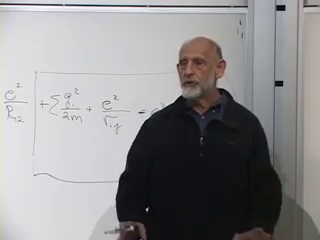
\includegraphics[width=0.72\textwidth]{lecture_01_figure_02.png}
\caption{Hamiltonian phân tử vẫn còn trên bảng khi bài toán trạng thái cơ bản điện tử được đưa ra. Dạng đánh máy trong phương trình~\eqref{eq:molecular-hamiltonian} ghi lại các hạng bị che khuất trong khung hình này.}
\lectureframe{00:16:19}
\end{figure}

\begin{classroomqa}
\audiencequestion{Có phải các xung lượng hạt nhân đơn giản là đang được đặt bằng không không?\lecturetimestamp{00:15:39}}
\lecturerresponse{Chỉ là tạm thời. Trong gần đúng bậc đầu, các hạt nhân được coi như bị ghim chặt vì chúng chuyển động chậm hơn electron rất nhiều. Xung lượng của chúng sẽ được khôi phục khi ta giải bài toán hạt nhân hiệu dụng, nên gần đúng này không vi phạm nguyên lý bất định.}
\end{classroomqa}

Năng lượng trạng thái cơ bản điện tử giờ đây đóng góp vào thế năng mà các hạt nhân cảm nhận:
\begin{equation}
V_{\mathrm{eff}}(R_1,R_2)
=\frac{e^2}{R_{12}}+E_{\mathrm{el}}(R_1,R_2).
\label{eq:molecular-effective-potential}
\end{equation}
Bất biến quay và tịnh tiến, đối với hai nguyên tử cô lập, thu gọn nó thành một hàm của khoảng cách giữa chúng \(R_{12}\). Ở khoảng cách rất ngắn, lực đẩy Coulomb hạt nhân chiếm ưu thế. Ở khoảng cách rất lớn thì hầu như không có tương tác. Giữa hai giới hạn đó, đám mây electron có thể tạo ra một vùng hút và một cực tiểu. Khi ấy, hàm sóng hạt nhân tập trung gần cực tiểu đó và mô tả một phân tử liên kết.

Hãy chú ý đến thứ tự các bước. Ta đã không đoán một lực hút thực nghiệm rồi bỏ các electron đi. Trước hết ta giải bài toán lượng tử của chúng trong nền hạt nhân cố định. Chỉ sau đó ta mới xóa các tọa độ tường minh của chúng và giữ lại trị riêng thu được. Vật lý khoảng cách ngắn vẫn còn trong hình dạng, độ sâu và độ cong của \(V_{\mathrm{eff}}\). Vị trí cực tiểu của nó đặt ra khoảng cách cân bằng, độ cong của nó chi phối các dao động nhỏ, và dạng tiệm cận của nó quyết định liệu có tồn tại trạng thái liên kết hay không. Một hàm hiệu dụng duy nhất mang toàn bộ thông tin điện tử đó vào bài toán chậm hơn.

Như vậy, một Hamiltonian nhiều electron phức tạp đã trở thành một Hamiltonian hạt nhân hai vật với một thế năng mới. Ta đã loại bỏ các bậc tự do nhanh, nhưng vẫn giữ lại trọn vẹn hiệu ứng năng lượng thấp của chúng. Thế năng đã được tái chuẩn hóa. Lập luận Born--Oppenheimer quen thuộc này thường không được giới thiệu dưới tên đó, nhưng nó chứa chính xác ý tưởng ta cần:
\begin{equation}
\begin{gathered}
\text{fast microscopic dynamics}\\
\Downarrow\\
\text{effective parameters for slow dynamics}
\end{gathered}
\end{equation}

\section{Đơn vị tự nhiên và thứ nguyên của một trường}

Trong lý thuyết trường lượng tử, các mode cần bị loại bỏ có thể được mô tả tương đương như các mode khoảng cách ngắn, bước sóng ngắn, tần số cao hoặc năng lượng cao. Trước khi vẽ giản đồ, ta hãy thống nhất cách theo dõi thứ nguyên.

Cơ học thông thường dùng các đơn vị độc lập cho độ dài, thời gian và khối lượng. Trong vật lý hạt, ta đặt
\begin{equation}
\hbar=c=1.
\end{equation}
Khi đó năng lượng và khối lượng là tương đương theo \(E=mc^2\), độ dài và thời gian là tương đương vì \(c=1\), và \(\hbar=1\) khiến xung lượng là nghịch đảo của độ dài. Chỉ còn lại một thứ nguyên:
\begin{equation}
[M]=[E]=[p]=L^{-1},
\qquad
[x]=[t]=L.
\label{eq:natural-units}
\end{equation}

Điều này không xóa bỏ thứ nguyên. Nó chọn các hệ số chuyển đổi sao cho một khoảng thời gian có thể được biểu diễn như một độ dài và một khối lượng như nghịch đảo của độ dài. Một khi đã chỉ định một đơn vị, mọi đơn vị khác đều suy ra theo. Vì thế, một ngưỡng cắt có thể được mô tả hoặc là một khoảng cách ngắn \(\delta\) hoặc là một năng lượng cao \(\Lambda=1/\delta\): đó là cùng một thang đo được diễn đạt bằng hai ngôn ngữ.

Xét một trường vô hướng thực \(\phi\), với mật độ Lagrangian được chuẩn hóa theo dạng sơ lược
\begin{equation}
\mathcal L=(\partial_\mu\phi)(\partial^\mu\phi)-V(\phi),
\qquad
S=\int d^4x\,\mathcal L.
\label{eq:scalar-action}
\end{equation}

\begin{figure}[htbp]
\centering
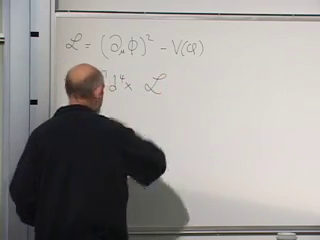
\includegraphics[width=0.78\textwidth]{lecture_01_figure_03.png}
\caption{Mật độ Lagrangian vô hướng cục bộ và tích phân không-thời gian của nó tạo thành tác dụng.}
\lectureframe{00:26:08}
\end{figure}

Mật độ Lagrangian là cục bộ: nó mô tả một điểm không-thời gian. Các phương trình trường cổ điển thu được bằng cách làm cho tác dụng dừng. Trong lý thuyết lượng tử, cũng chính tác dụng ấy xuất hiện trong pha của tích phân đường \(\exp(iS)\). Dù nhìn theo cách nào, thứ nguyên của \(S\) cũng là yếu tố quyết định. Khi khôi phục \(\hbar\), pha là \(\exp(iS/\hbar)\); sau khi đặt \(\hbar=1\), bản thân \(S\) phải là vô thứ nguyên.

\begin{classroomqa}
\audiencequestion{Tác dụng có đơn vị là \(\hbar\) không?\lecturetimestamp{00:26:13}}
\lecturerresponse{Có. Vì \(\hbar\) đã được đặt bằng một, nên tác dụng là vô thứ nguyên trong hệ đơn vị này. Phần tử đo bốn chiều có thứ nguyên \(L^4\), nên mật độ Lagrangian phải có thứ nguyên \(L^{-4}\).}
\end{classroomqa}

Bây giờ hạng động năng xác định thứ nguyên của trường:
\begin{align}
[S]&=1, & [\mathcal L]&=L^{-4},\\
[\partial_\mu]&=L^{-1}, &
[(\partial\phi)^2]&=L^{-2}[\phi]^2=L^{-4},\nonumber\\
&& [\phi]&=L^{-1}.
\label{eq:scalar-dimension}
\end{align}
Phép tính nhỏ này sẽ quyết định bậc tử ngoại của mọi giản đồ tiếp theo.

Khai triển thế năng thành
\begin{equation}
V(\phi)=\frac{m^2}{2}\phi^2+g\phi^3+\lambda\phi^4+\cdots.
\label{eq:scalar-potential}
\end{equation}
Mỗi hạng phải có thứ nguyên \(L^{-4}\). Vì \([\phi^n]=L^{-n}\),
\begin{equation}
[m^2]=L^{-2},
\qquad
[g]=L^{-1},
\qquad
[\lambda]=1.
\label{eq:coupling-dimensions}
\end{equation}
Hằng ghép bậc bốn là vô thứ nguyên. Những hằng ghép như vậy đặc biệt quan trọng trong tái chuẩn hóa vì sự phụ thuộc theo thang đo của chúng không thể đọc ra từ một lũy thừa đơn giản của độ dài.

\begin{classroomqa}
\audiencequestion{\(g\) có đơn vị của khối lượng không?\lecturetimestamp{00:29:52}}
\lecturerresponse{Có. Thừa số \(\phi^3\) có thứ nguyên \(L^{-3}\), còn mật độ thế năng phải có thứ nguyên \(L^{-4}\). Do đó \([g]=L^{-1}\), tức là khối lượng trong đơn vị tự nhiên.}
\end{classroomqa}

\section{Các đỉnh và hàm truyền ở khoảng cách ngắn}

Các quy tắc Feynman được xây dựng từ các đỉnh và các hàm truyền. Hạng \(g\phi^3\) cho một đỉnh ba đường mang một hệ số tỉ lệ với \(g\); \(\lambda\phi^4\) cho một đỉnh bốn đường mang một hệ số tỉ lệ với \(\lambda\). Hạng bậc hai cho một phép chèn hai điểm cục bộ. Có thể hình dung nó như một hạt đi vào, bị hấp thụ, rồi được phát ra trở lại, với hệ số tỉ lệ với \(m^2/2\). Các chuẩn hóa số, dấu, các thừa số của \(i\) và các hệ số đối xứng đều cố ý được lược bỏ vì bài giảng đang rút ra sự phụ thuộc theo thang đo chứ không tính một tiết diện tán xạ.

Các hình vẽ này có một cách hiểu theo thao tác. Một đỉnh ba điểm có thể hấp thụ hai lượng tử và phát ra một lượng tử, hoặc biểu diễn bất kỳ cách gán nào cho ba đường của nó liên hệ với đó qua phép crossing. Một đỉnh bốn điểm có thể mô tả hai hạt đi vào và hai hạt đi ra. Dấu chữ thập bậc hai vẫn là một đỉnh hai đường hoàn toàn hợp lệ dù thông thường nó được gộp vào hàm truyền tự do. Ta vẽ nó ra vì mọi quá trình hai điểm chưa được phân giải rồi sẽ sớm được nhận ra bằng cách so sánh với nó.

Một hàm truyền nối hai điểm không-thời gian. Đường của nó không phải là khẳng định rằng một hạt lượng tử đã đi theo một quỹ đạo cổ điển thẳng. Nó biểu diễn biên độ để tạo ra một kích thích trường tại \(x\) và loại bỏ hoặc dò được nó tại \(y\):
\begin{equation}
\Delta(x-y)=\langle0|\phi(y)\phi(x)|0\rangle.
\label{eq:position-propagator}
\end{equation}
Hãy đọc biểu thức từ bên phải. Tác dụng lên chân không bằng \(\phi(x)\) tạo ra một thành phần một hạt tại \(x\). Tác dụng \(\phi(y)\) lên bra loại bỏ thành phần tại \(y\). Phần tử ma trận chân không của chúng là biên độ chồng lấp giữa sự tạo ra ở điểm thứ nhất và sự dò được ở điểm thứ hai. Các ký hiệu \(x\) và \(y\) chỉ toàn bộ các bốn-vectơ, không chỉ đơn thuần là hai tọa độ Descartes.

Các trạng thái không mang thứ nguyên vật lý, còn mỗi trường đóng góp \(L^{-1}\). Vì vậy
\begin{equation}
[\Delta]=L^{-2}.
\end{equation}
Đối với một trường không khối lượng, không có thang độ dài nội tại nào, nên phân tích thứ nguyên buộc hành vi ở khoảng cách ngắn phải là
\begin{equation}
\Delta(x-y)\sim\frac{1}{(x-y)^2}.
\label{eq:massless-propagator}
\end{equation}
Mẫu số là bình phương độ tách bất biến Lorentz, kèm theo quy định thông thường cần dùng tại các điểm kỳ dị của nó.\editorialnote{Để đếm lũy thừa, thuận tiện là thực hiện phép quay Wick sang độ tách Euclid, khi đó độ lớn rõ ràng tỉ lệ với \(1/|x-y|^2\). Điều này không làm thay đổi các lũy thừa tử ngoại được dùng bên dưới.}

Khi \(y\) tiến tới \(x\), hàm truyền phân kỳ. Điểm kỳ dị này của sự truyền trên một độ tách tiêu biến là nguồn từ đó các phân kỳ tử ngoại trong những giản đồ phức tạp hơn được xây dựng nên.

\section{Khối lượng của trường vô hướng được tái chuẩn hóa như thế nào}

Đối với một trường vô hướng, tham số động lực học là \(m^2\), như hệ thức tán sắc tương đối tính đã gợi ý:
\begin{equation}
E=\sqrt{\mathbf p^2+m^2}.
\end{equation}
Gọi \(\delta\) là khoảng cách ngắn nhất mà mô tả hiệu dụng của ta phân giải được. Ta sẽ không phân biệt các quá trình có các đỉnh cách nhau ít hơn \(\delta\). Bất kỳ quá trình không phân giải được nào như vậy với một vô hướng đi vào và một vô hướng đi ra đều có cùng dạng hai điểm quan sát được như một phép chèn khối lượng và vì thế phải đóng góp vào khối lượng hiệu dụng.

Hãy xem máy gia tốc như một kính hiển vi. Nếu độ phân giải tốt nhất của nó là \(\delta\), thì một sự hấp thụ tại một điểm rồi tiếp theo là một sự phát ra ở một khoảng cách nhỏ hơn rất nhiều so với \(\delta\) sẽ không thể phân biệt được với một biến cố thực sự cục bộ. Ta cố ý làm mờ đỉnh trên thang đó. Tái chuẩn hóa là quy tắc chuyển tất cả những khả năng dưới độ phân giải như vậy vào hệ số của toán tử cục bộ tương ứng.

\subsection{Hiệu chỉnh bậc bốn thứ nhất}

Bắt đầu với một đỉnh \(\phi^4\) đơn lẻ. Hai chân là của hạt ngoài; hai chân kia nối lại thành một vòng ngắn được phát ra rồi hấp thụ lại gần như tại cùng một điểm. Làm mờ hàm truyền trùng điểm trên khoảng cách ngưỡng cắt cho
\begin{equation}
\Delta(0)\ \longrightarrow\ \Delta(\delta)\sim\frac{1}{\delta^2},
\end{equation}
và do đó
\begin{equation}
\delta m^2_{(1)}\sim\frac{\lambda}{\delta^2}.
\label{eq:one-loop-scalar-mass}
\end{equation}
Nếu \(m_0^2\) ký hiệu tham số đầu vào hay tham số trần, thì hệ số hai điểm ở độ phân giải thấp có dạng phác thảo
\begin{equation}
\frac{m_{\mathrm{eff}}^2}{2}
\sim
\frac{m_0^2}{2}
+c_1\frac{\lambda}{\delta^2},
\label{eq:first-renormalized-mass}
\end{equation}
trong đó \(c_1\) chứa các hệ số số học và phụ thuộc quy ước đã bị bỏ qua. Khối lượng đo được trong phòng thí nghiệm, trong những thí nghiệm không phân giải các khoảng cách nhỏ hơn \(\delta\), là đại lượng đã tái chuẩn hóa này, chứ không phải riêng \(m_0\).

Vì thế có hai cách không thể phân biệt được để biến cố hai điểm quan sát được xảy ra. Đỉnh bậc hai ban đầu có thể hấp thụ rồi phát lại hạt, hoặc tương tác bậc bốn có thể làm vậy trong khi thoáng chốc phát ra rồi hấp thụ lại một vô hướng ảo. Cơ học lượng tử cộng các biên độ. Một khi vòng nằm dưới thang phân giải, lịch sử riêng của nó biến mất khỏi mô tả hiệu dụng, nhưng đóng góp của nó vào hệ số đo được thì không.

\subsection{Hiệu chỉnh bậc bốn tiếp theo}

Bây giờ hãy nối hai đỉnh bậc bốn sao cho một hạt ngoài đi vào tại \(x\), một hạt đi ra từ \(x+\Delta\), và ba hàm truyền nội nối hai đỉnh. Có hai lũy thừa của \(\lambda\), còn các hàm truyền cho \(\Delta^{-6}\). Các biên độ lượng tử phải được cộng trên mọi vị trí không phân giải được mà tại đó hạt đi ra có thể xuất hiện, nên bốn-vectơ tương đối được lấy tích phân:
\begin{equation}
\delta m^2_{(2)}
\sim
\lambda^2
\int_{|\Delta|\gtrsim\delta}
d^4\Delta\,\frac{1}{|\Delta|^6}.
\label{eq:two-loop-power-count}
\end{equation}

\begin{classroomqa}
\audiencequestion{Dấu nhỏ ở đỉnh có nghĩa là ở đó chỉ có ba hạt thôi sao?\lecturetimestamp{00:46:35}}
\lecturerresponse{Không. Ta vẫn đang dùng tương tác bậc bốn. Bốn đường gặp nhau tại mỗi đỉnh; trong giản đồ hai điểm này một đường là ngoài và ba đường chạy giữa hai đỉnh. Đỉnh thứ hai lại có bốn đường đi vào nó.}
\end{classroomqa}

Phần tử đo đóng góp bốn lũy thừa của độ dài và ba hàm truyền đóng góp âm sáu. Vì ngưỡng cắt tử ngoại là thang duy nhất trong ước lượng này,
\begin{equation}
\int_{|\Delta|\gtrsim\delta}
\frac{d^4\Delta}{|\Delta|^6}
\sim\frac{1}{\delta^2},
\qquad
\delta m^2_{(2)}
\sim\frac{\lambda^2}{\delta^2}.
\label{eq:two-loop-scalar-mass}
\end{equation}
Ở đây \(\Delta^\mu\) là một biến tích phân bốn thành phần; ta tích phân theo thành phần thời gian và ba thành phần không gian của nó. Chữ thường \(\delta\) là ngưỡng cắt cố định. Ban đầu bài giảng dùng cùng một tên khi phát âm cho cả hai rồi về sau sửa lại ký hiệu.

Có thể thấy cùng kết quả bằng cách viết phần tử đo bốn chiều theo biến bán kính. Bỏ qua một hằng số góc,
\begin{equation}
\int_{\delta}\frac{d^4\Delta}{|\Delta|^6}
\sim
\int_{\delta}\frac{R^3\,dR}{R^6}
=\int_{\delta}\frac{dR}{R^3}
\sim\frac{1}{\delta^2}.
\end{equation}
Đó là lý do vì sao cận trên ở khoảng cách lớn không quan trọng đối với ước lượng tử ngoại: tích phân bị chi phối bởi đầu mút dưới của nó.

Các giản đồ bậc cao hơn lặp lại khuôn mẫu ấy. Một giản đồ với nhiều đỉnh bậc bốn hơn sẽ thêm một lũy thừa cao hơn của \(\lambda\), nhưng phân tích thứ nguyên vẫn cho phép một đóng góp khối lượng phân kỳ bậc hai:
\begin{equation}
\begin{aligned}
m_{\mathrm{eff}}^2
={}&m_0^2
+\frac{1}{\delta^2}
\left(c_1\lambda+c_2\lambda^2+c_3\lambda^3+\cdots\right)\\
&+\text{weaker terms}.
\end{aligned}
\label{eq:scalar-mass-series}
\end{equation}

\subsection{Tương tác bậc ba và một lôgarit}

Hai đỉnh bậc ba chứa hai hàm truyền giữa các điểm gần nhau. Đóng góp của chúng tỷ lệ như
\begin{equation}
\delta m_g^2
\sim
g^2\int_{|\Delta|\gtrsim\delta}
\frac{d^4\Delta}{|\Delta|^4}.
\label{eq:cubic-loop}
\end{equation}
Bây giờ phần tử đo và mẫu số mang các lũy thừa bằng nhau. Sự phụ thuộc còn lại là theo lôgarit chứ không phải theo lũy thừa:
\begin{equation}
\delta m_g^2
\sim
c_g g^2\log\!\left(\frac{1}{\mu\delta}\right).
\label{eq:cubic-log}
\end{equation}
Thang chuẩn \(\mu\) làm cho lôgarit trở thành không thứ nguyên. Đây là phiên bản có đủ thứ nguyên của biểu thức phác thảo trong bài giảng \(g^2\log\delta\). Một lôgarit biến thiên chậm hơn rất nhiều so với bất kỳ lũy thừa nghịch đảo nào, nên \(1/\delta^2\) trội hơn khi ngưỡng cắt trở nên nhỏ.

Một lần nữa, dạng theo bán kính làm cho sự khác biệt hiện ra rõ ràng:
\begin{equation}
\int_{\delta}^{R_{\mathrm{IR}}}
\frac{d^4\Delta}{|\Delta|^4}
\sim
\int_{\delta}^{R_{\mathrm{IR}}}\frac{R^3\,dR}{R^4}
=\log\!\left(\frac{R_{\mathrm{IR}}}{\delta}\right).
\end{equation}
Các lũy thừa bằng nhau ở phần tử đo và mẫu số sinh ra một lôgarit. Nhiều lũy thừa hơn ở mẫu số sinh ra một lũy thừa nghịch đảo của ngưỡng cắt. Bài giảng không yêu cầu ta tính các hệ số góc; nó dạy ta nhận ra đáp án tử ngoại ngay khi nhìn thấy.

\begin{classroomqa}
\audiencequestion{Lôgarit được lấy theo cơ số nào?\lecturetimestamp{00:57:42}}
\lecturerresponse{Hãy dùng lôgarit tự nhiên. Việc đổi cơ số chỉ nhân nó với một hằng số số học, và hằng số đó được hấp thụ vào hệ số mà các thừa số \(2\), \(\pi\) và các hệ số đối xứng của nó chưa được tính ở đây.}
\end{classroomqa}

\begin{classroomqa}
\audiencequestion{Làm sao có thể lấy lôgarit của một độ dài, và thứ nguyên của hiệu chỉnh khối lượng đến từ đâu?\lecturetimestamp{00:58:32}}
\lecturerresponse{Lôgarit luôn so sánh hai thang; nói cho đúng, đó là lôgarit của một tỉ số không thứ nguyên như \(1/(\mu\delta)\). Hằng ghép \(g\) có một lũy thừa khối lượng, nên \(g^2\) đã có đúng thứ nguyên bình phương khối lượng cần cho hiệu chỉnh.}
\end{classroomqa}

\begin{classroomqa}
\audiencequestion{Một giản đồ Feynman cho một biên độ. Bình phương độ lớn của nó có phải là một xác suất không?\lecturetimestamp{00:59:41}}
\lecturerresponse{Có, khi biên độ được đặt vào một phép tính chuyển tiếp vật lý với các thừa số trạng thái và không gian pha cần thiết. Ở đây vai trò trực tiếp hơn của nó lại khác: một biên độ hai điểm không phân giải được có cùng dạng cục bộ như hạng khối lượng và vì thế làm dịch chuyển tham số khối lượng hiệu dụng.}
\end{classroomqa}

\section{Mọi tham số đều trở thành hiệu dụng}

Họ vô hạn các giản đồ khối lượng không biến mất chỉ vì \(\lambda\) nhỏ. Lý thuyết nhiễu loạn sắp xếp chúng theo các lũy thừa của hằng ghép, nên các hạng kế tiếp có thể nhỏ dần, nhưng vẫn có vô hạn hạng. Việc loại bỏ khoảng cách ngắn ấy cũng tái chuẩn hóa chính các tương tác.

\begin{classroomqa}
\audiencequestion{Ngay cả đối với tái chuẩn hóa khối lượng, chẳng phải cũng có vô hạn giản đồ sao?\lecturetimestamp{01:00:35}}
\lecturerresponse{Đúng là có. Nếu \(\lambda\) đủ nhỏ thì chuỗi nhiễu loạn có thể hữu ích vì các lũy thừa cao hơn bị dập tắt dần. Tuy nhiên, tham số đã tái chuẩn hóa được xác định bởi toàn bộ chuỗi, chứ không chỉ bởi hình vẽ đầu tiên thôi.}
\end{classroomqa}

Về mặt thao tác, một tương tác cục bộ \(\lambda\phi^4\) là một biên độ hai hạt vào, hai hạt ra. Nếu một quá trình bốn điểm phức tạp hơn xảy ra hoàn toàn bên trong một vùng không phân giải được, thì ở độ phân giải thấp nó không thể phân biệt được với đỉnh cục bộ ban đầu. Vì thế các giản đồ như vậy được gộp vào một \(\lambda\) hiệu dụng. Sự phụ thuộc theo thang chủ đạo của chúng trong lý thuyết \(\phi^4\) bốn chiều thường là theo lôgarit. Bài giảng không tính hàm beta đó; nó dùng ví dụ này để phát biểu mệnh đề tổng quát:
\begin{equation}
\begin{gathered}
\text{parameters measured at low energy}\\
\ne\\
\text{parameters entered at the microscopic cutoff}
\end{gathered}
\end{equation}

Ví dụ bốn điểm quan trọng vì nó loại bỏ một khả năng hiểu sai. Tái chuẩn hóa không phải là một phép sửa chữa đặc biệt chỉ áp dụng cho một phân kỳ khối lượng. Mọi toán tử được phép trong Lagrangian đều có thể được tái tạo bởi các giản đồ không phân giải được có cùng các chân ngoài và các đối xứng. Một quá trình hai điểm tái chuẩn hóa một hệ số bậc hai, một quá trình bốn điểm tái chuẩn hóa một hệ số bậc bốn, và các quá trình từ chân không đến chân không sẽ tái chuẩn hóa hạng hằng. Lagrangian năng lượng thấp là sổ cái cô đọng trong đó mọi quá trình khoảng cách ngắn ấy được ghi lại.

\begin{classroomqa}
\audiencequestion{Vì \(\Delta\) có đơn vị độ dài, phải chăng lấy lôgarit của nó là lạ về mặt thứ nguyên? Và trên bảng có đổi lẫn delta viết hoa với viết thường không?\lecturetimestamp{01:01:34}}
\lecturerresponse{Lôgarit thực ra có nghĩa là một tỉ số với một thang khác và vì thế là không thứ nguyên. Đúng, ký hiệu đã bị đổi lẫn trong chốc lát: \(\Delta^\mu\) là biến tích phân, còn \(\delta\) là ngưỡng cắt khoảng cách ở cận dưới còn lại trong đáp án.}
\end{classroomqa}

Đây là đối ứng trong lý thuyết trường của phân tử. Ta đã giải đối với các electron nhanh không nhìn thấy và đưa kết quả của chúng vào một thế. Ở đây ta cộng các quá trình khoảng cách ngắn không nhìn thấy và đưa kết quả của chúng vào các khối lượng, các hằng ghép và mọi hệ số cục bộ được phép khác. Mọi thứ đều bị dịch chuyển.

\begin{classroomqa}
\audiencequestion{Thầy có thể nhắc lại liệu đại lượng đo được có bao gồm các thang nhỏ hơn mức thí nghiệm có thể thấy hay không không?\lecturetimestamp{01:05:13}}
\lecturerresponse{Có. Những thăng giáng riêng lẻ của chúng không được phân giải, nhưng hiệu ứng tổng cộng của chúng thì có mặt. Mọi giản đồ liên quan đến các thang ngắn hơn đều được gộp vào một hệ số hiệu dụng duy nhất mà một thí nghiệm năng lượng thấp gọi, chẳng hạn, là bình phương khối lượng vật lý.}
\end{classroomqa}

\begin{classroomqa}
\audiencequestion{Vậy số hạng đầu vào \(m_0^2\) có phải triệt tiêu các đóng góp khác không?\lecturetimestamp{01:06:00}}
\lecturerresponse{Nếu khối lượng vô hướng đo được nhỏ hơn rất nhiều so với các đóng góp tử ngoại riêng lẻ, thì đúng vậy. Sự triệt tiêu cần thiết ấy chính là bài toán tinh chỉnh mà bây giờ ta chuyển sang.}
\end{classroomqa}

\section{Bài toán phân cấp Higgs}

Hãy hình dung ngưỡng cắt là độ dài Planck, để lý thuyết trường hiệu dụng được yêu cầu tóm lược các thăng giáng từ những thang phòng thí nghiệm xuống tới thang mà hấp dẫn lượng tử buộc phải can thiệp.
Trong các đơn vị của vật lý hạt,
\begin{equation}
\delta\sim M_{\mathrm{Pl}}^{-1}\sim10^{-19}\,\mathrm{GeV}^{-1},
\qquad
\frac{1}{\delta^2}\sim10^{38}\,\mathrm{GeV}^2.
\label{eq:planck-cutoff}
\end{equation}
Việc dùng chính xác thang Planck rút gọn hay không rút gọn không quan trọng đối với phép so sánh khổng lồ này.

Phân cấp về khoảng cách cũng nổi bật không kém. Độ dài Planck nhỏ hơn bán kính proton khoảng 19 bậc độ lớn và nhỏ hơn các khoảng cách được các máy gia tốc đang được bàn đến thăm dò trực tiếp khoảng 16 hoặc 17 bậc. Việc bình phương độ tách ấy chính là điều biến một phân cấp độ dài lớn thành sự triệt tiêu cỡ 34 chữ số trong một tham số bình phương khối lượng vô hướng.

Đối với trường Higgs, một trường vô hướng, thang yếu mong muốn có cỡ vài trăm GeV, chứ không phải \(10^{19}\) GeV. Thế nhưng các hạng trong Phương trình~\eqref{eq:scalar-mass-series} một cách tự nhiên có thể có cỡ thang Planck. Dấu của chúng chưa được theo dõi: một số có thể dương và một số có thể âm, và bình phương khối lượng trần cũng có thể mang một trong hai dấu. Nhưng để còn lại một phần dư ở thang điện yếu, những phần khổng lồ ấy phải triệt tiêu nhau tới khoảng 34 chữ số thập phân. Ban đầu Susskind nói 17 chữ số, rồi tự sửa lại vì phép so sánh là giữa các bình phương khối lượng. Chính tỉ số đã được bình phương mới đo phiên bản tinh chỉnh này.

\begin{classroomqa}
\audiencequestion{\(\lambda\) nhỏ hơn hay lớn hơn 1?\lecturetimestamp{01:09:50}}
\lecturerresponse{Người ta giả định nó nhỏ hơn 1 ở mức vừa phải. Lý thuyết nhiễu loạn sẽ trở nên khó xử lý nếu các lũy thừa kế tiếp tăng lên, và một lý thuyết vô hướng thuần túy cũng không thể được ngoại suy một cách nhất quán với một hằng số liên kết tứ bậc lớn tùy ý. Nhưng \(\lambda\) hoàn toàn không nhỏ đến mức như \(10^{-38}\); bài giảng lấy một con số cỡ phần trăm để định hướng.}
\end{classroomqa}

\begin{classroomqa}
\audiencequestion{Ngay cả khi \(\lambda<1\), chẳng phải vẫn còn nhiều hạng giữ vai trò quan trọng vì mỗi hạng đều mang hệ số cắt lớn sao?\lecturetimestamp{01:10:43}}
\lecturerresponse{Đúng vậy. Các lũy thừa cao hơn rốt cuộc sẽ làm suy giảm chuỗi, nhưng trước khi điều đó thắng thế thì vẫn có thể có một tập hợp lớn các hạng đóng góp. Tất cả chúng, cùng với hạng trần, đều sẽ phải cùng nhau triệt tiêu tinh vi để còn lại đáp án vật lý nhỏ phi thường ấy.}
\end{classroomqa}

Nhắc lại vì sao tham số khối lượng Higgs được biết là ở thang yếu. Theo quy ước của bài giảng, viết thế phá vỡ đối xứng dưới dạng
\begin{equation}
V(\phi)=-\frac{\mu^2}{2}\phi^2+\frac{\lambda}{4}\phi^4.
\label{eq:higgs-potential}
\end{equation}
Hệ số bậc hai âm làm cho gốc tọa độ mất ổn định, còn hạng tứ bậc dương làm ổn định thế. Lấy đạo hàm,
\begin{equation}
\frac{dV}{d\phi}=-\mu^2\phi+\lambda\phi^3
=\phi(-\mu^2+\lambda\phi^2),
\end{equation}
cho ta cực tiểu khác không
\begin{equation}
\phi_{\min}^2=f^2=\frac{\mu^2}{\lambda}.
\label{eq:higgs-minimum}
\end{equation}
Trên bảng viết hạng tứ bậc một cách sơ lược là \(\lambda\phi^4\) nhưng lại viện dẫn phương trình ~\eqref{eq:higgs-minimum}; chèn hệ số quy ước \(1/4\) sẽ làm cho hai dòng ấy nhất quán với nhau mà không thay đổi lập luận.

Dấu của \(-\mu^2\) là quan trọng, nhưng không cứu được tính tự nhiên. Chính độ cong âm tại gốc tọa độ là cái thúc đẩy sự phá vỡ đối xứng tự phát. Tái chuẩn hóa làm dịch chuyển độ cong ấy bởi những phần dương và âm rất lớn. Chân không bị phá vỡ mà ta quan sát được đòi hỏi tổng của chúng không chỉ nhỏ, mà còn phải có đúng giá trị âm nhỏ đặc biệt đặt cực tiểu ở thang yếu.

Khối lượng của các boson \(W\) và \(Z\) xác định \(f\) vào cỡ \(200\,\mathrm{GeV}\) trong cách chuẩn hóa gần đúng được dùng trong bài giảng. Nếu \(\lambda\) không quá lớn cũng không nhỏ đến mức khó tin, thì \(\mu\) phải cùng bậc đại thể như vậy. Vì thế, hệ số quan sát được ở thang yếu là phần dư của những đóng góp mà mỗi cái riêng lẻ có thể lớn hơn nhiều chục bậc độ lớn.

Điều này được gọi là bài toán tinh chỉnh Higgs, bài toán phân cấp, hoặc bài toán phân cấp chuẩn. Phân cấp ở đây là tỉ số khổng lồ giữa thang yếu thông thường và một thang thống nhất hoặc Planck khả dĩ. Một số nhỏ tự nó chưa chắc đã là nghịch lý. Điều gây bất an ở đây là một số nhỏ được ghép từ những phần lớn, có vẻ không liên hệ với nhau, nhưng lại phải triệt tiêu nhau với độ chính xác cực cao. Bài toán này đã được nhận ra vào cuối thập niên 1970 và đầu thập niên 1980, và việc tìm một cơ chế đằng sau sự triệt tiêu ấy đã thúc đẩy siêu đối xứng cùng một số ý tưởng cạnh tranh khác.

Chuỗi nhiễu loạn vô hạn làm cho câu đố sắc nét hơn chứ không loại bỏ nó. Một \(\lambda\) cỡ phần trăm khiến các lũy thừa đủ cao trở nên nhỏ, nhưng có thể xuất hiện nhiều hạng trước khi sự suy giảm ấy thắng thế. Không đủ nếu một vòng tình cờ triệt tiêu khối lượng trần. Thang yếu hiệu dụng phải vẫn ổn định sau khi đã tính cả phần còn lại của các quá trình khoảng cách ngắn. Một quan hệ có tính cấu trúc giữa các hạng mới là lời giải thích; một sự triệt tiêu từng chữ số giữa những phần không liên hệ chỉ là tinh chỉnh.

\section{Vì sao khối lượng fermion ứng xử tốt hơn}

Các hạt khác của Mô hình Chuẩn không đòi hỏi những sự tinh chỉnh độc lập cùng loại. Với một fermion Dirac, hạng khối lượng là
\begin{equation}
\mathcal L_m=-m\bar\psi\psi
=-m\left(\bar\psi_L\psi_R+\bar\psi_R\psi_L\right).
\label{eq:fermion-mass}
\end{equation}
Nó chứa khối lượng, không phải bình phương của khối lượng, và nó nối chirality trái với chirality phải. Vì thế, một phép chèn khối lượng cục bộ biến \(L\) thành \(R\), hoặc \(R\) thành \(L\).

\begin{figure}[htbp]
\centering
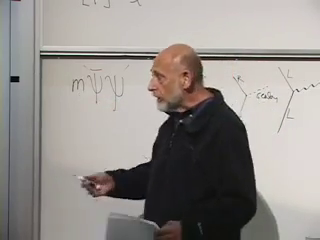
\includegraphics[width=0.76\textwidth]{lecture_01_figure_04.png}
\caption{Hạng khối lượng fermion và các phác họa đường làm đổi chirality trên bảng. Các hình được dựng lại bằng đại số ở dưới vì một phần nét phấn bị che khuất.}
\lectureframe{01:23:36}
\end{figure}

Trong phần trình bày miệng, giảng viên thường nói đến tính thuận tay hoặc helicity. Sự bảo vệ chính xác được phát biểu sáng sủa nhất theo chirality. Đối với một hạt siêu tương đối tính, hình dung theo helicity cung cấp trực giác mà bài giảng nhắm tới, nhưng chirality mới là đại lượng do các trường tay trái và tay phải trong phương trình~\eqref{eq:fermion-mass} mang.

Tương tác chuẩn bảo toàn chirality:
\begin{equation}
L\xrightarrow{\ \gamma\ }L,
\qquad
R\xrightarrow{\ \gamma\ }R.
\label{eq:gauge-preserves-chirality}
\end{equation}
Một tương tác Yukawa với một trường vô hướng nối hai chirality đối nhau:
\begin{equation}
L\xleftrightarrow{\ \phi\ }R.
\label{eq:scalar-flips-chirality}
\end{equation}
Trước hết, giả sử \(m_0=0\). Việc phát xạ rồi tái hấp thụ bất kỳ số photon nào cũng không thể sinh ra khối lượng, vì mọi đỉnh chuẩn đều bảo toàn chirality. Một chuỗi bắt đầu với chirality trái sẽ vẫn là chirality trái. Vì vậy, điện động lực học lượng tử thuần túy cho phép một electron không khối lượng một cách nhất quán: tự năng điện từ của nó không thể tạo ra một khối lượng cộng thêm từ số 0.

Trong hình ảnh đường, hãy bắt đầu với một electron có chirality trái. Ở đỉnh photon thứ nhất nó vẫn có chirality trái; sau khi truyền đi và tái hấp thụ photon nó vẫn có chirality trái. Lặp lại cấu trúc ấy chỉ chèn thêm các đỉnh bảo toàn chirality. Hàm hai điểm ngoài có thể được tái chuẩn hóa, nhưng nó không thể nhận được cấu trúc trái-phải vốn định nghĩa một khối lượng.

Phát xạ vô hướng có làm được điều đó không? Một đỉnh vô hướng biến \(L\) thành \(R\), nhưng một vô hướng đã phát ra thì phải được tái hấp thụ. Vì thế, một đồ thị tự năng hai điểm chứa một số chẵn các đỉnh vô hướng. Lần lật thứ hai đảo ngược lần thứ nhất, nên toàn bộ đồ thị lại bảo toàn chirality ngoài. Dù đồ thị bên trong có trở nên phức tạp đến đâu, phát xạ và tái hấp thụ vẫn ghép cặp các đỉnh và ngăn không cho xuất hiện một hạng cộng thêm từ \(L\) sang \(R\) khi khối lượng ban đầu bằng 0.

Đây là một lập luận chẵn-lẻ về số lần lật. Một đỉnh vô hướng lật chirality một lần; việc khép kín mỗi đường vô hướng nội đòi hỏi một đầu mút thứ hai và vì thế một lần lật thứ hai. Bốn đỉnh vô hướng lật bốn lần, v.v. Một số chẵn đưa fermion trở về chirality ban đầu của nó. Kết luận này không bị giới hạn ở vòng đơn giản nhất được vẽ trên bảng.

Một hiệu chỉnh khối lượng khác không chỉ trở nên khả dĩ sau khi sơ đồ đã chứa sẵn một phép chèn khối lượng. Chẳng hạn, sự phát xạ và tái hấp thụ photon có thể bao quanh một phép chèn \(m_0\bar\psi\psi\). Các đỉnh chuẩn đóng góp hai lũy thừa của điện tích điện, nhưng lần lật chirality duy nhất đóng góp khối lượng ban đầu:
\begin{equation}
\begin{aligned}
m_e
&=m_0+c_1e^2m_0+c_2e^4m_0+\cdots\\
&=m_0\left(1+c_1e^2+c_2e^4+\cdots\right).
\end{aligned}
\label{eq:multiplicative-fermion-mass}
\end{equation}
Nếu \(m_0=0\), kết quả vẫn bằng không. Nếu \(m_0\) nhỏ, thì mọi hiệu chỉnh đều tỉ lệ với số nhỏ ấy. Ta vẫn có thể hỏi vì sao electron lại nhẹ so với một thang cơ bản, nhưng ta không còn phải lấy những số khổng lồ không liên hệ mà trừ vào nhau để thu được nó nữa. Theo nghĩa này, một khối lượng fermion nhỏ là tự nhiên theo nghĩa kỹ thuật.

Phép chèn khối lượng làm cho chuỗi được phép trở nên tường minh. Bắt đầu với \(L\). Phát xạ photon bảo toàn \(L\); phép chèn \(m_0\) biến \(L\) thành \(R\); tái hấp thụ photon bảo toàn \(R\). Khi đó, sơ đồ có chirality ngoài của một hạng khối lượng, nhưng giá trị của nó tất yếu chứa thừa số \(m_0\). Đây là sự tương phản then chốt với phương trình ~\eqref{eq:one-loop-scalar-mass}, ở đó hiệu chỉnh vô hướng vẫn khác không ngay cả khi khối lượng vô hướng ban đầu được đặt bằng không.

Các boson chuẩn có một sự bảo vệ tương tự: đối xứng chuẩn cấm một hạng khối lượng độc lập, nên một boson chuẩn ban đầu không khối lượng sẽ vẫn không khối lượng ở mọi bậc nhiễu loạn. Trong Mô hình Chuẩn, khối lượng của các fermion và các boson chuẩn yếu phát sinh do giá trị kỳ vọng Higgs. Nếu kiểm soát được thang Higgs, thì các khối lượng nhẹ còn lại không cần những lần lặp riêng rẽ của cùng một sự tinh chỉnh thảm khốc ấy.

Điều này xác định câu hỏi mà siêu đối xứng được kỳ vọng sẽ giải quyết: liệu một lý thuyết có thể ngăn không cho vô hướng Higgs nhận một hiệu chỉnh khối lượng cộng thêm khổng lồ hay không? Câu trả lời là có trong những thiết lập siêu đối xứng thích hợp, vì các đóng góp boson và fermion có liên hệ với nhau chứ không độc lập. Cơ chế chi tiết bắt đầu ở bài giảng tiếp theo.

\section{Sự tinh chỉnh khác: năng lượng chân không}

Vẫn còn một bài toán tái chuẩn hóa còn nghiêm trọng hơn, nhưng nó chỉ trở nên quan sát được khi có hấp dẫn. Trong vật lý phi hấp dẫn, việc cộng một hằng số vào mọi năng lượng không làm thay đổi thí nghiệm nào. Chẳng hạn, khối lượng electron không phải là một năng lượng tuyệt đối; nó là năng lượng tăng thêm cần để thêm một electron vào chân không:
\begin{equation}
m_e=E(\text{vacuum}+\text{one electron})-E(\text{vacuum})
\end{equation}
trong hệ nghỉ của electron. Nếu chân không và mọi trạng thái kích thích cùng dịch chuyển, thì các hiệu của chúng vẫn không đổi.

Tuy vậy, các sơ đồ chân không-sang-chân không quả thật làm dịch chuyển năng lượng chân không. Trong lý thuyết \(\lambda\phi^4\), hãy nối bốn chân của một đỉnh tứ bậc thành hai vòng ngắn. Mỗi hàm truyền tại điểm trùng nhau cho \(1/\delta^2\), nên
\begin{equation}
\delta\rho_{\mathrm{vac}}
\sim
c_{\mathrm{vac}}\frac{\lambda}{\delta^4}.
\label{eq:vacuum-energy-divergence}
\end{equation}
Các sơ đồ chân không phức tạp hơn mang những hệ số liên kết và hệ số số học khác nhau, nhưng phân tích thứ nguyên thường vẫn để lại cùng một độ nhạy điểm cắt bậc bốn đối với một mật độ năng lượng.

Chính việc không có các đường ngoài là dấu hiệu nhận ra hiệu chỉnh này. Các đồ thị hai điểm so sánh một trạng thái một hạt với chân không và làm thay đổi khối lượng; các đồ thị bốn điểm làm thay đổi tán xạ; một đồ thị không có hạt đi vào hay đi ra làm thay đổi chính biên độ chân không-sang-chân không. Một đỉnh tứ bậc cho \(\lambda\), và hai vòng ngắn của nó cho \(\delta^{-2}\) mỗi vòng. Khi đó, phân tích thứ nguyên đòi hỏi thang mật độ năng lượng \(\delta^{-4}\).

Không có hấp dẫn, ta có thể chọn mốc 0 cộng tính của năng lượng và hỏi ai quan tâm. Thuyết tương đối rộng tước bỏ tự do ấy: tensor năng lượng-động lượng là nguồn của độ cong không-thời gian, nên một năng lượng chân không đồng đều làm cho không gian trống hấp dẫn. Nó xuất hiện như một hằng số vũ trụ và được liên hệ về mặt quan sát với năng lượng tối. Khi đó, một năng lượng chân không đo được rất nhỏ phải còn lại sau những đóng góp có dạng \(\delta^{-4}\).

Đó là lý do vì sao câu hỏi thay đổi khi đưa hấp dẫn vào. Trong cơ học lượng tử thông thường, dịch mọi mức lên cùng một hằng số không làm động đến bất kỳ tần số chuyển mức nào. Trong hấp dẫn, hằng số ấy không trơ: tensor năng lượng-động lượng của chân không tỉ lệ với metric và làm cong không-thời gian. Điều từng là một mốc 0 năng lượng tùy ý nay trở thành một nguồn trong phương trình Einstein.

Vì vậy có ít nhất hai câu đố về tính tự nhiên ở mức cực đoan. Bài giảng nêu xấp xỉ 123 chữ số thập phân cho mức tinh chỉnh của năng lượng chân không và khoảng 30--35 cho mức tinh chỉnh của khối lượng Higgs. Số lượng chính xác phụ thuộc vào thang tử ngoại và các quy ước, nhưng sự tương phản thì không có gì phải nghi ngờ. Siêu đối xứng là một lời đáp tiềm năng cho bài toán Higgs được bàn ở đây; một khi siêu đối xứng bị phá vỡ, tự thân nó không giải thích được hằng số vũ trụ học quan sát được.\editorialnote{Đây cũng là lý do vì sao một sự triệt tiêu boson--fermion siêu đối xứng chính xác không phải là một lời giải hiện tượng học cho năng lượng chân không quan sát được: siêu đối xứng phải bị phá vỡ trong thế giới của chúng ta.}

\section{Các câu hỏi cuối buổi học}

\begin{classroomqa}
\audiencequestion{Hiệu chỉnh Higgs phụ thuộc vào điểm cắt \(\delta\), nhưng điểm cắt ấy có vẻ tùy ý. Nó có thể là độ dài Planck, gấp 10 lần độ dài Planck, hay một thứ khác không? Điều đó có làm cho sự tinh chỉnh trở nên tùy ý không?\lecturetimestamp{01:33:50}}
\lecturerresponse{Đóng góp số học phụ thuộc vào thang ngắn nhất mà lý thuyết hiệu dụng còn được tin cậy. Sự phụ thuộc ấy là cách hạch toán vật lý, không phải một lối thoát. Các mode đến bất kỳ thang nào mà Mô hình Chuẩn vẫn còn có nghĩa đều là những mode mà hiệu ứng của chúng phải được tính vào. Chọn \(\delta\) tại khoảng cách nơi người ta kỳ vọng có vật lý mới---có thể là thang Planck, có thể là một thang thống nhất gần \(10^{16}\,\mathrm{GeV}\). Đóng góp tích lũy xuống đến thang ấy đã là một cận dưới cho vấn đề rồi. Mở rộng cùng lý thuyết ấy xuống những khoảng cách còn ngắn hơn chỉ làm cho độ nhạy bậc hai lớn hơn. Ta có nghĩa vụ phải giải thích điều gì triệt tiêu đóng góp từ mọi thang giữa phòng thí nghiệm và biên tử ngoại ấy.}
\end{classroomqa}

\begin{classroomqa}
\audiencequestion{Điều gì định nghĩa một hạt vô hướng, và ví dụ là gì?\lecturetimestamp{01:37:26}}
\lecturerresponse{Ví dụ được nhắm đến là Higgs. Một trường vô hướng không biến đổi thành các thành phần khác nhau dưới một phép quay không gian; tương đương, các lượng tử hạt của nó có spin 0. Photon được mô tả bởi một trường vectơ, còn trường hấp dẫn bởi một tenxơ. Vào thời điểm của bài giảng 2010 này, vẫn chưa phát hiện được hạt sơ cấp spin 0 nào.\editorialnote{Boson Higgs được phát hiện tại CERN vào 2012 và các tính chất đo được của nó phù hợp với spin 0.}}
\end{classroomqa}

\begin{classroomqa}
\audiencequestion{Hạt \(Z\) cũng là một boson chuẩn phải không?\lecturetimestamp{01:38:31}}
\lecturerresponse{Có. \(Z\), \(W^+\) và \(W^-\) là các boson chuẩn spin 1; photon cũng vậy. Các phương trình trường và các tương tác của chúng là những khái quát hóa không Abel hoặc điện yếu của mô tả chuẩn kiểu Maxwell.}
\end{classroomqa}

\begin{classroomqa}
\audiencequestion{Tại sao đóng góp của trạng thái cơ bản boson lại không triệt tiêu đóng góp của trạng thái cơ bản fermion trong năng lượng chân không?\lecturetimestamp{01:39:10}}
\lecturerresponse{Các vòng fermion và các vòng boson tương ứng quả thật có thể xuất hiện với dấu đối nhau. Tuy nhiên, sự triệt tiêu không tự động xảy ra: khối lượng, số bội và các hằng số ghép của hạt phải khớp nhau. Chỉ một sai lệch nhỏ cũng để lại một phần dư lớn nhạy với ngưỡng cắt, và các họ giản đồ vô hạn phải khớp nhau theo từng bậc. Siêu đối xứng chính xác áp đặt chính những quan hệ boson--fermion như vậy. Thành phần hạt không siêu đối xứng nói chung thì không như vậy, và siêu đối xứng bị phá vỡ để lại một bài toán năng lượng chân không còn dư.}
\end{classroomqa}

\section{Toàn cảnh}

Lộ trình của bài giảng được sắp đặt có chủ ý. Trước hết, một phép tính phân tử cho thấy rằng việc loại bỏ các biến nhanh không phải là bỏ qua chúng, cũng không phải là phép màu: năng lượng trạng thái cơ bản của chúng trở thành một thế năng đối với các biến chậm. Lý thuyết trường lượng tử lặp lại thao tác đó trên các thang bước sóng. Phân tích thứ nguyên sau đó cho thấy những tham số hiệu dụng nào nhạy với ngưỡng cắt. Khối lượng của các hạt vô hướng nhận các số hạng cộng thêm tỉ lệ với \(\delta^{-2}\); vì vậy, một thang Higgs nhỏ có vẻ mong manh một cách không tự nhiên. Khối lượng fermion được tái chuẩn hóa theo kiểu nhân vì tính tay bảo vệ giới hạn khối lượng bằng không, và đối xứng chuẩn cũng bảo vệ tương tự các boson chuẩn không khối lượng. Năng lượng chân không còn nhạy hơn nữa, có tỉ lệ như \(\delta^{-4}\), và hấp dẫn khiến giá trị tuyệt đối của nó có thể quan sát được.

Siêu đối xứng được đưa vào chính tại điểm này, không phải như một thứ toán học mới mang tính trang trí mà như một nỗ lực làm cho sector vô hướng ứng xử giống các sector được bảo vệ hơn. Nhiệm vụ tiếp theo là hiểu xem đối xứng nào có thể liên hệ boson với fermion đủ chặt chẽ để sắp đặt các sự triệt tiêu đó.

\chapter{Dấu fermion và các triệt tiêu siêu đối xứng}

\lectureoverview{Siêu đối xứng liên hệ boson với fermion, nhưng lý do muốn có một quan hệ như vậy dễ thấy hơn trước khi viết ra đại số của nó. Chúng ta bắt đầu từ tôpô của các phép quay, làm cho dấu của hàm sóng fermion trở nên quan sát được thông qua giao thoa, suy ra dấu âm của một vòng fermion kín từ phản đối xứng khi hoán đổi, rồi dùng các dấu vòng trái ngược nhau của boson và fermion để gợi ý sự triệt tiêu của năng lượng chân không và của tự năng vô hướng. Nửa sau đặt câu hỏi siêu đối xứng có thể bị phá vỡ nặng đến mức nào, người ta có thể phát hiện các siêu đối hạt bằng cách nào, và vì sao siêu đối xứng chính xác sẽ xóa bỏ cấu trúc lớp vỏ nguyên tử thông thường.}

\section{Trước siêu đối xứng: một điểm kỳ lạ của các phép quay}

Siêu đối xứng là một đối xứng giữa fermion và boson. Tuy nhiên, trước khi thử xây dựng nó, đáng để nhớ lại hai loại hạt này biến đổi khác nhau ra sao dưới các phép quay. Bản thân câu hỏi ấy bắt đầu từ một sự kiện tôpô dễ minh họa nhưng lại khó quên một cách đáng ngạc nhiên một khi đã thấy nó.

Đưa một bàn tay lên, lòng bàn tay ngửa, rồi xoay cổ tay một góc \(2\pi\). Bàn tay trở lại đúng hướng ban đầu, nhưng rõ ràng cánh tay chưa trở lại một cấu hình tương đương: nó bị xoắn. Tiếp tục thêm một \(2\pi\) nữa, đồng thời dịch chuyển cánh tay khi cần, thì có thể gỡ xoắn. Vì thế một phép quay \(2\pi\) không thể được biến dạng liên tục thành không quay khi môi trường xung quanh được giữ cố định, còn một phép quay \(4\pi\) thì có thể. Minh họa bằng bàn tay này là một chứng minh bằng vung tay theo đúng nghĩa đen nhất.

Cùng điểm đó có thể được nêu ra mà không cần dựa vào giải phẫu học. Đặt một quả bóng trong một chiếc hộp cố định và nối quả bóng với các thành hộp bằng một số bất kỳ các sợi dây mềm, co giãn được nhưng không thể đứt. Quay quả bóng một vòng \(2\pi\). Các sợi dây bị rối, và không chuyển động nào chỉ của riêng chúng có thể khôi phục cấu hình ban đầu. Quay quả bóng đến tổng góc \(4\pi\), và có thể luồn các sợi dây đi vòng quanh nó cho đến khi chỗ rối biến mất. Các bức tường tượng trưng cho vô cùng không gian: phép so sánh chỉ có nghĩa vì biên không bị quay cùng với quả bóng.

\begin{classroomqa}
\audiencequestion{Có thể gỡ chỗ rối đó bằng cách quay cái hộp không? \lecturetimestamp{00:02:53}}
\lecturerresponse{Như thế là thay đổi bài toán. Cái hộp biểu trưng cho vô cùng không gian và được giữ cố định. Ta đang so sánh phép quay của vật so với môi trường xung quanh nó, chứ không phải một phép quay chung của cả vật lẫn môi trường.}
\end{classroomqa}

\begin{classroomqa}
\audiencequestion{Vì sao không đơn giản quay quả bóng thêm một \(2\pi\) nữa? \lecturetimestamp{00:03:20}}
\lecturerresponse{Chính đó là điều phân biệt hai trường hợp. Nếu không quay quả bóng thêm nữa, chỗ rối để lại sau một vòng \(2\pi\) không thể gỡ được. Sau vòng thứ hai, cho tổng cộng \(4\pi\), thì có thể.}
\end{classroomqa}

Trong ngôn ngữ nhóm hiện đại, nhóm quay có hai lớp tôpô của các đường khép kín:
\begin{equation}
\pi_1\!\left(SO(3)\right)\cong \mathbb Z_2.
\end{equation}
Đi một vòng là không tầm thường, nhưng đi hai vòng thì cho lớp tầm thường.
Tương đương, \(SU(2)\) là phủ đôi của \(SO(3)\). Đây là phần tiền sử hình học của dấu fermion.

\editorialnote{Ngôn ngữ của \(SO(3)\), \(SU(2)\) và nhóm cơ bản làm cho cấu trúc tôpô trở nên tường minh. Minh họa bằng cánh tay và minh họa bằng dây xác lập cùng một tính hai trị về mặt hình học.}

\section{Phép quay \texorpdfstring{\(2\pi\)}{2 pi} tác động gì lên một trạng thái lượng tử}

Bây giờ hãy cố định vị trí của một hạt và chỉ giữ lại trạng thái spin của nó, ký hiệu là \(\ket{\psi}\). Các hạt có spin nguyên là boson và các hạt có spin bán nguyên là fermion. Một phép quay vật lý có thể được thực hiện bằng cách đặt một spin mang điện trong một từ trường mạnh rồi quay từ trường, hoặc bằng cách để spin tiến động qua góc mong muốn trong một từ trường cố định.

\begin{classroomqa}
\audiencequestion{Trong phòng thí nghiệm, spin của electron thực sự có thể bị quay như thế nào? \lecturetimestamp{00:05:26}}
\lecturerresponse{Từ trường cung cấp tay nắm để làm việc đó. Ta có thể quay một từ trường đủ mạnh để spin đi theo nó, hoặc để spin tiến động quanh một từ trường cố định. Nắm electron bằng tay không phải là một phương pháp thực nghiệm có sức cạnh tranh.}
\end{classroomqa}

Giả sử một phép quay trọn vẹn \(2\pi\) nhân trạng thái với một pha:
\begin{equation}
R(2\pi)\ket{\psi}=\xi\ket{\psi}.
\end{equation}
Thực hiện phép biến đổi ấy hai lần thì được
\begin{equation}
R(4\pi)\ket{\psi}=\xi^2\ket{\psi}.
\end{equation}
Vì đường đi \(4\pi\) là tầm thường về tôpô, nó phải tác động như toán tử đơn vị trong phép so sánh này. Do đó
\begin{equation}
\xi^2=1,
\qquad
\xi=+1\ \hbox{or}\ -1.
\end{equation}
Boson thực hiện dấu cộng còn fermion thực hiện dấu trừ:
\begin{align}
R(2\pi)\ket{\psi_B}&=+\ket{\psi_B},\\
R(2\pi)\ket{\psi_F}&=-\ket{\psi_F}.
\end{align}
Đối với một trạng thái có spin xác định \(j\), phát biểu gọn là
\begin{equation}
R(2\pi)=(-1)^{2j}.
\end{equation}
Bản chép bài giảng có nói ngắn gọn rằng khả năng thứ hai là phép nhân với \(2\pi\); phép suy dẫn xung quanh và lập luận trên bảng cho thấy rõ rằng thừa số được ngụ ý là \(-1\).

Lúc đầu điều này có vẻ không mang nội dung vật lý. Nếu toàn bộ hàm sóng đổi dấu,
\begin{equation}
\Psi\longmapsto-\Psi,
\end{equation}
thì các xác suất không đổi vì
\begin{equation}
(-\Psi)^*(-\Psi)=\Psi^*\Psi.
\end{equation}
Lấy hai tập hợp electron được chuẩn bị giống hệt nhau, quay mọi phần tử của một tập hợp đi \(2\pi\), và để tập hợp kia nguyên như cũ. Không phép đo nào trên một phần tử cô lập có thể cho biết nó đến từ tập hợp nào. Một pha toàn cục không phải là đại lượng quan sát được.

\section{Làm cho dấu âm trở thành tương đối}

Dấu trở nên quan sát được khi nó được áp đặt lên một nhánh kết hợp của hàm sóng mà không áp đặt lên nhánh kia. Cho các electron đi qua một thiết bị hai đường đi, từng hạt một. Đừng xác định đường nào được đi qua, vì thông tin đường đi sẽ phá hủy giao thoa. Gọi biên độ trên và dưới lần lượt là \(\psi_1\) và \(\psi_2\), để trạng thái sau khi ghép lại là
\begin{equation}
\Psi=\psi_1+\psi_2.
\end{equation}
Hãy tưởng tượng tạm thời giữ mỗi nhánh trong một vùng từ trường. Chỉ quay từ trường gắn với nhánh thứ hai đi \(2\pi\). Nếu hạt là một fermion, trạng thái trở thành
\begin{equation}
\Psi'=\psi_1-\psi_2.
\end{equation}
Đây không còn là một dấu toàn cục nữa. Pha tương đối làm các cực đại giao thoa dịch thành cực tiểu. Nếu hai gói trở về là ảnh gương của nhau qua giữa đầu dò, thì tổ hợp phản đối xứng triệt tiêu tại tâm:
\begin{equation}
\Psi'(0)=\psi_1(0)-\psi_2(0)=0.
\end{equation}
Vì thế electron sẽ không bao giờ được phát hiện tại điểm đối xứng ấy. Trái lại, quay cả hai nhánh sẽ cho \(-\psi_1-\psi_2=-\Psi\), điều này không có hiệu ứng quan sát được.

Bài giảng nhấn mạnh bản chất quan hệ của thí nghiệm này. Quay một vùng từ trường tương đối so với vùng kia là tương tự như quay quả bóng trong khi giữ cái hộp cố định. Quay cả hai vùng cùng nhau là tương tự như quay đồng thời quả bóng và cái hộp. Một phép quay tương đối \(4\pi\) làm mất hiệu ứng vì khi đó trạng thái fermion trở về với dấu cộng. Thí nghiệm này được Yakir Aharonov và Leonard Susskind đề xuất vào 1967 và về sau đã được thực hiện dưới dạng giao thoa kế, như bài giảng có nhắc thoáng qua. Cùng nguyên lý ấy có thể áp dụng cho electron hoặc ion mang điện: một hình vân bị dịch cho biết trạng thái spin bán nguyên, còn một hình vân không dịch cho biết trạng thái spin nguyên.

\begin{classroomqa}
\audiencequestion{Nếu từ trường tương đối bị quay đi \(4\pi\), mẫu bị dịch có trở về mẫu ban đầu không? \lecturetimestamp{00:12:21}}
\lecturerresponse{Có. Hai lần đổi dấu nhân với nhau thành \(+1\), nên pha tương đối gây ra sự hoán đổi giữa cực đại và cực tiểu biến mất.}
\end{classroomqa}

\begin{classroomqa}
\audiencequestion{Ta nên liên hệ các sợi dây trong hộp với một fermion theo nghĩa đen đến mức nào? \lecturetimestamp{00:13:43}}
\lecturerresponse{Chúng là một hình dung gợi nhớ về tôpô, không phải những sợi dây vật lý buộc vào một electron. Một boson hành xử như thể một vòng \(2\pi\) không để lại ký ức nào; một fermion giữ lại chính xác ký ức về dấu được biểu diễn bởi chỗ rối không tầm thường ấy.}
\end{classroomqa}

\begin{classroomqa}
\audiencequestion{Có phải có hai electron trong hai vùng từ trường, một hạt bị quay và hạt kia thì không? \lecturetimestamp{00:14:29}}
\lecturerresponse{Không. Chỉ có một electron trong một chồng chập không gian kết hợp. Nó có biên độ hiện diện trên một trong hai nhánh, và thiết bị không được để lộ nhánh nào nó đã đi qua. Quay một vùng làm thay đổi một biên độ tương đối với biên độ kia; quay cả hai chỉ làm thay đổi pha chung.}
\end{classroomqa}

Góc \(2\pi\) là đặc biệt vì hướng spin trở lại như cũ trong khi spinor nhận thêm một dấu. Một phép quay tương đối tổng quát cũng làm thay đổi hướng spin. Nếu hai trạng thái theo hai đường trở về với các trạng thái spin \(\ket{\chi_1}\) và \(\ket{\chi_2}\), thì hạng giao thoa tỉ lệ với
\begin{equation}
\braket{\chi_1}{\chi_2}.
\end{equation}
Độ lớn của nó chi phối độ tương phản của các vân.\editorialnote{Công thức chồng lấp spin là phần bổ sung chuẩn cho thảo luận định tính của bài giảng về sự mất giao thoa một phần và hoàn toàn.} Các trạng thái spin trực giao mang thông tin đường đi hoàn hảo và không giao thoa.

\begin{classroomqa}
\audiencequestion{Điều gì xảy ra nếu ta đo xem vùng từ trường nào chứa electron? \lecturetimestamp{00:18:03}}
\lecturerresponse{Mẫu giao thoa bị phá hủy. Bất kỳ bản ghi nào phân biệt hai đường đi đều loại bỏ sự cộng kết hợp của các biên độ của chúng.}
\end{classroomqa}

\begin{classroomqa}
\audiencequestion{Nếu mọi spin đều bắt đầu theo cùng một hướng và spin cuối cùng được đo, thì bản thân phép \(2\pi\) có làm đổi hướng đó không? \lecturetimestamp{00:18:17}}
\lecturerresponse{Không. Sau \(2\pi\), hướng spin vật lý vẫn như cũ; chỉ có nhánh fermion đã nhận một dấu âm. Đó là vì sao phép này có thể làm thay đổi giao thoa mà không để lại một hướng spin khác làm dấu mốc đường đi.}
\end{classroomqa}

\begin{classroomqa}
\audiencequestion{Nếu từ trường chỉ được quay qua \(\pi\) thay vì \(2\pi\) thì sao? \lecturetimestamp{00:18:43}}
\lecturerresponse{Khi đó hướng spin thay đổi. Một nhánh spin lên và một nhánh spin xuống là phân biệt được và không thể giao thoa. Các góc trung gian làm giảm độ tương phản một cách liên tục; một phép quay tương đối \(180^\circ\) phá hủy nó hoàn toàn.}
\end{classroomqa}

\section{Đối xứng hoán đổi và dấu của một vòng kín}

Phần thảo luận về phép quay đã tách ra một dấu âm fermion. Một dấu thứ hai, liên hệ rất gần, xuất hiện khi các hạt đồng nhất bị hoán đổi. Đối với một hàm sóng hai hạt,
\begin{align}
P_{12}\Psi_B(1,2)&=+\Psi_B(1,2)=+\Psi_B(2,1),\\
P_{12}\Psi_F(1,2)&=-\Psi_F(1,2)=-\Psi_F(2,1).
\end{align}
Các trạng thái boson là đối xứng còn các trạng thái fermion là phản đối xứng.

\begin{figure}[htbp]
\centering
\includegraphics[width=0.74\textwidth]{lecture_02_figure_02.png}
\lectureframe{00:24:27}
\caption{Lập luận hoán đổi trong ký pháp trạng thái. Chỉ nhãn ket là đọc được một cách chắc chắn trong khung hình; các phương trình phản đối xứng được đánh máy trong văn bản thay vì quy cho phần phấn viết bị che khuất.}
\end{figure}

Bây giờ ta có thể xác định dấu tương đối của một vòng hạt kín mà không cần tính tích phân của nó. Hãy xét một biểu đồ Feynman chân không không có chân ngoài. Nó có thể được hình dung như một hạt vạch ra một đường khép kín trong không-thời gian, hoặc như một cặp hạt-phản hạt được tạo ra rồi sau đó hủy nhau. Một biểu đồ chân không như vậy đóng góp vào biên độ chân không và do đó vào năng lượng chân không.

Hãy bắt đầu với hai bản sao tách rời của vòng. Các biểu đồ rời nhau nhân với nhau, nên nếu một vòng có dấu \(\sigma\) thì cặp đó có dấu
\begin{equation}
\sigma^2=+1.
\end{equation}
Cắt cả hai vòng tại cùng một thời điểm, chẳng hạn \(t=0\). Trên lát cắt đó có hai hạt đồng nhất. Nối lại chúng mà không hoán đổi thì hai vòng riêng rẽ quay trở lại. Hoán đổi hai hạt trước khi nối lại thì tôpô trở thành một vòng. Phép hoán đổi đóng góp \(+1\) cho boson và \(-1\) cho fermion. Vì dấu ban đầu của hai vòng là dương, nên các dấu một vòng thu được là
\begin{equation}
\begin{aligned}
\operatorname{sign}(\text{closed boson loop})&=+1,\\
\operatorname{sign}(\text{closed fermion loop})&=-1.
\end{aligned}
\end{equation}
Tổng quát hơn, một biểu đồ có \(L_F\) vòng fermion kín độc lập mang thừa số
\begin{equation}
(-1)^{L_F}.
\end{equation}
Bài giảng cố ý suy ra quy tắc này từ phép hoán đổi thay vì viện đến phép tích phân Grassmann. Lập luận sơ cấp này làm lộ rõ nguồn gốc vật lý của dấu.

\section{Dấu vòng đối nhau và năng lượng chân không}

Một vòng chân không boson làm tăng đóng góp năng lượng chân không với một dấu, còn một vòng fermion đóng góp với dấu ngược lại. Điều này lập tức gợi ý một hướng suy nghĩ, vì mật độ năng lượng tối quan sát được là cực kỳ nhỏ so với các ước lượng ngây thơ dùng ngưỡng cắt trong lý thuyết trường lượng tử. Bài giảng nêu độ chênh khét tiếng này là cỡ \(123\) bậc độ lớn. Số mũ chính xác còn tùy vào thang tử ngoại nào được dùng; điểm cốt lõi bền vững là sự vênh nhau khổng lồ ấy.

Đóng góp của một vòng không chỉ phụ thuộc vào thống kê. Nó phụ thuộc vào khối lượng, điện tích, độ bội và các tương tác. Tuy nhiên, nếu một boson và một fermion trùng khớp về mọi tính chất liên quan, thì các đóng góp có độ lớn bằng nhau của chúng có thể triệt tiêu lẫn nhau:
\begin{equation}
\begin{gathered}
m_B=m_F,\qquad q_B=q_F,\qquad g_B=g_F,\\
\Delta\rho_{\mathrm{vac}}^{(B)}
+\Delta\rho_{\mathrm{vac}}^{(F)}=0.
\end{gathered}
\end{equation}
Nhận xét này không giải quyết được bài toán hằng số vũ trụ học. Nó chỉ cung cấp điều mà bản thân các vòng boson thông thường không thể cung cấp: các đóng góp trái dấu. Trong một lý thuyết siêu đối xứng toàn cục với siêu đối xứng hoàn toàn không bị phá vỡ, sự triệt tiêu năng lượng chân không quả thật có thể là chính xác dưới những giả thiết thích hợp; sau khi siêu đối xứng bị phá vỡ, giá trị nhỏ bé nhưng khác không được quan sát vẫn chưa được giải thích.\editorialnote{Sự bảo lưu này tách động cơ của bài giảng khỏi bài toán hằng số vũ trụ học khó hơn nhiều.}

Ta đã biết rằng sự khớp đúng tuyệt đối không mô tả tự nhiên. Nếu electron có một đối tác spin-0 với cùng khối lượng và điện tích, thì sự hủy electron-positron qua một photon ảo có thể tạo ra một cặp như vậy:
\begin{equation}
e^-e^+\longrightarrow\gamma^*
\longrightarrow\widetilde e^-\widetilde e^+.
\end{equation}
Một hạt vô hướng mang điện suy biến như thế đã không thể thoát khỏi các thí nghiệm máy va chạm thông thường. Vì vậy, phép phản chiếu boson-fermion không thể là một đối xứng chính xác của phổ quan sát được. Đây là sự phản chiếu trong loại hạt, không phải sự phản chiếu trong không gian vật lý.

\section{Mục tiêu trước mắt hơn: tự năng lượng của trường vô hướng}

Năng lượng chân không là minh họa đầu tiên, nhưng mối quan tâm chính của bài giảng là tính bất ổn bức xạ của khối lượng các trường vô hướng. Một trường vô hướng ban đầu có khối lượng trần bằng 0 có thể nhận một hiệu chỉnh nhạy với ngưỡng cắt theo bậc hai. Về sơ đồ,
\begin{equation}
\Delta m_H^2\sim \frac{g_B^2}{16\pi^2}\Lambda^2
\end{equation}
từ một vòng boson. Khối lượng fermion có một cơ chế bảo vệ khác: khi một fermion không khối lượng có đối xứng chiral chính xác, các hiệu chỉnh bức xạ không thể sinh ra một hạng khối lượng cộng thêm. Đó chính là lập luận trái-phải của bài giảng trước.

Bây giờ hãy hình dung một đối xứng đủ chặt chẽ để đặt một trường vô hướng và một fermion vào cùng một đa bội và làm khớp các tương tác của chúng. Khi đó xuất hiện một vòng fermion với dấu ngược lại:
\begin{equation}
\Delta m_H^2
\sim
\frac{g_B^2-g_F^2}{16\pi^2}\Lambda^2+\cdots .
\end{equation}
Nếu siêu đối xứng áp đặt \(g_B=g_F\) và các khối lượng bằng nhau, thì các hạng bậc hai triệt tiêu nhau. Nhờ đó, sự bảo vệ của fermion được truyền sang đối tác boson của nó. Đây không chỉ là một sự trùng hợp số học giữa hai biểu đồ; đối xứng phải cưỡng bức sự triệt tiêu qua mọi bậc và mọi tương tác được phép.

Phép so sánh trải rộng trên bảng cho thấy bài giảng chuyển từ các vòng riêng lẻ sang các hiệu chỉnh vòng ghép cặp của các hạt lan truyền.

\begin{figure}[htbp]
\centering
\includegraphics[width=0.79\textwidth]{lecture_02_figure_04.png}
\lectureframe{00:40:23}

\medskip
\begin{tikzpicture}[scale=0.9]
\draw (-4.2,0) circle (0.55);
\draw[dashed] (-2.4,0) circle (0.55);
\draw (0,0) -- (3.7,0);
\fill (1.85,0) circle (0.055);
\draw (1.85,0) -- (1.85,0.25);
\draw[dashed] (1.85,0.85) circle (0.6);
\end{tikzpicture}
\caption{So sánh trên toàn bảng giữa các tôpô vòng thông thường và tôpô vòng của hạt đối tác. Bản phác thảo đánh máy chỉ giữ lại sự tương phản tôpô có thể nhìn thấy; nó không gán các nhãn hạt bị che khuất.}
\end{figure}

Sau giờ nghỉ trong lớp, lập luận được khởi động lại bằng cái được gọi là bức tranh bậc không. Đây không phải là một bậc trong lý thuyết nhiễu loạn. Nó có nghĩa là cách mô tả hữu ích thô nhất:
\begin{quote}
Với mỗi hạt đều có một siêu đối tác mang thống kê ngược lại. Mọi fermion đều có một đối tác boson, và mọi boson đều có một đối tác fermion.
\end{quote}
Trong một lý thuyết siêu đối xứng chính xác, các đối tác ấy cũng sẽ suy biến, nghĩa là có cùng khối lượng. Tự nhiên không suy biến theo cách đó. Dù vậy, nếu các khối lượng không bằng nhau nhưng không quá cách xa, thì sự triệt tiêu vẫn có thể đủ tốt để ngăn một hiệu chỉnh vô hướng lớn đến mức bùng nổ. Với sự phá vỡ siêu đối xứng mềm, thang nguy hiểm được thay thế một cách sơ đồ bởi độ tách khối lượng của siêu đối tác:
\begin{equation}
\Delta m_H^2\sim
\frac{g^2}{16\pi^2}\,\Delta m_{\mathrm{SUSY}}^2
\ln\!\frac{\Lambda^2}{\Delta m_{\mathrm{SUSY}}^2}
\end{equation}
cho tới các hệ số phụ thuộc mô hình.\editorialnote{Công thức này diễn đạt phát biểu định tính của bài giảng rằng sự khớp khối lượng không hoàn hảo để lại một hiệu chỉnh còn dư do độ tách chi phối; nó không được chép từ trên bảng.}

\section{Siêu đối xứng bị phá vỡ và canh bạc thực nghiệm năm 2010}

Khi bài giảng này được ghi lại vào 2010, chưa có siêu đối tác nào được quan sát. Suy luận trực tiếp khi đó là nếu chúng có thật thì chúng phải nặng hơn các hạt đã biết và vượt quá tầm với của các máy trước đó. Các mô hình siêu đối xứng cũng phân biệt các hạt có khối lượng chỉ phát sinh sau khi đối xứng điện yếu bị phá vỡ với các trạng thái được phép mang những khối lượng lớn hơn mà vẫn bảo toàn đối xứng. Bài giảng nêu điều này như một cơ sở lý giải vì sao nửa nhìn thấy của một phổ siêu đối xứng có thể nhẹ còn nửa chưa thấy thì nặng hơn, đồng thời thẳng thắn gọi cách sắp xếp ấy là hơi gượng ép. Susskind nêu kỳ vọng riêng của mình rằng các siêu đối tác sẽ được phát hiện, rồi lập tức đánh dấu đó là một phỏng đoán chứ không phải một kết quả.

Do đó, Máy Va chạm Hadron Lớn giữ vai trò trung tâm trong viễn cảnh của bài giảng. Người ta kỳ vọng nó sẽ tìm kiếm cả boson Higgs lẫn các siêu đối tác. Những phát biểu này phải được đọc trong bối cảnh 2010 của chúng: bài giảng đang giải thích canh bạc thực nghiệm trước khi có phát hiện Higgs và trước các kết quả tìm kiếm sau này của LHC.

Vì sao một siêu đối tác được thúc đẩy bởi tính tự nhiên lại không nên nằm ở thang Planck? Vì khi đó nó sẽ thất bại trong nhiệm vụ được giao cho nó. Nếu khối lượng boson và fermion chênh nhau quá lớn, các tích phân vòng của chúng ngừng triệt tiêu nhau phía trên khối lượng nhẹ hơn. Hiệu chỉnh vô hướng còn dư khi ấy được ấn định xấp xỉ bởi độ tách lớn đó chứ không phải bởi thang yếu. Siêu đối xứng ở một thang xa tùy ý vẫn là một đối xứng toán học, nhưng nó không còn mang lại một lời giải thích thuyết phục cho một sector Higgs nhẹ.

Bài giảng chuyển điều này thành kỳ vọng của thời đó rằng các độ tách liên quan nên nằm trong khoảng cỡ vài trăm GeV và vì thế trong tầm với của LHC. Ước lượng số này mang tính lịch sử và phụ thuộc mô hình; chuỗi logic mới quan trọng hơn:
\begin{equation}
\begin{gathered}
\text{Higgs protection}\\
\Downarrow\\
\text{effective boson--fermion cancellation}\\
\Downarrow\\
\Delta m_{\mathrm{SUSY}}\ \text{not too large}.
\end{gathered}
\end{equation}

\begin{classroomqa}
\audiencequestion{Liệu mọi đóng góp fermion có thể chỉ đơn thuần triệt tiêu mọi đóng góp boson một cách gộp chung, mà không cần các đối tác một-một? \lecturetimestamp{00:45:01}}
\lecturerresponse{Chúng có thể triệt tiêu nhau về mặt số học, nhưng khi đó đó sẽ là một sự triệt tiêu ngẫu nhiên được tinh chỉnh chẳng kém gì bài toán ban đầu. Đề xuất siêu đối xứng mạnh hơn ở chỗ: những giả thiết hợp lý cưỡng bức các đóng góp khớp nhau, còn siêu đối xứng bị phá vỡ giải thích vì sao các khối lượng chỉ khớp xấp xỉ. Năng lượng chân không là minh họa; mối quan tâm trực tiếp ở đây là tự năng lượng Higgs.}
\end{classroomqa}

\begin{classroomqa}
\audiencequestion{Việc gọi một sự triệt tiêu gộp chung là không tự nhiên có phải đã ngầm giả định một cách tổ chức lý thuyết theo hướng quy giản luận không? \lecturetimestamp{00:47:51}}
\lecturerresponse{Đó là một chất vấn xác đáng. Không ai có một định nghĩa cuối cùng về tính tự nhiên, và việc tìm kiếm phần nào là sự lần mò để tìm một lời giải thích có sức thuyết phục. Siêu đối xứng và sự phá vỡ siêu đối xứng tự phát cung cấp những khuôn khổ toán học đã biết có thể cưỡng bức mẫu hình mong muốn. Những câu hỏi chưa được giải quyết là liệu tự nhiên có dùng khuôn khổ đó hay không, và liệu nó có phải là duy nhất hay không.}
\end{classroomqa}

\section{Sản sinh trực tiếp, hiệu ứng ảo và chuỗi phân rã}

Một hạt nặng không nhất thiết phải được tạo ra trên vỏ khối lượng mới ảnh hưởng đến một thí nghiệm. Nó có thể xuất hiện ảo bên trong một vòng và sửa đổi nhẹ một biên độ tán xạ electron-positron thông thường. Vì vậy, các phép đo điện yếu chính xác vẫn ràng buộc các siêu đối tác ngay cả khi năng lượng trong hệ tâm khối nằm dưới ngưỡng sản sinh cặp trực tiếp
\begin{equation}
\sqrt{s}<2m_{\widetilde p}.
\end{equation}
Đánh giá của bài giảng vào 2010 là dữ liệu chính xác khi ấy đã siết chặt không gian tham số siêu đối xứng nhưng chưa loại trừ nó.

\begin{classroomqa}
\audiencequestion{Liệu có thể suy ra gián tiếp các siêu đối tác, giống như trước đây các hạt nặng từng bị ràng buộc thông qua các suất tạo chính xác trước khi được quan sát trực tiếp không? \lecturetimestamp{00:49:01}}
\lecturerresponse{Có. Một vòng siêu đối tác ảo làm thay đổi nhẹ một biên độ thông thường, nên vấn đề trở thành hiện tượng học điện yếu độ chính xác cao chứ không phải sản sinh trực tiếp. Một máy va chạm electron-positron sạch và đủ năng lượng sẽ đặc biệt hữu ích. Các va chạm proton lộn xộn hơn vì proton là một trạng thái hợp thành của quark và gluon; trên thực tế người ta va chạm các thành phần dao động, chứ không phải hai hạt sơ cấp với điều kiện đầu được biết sắc nét.}
\end{classroomqa}

Một sinh viên hỏi về việc xét phản ứng theo chiều ngược lại, bắt đầu từ nhiều siêu hạt sẵn có. Trở ngại không phải là đối xứng đảo thời gian mà là tính sẵn có. Các siêu đối tác nặng trước hết phải được tạo ra, và đa số được kỳ vọng sẽ phân rã nhanh thành các trạng thái nhẹ hơn.

\begin{classroomqa}
\audiencequestion{Nếu một vũ trụ chứa nhiều siêu hạt, liệu hai hạt trong số đó có thể va chạm và biến thành các hạt thông thường không? \lecturetimestamp{00:53:43}}
\lecturerresponse{Về nguyên tắc, các phản ứng liên quan có những kênh nghịch, nhưng các siêu đối tác nặng không được kỳ vọng sẽ còn tồn tại tự do với số lượng dồi dào. Chúng phân rã về các trạng thái năng lượng thấp hơn, nên trước hết một thí nghiệm phải cung cấp đủ năng lượng va chạm để tạo ra chúng.}
\end{classroomqa}

Điều này dẫn tới câu hỏi về vật chất tối. Trong nhiều mô hình siêu đối xứng, một quy tắc chọn rời rạc ngăn siêu đối tác cuối cùng trong một chuỗi phân rã biến mất hoàn toàn. Khi đó, mọi siêu đối tác nặng hơn đều phân rã dây chuyền xuống siêu đối tác nhẹ nhất, hay LSP. Nếu LSP trung hòa điện, nó có thể bền và khó phát hiện, khiến nó trở thành một ứng viên khả dĩ cho vật chất tối. Bản chép có một chỗ nói "năng lượng tối" trong đoạn trao đổi này, nhưng câu hỏi của người nghe và mô tả về hạt đều cho thấy rõ ràng rằng chủ đề ở đây là vật chất tối.

\begin{classroomqa}
\audiencequestion{Việc siêu đối tác phân rã nhanh có mâu thuẫn với đề xuất rằng một siêu đối tác có thể là vật chất tối không? \lecturetimestamp{00:54:53}}
\lecturerresponse{Không. Phần lớn các siêu đối tác có thể phân rã trong khi hạt nhẹ nhất vẫn ổn định trong những mô hình đòi hỏi một siêu đối tác ở cuối mỗi chuỗi phân rã. Điện tích nói chung làm nảy sinh thêm những khó khăn hiện tượng học, nên LSP khả dĩ nhiều khả năng là trung hòa. Về nguyên tắc nó không phải là không thể phát hiện, nhưng nó sẽ không để lại vệt ion hóa hiển nhiên như một selectron mang điện.}
\end{classroomqa}

\section{Khớp có nghĩa là phải khớp cả các hằng số ghép}

Chỉ khớp khối lượng thôi thì chưa đủ. Hãy so sánh một vòng chân không electron với một vòng selectron. Thống kê đối ngược của chúng cho dấu đối ngược, nhưng để có cùng độ lớn thì cần khối lượng bằng nhau. Bây giờ gắn thêm hai photon ngoài. Các hệ số cũng chứa các hằng số ghép điện, nên sự triệt tiêu đòi hỏi điện tích bằng nhau:
\begin{equation}
\begin{gathered}
q_{\widetilde e}=q_e,\\
\mathcal A_{\mathrm{loop}}^{(e)}
+\mathcal A_{\mathrm{loop}}^{(\widetilde e)}=0,\\
\text{provided the full couplings match.}
\end{gathered}
\end{equation}
Bất kỳ sự không khớp nào ở bất kỳ mức nào đều để lại một hạng phân kỳ chưa bị triệt tiêu. Siêu đối xứng có giá trị vì nó liên hệ cả các tương tác, chứ không chỉ tên gọi và spin.

\begin{figure}[H]
\centering
\includegraphics[width=0.66\textwidth]{lecture_02_figure_05.png}
\lectureframe{00:57:15}

\medskip
\begin{tikzpicture}[scale=0.9]
\draw (-2.0,0) circle (0.85);
\draw[dashed] (2.0,0) circle (0.85);
\node at (-2.0,-1.2) {fermion loop};
\node at (2.0,-1.2) {bosonic partner loop};
\end{tikzpicture}
\caption{Các vòng nét liền và nét đứt được so sánh trong lập luận về sự khớp điện tích. Các dấu ngoài bị cắt xén không được phục dựng, vì chỉ riêng khung hình không xác định được mọi chỗ gắn.}
\end{figure}

\begin{classroomqa}
\audiencequestion{Liệu các siêu đối tác có thể đã thoát khỏi sự phát hiện chỉ đơn giản vì các hằng số ghép của chúng khác nhau không? \lecturetimestamp{00:56:23}}
\lecturerresponse{Không, nếu các biểu đồ giống nhau được kỳ vọng sẽ triệt tiêu nhau. Thêm các tương tác photon vào sẽ kiểm tra điện tích của từng đường. Các hằng số ghép không bằng nhau cho các thừa số vòng số học không bằng nhau và khôi phục phần dư lớn. Đối xứng phải làm khớp các điện tích và tương tác thích hợp.}
\end{classroomqa}

\begin{classroomqa}
\audiencequestion{Siêu đối tác của photon cũng phải không có khối lượng sao? \lecturetimestamp{00:58:01}}
\lecturerresponse{Trong một lý thuyết siêu đối xứng chính xác, nó sẽ không có khối lượng vì nó sẽ suy biến với photon. Thế giới quan sát được không siêu đối xứng một cách chính xác, nên một trạng thái vật lý kiểu photino không nhất thiết phải có cùng khối lượng với photon.}
\end{classroomqa}

\section{Từ điển siêu đối tác}

Các quy tắc đặt tên không thanh nhã nhưng hữu ích. Một boson nhận một đối tác fermion mà tên thường kết thúc bằng \emph{-ino}: photon và photino, hạt \(W\) và wino, hạt \(Z\) và zino, gluon và gluino, Higgs và Higgsino, graviton và gravitino. Một fermion thông thường nhận một đối tác boson mà tên thường bắt đầu bằng \emph{s-}: electron và selectron, quark và squark.

\begin{center}
\begin{tabular}{@{}>{\raggedright\arraybackslash}p{0.40\linewidth}>{\raggedright\arraybackslash}p{0.52\linewidth}@{}}
\toprule
trạng thái thông thường & siêu đối tác và độ thay đổi spin\\
\midrule
Higgs vô hướng, \(j=0\) & Higgsino, \(j=\tfrac12\); \(\Delta j=+\tfrac12\)\\
boson chuẩn, \(j=1\) & gaugino, \(j=\tfrac12\); \(\Delta j=-\tfrac12\)\\
fermion vật chất, \(j=\tfrac12\) & sfermion, \(j=0\); \(\Delta j=-\tfrac12\)\\
graviton, \(j=2\) & gravitino, \(j=\tfrac32\); \(\Delta j=-\tfrac12\)\\
\bottomrule
\end{tabular}
\end{center}

Quan hệ tổng quát là các thành viên của một siêu bội khác nhau nửa đơn vị spin:
\begin{equation}
\Delta j=\frac12.
\end{equation}
Các ví dụ phác thảo trong bài giảng ghép một fermion vật chất spin-\(\tfrac12\) với một hạt vô hướng, và một boson chuẩn spin-một với một gaugino spin-\(\tfrac12\). Một mô hình tương tác hoàn chỉnh có thể trộn các trạng thái sau khi đối xứng bị phá vỡ, nên các trạng thái riêng khối lượng vật lý không nhất thiết giữ lại những tên gọi đơn giản nhất này.

\begin{classroomqa}
\audiencequestion{Liệu tất cả các đối tác vô hướng mới đều có thể tự mình trải qua sự phá vỡ đối xứng tự phát hay không? \lecturetimestamp{01:01:27}}
\lecturerresponse{Các trường vô hướng có thể nhận giá trị kỳ vọng, nhưng việc có thêm những sự phá vỡ đối xứng tùy tiện sẽ là thảm họa về mặt hiện tượng học. Một mô hình siêu đối xứng khả dĩ phải sắp xếp thế vô hướng của nó sao cho màu, điện tích, và các đối xứng cần thiết khác không bị phá vỡ theo cách sai.}
\end{classroomqa}

\begin{classroomqa}
\audiencequestion{Higgsino có những tương tác đặc biệt tương ứng với hạng tử quartic của Higgs không? \lecturetimestamp{01:02:19}}
\lecturerresponse{Siêu đối xứng ghép khớp các tương tác cũng như các hạt. Quan hệ này không thu được bằng cách ngây thơ thay mọi đường Higgs bằng một đường Higgsino, nhưng hạng tử quartic vô hướng cùng các tương tác fermion và phụ trợ liên quan cùng nằm trong một cấu trúc bị ràng buộc. Những chi tiết đó vẫn chưa được triển khai trong bài giảng.}
\end{classroomqa}

\begin{classroomqa}
\audiencequestion{Định lý quay \(2\pi\) so với \(4\pi\) có những phiên bản tương tự trong các số chiều khác không? \lecturetimestamp{01:03:07}}
\lecturerresponse{Có, nhưng số chiều làm thay đổi các khả năng. Trong hai chiều không gian, các đường đi trao đổi có thể quấn quanh nhau, cho phép các anyon có pha trao đổi tổng quát hơn \(+1\) của boson và \(-1\) của fermion. Những kích thích như vậy xuất hiện trong các hệ vật chất ngưng tụ, nhưng chúng nằm ngoài lộ trình của học phần hiện tại.}
\end{classroomqa}

\section{Vì sao siêu đối xứng chính xác sẽ xóa bỏ hóa học}

Cuối cùng, ta hỏi một thế giới siêu đối xứng chính xác sẽ như thế nào. Ở đây, tính chính xác có nghĩa là khối lượng bằng nhau và các tương tác khớp nhau cho mọi cặp hạt-siêu đối tác. Electron sẽ có một selectron boson với cùng khối lượng và điện tích, còn photon không khối lượng sẽ có một photino fermion không khối lượng:
\begin{equation}
m_{\widetilde e}=m_e,
\qquad
q_{\widetilde e}=q_e,
\qquad
m_{\widetilde\gamma}=m_\gamma=0.
\end{equation}

Cấu trúc tuần hoàn quen thuộc của hóa học phụ thuộc vào thống kê Fermi. Hiđrô có một electron ở orbital thấp nhất của nó. Heli chứa được hai electron ở đó vì các nhãn spin khác nhau. Electron thứ ba của liti buộc phải chiếm một orbital cao hơn: nguyên lý loại trừ Pauli ngăn ba electron đồng nhất chiếm cùng một trạng thái một hạt. Electron ngoài cùng đó có năng lượng lớn hơn và có xu hướng rơi vào trong, thông thường bằng cách phát ra một photon, nhưng các trạng thái thấp hơn đã lấp đầy chặn chuyển tiếp này.

Siêu đối xứng chính xác mở ra một kênh khác:
\begin{equation}
e^-_{\mathrm{outer}}
\longrightarrow
\widetilde e^-_{\mathrm{inner}}
+
\widetilde\gamma .
\end{equation}
Electron ban đầu và photino phát ra là fermion, còn selectron còn lại là boson. Vì selectron tuân theo thống kê Bose chứ không phải thống kê Fermi, hạt ở trạng thái cuối không bị cấm chiếm một orbital thấp đã có hạt ở sẵn. Vì thế electron hóa trị có thể chuyển hóa theo kênh ấy và rơi vào trong.

\begin{figure}[H]
\centering
\includegraphics[width=0.62\textwidth]{lecture_02_figure_06.png}
\lectureframe{01:09:18}

\medskip
\begin{tikzpicture}[scale=0.9]
\fill (0,0) circle (0.075);
\draw (0,0) circle (0.72);
\draw (0,0) circle (1.45);
\draw[-{Latex[length=2.2mm]}] (1.42,0.2) .. controls (1.2,0.52) and (0.92,0.42) .. (0.72,0.1);
\draw[decorate,decoration={snake,amplitude=1.4pt,segment length=7pt},-{Latex[length=2.2mm]}]
  (1.58,0) -- (3.55,0);
\node[above] at (2.7,0.12) {$\widetilde\gamma$};
\node[below] at (0,-1.65) {selectron drops to a lower orbital};
\end{tikzpicture}
\caption{Chuyển tiếp nguyên tử được dùng để cho thấy vì sao siêu đối xứng chính xác sẽ làm thay đổi hóa học. Đường lượn sóng đi ra được vẽ thấy rõ; việc nhận diện nó là một photino đến từ bản ghi chép.}
\end{figure}

Điểm này không chỉ giới hạn ở một nguyên tử kiểu liti. Trong một nguyên tử lớn, các electron hóa trị là thứ tạo ra sự đa dạng hóa học. Nếu chúng có thể liên tiếp chuyển thành các selectron boson, chúng có thể dồn vào vùng thấp nhất còn khả dụng về năng lượng thay vì lấp đầy các lớp vỏ. Kết quả sẽ giống một quần thể boson tập trung gần hạt nhân, chứ không phải cấu trúc quen thuộc của các orbital hóa trị. Những phân tử được tạo nên từ các liên kết định hướng và các lớp vỏ lấp đầy một phần sẽ không còn tồn tại dưới dạng có thể nhận ra. Bài giảng gọi hậu duệ liti giả định ấy là \emph{slithium}, nhưng trò đùa này mang theo một kết luận nghiêm túc: siêu đối xứng chính xác sẽ tạo ra vật chất không giống hóa học thông thường, và vì thế cũng không giống sinh học thông thường.

\begin{classroomqa}
\audiencequestion{Liệu chuyển tiếp electron-thành-selectron có thể ghép yếu đến mức các nguyên tử thông thường vẫn tồn tại không? \lecturetimestamp{01:10:23}}
\lecturerresponse{Không, không phải trong lý thuyết chính xác đang được hình dung. Siêu đối xứng liên hệ chuyển tiếp ấy với tương tác điện từ, nên hằng số ghép của nó được cố định bởi điện tích chứ không thể tự do chọn cho nhỏ xíu. Bài giảng đưa ra một ước lượng thô cho thời gian sống cỡ một micro giây của một nguyên tử kiểu liti, không phải như một phép tính chính xác mà để nhấn mạnh rằng sự phân rã sẽ nhanh.}
\end{classroomqa}

Vì thế, từ vật chất thường ngày, hoàn toàn tách biệt với các tìm kiếm tại máy va chạm, ta biết rằng siêu đối xứng không thể chính xác ở năng lượng thấp. Độ chênh giữa khối lượng của hạt và siêu đối tác là khổng lồ so với các thang nguyên tử hoặc proton, ngay cả nếu nó nhỏ xíu so với thang thống nhất hoặc thang Planck.

\begin{classroomqa}
\audiencequestion{Vậy thì, tại sao siêu đối xứng lại bị phá vỡ? \lecturetimestamp{01:11:19}}
\lecturerresponse{Bài giảng đưa ra một phát biểu chọn lọc tối thiểu: nếu nó không bị phá vỡ, các quan sát viên được cấu thành từ hóa học thông thường sẽ không hiện diện để đặt câu hỏi ấy. Điều đó không thay thế cho một lý thuyết động lực học về sự phá vỡ siêu đối xứng. Nó chỉ giải thích vì sao một thế giới năng lượng thấp siêu đối xứng chính xác không thể là thế giới của chúng ta.}
\end{classroomqa}

Việc phá vỡ siêu đối xứng là khả dĩ về mặt toán học và trong nhiều cách xây dựng thì khá phổ biến, dù việc sắp đặt một sự phá vỡ hiện thực còn lâu mới tự động. Ngược lại, các lý thuyết trường lượng tử siêu đối xứng chính xác sở hữu đủ cấu trúc đặc biệt để một số trong chúng có thể được phân tích sâu hơn rất nhiều so với các lý thuyết tổng quát. Chúng vừa đóng vai trò là những ứng viên để tổ chức vật lý hạt, vừa là những phòng thí nghiệm toán học mạnh mẽ một cách khác thường. Bài giảng tiếp theo sẽ chuyển từ động cơ vật lý này sang nhiều hơn trong số các cấu trúc ấy.

\section{Mạch lập luận}

Con đường đi tới siêu đối xứng đã được cố ý chọn là gián tiếp:
\begin{enumerate}
\item Phép quay không gian \(2\pi\) thuộc một lớp tôpô không tầm thường, còn phép quay \(4\pi\) có thể biến dạng liên tục về đồng nhất.
\item Trạng thái fermion nhận một dấu trừ dưới \(2\pi\), và một thí nghiệm hai đường đi làm cho dấu ấy quan sát được khi nó là tương đối chứ không phải toàn cục.
\item Tính phản đối xứng của fermion dưới phép trao đổi cho mỗi vòng fermion kín một dấu trừ bổ sung so với một vòng boson.
\item Các dấu vòng lặp đối nhau cho phép các sự triệt tiêu do đối xứng áp đặt của các đóng góp chân không và tự năng vô hướng khi khối lượng và hằng số ghép khớp nhau.
\item Sự khớp chính xác không có trong tự nhiên. Nếu siêu đối xứng bảo vệ ngành Higgs, thì sự phá vỡ của nó không thể làm các đối tác liên quan nặng một cách tùy ý.
\item Siêu đối xứng năng lượng thấp chính xác sẽ cho phép electron chuyển thành các selectron boson và làm sụp đổ cấu trúc lớp vỏ mà hóa học thông thường dựa vào.
\end{enumerate}

Vì thế, siêu đối xứng vừa hấp dẫn vừa bất khả trong dạng chính xác ngây thơ của nó vì cùng một lý do: nó ràng buộc boson và fermion với nhau một cách chặt chẽ. Quan hệ chặt chẽ ấy có thể kiềm chế những hiệu chỉnh lượng tử nguy hiểm, nhưng nếu nó tồn tại nguyên vẹn xuống tới vật lý nguyên tử, thế giới sẽ không còn giống thế giới quanh ta nữa.

\chapter{Phân kỳ tử ngoại và phương thuốc siêu đối xứng}

\lectureoverview{Trước khi giới thiệu toán học hình thức của siêu đối xứng, ta cần nói thật chính xác về bài toán mà nó nhằm giải quyết. Ta sẽ mô tả các phân kỳ tử ngoại cả trong không gian vị trí lẫn không gian xung lượng, suy ra hành vi khoảng cách ngắn của các propagator vô hướng và fermion bằng phân tích thứ nguyên, và ước lượng các hiệu chỉnh vòng trội lên khối lượng của một trường vô hướng. Một vòng vô hướng và một vòng fermion có cùng sự phụ thuộc bậc hai vào cutoff nhưng trái dấu nhau. Siêu đối xứng trở nên đặc biệt thuyết phục khi ta hỏi nguyên lý nào có thể khiến các hệ số ghép, bội số và khối lượng của chúng khớp nhau đủ chặt để sự triệt tiêu ấy mang tính cấu trúc chứ không phải ngẫu nhiên.}

\section{Vì sao quay lại các phân kỳ?}

Dự định ban đầu là đi ngay vào bộ máy của siêu đối xứng. Tuy nhiên, tốt hơn là hoãn phần trừu tượng lại một buổi giảng và xây dựng lại động cơ. Phần trình bày trước đó về các phân kỳ và tái chuẩn hóa khối lượng diễn ra khá nhanh, và siêu đối xứng sẽ có vẻ như một phát minh toán học tùy tiện nếu trước hết ta không thấy chính xác điều gì cần được sửa chữa.

Các giản đồ Feynman đi vào vật lý hạt theo hai cách liên hệ chặt chẽ với nhau. Quen thuộc nhất, chúng tổ chức các biên độ tán xạ. Ta chỉ rõ các hạt đi vào và đi ra rồi cộng các biên độ do mọi giản đồ ở bậc cần xét biểu diễn. Chúng cũng tổ chức việc xây dựng một \emph{Lagrangian hiệu dụng}. Ở đây, từ ``hiệu dụng'' không phải là một lời khen theo nghĩa thành công khác thường. Nó có nghĩa là mô tả chỉ gần đúng: các chi tiết khoảng cách ngắn không thể tiếp cận đã bị loại bỏ hoặc tích phân hết, và ảnh hưởng của chúng được mã hóa vào các tham số và tương tác còn lại.

Mọi mô tả như vậy đều có một miền hiệu lực. Ta có thể đặc tả miền đó bằng một khoảng cách ngắn nhất còn đáng tin, ký hiệu ở đây là \(\delta\), hoặc bằng một xung lượng lớn nhất còn đáng tin,
\begin{equation}
\Lambda\sim \delta^{-1}.
\end{equation}
Hai cutoff này không phải là hai giả thiết tách rời. Chúng là hai mô tả đối ngẫu Fourier của cùng một giới hạn tử ngoại.

\section{Một propagator, hai mô tả}

Propagator là biên độ để tạo ra hoặc chèn một hạt tại một điểm không-thời gian rồi loại bỏ hoặc phát hiện nó tại một điểm khác. Gọi hai điểm đó là \(x^\mu\) và \(y^\mu\), và viết độ tách của chúng là
\begin{equation}
\Delta^\mu=y^\mu-x^\mu.
\end{equation}
Ta dành ký hiệu chữ thường \(\delta\) cho cutoff, để không nhầm lẫn giữa độ tách và bộ điều chuẩn.

Bất biến tịnh tiến kéo theo rằng một propagator tự do chỉ phụ thuộc vào \(x\) và \(y\) thông qua \(\Delta\). Cùng đối tượng ấy có thể được biến đổi Fourier:
\begin{equation}
G(\Delta)
=\int\frac{d^4k}{(2\pi)^4}\,e^{-ik\cdot\Delta}\,\widetilde G(k).
\end{equation}

Khi câu hỏi ``Đại lượng liên hợp Fourier với vị trí là gì?'' được đặt ra cho cả lớp, câu trả lời là xung lượng. Do đó, mô tả trong không gian vị trí của một vòng như một propagator quay trở lại điểm xuất phát của nó tương đương với mô tả trong không gian xung lượng như một tích phân trên mọi xung lượng có thể lưu thông quanh vòng. Các quy tắc trong không gian xung lượng đòi hỏi phải áp đặt bảo toàn xung lượng tại mọi đỉnh; còn không gian vị trí giữ cho lập luận đếm lũy thừa hiện tại minh bạch hơn.

Sự tương đương này nhận diện bài toán tử ngoại trước cả khi ta tính toán điều gì. Trong không gian vị trí, một vòng thăm dò giới hạn đồng điểm \(\Delta\to0\). Trong không gian xung lượng, nó thăm dò giới hạn \(|k|\to\infty\). Xung lượng lớn có nghĩa là bước sóng ngắn, nên một kỳ dị khoảng cách ngắn và một phân kỳ xung lượng lớn là cùng một hiện tượng được biểu diễn trong những tọa độ khác nhau.

Bài giảng xét những lớp spin đơn giản nhất: các trường vô hướng, các trường fermion và, ở hậu cảnh, các trường gauge. Các trường vô hướng có spin không và được biểu diễn bởi trường một thành phần \(\phi(x)\). Khi bài giảng được ghi lại vào năm 2010, hạt Higgs vẫn chưa được phát hiện và được mô tả như trường vô hướng chủ yếu được trông đợi trong vật lý hạt. Bối cảnh lịch sử đó giải thích cụm từ đùa ``higgly-wiggly''; trường ấy có tính cấp thiết về mặt vật lý nhưng khi đó vẫn chưa được xác lập bằng thực nghiệm.

Đối với một trường vô hướng thực, propagator có thể được viết một cách sơ lược là
\begin{equation}
G_\phi(x,y)=\expect{0|T\!\left\{\phi(x)\phi(y)\right\}|0}
=G_\phi(\Delta).
\end{equation}
Quy ước sắp thứ tự theo thời gian và chuẩn hóa sẽ không quan trọng đối với phép đếm lũy thừa của ta. Điều quan trọng là hai phép chèn trường mô tả sự tạo ra ở một điểm và sự hủy ở điểm kia.

\begin{classroomqa}
\audiencequestion{\(x\) và \(y\) là các vị trí trong không gian hay trong không-thời gian? \lecturetimestamp{00:09:31}}
\lecturerresponse{Chúng là các điểm không-thời gian. Mỗi điểm là một bốn-vectơ. Vì vậy, propagator phụ thuộc vào độ tách bốn chiều của chúng và, trong chân không bất biến Lorentz, vào khoảng bất biến tương ứng.}
\end{classroomqa}

Một hạt spin một phần hai được mô tả bởi trường Dirac \(\psi_i(x)\). Chỉ số \(i\) là chỉ số spinor, không phải một thành phần không gian, vì vậy propagator là một ma trận:
\begin{equation}
S_{ij}(x,y)=\expect{0|T\!\left\{\psi_i(x)\bar\psi_j(y)\right\}|0}
=S_{ij}(\Delta).
\end{equation}

Một câu hỏi đặt ra cho cả lớp cho biết số thành phần: một trường Dirac bốn chiều có bốn thành phần phức. Một trường Weyl không khối lượng có thể được mô tả bằng hai thành phần phức, nên các trường tay trái và tay phải có thể được xét riêng. Đối với lập luận thứ nguyên hiện tại, điều quan trọng duy nhất là sự tồn tại của cấu trúc ma trận spinor.

Vì \(S_{ij}\) là một ma trận \(4\times4\), nó có thể được khai triển theo cơ sở các ma trận Dirac. Ban đầu ta sẽ lược bỏ các chỉ số ấy và khôi phục chúng khi chúng trở nên cần thiết. Đây không phải là khẳng định rằng cấu trúc ma trận không có mặt; đó là một sự đơn giản hóa có chủ ý trong lúc ta thiết lập luật lũy thừa tử ngoại.

\begin{classroomqa}
\audiencequestion{Khi nào trường liên hợp, hay trường có dấu dagger, phải xuất hiện trong một propagator? \lecturetimestamp{00:14:06}}
\lecturerresponse{Đối với một vô hướng thực trung hòa trong thảo luận sơ lược này, cùng một trường chứa cả toán tử tạo và toán tử hủy, nên không cần một trường dagger riêng biệt. Đối với một trường mang điện, phải phân biệt toán tử của hạt và phản hạt. Vì vậy \(\psi\), \(\psi^\dagger\), và dưới dạng hiệp biến \(\bar\psi=\psi^\dagger\gamma^0\), đóng những vai trò khác nhau đối với electron.}
\end{classroomqa}

Hạt Higgs vật lý là trung hòa, mặc dù trường Higgs cơ sở của Mô hình Chuẩn là một bộ đôi điện yếu. Bài giảng đang dùng vô hướng thực trung hòa làm mô hình cục bộ của nó; sự đơn giản hóa đó là đủ cho ước lượng tử ngoại.\editorialnote{Sự phân biệt này ngăn ví dụ vô hướng thực sơ lược bị hiểu lầm như một phát biểu đầy đủ về đa bội Higgs điện yếu.}

\section{Đơn vị tự nhiên và thứ nguyên của trường vô hướng}

Đặt \(\hbar=c=1\). Khi đó độ dài và thời gian có cùng đơn vị, còn năng lượng, khối lượng và xung lượng có đơn vị là nghịch đảo của độ dài:
\begin{equation}
[m]=[E]=[p]=L^{-1}.
\end{equation}
Tác dụng xuất hiện trong pha \(e^{iS}\), nên nó là không thứ nguyên. Một tác dụng vô hướng tiêu biểu trong bốn chiều không-thời gian là
\begin{equation}
S_\phi=\int d^4x\left[
\frac12\partial_\mu\phi\,\partial^\mu\phi
-\frac12m^2\phi^2
-\frac{\lambda}{4!}\phi^4
+\cdots\right].
\end{equation}
Các hệ số quy ước \(1/2\) và \(1/4!\) không ảnh hưởng đến phân tích thứ nguyên.

Bắt đầu với hạng động năng. Vì \([d^4x]=L^4\) và \([\partial_\mu]=L^{-1}\), điều kiện không thứ nguyên cho
\begin{align}
1
&=L^4\left(L^{-1}[\phi]\right)^2,\\
[\phi]&=L^{-1}.
\end{align}
Hạng khối lượng cho một phép kiểm tra lại:
\begin{equation}
L^4[m^2][\phi^2]
=L^4L^{-2}L^{-2}=1.
\end{equation}

Câu hỏi tiếp theo cho cả lớp là thứ nguyên của hệ số ghép bậc bốn. Nó là không thứ nguyên trong bốn chiều không-thời gian:
\begin{equation}
L^4[\lambda][\phi]^4=L^4[\lambda]L^{-4}=1
\quad\Longrightarrow\quad [\lambda]=L^0.
\end{equation}
Điều này khiến tương tác \(\phi^4\) trở nên đặc biệt trong bốn chiều. Thứ nguyên của \(\phi^6\) và các tương tác bậc cao hơn tuân theo cùng quy tắc, nhưng các hệ số ghép của chúng mang lũy thừa âm của khối lượng và vì thế báo hiệu một vai trò bị hạn chế hơn trong lý thuyết hiệu dụng.

Như vậy, chỉ riêng thứ nguyên của trường đã cho ta biết những tương tác nào có thể xuất hiện với các hệ số không thứ nguyên. Cùng phương pháp ấy sẽ xác định cả hai propagator lẫn hệ số ghép Yukawa mà không cần tính một tích phân Feynman chi tiết.

\section{Propagator vô hướng ở khoảng cách ngắn}

Trước hết hãy xét một trường vô hướng không khối lượng. Không có thang độ dài nội tại nào, nên thang duy nhất sẵn có là độ tách \(\Delta\). Bất biến tịnh tiến chỉ còn lại \(\Delta\), bất biến Lorentz rút sự phụ thuộc về độ lớn bất biến của nó, và tích của hai trường vô hướng có thứ nguyên \(L^{-2}\). Bỏ qua một hằng số số học,
\begin{equation}
G_0(\Delta)\sim\frac{1}{\Delta^2}.
\end{equation}
Không thể chỉ bằng lập luận thứ nguyên mà cố định được các hệ số như \(4\pi^2\).

Một khối lượng đưa vào độ dài Compton \(m^{-1}\). Tác động của nó được hiểu dễ nhất từ quan hệ tán sắc
\begin{equation}
E=\sqrt{\bm p^{,2}+m^2},
\qquad
E=|\bm p|\quad(m=0).
\end{equation}
Tại \(|\bm p|\gg m\), khối lượng là không đáng kể. Vì xung lượng lớn thăm dò khoảng cách ngắn, propagator có khối lượng phải tiến về hành vi \(1/\Delta^2\) của trường không khối lượng khi \(\Delta\to0\). Ở những khoảng cách lớn hơn nhiều so với \(m^{-1}\), sự truyền bị suy giảm. Bài giảng biểu diễn điều đó một cách sơ lược bởi
\begin{equation}
G_m(\Delta)\sim \frac{e^{-m|\Delta|}}{\Delta^2}.
\end{equation}
Đây cố ý không phải là một công thức chính xác. Trong không gian Euclid bốn chiều, propagator tự do chính xác tỉ lệ với \(mK_1(mr)/r\), với \(r=|\Delta|\); nó có cùng kỳ dị tử ngoại \(1/r^2\) và sự suy giảm theo hàm mũ ở khoảng cách lớn đi kèm một hệ số tiền nhân theo luật lũy thừa.\editorialnote{Dạng hàm Bessel cung cấp phần bổ sung chính xác tiêu chuẩn cho biểu thức mũ sơ lược của bài giảng và không cần thiết cho lập luận đếm lũy thừa của nó.}

Bài học then chốt rất đơn giản: khối lượng làm mềm sự truyền ở khoảng cách lớn nhưng không sửa được kỳ dị tại điểm trùng nhau. Đủ gần một điểm, mọi khối lượng hữu hạn đều trở nên không liên quan.

\section{Biểu đồ tadpole vô hướng và sự tinh chỉnh}

Tương tác bậc bốn \(\lambda\phi^4\) tạo ra một đỉnh bốn đường. Nối hai chân của nó với nhau và để lại hai chân vô hướng ngoài. Biểu đồ tadpole thu được sẽ hiệu chỉnh hệ số của \(\phi^2\), tức là khối lượng bình phương của trường vô hướng.

Khung hình được lưu lại ghi đúng thời điểm chuyển từ phân tích thứ nguyên sang hiệu chỉnh vòng này. Quan hệ tán sắc vẫn còn ở bên trái, tác dụng vô hướng và thứ nguyên của trường vẫn còn thấy một phần ở bên phải, còn biểu đồ tadpole nhỏ thì vừa xuất hiện ở giữa.

\begin{figure}[H]
\centering
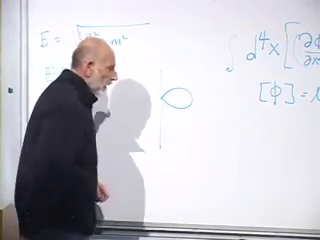
\includegraphics[width=0.72\textwidth]{lecture_03_figure_02.png}
\lectureframe{00:28:30.560}

\medskip
\begin{tikzpicture}[line width=0.8pt,scale=1.0]
  \draw[dashed] (-2.6,0) -- (0,0) -- (2.6,0);
  \fill (0,0) circle (0.055);
  \draw (0,0) .. controls (-0.85,0.7) and (-0.85,1.6) .. (0,1.6)
                .. controls (0.85,1.6) and (0.85,0.7) .. (0,0);
\end{tikzpicture}
\caption{Bảng tại thời điểm chuyển sang tự năng vô hướng, tiếp theo là bản vẽ lại sơ lược một cách dè dặt của tôpô tadpole. Ảnh chụp màn hình cho thấy chắc chắn vòng lặp, các công thức năng lượng tương đối tính và không khối lượng, cùng một phần tác dụng; các hệ số và nhãn bị che khuất không được khẳng định là nhìn thấy được.}
\end{figure}

Tại đỉnh, trường vô hướng có thể bị hấp thụ rồi phát xạ lại, trong khi hai chân còn lại truyền từ điểm đó quay về chính điểm ấy. Bỏ qua các hệ số số học và tổ hợp, hiệu chỉnh là
\begin{equation}
\delta m_\phi^2\sim \lambda G_\phi(0).
\end{equation}
Propagator tại điểm trùng là vô hạn trong gần đúng liên tục. Một lý thuyết hiệu dụng không tự nhận có hiệu lực ở khoảng cách ngắn tùy ý, nên áp đặt \(|\Delta|\geq\delta\). Khi đó
\begin{equation}
G_\phi(0)\longrightarrow G_\phi(\delta)sim\frac{1}{\delta^2},
\qquad
\delta m_\phi^2\sim\frac{\lambda}{\delta^2}sim\lambda\Lambda^2.
\end{equation}
Phân kỳ này được gọi là bậc hai vì nó chứa hai lũy thừa của cutoff xung lượng. Tích phân trong không gian xung lượng cho cùng kết luận: đóng góp quá mức đến từ xung lượng vòng lớn tùy ý. Dù thang ngắn nhất rốt cuộc được ấn định bởi đại thống nhất, hấp dẫn lượng tử hay một điều gì đó chưa từng được hình dung, chẩn đoán của lý thuyết hiệu dụng vẫn không thay đổi.

Đây là một bài toán tinh chỉnh. Nếu \(\delta\) cực kỳ nhỏ và \(\lambda\) không nhỏ đến mức phi thường, thì hiệu chỉnh bức xạ lớn hơn rất nhiều so với khối lượng bình phương của trường vô hướng quan sát được ở năng lượng thấp. Khi đó, hệ số trần và hiệu chỉnh vòng phải triệt tiêu nhau đến một số chữ số khó tin:
\begin{equation}
m_{\mathrm{physical}}^2
=m_{\mathrm{bare}}^2+\delta m_\phi^2.
\end{equation}
Propagator có khối lượng không cứu được tình hình. Ở những khoảng cách gây ra phân kỳ, \(e^{-m|\Delta|}\simeq1\). Vòng tử ngoại đã quên khối lượng từ rất lâu trước khi chạm cutoff.

\section{Thứ nguyên của fermion và propagator của chúng}

Bây giờ ta lặp lại cùng phép phân tích thứ nguyên ấy cho một fermion Dirac. Tác dụng tự do của nó là
\begin{equation}
S_\psi=\int d^4x\,
\bar\psi\left(i\gamma^\mu\partial_\mu-m\right)\psi.
\end{equation}
Các ma trận gamma là các hệ số số và không thứ nguyên. Hạng động năng chỉ chứa một đạo hàm, nên
\begin{align}
1
&=L^4[\bar\psi]L^{-1}[\psi],\\
[\psi]=[\bar\psi]&=L^{-3/2}.
\end{align}
Các lũy thừa bán nguyên không có gì đáng ngại; fermion đưa các nửa vào rất nhiều chỗ.

\begin{classroomqa}
\audiencequestion{Suy ra \([\psi]\) từ số hạng khối lượng có phải sẽ dễ hơn không? \lecturetimestamp{00:36:02}}
\lecturerresponse{Có. Số hạng khối lượng cho \(L^4L^{-1}[\bar\psi\psi]=1\), do đó \([\bar\psi\psi]=L^{-3}\) và \([\psi]=L^{-3/2}\). Phép suy ra từ hạng động năng được dùng trước vì nó vẫn có ý nghĩa trong lý thuyết không khối lượng và cho thấy vì sao khối lượng fermion xuất hiện dưới dạng \(m\), chứ không phải \(m^2\).}
\end{classroomqa}

Hai trường fermion có thứ nguyên \(L^{-3}\), vì vậy cách viết tắt gọn theo thứ nguyên trong bài giảng cho hàm truyền không khối lượng là
\begin{equation}
S(\Delta)\sim\frac{1}{|\Delta|^3}.
\end{equation}
Khôi phục cấu trúc ma trận của nó cho tử số chính xác hơn mà tính hiệp biến Lorentz đòi hỏi:
\begin{equation}
S_{ij}(\Delta)
\propto
\frac{\left(\gamma_\mu\Delta^\mu\right)_{ij}}
{\left(\Delta^2\right)^2}.
\end{equation}
Tử số bổ sung một lũy thừa chiều dài, nên mẫu số vì thế chứa bốn lũy thừa của độ tách; thứ nguyên tổng cộng vẫn là \(L^{-3}\). Cũng như với trường vô hướng, khối lượng fermion làm suy giảm hàm truyền ở độ tách lớn nhưng không làm thay đổi quy luật tỉ lệ ở khoảng cách ngắn này.

\section{Vì sao một vòng fermion kín mang dấu âm}

Bây giờ ta có thể hỏi liệu một biểu đồ fermion có thể triệt tiêu tự năng boson gây rắc rối hay không. Biểu đồ tadpole vô hướng mang dấu dương, ngoại trừ các hệ số số học dương như các lũy thừa của \(\pi\) và các hệ số tổ hợp. Một vòng fermion kín mang dấu ngược lại.

\begin{classroomqa}
\audiencequestion{Dấu trừ của vòng fermion có liên quan đến thảo luận trước đó về một phép quay trọn vòng không? \lecturetimestamp{00:40:21}}
\lecturerresponse{Nó thuộc cùng một cấu trúc dấu fermion, nhưng ở đây phép chứng minh hữu ích đi qua tính phản đối xứng dưới hoán đổi chứ không qua định hướng hình học của một vòng. Hãy cắt hai vòng, hoán đổi các hạt đồng nhất, rồi nối chúng lại. Phép hoán đổi biến hai vòng thành một và chỉ đóng góp một dấu trừ đối với fermion.}
\end{classroomqa}

Lập luận này đáng được trình bày đầy đủ. Giả sử một biểu đồ một vòng có dấu \(\sigma\), hoặc dương hoặc âm. Hai vòng đồng nhất rời nhau có dấu
\begin{equation}
\sigma^2=+1.
\end{equation}
Hãy cắt đồng thời cả hai vòng. Khi đó ta có hai hạt đồng nhất truyền giữa các chỗ cắt. Hàm sóng hai hạt thông thường của chúng là đối xứng đối với boson và phản đối xứng đối với fermion:
\begin{align}
\Psi_B(x_1,x_2)&=+\Psi_B(x_2,x_1),\\
\Psi_F(x_1,x_2)&=-\Psi_F(x_2,x_1).
\end{align}
Tính phản đối xứng này cũng giải thích nguyên lý Pauli: nếu cả hai fermion được đặt vào cùng một trạng thái, thì phép hoán vị không làm thay đổi gì về mặt vật lý nhưng lại phải đảo dấu hàm sóng, buộc nó phải bằng không.

Sau khi hoán đổi hai hạt, hãy nối lại các đường đã cắt. Về mặt tôpô, hai vòng đã trở thành một. Biên độ hai vòng trước khi hoán đổi là dương. Phép hoán đổi giữ nguyên dấu dương đối với boson và đảo dấu đối với fermion. Do đó
\begin{equation}
\begin{aligned}
\operatorname{sign}(\text{closed boson loop})&=+1,\\
\operatorname{sign}(\text{closed fermion loop})&=-1.
\end{aligned}
\end{equation}
Kết luận này là tổng quát: mỗi vòng fermion kín độc lập cung cấp một thừa số \(-1\).

\section{Vòng Yukawa}

Hãy quay lại khối lượng của trường vô hướng. Một boson không thể biến thành một fermion đơn lẻ vì tính chẵn lẻ của số fermion sẽ thay đổi. Hiệu chỉnh fermion đơn giản nhất là hạt vô hướng tách thành một cặp fermion-phản fermion, cặp này truyền quanh một vòng rồi tái hợp. Tương tác được cho bởi một ghép Yukawa,
\begin{equation}
\mathcal L_Y=-g\phi\bar\psi\psi.
\end{equation}
Đối với Higgs, các fermion có thể là quark hoặc lepton. Có hai điểm tương tác và vì thế có hai thừa số \(g\).

Biểu đồ tadpole vô hướng chỉ có một điểm, mà vị trí tổng thể của nó có thể được cố định vì bất biến tịnh tiến chỉ đơn thuần cung cấp thể tích không-thời gian. Vòng Yukawa có hai điểm. Ta có thể cố định một điểm, hoặc tương đương là cố định vị trí trung bình của chúng, nhưng phải lấy tích phân theo độ tách tương đối \(\Delta\) giữa chúng. Mỗi hàm truyền fermion đóng góp thừa số khoảng cách ngắn \(1/|\Delta|^3\), nên
\begin{equation}
\delta m_{\phi,F}^2
\sim
-g^2\int_{|\Delta|\geq\delta}d^4\Delta\,
\frac{1}{|\Delta|^6}.
\end{equation}

Sau khi đã viết hai hàm truyền, tích phân theo độ tách và hai hằng số ghép, người giảng còn hỏi cả lớp một thừa số cuối cùng. Câu trả lời là dấu trừ. Hai hàm truyền khép lại thành một vòng fermion, nên toàn bộ tích phân khoảng cách ngắn vốn dĩ dương này được nhân với \(-1\).

Phân tích thứ nguyên đã xác định được phân kỳ. Bốn lũy thừa chiều dài đến từ \(d^4\Delta\), sáu lũy thừa xuất hiện ở mẫu số, và thang chiều dài duy nhất còn lại là ngưỡng cắt:
\begin{equation}
\int_{|\Delta|\geq\delta}
\frac{d^4\Delta}{|\Delta|^6}
\sim\frac{1}{\delta^2}.
\end{equation}
Trong tọa độ xuyên tâm Euclid bốn chiều, điều này có thể được viết tường minh:
\begin{equation}
\int_{\delta}^{R}d^4\Delta\,\frac{1}{|\Delta|^6}
=2\pi^2\int_{\delta}^{R}dr\,\frac{r^3}{r^6}
=\pi^2\left(\frac{1}{\delta^2}-\frac{1}{R^2}\right).
\end{equation}
Các vết spinor và chuẩn hóa của hàm truyền làm thay đổi hệ số, chứ không làm thay đổi lũy thừa bậc hai của ngưỡng cắt.\editorialnote{Tích phân xuyên tâm là một dạng tường minh chuẩn của ước lượng theo thứ nguyên đã được thực hiện trong bài giảng. Nó được viết theo khoảng cách Euclid, nơi tính dương và phép đếm lũy thừa tử ngoại hiện ra minh bạch.}

\begin{classroomqa}
\audiencequestion{Việc đảo chiều hoặc cách chọn các cận tích phân có thể làm đổi dấu không? \lecturetimestamp{00:51:06}}
\lecturerresponse{Không. Đây không phải là một tích phân định hướng một chiều mà trong đó các cận sinh ra dấu vật lý. Nó là một tích phân trên bốn thành phần, hay gọn hơn là trên một độ đo xuyên tâm dương. Độ lớn tử ngoại của nó là dương. Đóng góp âm chỉ đến từ vòng fermion kín.}
\end{classroomqa}

\begin{classroomqa}
\audiencequestion{Hằng số ghép Yukawa \(g\) có thứ nguyên gì? \lecturetimestamp{00:51:51}}
\lecturerresponse{Nó không thứ nguyên trong bốn chiều. Vì \([\phi]=L^{-1}\) và \([\bar\psi\psi]=L^{-3}\), nên tích \(\phi\bar\psi\psi\) có thứ nguyên \(L^{-4}\), được \(d^4x\) triệt tiêu chính xác.}
\end{classroomqa}

Vì thế, hiệu chỉnh do fermion ở bậc dẫn là
\begin{equation}
\delta m_{\phi,F}^2
\sim -C_F\frac{g^2}{\delta^2}
=-C_Fg^2\Lambda^2,
\end{equation}
trong đó \(C_F>0\) chứa các hệ số số học, spin và bội số. Vòng vô hướng có dạng tương ứng
\begin{equation}
\delta m_{\phi,B}^2
\sim+C_B\frac{\lambda}{\delta^2}
=+C_B\lambda\Lambda^2.
\end{equation}
Ta vẫn chưa giải quyết được bài toán tinh chỉnh, nhưng đã tìm thấy một điều không thể thiếu: một đóng góp có cùng bậc tử ngoại và dấu ngược lại.

\section{Sự triệt tiêu đòi hỏi điều gì}

Sẽ là một ngẫu nhiên phi thường nếu các hằng số ghép không liên hệ với nhau lại tình cờ thỏa mãn
\begin{equation}
C_B\lambda=C_Fg^2
\end{equation}
với đúng độ chính xác mà một phân cấp lớn của các thang đo đòi hỏi. Bài giảng viết gọn điều này thành \(g^2=\lambda\), bỏ qua các hệ số phụ thuộc quy ước và các hệ số bội số. Một lời giải thực sự cần một cấu trúc toán học buộc quan hệ đó phải đúng, chứ không chỉ đơn thuần cho phép nó.

Đó chính là động cơ của siêu đối xứng. Siêu đối xứng liên hệ boson với fermion và ràng buộc các hằng số ghép của chúng vào những tổ hợp làm cho nhiều số hạng phân kỳ vốn nguy hiểm được triệt tiêu. Khi đó sự triệt tiêu được lặp lại trên các biểu đồ vì nó là hệ quả của một đối xứng, chứ không phải vì các tham số đã được điều chỉnh lần lượt cho từng vòng.

Sự khớp nhau của khối lượng cũng quan trọng. Nếu khối lượng boson và fermion giống hệt nhau, các hàm truyền đầy đủ của chúng có thể được ghép cặp khít nhất. Nếu các khối lượng hơi khác nhau, các kết quả hữu hạn đầy đủ không triệt tiêu chính xác, vì các hàm truyền khác nhau ở những khoảng cách cỡ bước sóng Compton của chúng. Tuy vậy, các tiệm cận khoảng cách ngắn chung của chúng vẫn có thể triệt tiêu phần phân kỳ:
\begin{equation}
\mathcal I_B(\Delta)-\mathcal I_F(\Delta)
\quad\hbox{may be finite as}\quad \Delta\to0,
\end{equation}
trong đó \(\mathcal I_B\) và \(\mathcal I_F\) ký hiệu các hàm dưới dấu tích phân đầy đủ của vòng boson và vòng fermion sau khi đã tính cả các đỉnh, tử số và các hệ số bội số. Bản thân các hàm truyền có thứ nguyên khác nhau và không phải đang bị lấy hiệu trực tiếp. Ngay cả khi các số hạng tử ngoại triệt tiêu, vẫn có thể còn lại một phần dư hữu hạn. Đây là chỗ mở ra cho siêu đối xứng gần đúng hoặc bị phá vỡ. Sự bằng nhau chính xác cho sự triệt tiêu gọn ghẽ nhất; sự phá vỡ được kiểm soát đủ tốt vẫn có thể loại bỏ thảm họa tử ngoại mà vẫn để lại sự tách khối lượng có thể quan sát được.

Vì vậy, ta đã đi tới siêu đối xứng mà vẫn chưa viết ra đại số của nó. Chuỗi lập luận đã hoàn chỉnh:
\begin{equation}
\begin{gathered}
G_\phi(\Delta)\sim \Delta^{-2},
\qquad
\delta m_{\phi,B}^2\sim+C_B\lambda\Lambda^2,\\[0.4em]
S_\psi(\Delta)\sim \Delta^{-3},
\qquad
\delta m_{\phi,F}^2\sim-C_Fg^2\Lambda^2,\\[0.4em]
\text{symmetry-enforced matching}\\
\Longrightarrow\quad
\text{quadratic divergences cancel}.
\end{gathered}
\end{equation}
Nhiệm vụ tiếp theo là hiểu nguyên lý đối xứng trừu tượng nào áp đặt những quan hệ đó và xem các ví dụ cụ thể về cách nó tác động.

\chapter{Từ đối xứng thông thường đến đại số Grassmann}

\lectureoverview{Siêu đối xứng là một đối xứng, vì vậy trước hết ta nhắc lại từ đó có nghĩa gì trong cơ học lượng tử. Một phép biến đổi vật lý được biểu diễn trên không gian Hilbert bởi một toán tử unita; các phép biến đổi liên tục được sinh ra ở bậc vô cùng bé, và các giao hoán tử của chúng mã hoá cách các phép biến đổi hợp thành. Một đối xứng đúng nghĩa bảo toàn năng lượng, điều này tương đương với việc giao hoán với Hamiltonian. Khi đó, siêu đối xứng thay đổi một giả thiết mà mọi ví dụ quen thuộc đều cùng chia sẻ: các bộ sinh của nó biến boson thành fermion và fermion thành boson. Việc xây dựng các bộ sinh như vậy tự nhiên dẫn đến các toán tử tạo và hủy, các phản giao hoán tử, và đại số Grassmann hữu hạn trong đó các đại lượng lẻ bình phương bằng không.}

\section{Đối xứng liên hệ các cấu hình khác nhau}

Một đối xứng không chỉ đơn thuần là một sự đều đặn có tính trang trí. Nó là một phép toán liên hệ một cấu hình vật lý này với một cấu hình khác. Chẳng hạn, phép phản xạ trái-phải liên hệ hai bàn tay. Nếu con người đó và các định luật của môi trường xung quanh đều có đối xứng trái-phải chính xác, thì các tính chất tương ứng của hai bàn tay sẽ trùng nhau. Tổng quát hơn, các vật thể hay trạng thái được nối với nhau bởi một đối xứng chính xác phải có chung những đại lượng vật lý mà đối xứng đó bảo toàn. Trong vật lý hạt, điều đó thường có nghĩa là các khối lượng bằng nhau; trong vật lý nguyên tử, điều đó có nghĩa là các năng lượng bằng nhau đối với các trạng thái nằm trong cùng một đa bội quay.

Mục tiêu của chúng ta là siêu đối xứng, nhưng trước hết vẫn hữu ích khi nhắc lại các đối xứng liên tục như phép quay và phép tịnh tiến. Câu hỏi liệu siêu đối xứng có phải là “liên tục” theo nghĩa thông thường hay không đã có phần gượng gạo. Các tham số vô cùng bé của nó không phải là những số thực giao hoán thông thường. Tốt nhất nên xem nó như một mở rộng phân bậc của đối xứng liên tục, và phép tính Grassmann được giới thiệu bên dưới làm cho phát biểu đó đủ chính xác cho mục đích hiện tại của ta. \editorialnote{Thuật ngữ hiện đại mô tả siêu đối xứng như một đối xứng phân bậc liên tục. Sự hạn định này giải thích lời lưu ý trong bài giảng rằng câu hỏi quen thuộc đối lập liên tục với rời rạc không áp vào siêu đối xứng một cách gọn ghẽ.}

\section{Các phép biến đổi unita trên không gian Hilbert}

Một hệ lượng tử được biểu diễn bởi một vectơ trạng thái \(\ket{\psi}\). Một phép đối xứng vật lý được biểu diễn bởi một toán tử \(U\) tác dụng lên trạng thái đó:
\begin{equation}
\ket{\psi}\longmapsto U\ket{\psi}.
\end{equation}
Đối với một phép quay trong không gian, trục và góc xác định \(U\). Nếu một trạng thái chứa các hạt ở nhiều vị trí, thì ket đã biến đổi biểu diễn tất cả chúng ở các vị trí đã quay của chúng. Một phép tịnh tiến cũng hoạt động tương tự: nó thay trạng thái bằng một trạng thái trong đó toàn bộ cấu hình đã được tịnh tiến.

\begin{classroomqa}
\audiencequestion{Vectơ trạng thái thuộc về một không gian Hilbert thường là vô hạn chiều. Ta đang quay không gian Hilbert hay không gian ba chiều thông thường? \lecturetimestamp{00:04:20}}
\lecturerresponse{Hai cách mô tả đó nói về cùng một phép toán ở những mức khác nhau. Phép biến đổi unita tác dụng lên vectơ trong không gian Hilbert và biểu diễn phép quay vật lý của cấu hình trong không gian thông thường. Nó không phải theo nghĩa đen là một phép quay ba chiều của không gian Hilbert trừu tượng; nó là sự biểu diễn ở đó của một phép quay trong không gian.}
\end{classroomqa}

Điều kiện cốt yếu là tính unita:
\begin{equation}
U^\dagger U=UU^\dagger=\mathbf 1,
\qquad
U^{-1}=U^\dagger.
\end{equation}
Điều này bảo toàn các tích vô hướng và do đó bảo toàn xác suất:
\begin{equation}
\braket{U\psi}{U\psi}
=\bra{\psi}U^\dagger U\ket{\psi}
=\braket{\psi}{\psi}.
\end{equation}

\begin{figure}[H]
\centering
\includegraphics[width=0.56\textwidth]{lecture_04_figure_02.png}
\lectureframe{00:05:56.420}
\caption{Khung bảng ban đầu chuyển từ một trạng thái đã biến đổi sang điều kiện unita. Ket và tích có dấu dagger còn nhìn thấy được, nhưng giảng viên che khuất phần tận cùng bên phải của chúng; các phương trình đầy đủ xuất hiện trong phép suy ra bên dưới.}
\end{figure}

Nói chính xác hơn, định lý Wigner cũng cho phép các đối xứng phản unita như phép đảo thời gian. Các phép biến đổi nối liên tục với phép đồng nhất, vốn là chủ đề ở đây, được biểu diễn bằng các toán tử unita. \editorialnote{Khả năng phản unita là một điều kiện kèm theo tiêu chuẩn; nó không làm thay đổi phần thảo luận của bài giảng về phép quay, phép tịnh tiến hay các bộ sinh siêu đối xứng.}

\section{Các phép biến đổi vô cùng bé và các bộ sinh}

Việc không làm gì cả được biểu diễn bởi \(U=\mathbf 1\), chứ không phải \(U=0\). Một phép biến đổi đủ nhỏ khác phép đồng nhất ở một hạng tử tuyến tính theo tham số nhỏ của nó. Đối với một phép quay qua một góc nhỏ \(\epsilon\),
\begin{equation}
U(\epsilon)=\mathbf 1+i\epsilon L+O(\epsilon^2).
\end{equation}
Tính unita ở bậc một đòi hỏi
\begin{align}
U^\dagger U
&=\left(\mathbf 1-i\epsilon L^\dagger\right)
  \left(\mathbf 1+i\epsilon L\right)+O(\epsilon^2)\\
&=\mathbf 1+i\epsilon(L-L^\dagger)+O(\epsilon^2),
\end{align}
và do đó
\begin{equation}
L^\dagger=L.
\end{equation}
Toán tử \(L\) là bộ sinh vô cùng bé.

Các phép quay cần ba bộ sinh, một cho mỗi trục độc lập:
\begin{equation}
L_x,\qquad L_y,\qquad L_z.
\end{equation}
Một phép quay quanh một trục tùy ý \(\widehat{\bm n}\) được sinh bởi
\begin{equation}
L_{\widehat{\bm n}}=\widehat{\bm n}\cdot\bm L.
\end{equation}

\begin{classroomqa}
\audiencequestion{Có thể cộng các bộ sinh cho các trục \(x\), \(y\) và \(z\) để tạo thành một phép quay quanh một trục khác không? \lecturetimestamp{00:07:50}}
\lecturerresponse{Có. Các tổ hợp tuyến tính của chúng sinh ra các phép quay quanh các trục trung gian. Ba thành phần độc lập là đủ để xây dựng mọi phép quay không gian vô cùng bé.}
\end{classroomqa}

Đối với phép quay, các bộ sinh này là các thành phần của mômen động lượng. Ký hiệu này còn hữu ích một cách tổng quát hơn vì mọi đối xứng liên tục đều được hiểu cục bộ thông qua các bộ sinh của nó.

\section{Giao hoán tử như một bảng nhân}

Các bộ sinh quay tuân theo
\begin{align}
[L_x,L_y]&=iL_z,&
[L_y,L_z]&=iL_x,&
[L_z,L_x]&=iL_y,
\end{align}
hay, viết gọn,
\begin{equation}
[L_i,L_j]=i\epsilon_{ijk}L_k.
\end{equation}
Ký hiệu Levi-Civita bằng không nếu hai chỉ số trùng nhau và bằng \(+1\) hoặc \(-1\) đối với các hoán vị chẵn hay lẻ của \(1,2,3\). Sự kiện cấu trúc quan trọng là tính khép kín: giao hoán tử của hai bộ sinh lại là một bộ sinh khác.

Vì sao một giao hoán tử lại mô tả hình học của các phép quay? Hãy thực hiện một phép quay nhỏ quanh \(x\), rồi một phép quay quanh \(y\), hoàn tác phép quay \(x\), và cuối cùng hoàn tác phép quay \(y\). Các phép toán không triệt tiêu nhau vì các phép quay quanh những trục khác nhau không giao hoán.

\begin{classroomqa}
\audiencequestion{Có thể hình dung sự không giao hoán này qua các chuyển động lăn, chúc-ngẩng và quay hướng của một chiếc máy bay không? \lecturetimestamp{00:12:36}}
\lecturerresponse{Có. Các phép quay liên tiếp quanh các trục gắn với vật cho một minh hoạ hình học trực tiếp rằng việc đổi thứ tự sẽ làm đổi phương hướng cuối cùng. Đại số bên dưới là phiên bản vô cùng bé của sự kiện quen thuộc ấy.}
\end{classroomqa}

Đặt
\begin{equation}
U_x(\epsilon)=\mathbf 1+i\epsilon L_x,
\qquad
U_y(\delta)=\mathbf 1+i\delta L_y.
\end{equation}
Vì các toán tử tác dụng lên ket từ phải sang trái, nên chuỗi đã nêu được biểu diễn bởi
\begin{equation}
\mathcal C
=U_y^{-1}(\delta)U_x^{-1}(\epsilon)
 U_y(\delta)U_x(\epsilon).
\end{equation}

\begin{classroomqa}
\audiencequestion{Tại sao có thể viết các phép hoàn tác bằng nghịch đảo thay vì bằng dagger? \lecturetimestamp{00:13:25}}
\lecturerresponse{Vì các phép biến đổi là unita: \(U^\dagger=U^{-1}\). Đối với một phép biến đổi vô cùng bé, việc lấy nghịch đảo đơn giản chỉ đảo dấu của hạng tử bậc một, \(U_x^{-1}=\mathbf 1-i\epsilon L_x+O(\epsilon^2)\).}
\end{classroomqa}

Việc nhân bốn thừa số trên bảng đã trở thành một bài tập khá sôi nổi: mọi hạng tử tuyến tính theo \(\epsilon\) hoặc \(\delta\) đều triệt tiêu, cả phòng cùng theo dõi các hạng tử hỗn hợp, và một lúc lúng túng về hệ số 2 cho thấy việc làm mất thứ tự toán tử dễ đến mức nào. Kết quả bậc hai gọn gàng là
\begin{align}
\mathcal C
&=\mathbf 1+\epsilon\delta[L_x,L_y]
  +O(\epsilon^2\delta,\epsilon\delta^2)\\
&=\mathbf 1+i\epsilon\delta L_z
  +O(\epsilon^2\delta,\epsilon\delta^2).
\end{align}
Vì vậy chuỗi khép kín để lại một phép quay nhỏ quanh \(z\) qua một góc tỉ lệ với \(\epsilon\delta\). \editorialnote{Phép nhân được trình bày cố định lại thứ tự và hệ số sau phép tính thăm dò trên lớp. Đảo ngược quy ước cho chuỗi sẽ đảo dấu nhưng không làm thay đổi kết luận rằng phép biến đổi còn dư được chi phối bởi giao hoán tử.}

\begin{classroomqa}
\audiencequestion{Nếu đổi thứ tự của các phép nghịch đảo thì tích có trở thành phép đồng nhất không? \lecturetimestamp{00:25:23}}
\lecturerresponse{Nếu mỗi phép biến đổi được đặt ngay cạnh nghịch đảo của chính nó thì từng cặp sẽ triệt tiêu. Chuỗi giao hoán tử không tầm thường cố ý tách các cặp đó ra; việc nó không rút gọn chính là thước đo của sự phụ thuộc vào thứ tự.}
\end{classroomqa}

Các tích dài hơn quả thật trở nên phức tạp hơn, nhưng chúng không chứa nguyên lý mới nào.

\begin{classroomqa}
\audiencequestion{Điều gì xảy ra khi có nhiều hơn ba bộ sinh hoặc có rất nhiều phép biến đổi nhỏ? \lecturetimestamp{00:25:34}}
\lecturerresponse{Sẽ có nhiều giao hoán tử hơn và nhiều hạng tử phải theo dõi hơn, nhưng việc biết đại số khép kín cho phép ta xác định cách kết hợp của một số tùy ý các phép biến đổi vô cùng bé. Các phép biến đổi hữu hạn có thể được ghép từ nhiều phép biến đổi nhỏ.}
\end{classroomqa}

Theo nghĩa này, đại số giao hoán tử là bảng nhân của một nhóm liên tục được viết gần phép đồng nhất.

\section{Các phép tịnh tiến hoàn chỉnh ví dụ không gian}

Các phép tịnh tiến trong không gian được sinh bởi động lượng. Với quy ước dấu dùng trong bài giảng,
\begin{equation}
\begin{aligned}
T_x(a)&=\mathbf 1+iaP_x+O(a^2),\\
T_y(b)&=\mathbf 1+ibP_y+O(b^2),
\end{aligned}
\end{equation}
trong đó \(a\) và \(b\) là các khoảng cách chứ không phải các góc.

Hai phép tịnh tiến giao hoán. Dời một điểm theo \(x\), rồi theo \(y\), hoàn tác phép tịnh tiến \(x\), rồi hoàn tác phép tịnh tiến \(y\); điểm đó trở về gốc của nó:
\begin{equation}
[P_i,P_j]=0.
\end{equation}

\begin{classroomqa}
\audiencequestion{Việc tịnh tiến hay quay một vật thể vật lý có đòi hỏi lực để bắt đầu và dừng chuyển động không? \lecturetimestamp{00:28:45}}
\lecturerresponse{Đó không phải phép toán đang được định nghĩa. Một phép biến đổi đối xứng so sánh trạng thái ban đầu với trạng thái toán học trong đó toàn bộ cấu hình đã được tịnh tiến hoặc quay. Nó không mô tả một quỹ đạo động lực học, gia tốc, hay công được thực hiện trong khi di chuyển thiết bị.}
\end{classroomqa}

Một phép quay và một phép tịnh tiến không giao hoán. Tịnh tiến một điểm, quay nó quanh gốc tọa độ, tịnh tiến ngược lại dọc theo trục ban đầu, rồi hoàn tác phép quay; điểm đó không trở về nơi nó bắt đầu. Đại số hỗn hợp là
\begin{equation}
[L_i,P_j]=i\epsilon_{ijk}P_k.
\end{equation}
Hệ thức này nói rằng bản thân động lượng biến đổi như một vectơ dưới các phép quay. Bài tập về chỉ số cụ thể ở đây kém quan trọng hơn bài học tổng quát: các phép biến đổi của không gian Euclid được mã hoá trong các giao hoán tử giữa các bộ sinh quay và tịnh tiến của chúng.

\section{Một đối xứng phải bảo toàn năng lượng}

Giờ đây ta chuyển từ sự hợp thành của các phép biến đổi sang động lực học. Nếu \(U\) thật sự là một đối xứng của một hệ, thì việc áp dụng nó không thể làm thay đổi năng lượng. Gọi \(\ket{E}\) là một trạng thái riêng năng lượng:
\begin{equation}
H\ket{E}=E\ket{E}.
\end{equation}
Ký hiệu \(E\) ở vế phải là một con số; \(\ket{E}\) là một vectơ được gắn nhãn bởi trị riêng đó.

\begin{figure}[H]
\centering
\begin{minipage}[t]{0.43\textwidth}
\centering
\includegraphics[width=\linewidth]{lecture_04_figure_03.png}
\lectureframe{00:34:38.239}
\end{minipage}
\hfill
\begin{minipage}[t]{0.50\textwidth}
\centering
\includegraphics[width=\linewidth]{lecture_04_figure_04.png}
\lectureframe{00:36:22.376}
\end{minipage}
\caption{Ket đã biến đổi \(U\ket{E}\) và phương trình trị riêng định nghĩa \(H\ket{E}=E\ket{E}\), được tách riêng trong các khung bảng kế tiếp nhau.}
\end{figure}

Nếu \(U\) là một đối xứng, thì \(U\ket{E}\) có cùng trị riêng:
\begin{equation}
HU\ket{E}=EU\ket{E}.
\end{equation}
Vì \(E\) là một đại lượng vô hướng nên nó giao hoán với \(U\), và ta có thể dùng phương trình trị riêng ban đầu:
\begin{align}
HU\ket{E}
&=EU\ket{E}\\
&=UE\ket{E}\\
&=UH\ket{E}.
\end{align}
Do đó
\begin{equation}
(HU-UH)\ket{E}=0.
\end{equation}

\begin{classroomqa}
\audiencequestion{Có thể lặp lại phép suy ra bắt đầu từ hệ thức đầu tiên của nó không? \lecturetimestamp{00:35:55}}
\lecturerresponse{Bắt đầu với \(H\ket{E}=E\ket{E}\). Tính đối xứng nói rằng \(U\ket{E}\) có cùng năng lượng, nên \(HU\ket{E}=EU\ket{E}\). Chuyển đại lượng vô hướng \(E\) qua \(U\), thay \(E\ket{E}\) bằng \(H\ket{E}\), rồi lấy hiệu. Kết quả là \((HU-UH)\ket{E}=0\).}
\end{classroomqa}

\begin{figure}[H]
\centering
\includegraphics[width=0.70\textwidth]{lecture_04_figure_05.png}
\lectureframe{00:38:51.066}
\caption{Phép suy ra đầy đủ trên bảng. Các dấu chỉ dẫn cong nối mệnh đề năng lượng bằng nhau với phép thế \(E\ket{E}=H\ket{E}\); dòng cuối là \((HU-UH)\ket{E}=0\).}
\end{figure}

Lập luận này đúng với mọi trạng thái riêng năng lượng. Giả sử các trạng thái ấy tạo thành một cơ sở đầy đủ, thì một toán tử triệt tiêu từng trạng thái trong số đó là toán tử không:
\begin{equation}
[H,U]=0.
\end{equation}
Đây là tiêu chuẩn để một phép biến đổi unita không phụ thuộc thời gian là một đối xứng của Hamiltonian.

Đối với một phép biến đổi vô cùng bé,
\begin{equation}
U(\epsilon)=\mathbf 1+i\epsilon L_i+O(\epsilon^2),
\end{equation}
phép đồng nhất vốn đã giao hoán với \(H\), nên mỗi bộ sinh phải thoả mãn
\begin{equation}
[L_i,H]=0.
\end{equation}

\begin{figure}[H]
\centering
\includegraphics[width=0.47\textwidth]{lecture_04_figure_06.png}
\lectureframe{00:42:14.296}
\caption{Tiêu chuẩn đối xứng được cô đọng trên bảng: \([U,H]=0\), tiếp theo là dạng theo bộ sinh của nó, được chuẩn hoá từ nhãn phía dưới hơi mờ thành \([L_i,H]=0\).}
\end{figure}

Nếu \(L_i\) không phụ thuộc tường minh vào thời gian, thì phương trình Heisenberg cho
\begin{equation}
\frac{dL_i}{dt}
=i[H,L_i]=0
\qquad(\hbar=1).
\end{equation}
Do đó, các bộ sinh đối xứng là các điện tích bảo toàn. Đối xứng tịnh tiến trong không gian cho bảo toàn động lượng; đối xứng quay cho bảo toàn mômen động lượng. \editorialnote{Điều kiện về đạo hàm theo thời gian tường minh là điều chuẩn và được ngầm hiểu trong phát biểu về định luật bảo toàn của bài giảng.}

\section{Biến đổi toàn bộ hệ vật lý}

Cụm từ “phép quay là một đối xứng” có thể bị dùng sai nếu chỉ biến đổi một phần của bố trí thí nghiệm. Một spin tự do có thể bị quay mà không làm thay đổi năng lượng của nó. Tuy nhiên, nếu đặt nó trong một từ trường cố định rồi chỉ quay spin, thì năng lượng Zeeman của nó thay đổi. Điều đó không bác bỏ đối xứng quay; nó có nghĩa là từ trường đã bị giữ cố định trong khi spin bị quay tương đối so với trường. Nếu quay spin và trường cùng nhau, hoặc dùng một trường ngoài mà bản thân nó bất biến, thì năng lượng không đổi.

Cùng vấn đề ấy cũng xuất hiện trong nguyên tử hydro. Chỉ tịnh tiến electron tương đối so với proton sẽ làm thay đổi khoảng cách giữa chúng và vì thế làm thay đổi năng lượng Coulomb. Đối xứng tịnh tiến tác dụng lên toàn bộ hệ electron-proton, dời cả hai đi cùng một lượng.

\begin{classroomqa}
\audiencequestion{Bản thân một trường ngoài có nhất thiết phải có đối xứng đó không? \lecturetimestamp{00:43:09}}
\lecturerresponse{Hoặc trường ngoài cố định ấy vốn đã bất biến dưới phép biến đổi đó, hoặc nó phải được biến đổi cùng với phần còn lại của hệ. Một phép quay tương đối giữa spin và một trường không bị quay là một cấu hình vật lý khác, chứ không phải phép biến đổi đối xứng của toàn bộ cách bố trí.}
\end{classroomqa}

Sự suy biến quay trong một nguyên tử cho một ví dụ khẳng định rất rõ. Với một mômen động lượng cố định \(l\), các phép quay trộn các trạng thái có các số lượng tử từ
\begin{equation}
m=-l,-l+1,\ldots,l.
\end{equation}
Khi không có từ trường hay điện trường ngoài, mọi thành viên của đa bội đều có cùng năng lượng:
\begin{equation}
E_{l,m}=E_l.
\end{equation}
Đối xứng liên hệ các trạng thái khác nhau và buộc chúng phải suy biến.

\section{Siêu đối xứng thay đổi điều gì}

Mọi đối xứng quen thuộc đã được thảo luận cho đến nay đều bảo toàn tính chất boson hay fermion. Một phép quay biến một electron thành một electron khác, chứ không thành một photon. Các phép quay màu trộn ba màu của một quark nhưng không biến quark thành gluon. Các đối xứng nội bộ và đối xứng không-thời gian thông thường có thể trộn các thành phần hay các nhãn lượng tử, nhưng các bộ sinh của chúng là bosonic và không làm thay đổi tính chẵn lẻ fermion.

Siêu đối xứng thì khác:
\begin{equation}
Q\ket{B}\sim\ket{F},
\qquad
Q\ket{F}\sim\ket{B}.
\end{equation}
Các đa bội của nó vượt qua ranh giới giữa boson và fermion. Trong một lý thuyết siêu đối xứng chính xác, các đối tác trong cùng một đa bội có cùng khối lượng. Đây chính xác là sự ghép cặp mà các bài giảng trước đòi hỏi: các vòng boson và fermion được ghép tương ứng có thể triệt tiêu các hiệu chỉnh tử ngoại lớn đối với khối lượng vô hướng. Cấu trúc ấy khó hình dung trực quan vì không có chuyển động không gian thông thường nào biến một trạng thái spin nguyên thành một trạng thái spin bán nguyên. Vì vậy ta sẽ tiến hành theo cách đại số.

\section{Một siêu tích nguyên mẫu}

Cho \(A,A^\dagger\) lần lượt hủy và tạo một boson, và cho \(C,C^\dagger\) lần lượt hủy và tạo một fermion. Toán tử Hermite đơn giản nhất hoán đổi các trạng thái một hạt của chúng là
\begin{equation}
Q=C^\dagger A+A^\dagger C.
\end{equation}
Hạng thứ nhất lấy đi một boson và tạo ra một fermion; hạng thứ hai lấy đi một fermion và tạo ra một boson. Nếu \(Q\) tác dụng lên một trạng thái một-boson, thì hạng \(A^\dagger C\) triệt tiêu vì không có fermion nào để hủy, còn \(C^\dagger A\) thực hiện phép chuyển đổi. Trên một trạng thái một-fermion thì vai trò đảo lại.

\begin{classroomqa}
\audiencequestion{Cấu trúc này có tạo ra một hạt đơn lẻ là chồng chập của một boson và một fermion không? \lecturetimestamp{00:52:37}}
\lecturerresponse{\(Q\) là một toán tử, không phải một trạng thái. Tác dụng lên một trạng thái boson thuần, nó tạo ra một trạng thái fermion, và tác dụng lên một trạng thái fermion thuần, nó tạo ra một trạng thái boson. Tác dụng tuyến tính lên một chồng chập tổng quát đã có sẵn thì nó cho ra một chồng chập khác, đúng như mọi toán tử tuyến tính vẫn làm.}
\end{classroomqa}

Tiếp đó, cả lớp xét trạng thái chân không. Vì cả hai toán tử hủy đều triệt tiêu nó,
\begin{equation}
A\ket{0}=0,\qquad C\ket{0}=0,
\end{equation}
ta có
\begin{equation}
Q\ket{0}=0.
\end{equation}
Kết quả là vectơ không, không phải một bản sao thứ hai của chân không.

Nguyên mẫu này cố ý chỉ mang tính sơ đồ. Một boson spin không có thể được ánh xạ vào một trong hai thành phần của một fermion spin một nửa, nên bản thân bộ sinh cần một chỉ số spinor:
\begin{equation}
Q_\alpha\ket{B}\sim\ket{F_\alpha}.
\end{equation}
Trong mô tả hai thành phần đơn giản hóa của bài giảng,
\begin{equation}
Q_\alpha\ket{F_\beta}\sim\delta_{\alpha\beta}\ket{B}.
\end{equation}

\begin{classroomqa}
\audiencequestion{Làm sao số chiều của không gian trạng thái có thể khớp nhau khi một boson spin không có một thành phần spin còn một fermion spin một nửa có hai? \lecturetimestamp{00:55:02}}
\lecturerresponse{Một \(Q\) đơn lẻ không có chỉ số là không đủ. Có các thành phần spinor \(Q_\alpha\), mỗi thành phần có thể tạo ra một thành phần spin của fermion. Bản thân siêu tích mang nửa đơn vị spin vì nó làm thay đổi spin đi nửa đơn vị.}
\end{classroomqa}

Các \(Q_\alpha\) là các toán tử fermionic, hay chính xác hơn là các toán tử lẻ Grassmann. Mỗi hạng trong chúng chứa một số lẻ toán tử fermion, đó là lý do chúng đảo tính chẵn lẻ fermion. Các đại lượng quan sát được thông thường là chẵn. Cần phân biệt một siêu tích lẻ với tham số biến đổi lẻ của nó: một phép biến đổi siêu đối xứng hữu hạn được xây dựng từ một tổ hợp chẵn như \(\epsilon^\alpha Q_\alpha+\bar\epsilon_{\dot\alpha}\bar Q^{\dot\alpha}\), trong đó cả \(\epsilon\) lẫn \(Q\) đều lẻ. \editorialnote{Bài giảng gọi một cách không chặt chẽ các bộ sinh là các số Grassmann. Chính xác hơn, các siêu tích là các toán tử lẻ, còn các tham số phản giao hoán là các số Grassmann; tích của chúng là chẵn và có thể xuất hiện trong một phép biến đổi hữu hạn.}

\section{Đại số toán tử bosonic và fermionic}

Đối với các mode boson được gán nhãn bởi \(i,j\),
\begin{align}
[A_i,A_j]&=0,&
[A_i^\dagger,A_j^\dagger]&=0,&
[A_i,A_j^\dagger]&=\delta_{ij}.
\end{align}
Các nhãn ấy có thể chỉ động lượng, vị trí, spin, hoặc bất kỳ cơ sở một-hạt đầy đủ nào. Vì các toán tử tạo giao hoán với nhau,
\begin{equation}
A_i^\dagger A_j^\dagger\ket{0}
=A_j^\dagger A_i^\dagger\ket{0}.
\end{equation}
Trạng thái hai boson là đối xứng dưới phép hoán đổi.

Các toán tử fermion tuân theo các quan hệ phản giao hoán:
\begin{align}
\{C_i,C_j\}&=0,&
\{C_i^\dagger,C_j^\dagger\}&=0,&
\{C_i,C_j^\dagger\}&=\delta_{ij},
\end{align}
trong đó
\begin{equation}
\{X,Y\}=XY+YX.
\end{equation}
Đối với một mode đơn,
\begin{equation}
\{C^\dagger,C^\dagger\}=2(C^\dagger)^2=0,
\end{equation}
nên
\begin{equation}
(C^\dagger)^2=0.
\end{equation}
Bản thân toán tử không bằng không; bình phương của nó mới bằng không. Nó có thể tạo ra một fermion trong mode ấy, nhưng lần tác dụng thứ hai cho ra không. Đây là nguyên lý loại trừ Pauli trong ngôn ngữ toán tử.

Với các nhãn khác nhau,
\begin{equation}
C_i^\dagger C_j^\dagger\ket{0}
=-C_j^\dagger C_i^\dagger\ket{0},
\end{equation}
đó chính là tính phản đối xứng của trạng thái hai fermion. Sự thay thế đại số
\begin{equation}
\begin{gathered}
\text{bosons: commutators}\\
\Updownarrow\\
\text{fermions: anticommutators}
\end{gathered}
\end{equation}
mã hóa sự khác biệt về thống kê.

Nhiều boson có thể chiếm cùng một mode. Vì vậy, một số chiếm photon lớn có thể ứng xử như một trường điện từ cổ điển với một biên độ số thông thường. Fermion không thể tích tụ trong một mode, và một trường fermion lẻ không nhận một giá trị cổ điển giao hoán thông thường. Điều này thúc đẩy một kiểu số học khác cho việc xử lý fermion.

\section{Số Grassmann và tính chẵn lẻ}

Các số thông thường giao hoán:
\begin{equation}
\alpha_i\alpha_j=\alpha_j\alpha_i.
\end{equation}
Các phần tử sinh Grassmann phản giao hoán:
\begin{equation}
\theta_i\theta_j=-\theta_j\theta_i.
\end{equation}
Lấy \(i=j\), trên một hệ số mà \(2\neq0\), ta được
\begin{equation}
\theta_i^2=0.
\end{equation}
Không thể gán cho \(\theta_i\) một giá trị số thông thường nào như sáu hay bảy. Những ký hiệu này tạo thành một đại số được thiết kế để theo dõi các dấu fermion.

Các hệ số thông thường giao hoán với các phần tử sinh Grassmann:
\begin{equation}
\alpha\theta_i=\theta_i\alpha.
\end{equation}

\begin{classroomqa}
\audiencequestion{Khi một số thông thường nhân với một số Grassmann thì kết quả là loại đối tượng gì? \lecturetimestamp{01:12:32}}
\lecturerresponse{Nó vẫn là lẻ Grassmann. Nhân với một hệ số thông thường làm thay đổi độ lớn của nó, chứ không làm thay đổi tính chẵn lẻ. Bao tuyến tính của các phần tử sinh là một không gian vectơ trên các số thông thường.}
\end{classroomqa}

Đại số này có tính chẵn lẻ \(\mathbb Z_2\). Các hệ số thông thường và tích của một số chẵn phần tử sinh là chẵn; một phần tử sinh hoặc tích của một số lẻ phần tử sinh là lẻ:
\begin{equation}
\begin{aligned}
\text{even}\cdot\text{even}&=\text{even},\\
\text{even}\cdot\text{odd}&=\text{odd},\\
\text{odd}\cdot\text{odd}&=\text{even}.
\end{aligned}
\end{equation}

\begin{classroomqa}
\audiencequestion{Điều này có tương tự với các quy tắc nhân của số thực và số ảo, hay là một sự khái quát hóa giống như việc đưa vào \(i\)? \lecturetimestamp{01:14:25}}
\lecturerresponse{Đó là một sự khái quát của số học, nhưng không nên đẩy phép tương tự ấy đi quá xa. Số ảo vẫn giao hoán và thỏa mãn \(i^2=-1\); các đại lượng lẻ Grassmann phản giao hoán và bình phương bằng không. Mẫu nhân chẵn-lẻ chung đó không làm cho các đại số trở nên giống hệt nhau.}
\end{classroomqa}

Một tích như \(\theta_1\theta_2\) là chẵn và giao hoán với mọi phần tử thuần nhất của đại số Grassmann, nhưng nó không phải là một số thông thường. Nó khác không trong khi
\begin{equation}
(\theta_1\theta_2)^2=0.
\end{equation}

\begin{classroomqa}
\audiencequestion{Nếu \(\theta_1\theta_2\) là chẵn, tại sao nó không đơn giản là một số thông thường? \lecturetimestamp{01:17:36}}
\lecturerresponse{Tính chẵn có nghĩa là nó giao hoán trong đại số phân bậc; điều đó không có nghĩa rằng nó là một vô hướng thực hay phức. Tính lũy linh của nó ngay lập tức phân biệt nó với một số thông thường khác không.}
\end{classroomqa}

\section{Hàm của các biến Grassmann}

Với một phần tử sinh, mọi đa thức đều dừng lại sau bậc nhất:
\begin{equation}
f(\theta)=\alpha+\beta\theta.
\end{equation}
Mọi lũy thừa \(\theta^n\) với \(n\geq2\) đều triệt tiêu. Với hai phần tử sinh, phần tử tổng quát nhất là
\begin{equation}
f(\theta_1,\theta_2)
=\alpha+\beta_1\theta_1+\beta_2\theta_2
+\gamma\theta_1\theta_2.
\end{equation}
Viết đơn thức cuối cùng theo thứ tự đảo ngược sẽ đổi dấu của nó:
\begin{equation}
\theta_2\theta_1=-\theta_1\theta_2.
\end{equation}

\begin{classroomqa}
\audiencequestion{Nhân \(\theta_1\) với một hệ số \(\beta\) có tạo ra một biến Grassmann độc lập thứ ba không? \lecturetimestamp{01:18:39}}
\lecturerresponse{Không. Nó tạo ra một vectơ khác trong bao tuyến tính của \(\theta_1\), chứ không phải một phần tử sinh cơ sở mới. Với hai phần tử sinh độc lập, mọi hạng tuyến tính lẻ đều là \(\beta_1\theta_1+\beta_2\theta_2\).}
\end{classroomqa}

Đối với ba phần tử sinh, cơ sở có thứ tự là
\begin{equation}
1,\quad
\theta_1,\theta_2,\theta_3,\quad
\theta_1\theta_2,\theta_1\theta_3,\theta_2\theta_3,\quad
\theta_1\theta_2\theta_3.
\end{equation}
Nói chung, \(n\) phần tử sinh cho ra \(2^n\) đơn thức cơ sở có thứ tự. Mọi hàm giải tích của hữu hạn phần tử sinh Grassmann đều bị cắt cụt thành một đa thức như vậy vì các phần tử sinh lặp lại đều triệt tiêu. \editorialnote{Cơ sở \(2^n\) chiều này phát biểu tường minh mẫu hình mà bài giảng xây dựng cho một, hai và ba phần tử sinh.}

\section{Phép đạo hàm Grassmann}

Đối với một biến, định nghĩa
\begin{equation}
\frac{\partial}{\partial\theta}\alpha=0,
\qquad
\frac{\partial}{\partial\theta}\theta=1,
\end{equation}
để cho
\begin{equation}
\frac{\partial}{\partial\theta}
(\alpha+\beta\theta)=\beta.
\end{equation}
Với hai biến, chọn đạo hàm trái và giữ thứ tự chuẩn tắc \(\theta_1\theta_2\):
\begin{align}
\frac{\partial^L f}{\partial\theta_1}
&=\beta_1+\gamma\theta_2,\\
\frac{\partial^L f}{\partial\theta_2}
&=\beta_2-\gamma\theta_1.
\end{align}
Dấu trừ ở dòng thứ hai xuất hiện vì đạo hàm lẻ phải đi qua \(\theta_1\) trước khi đạo hàm \(\theta_2\).

Điều này được biểu diễn bằng quy tắc tích có phân bậc. Nếu \(A\) có tính chẵn lẻ \(|A|\in\{0,1\}\), thì
\begin{equation}
\frac{\partial^L}{\partial\theta}(AB)
=\left(\frac{\partial^L A}{\partial\theta}\right)B
+(-1)^{|A|}A
\left(\frac{\partial^L B}{\partial\theta}\right).
\end{equation}
Về tinh thần, quy tắc ấy là thông thường nhưng chứa dấu mà phản giao hoán đòi hỏi. Phép tích phân Grassmann cũng có thể được định nghĩa và, vì không gian hàm là hữu hạn, quy về một bảng ngắn. Bài giảng hoãn lại bảng ấy.

\section{Câu đố về hàm mũ, được giải quyết}

Với một phần tử sinh Grassmann duy nhất và hệ số thông thường \(a\),
\begin{equation}
e^{a\theta}
=1+a\theta,
\end{equation}
vì mọi lũy thừa bậc cao hơn đều triệt tiêu. Hai hàm mũ chứa cùng một phần tử sinh tuân theo
\begin{align}
e^{a\theta}e^{b\theta}
&=(1+a\theta)(1+b\theta)\\
&=1+(a+b)\theta\\
&=e^{(a+b)\theta}.
\end{align}

Tiếp đó, cả lớp thử với các phần tử sinh khác nhau. Nhân trực tiếp cho
\begin{equation}
e^{\theta_1}e^{\theta_2}
=(1+\theta_1)(1+\theta_2)
=1+\theta_1+\theta_2+\theta_1\theta_2.
\end{equation}
Thoạt đầu, phép khai triển trên bảng gợi ý rằng bình phương của \(\theta_1+\theta_2\) có thể cung cấp hạng cuối. Một người nghe nhận ra dấu:
\begin{equation}
(\theta_1+\theta_2)^2
=\theta_1^2+\theta_1\theta_2
 +\theta_2\theta_1+\theta_2^2
=0.
\end{equation}

\begin{classroomqa}
\audiencequestion{Có phải hạng bình phương triệt tiêu vì nó chứa \(\theta_1\theta_2+\theta_2\theta_1\) không? \lecturetimestamp{01:24:00}}
\lecturerresponse{Đúng. Sự hiệu chỉnh ấy làm thay đổi kết luận: \(e^{\theta_1+\theta_2}=1+\theta_1+\theta_2\), trong khi tích theo thứ tự \(e^{\theta_1}e^{\theta_2}\) cũng chứa \(\theta_1\theta_2\). Quy luật cộng mũ ngây thơ không áp dụng cho các số mũ phản giao hoán khác nhau.}
\end{classroomqa}

Không có mâu thuẫn nào cả. Ngay cả các ma trận thông thường cũng chỉ thỏa \(e^Ae^B=e^{A+B}\) khi \(A\) và \(B\) giao hoán. Ở đây
\begin{equation}
[\theta_1,\theta_2]
=\theta_1\theta_2-\theta_2\theta_1
=2\theta_1\theta_2.
\end{equation}
Giao hoán tử này là chẵn và giao hoán với cả hai phần tử sinh, nên chuỗi Baker-Campbell-Hausdorff dừng lại:
\begin{equation}
e^{\theta_1}e^{\theta_2}
=\exp\left(
\theta_1+\theta_2+\frac12[\theta_1,\theta_2]
\right)
=e^{\theta_1+\theta_2+\theta_1\theta_2}.
\end{equation}
Vì số mũ ở vế phải là lũy linh, nó khai triển đúng thành
\(1+\theta_1+\theta_2+\theta_1\theta_2\). \editorialnote{Phép tính BCH này cung cấp lời giải mà bài giảng trực tiếp để lại như một câu hỏi. Bài giảng phát hiện đúng sự thất bại của quy luật ngây thơ nhưng kết thúc trước khi xác định hạng giao hoán tử còn thiếu.}

\begin{classroomqa}
\audiencequestion{\(1+\theta_1\) là loại số gì, và có được phép cộng phần thông thường với phần Grassmann không? \lecturetimestamp{01:26:16}}
\lecturerresponse{Nó là một phần tử không thuần nhất của đại số Grassmann, với phần chẵn \(1\) và phần lẻ \(\theta_1\). Những tổng như vậy được phép, nhưng chúng không phải là các vô hướng thông thường cũng không phải là các phần tử lẻ thuần nhất.}
\end{classroomqa}

Gần cuối, một nghịch lý bề ngoài khác được kiểm tra:
\begin{equation}
(\theta_1+\theta_2)^2=0.
\end{equation}
Điều này không hàm ý \(\theta_1\theta_2=0\), vì hai hạng chéo triệt tiêu lẫn nhau chứ không tự triệt tiêu riêng rẽ.

\begin{classroomqa}
\audiencequestion{Nếu mọi phần tử Grassmann lẻ đều có bình phương bằng không, điều đó có nghĩa là tích của bất kỳ hai bộ sinh Grassmann nào cũng bằng không không? \lecturetimestamp{01:32:19}}
\lecturerresponse{Không. Phương trình \((\theta_1+\theta_2)^2=0\) cho biết \(\theta_1\theta_2+\theta_2\theta_1=0\). Nó chứng minh tính phản giao hoán, chứ không phải rằng từng tích có thứ tự riêng rẽ đều triệt tiêu. Các bộ sinh phân biệt có thể có tích khác không.}
\end{classroomqa}

\begin{classroomqa}
\audiencequestion{Khi viết các hàm mũ này, có phải ta đang giả sử định nghĩa chuỗi lũy thừa thông thường không? \lecturetimestamp{01:34:42}}
\lecturerresponse{Vâng, và định nghĩa đó là nhất quán vì mọi chuỗi đều kết thúc. Điều không đúng không phải là bản thân hàm mũ, mà là đồng nhất thức không được biện minh \(e^Ae^B=e^{A+B}\) đối với \(A\) và \(B\) không giao hoán. Số hạng hiệu chỉnh bằng giao hoán tử khôi phục quy luật hợp thành đúng.}
\end{classroomqa}

Phần kết thúc mang tính thăm dò này là thích hợp. Các đối xứng thông thường đã đưa ta từ các phép biến đổi unita đến các bộ sinh và các giao hoán tử; siêu đối xứng đã đưa ta từ các bộ sinh lẻ đến các biến phản giao hoán. Trong cả hai trường hợp, quy luật nhân là đối tượng trung tâm. Đối với các phép quay, nó xuất hiện trong \([L_i,L_j]\); đối với các hàm mũ Grassmann, nó xuất hiện trong số hạng giao hoán tử ngăn cản phép cộng ngây thơ. Đại số này không quen thuộc, nhưng nó mạch lạc, hữu hạn, và hoàn toàn thích hợp với các phép biến đổi fermionic mà siêu đối xứng đòi hỏi.

\chapter{Siêu điện tích, tính đóng và siêu không gian}

\lectureoverview{Siêu đối xứng khó không phải vì các quy tắc của nó nhiều, mà vì các quy tắc ấy nối kết những ý niệm mà vật lý thông thường giữ tách rời. Ta bắt đầu với các biến Grassmann, mà các phần tử lẻ của chúng phản giao hoán và các hàm của chúng dừng lại sau hữu hạn hạng. Đại số đạo hàm của chúng sau đó cung cấp mô hình cho các bộ sinh đối xứng lẻ. Một dao động tử boson và một dao động tử fermion cho các siêu điện tích đơn giản nhất: phản giao hoán tử của chúng là Hamiltonian, vì vậy việc trao đổi boson và fermion gắn liền không thể tách rời với phép tịnh tiến theo thời gian. Cùng đại số đó cũng có thể được biểu diễn hình học bằng các phép tịnh tiến theo các phương Grassmann của một không-thời gian mở rộng gọi là siêu không gian.}

\section{Vì sao ta phải lùi lại trước khi tiến lên}

Siêu đối xứng là một trong những cấu trúc trừu tượng nhất của vật lý. Nó giống các phép quay và các phép tịnh tiến vì nó là một đối xứng, nhưng nó không nằm gọn trong không-thời gian thông thường nếu không mở rộng điều ta gọi là một tọa độ. Các tham số tự nhiên của nó là các đại lượng Grassmann: những đối tượng có thể cộng và nhân, nhưng phản giao hoán thay vì giao hoán.

Đó là lý do vì sao việc lao thẳng vào đại số cuối cùng sẽ không hữu ích. Trước hết ta sẽ làm cho phép tính lẻ trở nên dùng được, rồi nhắc lại cách các đối xứng liên tục thông thường được tổ chức, và chỉ sau đó mới kết hợp hai ý tưởng ấy. Lộ trình này dài hơn, nhưng mỗi bước đều chuẩn bị cho bước tiếp theo.

\section{Dạng thao tác của đại số Grassmann}

\subsection{Phần tử lẻ và phần tử chẵn}

Hãy để \(\epsilon_i\) ký hiệu các bộ sinh Grassmann độc lập. Chúng thỏa mãn
\begin{equation}
\epsilon_i\epsilon_j=-\epsilon_j\epsilon_i,
\qquad
\{\epsilon_i,\epsilon_j\}=0.
\end{equation}
Đặt \(i=j\), ta được
\begin{equation}
2\epsilon_i^2=0,
\qquad
\epsilon_i^2=0,
\end{equation}
trên trường số thực hoặc số phức. Bộ sinh không bằng không; chỉ có bình phương của nó bằng không.

Mỗi phần tử thuần nhất có một độ chẵn lẻ. Một tích chứa số lẻ các bộ sinh Grassmann là lẻ, còn một tích chứa số chẵn bộ sinh là chẵn:
\begin{align}
\text{odd}\times\text{odd}&=\text{even},\\
\text{odd}\times\text{even}&=\text{odd},\\
\text{even}\times\text{even}&=\text{even}.
\end{align}
Các phần tử chẵn giao hoán với các phần tử thuần nhất. Hai phần tử lẻ phản giao hoán. Do đó
\begin{equation}
n\epsilon_i=\epsilon_i n,
\qquad
\epsilon_i\epsilon_j=-\epsilon_j\epsilon_i,
\end{equation}
khi \(n\) là chẵn.

Một phần tử chẵn không nhất thiết là một số thực hay số phức thông thường. Chẳng hạn, tích \(\epsilon_1\epsilon_2\) là chẵn và lũy linh. Các số thông thường tạo thành phần vô hướng của đại số, còn các tích chẵn cung cấp thêm những phần tử giao hoán.

\begin{classroomqa}
\audiencequestion{Có sự phân biệt nào giữa đại số Grassmann và các số Grassmann không, hay chúng là cùng một thứ? \lecturetimestamp{00:06:45}}
\lecturerresponse{Các phần tử là các số Grassmann; còn đại số là tập hợp các phần tử ấy cùng với các quy tắc cộng và nhân của chúng. Vì thế ta có thể nói một cách lỏng là cùng một đối tượng, nhưng vẫn hữu ích khi phân biệt những thứ đang được thao tác với các quy tắc chi phối các thao tác ấy.}
\end{classroomqa}

\subsection{Các hàm dừng lại}

Một hàm của một biến Grassmann chỉ có hai lũy thừa khả dĩ:
\begin{equation}
f(\epsilon)=a+b\epsilon.
\end{equation}
Không có hạng \(\epsilon^2\). Với hai bộ sinh độc lập,
\begin{equation}
f(\epsilon_1,\epsilon_2)
=a+b_1\epsilon_1+b_2\epsilon_2+c\epsilon_1\epsilon_2.
\end{equation}
Khai triển dừng lại sau khi cả hai bộ sinh đã xuất hiện. Với \(n\) bộ sinh độc lập, các đơn thức có thứ tự tạo thành một cơ sở \(2^n\) chiều:
\begin{equation}
1,\quad
\epsilon_i,\quad
\epsilon_i\epsilon_j,\quad
\ldots,\quad
\epsilon_1\epsilon_2\cdots\epsilon_n.
\end{equation}
\editorialnote{Phát biểu hữu hạn chiều \(2^n\) là khuôn mẫu tổng quát đứng sau các ví dụ một và hai bộ sinh. Cũng có thể định nghĩa một đại số Grassmann vô hạn, nhưng mọi đa thức dùng ở đây đều chỉ liên quan đến hữu hạn bộ sinh.}

Khi hai bộ sinh thực được ghép thành một cặp phức \(\theta,\bar\theta\), với một quy ước thứ tự đã chọn, một hàm tổng quát có thể viết thành
\begin{equation}
f(\theta,\bar\theta)
=a+\bar b\,\theta+\bar\theta\,b+c\,\bar\theta\theta.
\end{equation}
Dấu gạch trên biểu thị ký hiệu cặp phức dùng ở đây. Đảo thứ tự ở hạng cuối làm đổi dấu:
\begin{equation}
\bar\theta\theta=-\theta\bar\theta.
\end{equation}

Thường sẽ thuận tiện nếu gán cho toàn bộ hàm một độ chẵn lẻ xác định. Nếu \(f\) là chẵn, thì \(a\) và \(c\) là chẵn, còn \(b\) và \(\bar b\) là lẻ. Nếu \(f\) là lẻ, các gán đó đảo lại. Bản thân các hệ số cũng có thể thuộc về một đại số Grassmann lớn hơn, miễn là chúng không phụ thuộc vào chính những biến mà theo đó ta đang khai triển.

\begin{classroomqa}
\audiencequestion{Có thể đưa một biến Grassmann vào các hàm lượng giác hay các hàm giải tích khác không? \lecturetimestamp{00:11:06}}
\lecturerresponse{Có, nhưng chuỗi lũy thừa dừng lại ngay lập tức. Với một bộ sinh lẻ,
\[
\sin\epsilon=\epsilon,\qquad
\cos\epsilon=1,\qquad
e^\epsilon=1+\epsilon.
\]
Tên gọi quen thuộc vẫn giữ nguyên, nhưng có quá ít lũy thừa để các hàm ấy phát triển độ phức tạp giải tích thường thấy của chúng.}
\end{classroomqa}

\section{Phép đạo hàm là việc theo dõi dấu}

Ta dùng đạo hàm Grassmann trái. Các quy tắc cục bộ xác định của nó là
\begin{equation}
\partial_\theta a=0,
\qquad
\partial_\theta(\theta B)=B,
\end{equation}
khi \(a\) và \(B\) độc lập với \(\theta\). Trước khi lấy đạo hàm, hãy chuyển \(\theta\) tương ứng sang bên trái. Mỗi lần đi qua một thừa số lẻ khác thì dấu đổi.

Chẳng hạn, nếu \(b\) là lẻ,
\begin{equation}
b\theta=-\theta b,
\qquad
\partial_\theta(b\theta)=-b.
\end{equation}
Không có điều gì bí ẩn xảy ra với đạo hàm. Dấu trừ xuất hiện trước khi lấy đạo hàm, khi các thừa số lẻ được sắp lại thứ tự.

\subsection{Phép tính hai biến}

Quay lại
\begin{equation}
f(\theta,\bar\theta)
=a+\bar b\,\theta+\bar\theta\,b+c\,\bar\theta\theta.
\end{equation}
Trước hết giả sử \(f\) là chẵn. Khi đó \(\bar b\) là lẻ và \(c\) là chẵn. Sắp lại thứ tự các hạng có chứa \(\theta\),
\begin{align}
\bar b\,\theta&=-\theta\bar b,\\
c\,\bar\theta\theta&=-\theta c\,\bar\theta.
\end{align}
Do đó
\begin{equation}
\partial_\theta f=-\bar b-c\bar\theta.
\end{equation}

Nếu \(f\) là lẻ, thì \(\bar b\) là chẵn và \(c\) là lẻ. Hạng đầu không đi qua hệ số lẻ nào, còn \(\theta\) ở hạng cuối đi qua hai thừa số lẻ, \(c\) và \(\bar\theta\). Hai dấu triệt tiêu nhau:
\begin{equation}
\partial_\theta f=\bar b+c\bar\theta.
\end{equation}

\begin{classroomqa}
\audiencequestion{Vì sao trong ví dụ chẵn, cả hai hạng còn lại đều mang dấu trừ? \lecturetimestamp{00:16:49}}
\lecturerresponse{Dấu thứ nhất xuất phát từ việc chuyển \(\theta\) qua hệ số lẻ \(\bar b\). Ở hạng cuối, \(c\) là chẵn, nhưng \(\theta\) phải đi qua biến lẻ \(\bar\theta\). Mỗi lần sắp lại như vậy đều đi qua một thừa số lẻ, nên mỗi lần đều sinh ra một dấu trừ.}
\end{classroomqa}

Câu trả lời phụ thuộc vào quy ước thứ tự, nhưng toán học thì không. Nếu ta bắt đầu từ \(c\theta\bar\theta\) thay vì \(c\bar\theta\theta\), hệ số được viết ra sẽ khác nhau bởi một dấu và công thức đạo hàm cũng sẽ thay đổi tương ứng.

\begin{classroomqa}
\audiencequestion{Hạng cuối có thể được viết với \(\theta\) và \(\bar\theta\) theo thứ tự đảo lại không, và dấu xuất hiện khi đó có ý nghĩa sâu hơn nào không? \lecturetimestamp{00:18:50}}
\lecturerresponse{Có thể viết theo một trong hai thứ tự, nhưng hoán đổi hai biến lẻ làm đổi dấu. Ta có thể hấp thụ dấu ấy vào hệ số \(c\). Ở giai đoạn này, hiệu ứng đó chỉ là chuyện ghi sổ: thứ tự có ý nghĩa, độ chẵn lẻ không đổi, và việc đổi dấu không bao giờ biến một đối tượng lẻ thành một đối tượng chẵn. Ý nghĩa vật lý xuất hiện khi chính việc ghi sổ ấy áp đặt thống kê fermion và siêu đối xứng.}
\end{classroomqa}

\begin{classroomqa}
\audiencequestion{Các hệ số \(a,b,c\) có đơn giản chỉ lấy từ trường số phức không? \lecturetimestamp{00:20:47}}
\lecturerresponse{Chúng có thể là các số phức thông thường khi độ chẵn lẻ mà chúng cần có là chẵn, nhưng chúng cũng có thể chứa các bộ sinh khác ngoài \(\theta,\bar\theta\). Đại số được quan tâm ở đây thông thường chứa mọi vô hướng phức cùng với một tập các bộ sinh lẻ được chọn và các tích của chúng.}
\end{classroomqa}

\begin{classroomqa}
\audiencequestion{Đạo hàm của các hàm chẵn và lẻ trông như đối nhau. Có phải đó là một đối xứng tổng quát không? \lecturetimestamp{00:22:31}}
\lecturerresponse{Không, tự nó không phải vậy. Các dấu xuất hiện một cách cơ học từ độ chẵn lẻ của từng hệ số và số thừa số lẻ bị đi qua. Đôi khi hai đáp án tình cờ đối nhau, nhưng quy tắc đáng tin cậy thì đơn giản hơn: mỗi lần trao đổi hai đối tượng lẻ đều đóng góp một dấu trừ.}
\end{classroomqa}

\subsection{Tọa độ và đạo hàm như các toán tử}

Có một phép tương tự thông thường rất gợi mở. Hãy để phép nhân với \(x\) và phép đạo hàm theo \(x\) tác dụng lên một hàm tùy ý \(g(x)\). Khi đó
\begin{align}
\partial_x\!\left(xg\right)&=g+xg',\\
x\partial_xg&=xg',
\end{align}
nên
\begin{equation}
[\partial_x,x]g=g.
\end{equation}
Vì điều này đúng với mọi \(g\),
\begin{equation}
[\partial_x,x]=1.
\end{equation}
Với \(p=-i\partial_x\), đây là đại số vị trí-xung lượng quen thuộc, trong hệ đơn vị \(\hbar=1\).

Phép tương tự Grassmann dùng một phản giao hoán tử. Lấy
\begin{equation}
f(\theta)=a+\theta b,
\end{equation}
với \(a\) chẵn và \(b\) lẻ, để \(f\) là chẵn. Trước hết,
\begin{equation}
\theta\partial_\theta f=\theta b.
\end{equation}
Theo thứ tự ngược lại,
\begin{align}
\partial_\theta(\theta f)
&=\partial_\theta(\theta a+\theta^2b)\\
&=a.
\end{align}
Cộng hai thứ tự lại cho chính hàm ban đầu:
\begin{equation}
\left(\partial_\theta\theta+\theta\partial_\theta\right)f
=a+\theta b=f.
\end{equation}
Do đó
\begin{equation}
\boxed{\{\partial_\theta,\theta\}=1.}
\end{equation}
Bản thân đạo hàm \(\partial_\theta\) là lẻ. Đó là lý do vì sao quan hệ chính tắc của nó với tọa độ lẻ là một phản giao hoán tử.

\begin{classroomqa}
\audiencequestion{Có thể dùng một hàm chứa cả phần chẵn lẫn phần lẻ thay vì gán một độ chẵn lẻ xác định không? \lecturetimestamp{00:31:05}}
\lecturerresponse{Có thể tạo ra những phần tử không thuần nhất như vậy, nhưng các phép tính thông thường được tổ chức theo các đối tượng thuần nhất chẵn và lẻ. Một độ chẵn lẻ xác định làm cho mọi dấu trong một tích có phân bậc đều không mơ hồ; một đối tượng trộn được xử lý bằng cách tách nó thành phần chẵn và phần lẻ.}
\end{classroomqa}

\begin{classroomqa}
\audiencequestion{Trong phép tính giao hoán tử thông thường, hàm thử \(g(x)\) có được giả sử là lẻ không? \lecturetimestamp{00:31:45}}
\lecturerresponse{Không. Đó là một hàm thông thường của một tọa độ giao hoán thông thường. Nó chỉ được đưa vào để chỉ ra cách chứng minh đồng nhất thức toán tử \([\partial_x,x]=1\) trước khi lặp lại lập luận với cặp Grassmann \(\partial_\theta,\theta\).}
\end{classroomqa}

\begin{classroomqa}
\audiencequestion{Có giới hạn nào cho số bộ sinh Grassmann độc lập không? \lecturetimestamp{00:32:16}}
\lecturerresponse{Không có giới hạn trên về mặt đại số. Với \(n\) bộ sinh, cơ sở có \(2^n\) đơn thức, nên phần ghi sổ tăng rất nhanh, nhưng bản thân phép xây dựng vẫn hoạt động với mọi \(n\) hữu hạn.}
\end{classroomqa}

\subsection{Phép tích phân}

Tích phân trên một biến Grassmann được xác định bởi
\begin{equation}
\int d\theta\,1=0,
\qquad
\int d\theta\,\theta=1.
\end{equation}
Do đó, với \(f(\theta)=a+\theta b\),
\begin{equation}
\int d\theta\,f(\theta)=b=\partial_\theta f(\theta).
\end{equation}
Vì vậy phép tích phân và phép đạo hàm thực hiện cùng một phép trích xuất thành phần. Đây là tích phân Berezin. Chuẩn hóa của nó là lựa chọn đơn giản duy nhất tương thích với bất biến tịnh tiến và phép tích phân từng phần Grassmann. \editorialnote{Các quy tắc thành phần diễn đạt chính xác nhận định của bài giảng rằng tích phân và đạo hàm Grassmann là cùng một phép toán.}

\section{Đối xứng thông thường làm mốc chuẩn}

Xét một nhóm unita liên tục với các bộ sinh Hermite \(G_i\). Gần phần tử đơn vị,
\begin{equation}
U(\alpha)=\mathbf 1+i\alpha^iG_i+O(\alpha^2),
\end{equation}
trong đó \(\alpha^i\) là các tham số giao hoán thông thường. Quy luật nhân vô cùng bé được mã hóa bởi đại số Lie
\begin{equation}
[G_i,G_j]=i f_{ij}{}^{k}G_k.
\end{equation}
Các hằng số \(f_{ij}{}^k\) là các hằng số cấu trúc. Tính đóng nghĩa là giao hoán hai bộ sinh bất kỳ sẽ cho lại một tổ hợp tuyến tính của các bộ sinh đã có trong đại số.

Đối với các phép quay,
\begin{equation}
[L_i,L_j]=i\varepsilon_{ijk}L_k.
\end{equation}
Ba thành phần Hermite có thể được kết hợp thành các toán tử bậc thang không Hermite
\begin{equation}
L_\pm=L_x\pm iL_y,
\end{equation}
chúng nâng hoặc hạ số lượng tử từ \(m\) đi một đơn vị. Các tổ hợp phức vẫn hữu ích mà không làm thay đổi tính Hermite của các bộ sinh vật lý nền tảng.

Trong một cơ sở tổng quát, chỉ hai chỉ số đầu của \(f_{ij}{}^k\) buộc phải phản đối xứng. Với một đại số compact có metric trực chuẩn bất biến, ta có thể hạ chỉ số cuối và chọn các quy ước sao cho \(f_{ijk}\) là phản đối xứng hoàn toàn, như trong trường hợp phép quay. \editorialnote{Lưu ý này tách biệt tính phản đối xứng phổ quát của giao hoán tử với tính chất mạnh hơn có được trong cơ sở quay quen thuộc.}

Để \(G_i\) sinh ra một đối xứng thực sự của một hệ không phụ thuộc thời gian,
\begin{equation}
[H,G_i]=0.
\end{equation}
Tương đương, \(G_i\) ánh xạ mọi không gian riêng của năng lượng vào chính nó. Khi không có phụ thuộc thời gian tường minh, phương trình Heisenberg cho
\begin{equation}
\frac{dG_i}{dt}=i[H,G_i]=0,
\end{equation}
vì thế bộ sinh là một điện tích bảo toàn.

Các đại lượng quan sát thông thường là chẵn. Một trường fermion là lẻ, nhưng một trường lẻ cô lập tự nó không phải là một đại lượng quan sát đo được; các toán tử vật lý chứa tổng số chẵn các thừa số fermion. Siêu đối xứng làm thay đổi độ chẵn lẻ của các bộ sinh, chứ không thay đổi độ chẵn lẻ mà các kết quả quan sát được phải có.

Ký hiệu gọn gàng cho mọi trường hợp là giao hoán tử phân bậc
\begin{equation}
[X,Y]_{\mathrm{gr}}
=XY-(-1)^{|X||Y|}YX.
\end{equation}
Nó là giao hoán tử thông thường nếu một trong hai toán tử là chẵn, và là phản giao hoán tử nếu cả hai đều lẻ.

\section{Dao động tử siêu đối xứng nhỏ nhất}

\subsection{Một mode boson và một mode fermion}

Xét một mode boson đơn với các toán tử tạo và hủy \(a_+\) và \(a_-\):
\begin{equation}
[a_-,a_+]=1,
\qquad
[a_+,a_+]=[a_-,a_-]=0.
\end{equation}
Toán tử số của nó là
\begin{equation}
N_B=a_+a_-,
\end{equation}
và số chiếm cứ của nó có thể là \(0,1,2,\ldots\).

Đối với một mode fermion đơn, đưa vào \(c_+\) và \(c_-\):
\begin{equation}
\{c_-,c_+\}=1,
\qquad
\{c_+,c_+\}=\{c_-,c_-\}=0.
\end{equation}
Do đó
\begin{equation}
c_+^2=c_-^2=0,
\qquad
N_F=c_+c_-,
\end{equation}
và số chiếm cứ chỉ có thể là \(0\) hoặc \(1\). Các toán tử boson là chẵn, các toán tử fermion là lẻ, và mọi \(a_\pm\) đều giao hoán với mọi \(c_\pm\).

\editorialnote{Tính lũy linh này giới hạn mode fermion vào một trạng thái chiếm cứ. Mode boson có số chiếm cứ không bị hạn chế; một câu nói thoáng qua theo chiều ngược lại trong phần thảo luận trên lớp được chính đại số dao động tử giải quyết.}

Giả sử boson và fermion có cùng năng lượng nghỉ \(m\), và định nghĩa
\begin{equation}
Q=\sqrt m\,a_+c_-,
\qquad
\bar Q=Q^\dagger=\sqrt m\,a_-c_+.
\end{equation}
Toán tử \(Q\) hủy một fermion và tạo một boson. Liên hợp của nó hủy một boson và tạo một fermion. Mỗi toán tử chứa một toán tử fermion và vì thế là lẻ.

Trên các trạng thái số, tác dụng của chúng được viết tường minh:
\begin{align}
Q\ket{n,1}
&=\sqrt{m(n+1)}\,\ket{n+1,0},
&
Q\ket{n,0}&=0,\\
\bar Q\ket{n,0}
&=\sqrt{mn}\,\ket{n-1,1},
&
\bar Q\ket{n,1}&=0.
\end{align}
\editorialnote{Các công thức trạng thái số là dạng chuẩn hóa trực tiếp của tác dụng thay thế hạt được mô tả trong bài giảng.}

\subsection{Phản giao hoán tử khép kín trên năng lượng}

Phiên bản phân bậc tương ứng với việc tìm một đại số Lie là tính
\begin{align}
\{Q,\bar Q\}
&=Q\bar Q+\bar Q Q\\
&=m\left(a_+c_-a_-c_+
        +a_-c_+a_+c_-\right).
\end{align}
Vì các \(a\) là chẵn, chúng đi qua các \(c\) mà không sinh dấu:
\begin{equation}
\{Q,\bar Q\}
=m\left(a_+a_-c_-c_+
        +a_-a_+c_+c_-\right).
\end{equation}
Bây giờ dùng
\begin{equation}
c_-c_+=1-c_+c_-,
\qquad
a_-a_+=a_+a_-+1.
\end{equation}
Khi đó
\begin{align}
\{Q,\bar Q\}
&=m\left[
N_B(1-N_F)+(N_B+1)N_F
\right]\\
&=m(N_B+N_F).
\end{align}
Hệ số 2 phụ thêm tạm thời xuất hiện trong lúc sắp xếp lại trực tiếp sẽ biến mất: một đóng góp cho \(N_B\), đóng góp kia cho \(N_F\).

Đối với các hạt đứng yên có cùng khối lượng, Hamiltonian là
\begin{equation}
H=m(N_B+N_F).
\end{equation}
Do đó
\begin{equation}
\boxed{\{Q,\bar Q\}=H.}
\end{equation}

\begin{figure}[H]
\centering
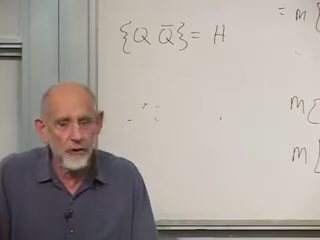
\includegraphics[width=0.62\textwidth]{lecture_05_figure_02.png}
\lectureframe{00:55:46.300}
\caption{Hệ thức khép kín trung tâm được tách riêng trên bảng. Có thể nhìn thấy các dấu ngoặc nhọn và \(Q,\bar Q,H\); dấu phẩy được bổ sung bởi ký hiệu phản giao hoán tử chuẩn.}
\end{figure}

Mốc 0 của năng lượng đã được chọn sao cho trạng thái rỗng có \(H=0\). Trong dao động tử siêu đối xứng, đây là quy ước tự nhiên: các đóng góp năng lượng không điểm của boson và fermion triệt tiêu nhau. \editorialnote{Bài giảng làm việc trực tiếp với tổng năng lượng nghỉ và không viết riêng các hạng không điểm; quy ước đã nêu làm cho lựa chọn đó trở nên tường minh.}

Hamiltonian là chẵn. Nó cũng là một bộ sinh đối xứng: nó sinh ra các phép tịnh tiến theo thời gian. Vì vậy, các bộ sinh lẻ không khép kín chỉ giữa chúng với nhau trừ phi bộ sinh chẵn của phép tịnh tiến thời gian được bao gồm.

\begin{classroomqa}
\audiencequestion{Vế nào của hệ thức là chẵn? Có phải Hamiltonian không? \lecturetimestamp{00:58:24}}
\lecturerresponse{Đúng. Năng lượng là một đại lượng quan sát thông thường, nên \(H\) là chẵn. Siêu điện tích \(Q\) là lẻ, và tích của hai đại lượng lẻ là chẵn; do đó \(\{Q,\bar Q\}\) có thể bằng \(H\). Một bộ sinh lẻ và một bộ sinh chẵn liên hệ với nhau bằng giao hoán tử, không phải phản giao hoán tử.}
\end{classroomqa}

\subsection{Hoàn tất đại số}

Các hệ thức cùng chẵn lẻ suy ra ngay:
\begin{equation}
\{Q,Q\}=2Q^2=0,
\qquad
\{\bar Q,\bar Q\}=2\bar Q^2=0,
\end{equation}
vì \(Q^2\) chứa \(c_-^2\) và \(\bar Q^2\) chứa \(c_+^2\).

Điều còn lại là hệ thức với \(H\). Đặt
\begin{equation}
H\ket{E}=E\ket{E}.
\end{equation}
Nếu khối lượng của boson và fermion bằng nhau, \(Q\) thay hạt này bằng hạt kia mà không đổi năng lượng. Do đó \(Q\ket{E}\) bằng không hoặc là một trạng thái riêng khác với cùng trị riêng:
\begin{equation}
H Q\ket{E}=E Q\ket{E}.
\end{equation}
Mặt khác,
\begin{equation}
QH\ket{E}=Q(E\ket{E})=E Q\ket{E}.
\end{equation}
Lấy hiệu,
\begin{equation}
[H,Q]\ket{E}=0.
\end{equation}
Nếu các trạng thái riêng năng lượng tạo thành một cơ sở đầy đủ, thì điều này đúng như một đồng nhất thức toán tử:
\begin{equation}
[H,Q]=0,
\qquad
[H,\bar Q]=0.
\end{equation}

\begin{classroomqa}
\audiencequestion{Điều gì xảy ra nếu boson và fermion không có cùng khối lượng? \lecturetimestamp{01:01:16}}
\lecturerresponse{Khi đó việc thay hạt này bằng hạt kia làm đổi năng lượng, nên siêu điện tích được đề xuất không giao hoán với Hamiltonian và siêu đối xứng đơn giản bị mất. Với
\[
H=m_BN_B+m_FN_F,
\]
kết quả tường minh là
\[
[H,Q]=(m_B-m_F)Q.
\]
Nó triệt tiêu đúng khi \(m_B=m_F\). \editorialnote{Giao hoán tử trong trường hợp khối lượng không bằng nhau là dạng toán tử trực tiếp của lập luận thay đổi năng lượng và làm cho điều kiện khối lượng bằng nhau trở nên tường minh.}}
\end{classroomqa}

\begin{classroomqa}
\audiencequestion{Có thể lặp lại chậm hơn lập luận dùng trạng thái riêng năng lượng không? \lecturetimestamp{01:01:37}}
\lecturerresponse{Bắt đầu với \(H\ket{E}=E\ket{E}\). Khối lượng bằng nhau ngụ ý rằng \(Q\ket{E}\) có cùng năng lượng xác định \(E\), nên \(HQ\ket{E}=EQ\ket{E}\). Theo thứ tự kia ta được \(QH\ket{E}=QE\ket{E}=EQ\ket{E}\), vì \(E\) là một vô hướng thông thường. Hiệu của chúng triệt tiêu trên mọi trạng thái riêng năng lượng. Tính đầy đủ khi đó nâng phát biểu từ các trạng thái ấy lên phương trình toán tử \([H,Q]=0\).}
\end{classroomqa}

Vì thế, đại số mô hình đồ chơi đầy đủ là
\begin{align}
\{Q,\bar Q\}&=H,\\
\{Q,Q\}&=\{\bar Q,\bar Q\}=0,\\
[H,Q]&=[H,\bar Q]=0.
\end{align}
Các siêu điện tích là những điện tích lẻ bảo toàn. Điều đáng ngạc nhiên hơn là đại số của chúng trộn một phép toán làm đổi loại hạt với bộ sinh của phép tịnh tiến trong không-thời gian.

\section{Vì sao Hamiltonian tương ứng với phép tịnh tiến theo thời gian}

Trong mô hình rút gọn này không có tọa độ không gian, nhưng có thời gian. Phương trình Schrödinger là
\begin{equation}
i\frac{\partial}{\partial t}\ket{\psi(t)}
=H\ket{\psi(t)}.
\end{equation}

\begin{figure}[H]
\centering
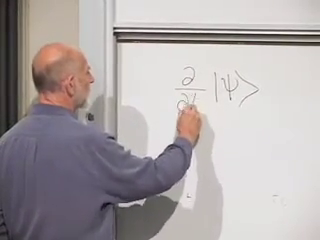
\includegraphics[width=0.56\textwidth]{lecture_05_figure_03.png}
\lectureframe{01:07:26.300}
\caption{Đạo hàm theo thời gian được viết bên cạnh \(\ket{\psi}\). Bàn tay che khuất một phần mẫu số; phương trình Schrödinger đầy đủ đã được cho ở trên.}
\end{figure}

Đối với một độ dời hữu hạn \(\delta\),
\begin{equation}
\ket{\psi(t+\delta)}
=e^{-iH\delta}\ket{\psi(t)}.
\end{equation}
Khai triển đến bậc nhất,
\begin{equation}
\ket{\psi(t+\delta)}
=\left(\mathbf 1-i\delta H\right)\ket{\psi(t)}
+O(\delta^2).
\end{equation}
Vì vậy \(H\) là bộ sinh vô cùng bé làm tiến hóa một trạng thái theo thời gian.

Các đối xứng nội tại như isospin và màu cũng làm đổi nhãn hạt. Isospin có thể trộn các trạng thái proton và neutron; các phép quay màu trộn các quark đỏ, lục và lam. Tuy vậy, không một hợp thành nào của các biến đổi nội tại ấy tịnh tiến một hệ trong không gian hay thời gian. Siêu đối xứng thì khác:
\begin{equation}
\begin{gathered}
\text{odd particle-changing transformation}\\
\mathrel{\stackrel{\{\ ,\ \}}{\Longrightarrow}}\\
\text{time translation}
\end{gathered}
\end{equation}
Đó là đầu mối cho thấy bản thân các bộ sinh lẻ có thể là các phép tịnh tiến, nhưng dọc theo những tọa độ khác với các tọa độ thông thường.

\section{Siêu không gian}

\subsection{Một hàm của thời gian và các tọa độ lẻ}

Đưa vào một hàm
\begin{equation}
\Psi=\Psi(\theta,\bar\theta,t).
\end{equation}
Nó có thể được xem như một hàm sóng trong mô hình đồ chơi hoặc, tổng quát hơn, như một siêu trường. Vì khai triển theo các biến lẻ kết thúc hữu hạn,
\begin{equation}
\Psi(\theta,\bar\theta,t)
=A(t)+\bar\chi(t)\theta
+\bar\theta\chi(t)+F(t)\bar\theta\theta.
\end{equation}
Đối tượng duy nhất này chứa gộp các hàm thành phần chẵn và lẻ. \editorialnote{Khai triển theo thành phần này áp dụng đa thức Grassmann đã được xây dựng trước đó; đó là nội dung tường minh chuẩn của một hàm trên siêu không gian đồ chơi này.}

Một phép tịnh tiến thời gian thông thường giữ \(\theta,\bar\theta\) cố định và biến
\begin{equation}
t\longmapsto t+\delta.
\end{equation}
Đến bậc nhất,
\begin{equation}
\Psi(\theta,\bar\theta,t+\delta)
=\Psi(\theta,\bar\theta,t)
+\delta\,\partial_t\Psi(\theta,\bar\theta,t).
\end{equation}

\begin{figure}[H]
\centering
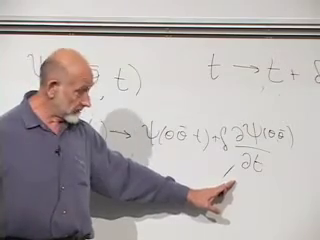
\includegraphics[width=0.72\textwidth]{lecture_05_figure_04.png}
\lectureframe{01:13:15.060}
\caption{Trên bảng, \(t\to t+\delta\) được đặt phía trên biến thiên bậc nhất của \(\Psi\), với hạng đạo hàm được chỉ ra trực tiếp.}
\end{figure}

\subsection{Tịnh tiến theo một hướng lẻ}

Bây giờ hãy nghĩ ra một phép biến đổi dịch một tọa độ lẻ:
\begin{equation}
\theta\longmapsto\theta+\epsilon,
\end{equation}
trong đó \(\epsilon\) là một tham số Grassmann lẻ khác. Đồng thời, cho thời gian nhận một độ dời lũy linh chẵn,
\begin{equation}
t\longmapsto t+i\bar\theta\epsilon.
\end{equation}
Cả \(\bar\theta\) lẫn \(\epsilon\) đều lẻ, nên tích của chúng là chẵn và có thể được cộng một cách nhất quán vào tọa độ chẵn \(t\).

Khi đưa tham số sang bên trái,
\begin{equation}
i\bar\theta\epsilon=-i\epsilon\bar\theta.
\end{equation}
Vì vậy biến thiên cảm sinh là
\begin{align}
\delta_\epsilon\Psi
&=\epsilon\,\partial_\theta\Psi
-i\epsilon\bar\theta\,\partial_t\Psi\\
&=\epsilon q_0\Psi,
\end{align}
trong đó
\begin{equation}
q_0=\partial_\theta-i\bar\theta\partial_t.
\end{equation}
Toán tử vi phân lẻ này là bộ sinh của phép dịch kết hợp. Một bộ sinh liên hợp tương thích, dùng các đạo hàm trái, là
\begin{equation}
\bar q_0=-\partial_{\bar\theta}
+i\theta\partial_t.
\end{equation}

Các dấu chính xác phụ thuộc vào việc dùng đạo hàm Grassmann trái hay phải, và vào cách phép liên hợp đảo ngược các thừa số lẻ. Điều không được phụ thuộc vào quy ước là sự khép kín trên phép tịnh tiến theo thời gian. Với các định nghĩa ở trên,
\begin{align}
\{q_0,\bar q_0\}
&=i\{\partial_\theta,\theta\}\partial_t
+i\{\bar\theta,\partial_{\bar\theta}\}\partial_t\\
&=2i\partial_t.
\end{align}
Hạng đạo hàm-đạo hàm triệt tiêu, cũng như hạng bậc hai theo các tọa độ lẻ. Hai hạng hỗn hợp mỗi hạng đều đóng góp \(i\partial_t\).

Vì \(H=i\partial_t\) trên các trạng thái trong ảnh Schrödinger,
\begin{equation}
\{q_0,\bar q_0\}=2H.
\end{equation}
Nếu ta chuẩn hóa
\begin{equation}
q=\frac{q_0}{\sqrt2},
\qquad
\bar q=\frac{\bar q_0}{\sqrt2},
\end{equation}
thì
\begin{equation}
\boxed{\{q,\bar q\}=H.}
\end{equation}
\editorialnote{Bài giảng cố ý đi qua các dấu chưa chắc chắn rồi sau đó nhận ra một hệ số 2. Quy ước đạo hàm trái được hiển thị bảo toàn phép tính trên lớp đó đồng thời cố định một chuẩn hóa tự nhất quán. Những quy ước chuẩn khác chuyển các dấu giữa các độ dời tọa độ và các bộ sinh.}

\begin{classroomqa}
\audiencequestion{Hệ số 2 cuối cùng trong phản giao hoán tử của siêu không gian xuất phát từ đâu? \lecturetimestamp{01:24:21}}
\lecturerresponse{Có hai đóng góp hỗn hợp bằng nhau. Một đến từ \(\{\partial_\theta,\theta\}=1\), và cái kia đến từ \(\{\partial_{\bar\theta},\bar\theta\}=1\). Mỗi cái nhân với đạo hàm theo thời gian. Vì vậy các bộ sinh chưa chuẩn hóa cho \(2i\partial_t\); một hệ số \(1/\sqrt2\) trong mỗi siêu điện tích khôi phục lại chuẩn hóa trước đó.}
\end{classroomqa}

\begin{classroomqa}
\audiencequestion{Việc xây dựng này có dùng giả thiết rằng \(\epsilon\) là nhỏ không? \lecturetimestamp{01:24:51}}
\lecturerresponse{Nó dùng tính lũy linh chứ không dùng một độ lớn số học thông thường. Vì \(\epsilon^2=0\), mọi khai triển theo một \(\epsilon\) đơn đều dừng sau bậc nhất. Gọi nó là vô cùng bé hay nhỏ là một phép loại suy hữu ích, nhưng sự cắt cụt là chính xác tuyệt đối.}
\end{classroomqa}

\editorialnote{Các tham số Grassmann không có độ lớn dương thông thường. Vai trò của chúng như các tham số vô cùng bé đến từ tính lũy linh và việc khai triển kết thúc chính xác.}

\subsection{Ý nghĩa hình học}

Đại số giờ đây có hai hiện thực tương đương. Trong bức tranh dao động tử, \(Q\) và \(\bar Q\) thay fermion bằng boson và boson bằng fermion. Trong bức tranh hình học, \(q\) và \(\bar q\) tịnh tiến một hàm theo các hướng lẻ đồng thời cảm sinh một độ dời thời gian thông thường. Trong cả hai bức tranh,
\begin{equation}
\begin{gathered}
\{\text{supercharge},\text{conjugate supercharge}\}\\
=\text{time-translation generator}.
\end{gathered}
\end{equation}

Không gian tọa độ tổng quát chứa \(t,\theta,\bar\theta\) là siêu không gian. Trong một lý thuyết trường tương đối tính, nó còn chứa các tọa độ không gian thông thường, và các siêu điện tích khép kín trên xung lượng không-thời gian đầy đủ \(P_\mu\), chứ không chỉ trên \(H=P_0\). Uốn cong cấu trúc này dẫn tới siêu hấp dẫn.

Trong một nghĩa, các biến Grassmann là một công cụ ghi sổ hiệu quả cho boson và fermion. Ở một nghĩa khác, hệ thức khép kín nói lên một điều sâu sắc hơn nhiều: sự phân biệt giữa loại hạt và hình học không-thời gian không còn là tuyệt đối. Di chuyển hai lần theo các hướng lẻ sinh ra chuyển động theo một hướng thông thường. Việc tự nhiên có hiện thực hóa cấu trúc đó bằng thực nghiệm hay không là chuyện tách biệt với sự kiện toán học rằng cấu trúc ấy là nhất quán, tiết kiệm và cứng một cách đáng kinh ngạc.

\chapter{Vì sao siêu đối xứng có thể quan trọng}

\lectureoverview{Các dao động chân không liên kết các chủ đề của chương này.
Các điều kiện biên tạo ra lực Casimir, các hiệu ứng vòng đe dọa khối lượng Higgs,
các hạt ảo mới làm thay đổi sự chạy của các hằng số ghép chuẩn, và năng lượng chân không
chi phối sự giãn nở vũ trụ. Những vấn đề này thúc đẩy việc xét siêu đối xứng năng lượng thấp như
một cách ổn định hóa thang Higgs, cung cấp một ứng viên vật chất tối, và cải thiện
sự hợp nhất các hằng số ghép chuẩn. Sau đó ta xây dựng các siêu trường bằng các tọa độ Grassmann
và dùng tích phân Berezin để rút ra một tác dụng siêu đối xứng.}

\section{Dao động chân không giữa các bản phản xạ}

Ta quay lại siêu đối xứng bằng cách trước hết giải quyết một câu hỏi về hiệu ứng Casimir. Đặt hai bản phản xạ song song cách nhau một khoảng \(d\). Ngay cả khi không có hạt thực nào hiện diện, một trường lượng tử vẫn có các dao động chân không. Ta có thể hình dung chúng như các quá trình ảo, hoặc tương đương, như chuyển động điểm không của các mode dao động của trường. Các bản áp đặt điều kiện biên, nên những dao động được phép giữa chúng khác với trong không gian không bị ràng buộc.

Đại lượng quan trọng không phải là mốc không tuyệt đối của năng lượng mà là độ biến thiên sinh ra khi khoảng cách thay đổi. Ký hiệu năng lượng chân không trên một đơn vị diện tích là \(\mathcal E(d)=E(d)/A\). Một khi \(\mathcal E\) phụ thuộc vào \(d\), nó là thế năng, và lực trên một đơn vị diện tích là
\begin{equation}
\frac{F}{A}=-\frac{d\mathcal E}{dd}.
\end{equation}
Vì thế sự sắp xếp lại của các quá trình ảo trở thành một lực quan sát được. Trong ví dụ điện từ quen thuộc với các bản dẫn lý tưởng, năng lượng và áp suất là
\begin{align}
\mathcal E(d)&=-\frac{\pi^2}{720\,d^3},\\
\frac{F}{A}&=-\frac{\pi^2}{240\,d^4},
\end{align}
trong đơn vị \(\hbar=c=1\).\editorialnote{Các hệ số này và sự phân biệt giữa năng lượng trên một đơn vị diện tích \(d^{-3}\) và áp suất \(d^{-4}\) giải quyết câu hỏi về thứ nguyên được nêu trên bảng. Đây là kết quả chuẩn cho các bản lý tưởng, không phải là một phép dẫn xuất được trình bày ở đây.} Dấu trừ biểu thị lực hút.

\begin{classroomqa}
\audiencequestion{Lũy thừa bậc bốn mô tả lực hay năng lượng? \lecturetimestamp{00:04:39}}
\lecturerresponse{Đối với các bản song song trong không-thời gian bốn chiều, năng lượng trên một đơn vị diện tích giảm như \(d^{-3}\), còn khi lấy đạo hàm theo \(d\) thì lực trên một đơn vị diện tích giảm như \(d^{-4}\). Phân tích thứ nguyên đã xác định sẵn các lũy thừa này một khi khôi phục \(\hbar\) và \(c\).}
\end{classroomqa}

Đôi khi người ta tóm tắt phép tính bằng cách nói rằng các bản làm gián đoạn các vòng photon ảo. Hình ảnh đó hữu ích miễn là không hiểu quá theo nghĩa đen. Phép tính chính xác là sự thay đổi trong phổ các mode trường được phép hoặc, tương đương, là sự thay đổi trong tác dụng hiệu dụng lượng tử. Cả hai ngôn ngữ đều dẫn đến cùng một năng lượng phụ thuộc vào khoảng cách.

\begin{classroomqa}
\audiencequestion{Lực Casimir có thể là lực đẩy thay vì lực hút không? \lecturetimestamp{00:07:48}}
\lecturerresponse{Có thể. Dấu của nó không mang tính phổ quát; nó phụ thuộc vào các trường, hình học, vật liệu và điều kiện biên. Các vòng fermion thường mang dấu vòng ngược với các vòng boson, điều này gợi ý đề xuất được nêu trên bảng, nhưng riêng thống kê fermion tự nó không phải là một định lý tổng quát rằng mọi lực Casimir đều phải là lực đẩy.\editorialnote{Sự lưu ý này thay thế một câu trả lời trên lớp được cố ý nói dè dặt bằng phát biểu tổng quát cần thiết để tránh một quy tắc phổ quát sai.}}
\end{classroomqa}

\subsection{Điều gì sẽ được xem là bằng chứng cho năng lượng chân không?}

Lực Casimir đã được đo, và các đại lượng quan sát nguyên tử cũng nhạy với các vòng chân không. Tuy nhiên, tự thân không điều nào trong hai điều ấy chứng tỏ rằng một năng lượng chân không tuyệt đối có hấp dẫn. Một thí nghiệm Casimir đo một độ chênh năng lượng do điều kiện biên gây ra; cùng lực ấy có thể được mô tả mà không cần gán ý nghĩa thao tác cho một tổng tuyệt đối các năng lượng điểm không không bị chặn.

Phép kiểm tra quyết định đến từ hấp dẫn. Năng lượng là điện tích hấp dẫn. Nếu không gian trống mang một mật độ năng lượng đồng đều, nó phải đi vào các phương trình Einstein và ảnh hưởng đến sự giãn nở vũ trụ. Vì vậy sự giãn nở gia tốc của vũ trụ là bằng chứng hấp dẫn trực tiếp cho một thành phần kiểu chân không.

\begin{classroomqa}
\audiencequestion{Vì sao các trình bày phổ thông gọi năng lượng chân không là bí ẩn, như thể các nhà vật lý không biết nó là gì? \lecturetimestamp{00:08:19}}
\lecturerresponse{Lý thuyết trường lượng tử gán cho mọi trường một đóng góp điểm không, nên khả năng tồn tại năng lượng chân không không phải là điều bí ẩn. Điều bí ẩn nằm ở mặt định lượng: vì sao giá trị hấp dẫn của nó lại nhỏ đến phi thường so với các ước lượng dựa trên những trường lượng tử đã biết và một ngưỡng cắt năng lượng cao? Sự thật gây ngạc nhiên là nó gần như vắng mặt, chứ không phải sự hiện diện đơn thuần của nó.}
\end{classroomqa}

Trong nhiều năm, cận trên quan sát nhỏ đến mức về mặt tâm lý người ta dễ bị cám dỗ đặt hằng số vũ trụ học đúng bằng không và tìm một nguyên lý cưỡng bức sự triệt tiêu ấy. Thay vào đó, các quan sát vũ trụ học được cải thiện đã tìm thấy một giá trị nhỏ nhưng khác không. Phát hiện đó không khiến năng lượng chân không trở nên xa lạ về mặt khái niệm; nó khiến mức độ bị triệt tiêu chưa được giải thích trở nên không thể phớt lờ. Phép so sánh thích hợp phụ thuộc vào thang tử ngoại được giả định, nhưng mọi ước lượng năng lượng cao tự nhiên đều đòi hỏi một sự triệt tiêu khổng lồ.

\section{Một siêu điện tích tác động lên một trạng thái nhiều hạt như thế nào}

Trước khi liệt kê các lý do để tin vào siêu đối xứng, ta nên loại bỏ một nghịch lý có thể có. Boson có thể cùng chiếm một mode với số lượng lớn tùy ý, trong khi một mode fermion có số chiếm bằng không hoặc một. Nếu một đối xứng hoán đổi boson và fermion, liệu nó có biến một nghìn boson trong một mode thành một nghìn fermion bị cấm không?

Không. Một bộ sinh fermion thay đổi mỗi lần một lượng tử. Trong mô hình dao động tử, cho \(a\) hủy một boson và \(c^\dagger\) tạo ra đối tác fermion của nó. Một siêu điện tích có thể được biểu diễn bởi
\begin{equation}
Q=c^\dagger a.
\end{equation}
Trên một trạng thái có \(n\) boson và không có fermion,
\begin{equation}
Q\ket{n,0}
=\sqrt n\,\ket{n-1,1}.
\end{equation}
Một boson đã bị lấy đi và một fermion được đưa vào. Tác dụng lần nữa với cùng điện tích cho kết quả bằng không:
\begin{equation}
Q^2=(c^\dagger)^2a^2=0.
\end{equation}
Đây là tính lũy linh kế thừa từ các toán tử tạo fermion.

\begin{classroomqa}
\audiencequestion{Nếu nhiều boson cùng chiếm một trạng thái, vì sao một phép biến đổi siêu đối xứng không tạo ra nhiều fermion trong chính trạng thái ấy và vi phạm nguyên lý loại trừ? \lecturetimestamp{00:12:05}}
\lecturerresponse{Bộ sinh không thay thế toàn bộ số hạt đang chiếm. Nó làm thay đổi trạng thái đi một đơn vị số fermion. Cùng một điện tích fermion không thể được chập lại như một bộ sinh quay thông thường vì bình phương của nó bằng không. Một điện tích bổ sung có thể hoàn tác sự hoán đổi, và phản giao hoán tử hỗn hợp khép trên phép tịnh tiến theo thời gian.}
\end{classroomqa}

Câu cuối cùng là thiết yếu. Ký hiệu tắt \(Q^2=0\) áp dụng cho một thành phần chiral riêng lẻ hoặc cho điện tích đơn giản vừa viết; nó không có nghĩa là mọi tích của các siêu điện tích đều triệt tiêu. Trong siêu đối xứng bốn chiều,
\begin{equation}
\{Q_\alpha,\bar Q_{\dot\beta}\}
=2\sigma^\mu_{\alpha\dot\beta}P_\mu,
\end{equation}
còn
\begin{equation}
\{Q_\alpha,Q_\beta\}=0,
\qquad
\{\bar Q_{\dot\alpha},\bar Q_{\dot\beta}\}=0
\end{equation}
đối với đại số tối thiểu không có điện tích trung tâm.\editorialnote{Dạng theo thành phần này phát biểu chính xác lối nói tắt trên lớp rằng việc tác dụng lặp lại của cùng một \(Q\) sẽ triệt tiêu, trong khi một siêu điện tích và liên hợp của nó sinh ra phép tịnh tiến.}

\section{Ba lý do để tìm kiếm siêu đối xứng năng lượng thấp}

\begin{classroomqa}
\audiencequestion{Ngoài việc triệt tiêu năng lượng chân không, còn có động lực nào cho siêu đối xứng không? \lecturetimestamp{00:15:06}}
\lecturerresponse{Có ba động lực gắn bó chặt chẽ với nhau: kiểm soát tự năng lượng của Higgs, một hạt vật chất tối ổn định khả dĩ, và sự gặp nhau sắc nét hơn nhiều của các hằng số ghép chuẩn ở năng lượng cao. Không điều nào chứng minh rằng siêu đối xứng được thực hiện trong tự nhiên, nhưng gộp lại chúng khiến nó trở thành một lý thuyết nghiêm túc cần được kiểm nghiệm.}
\end{classroomqa}

Cụm từ \emph{siêu đối xứng năng lượng thấp} mang tính tương đối. Nó không có nghĩa là các siêu đối tác nhẹ theo thang đo đời thường; nó có nghĩa là khối lượng của chúng không lớn vượt xa thang điện yếu và thang của máy gia tốc. Cả ba lập luận đều yếu đi nếu các siêu đối tác bị đẩy lên cao tùy ý.

\subsection{Bảo vệ thang Higgs}

Khối lượng của một trường vô hướng nhạy một cách khác thường với vật lý năng lượng cao. Về sơ đồ, một vòng boson tạo ra một hiệu chỉnh có dạng
\begin{equation}
\delta m_H^2\big|_{\mathrm B}
\sim +\frac{\lambda}{16\pi^2}\Lambda^2,
\end{equation}
trong đó \(\Lambda\) ký hiệu thang mà đến đó lý thuyết hiệu dụng đang được dùng. Một vòng fermion mang dấu ngược lại,
\begin{equation}
\delta m_H^2\big|_{\mathrm F}
\sim -\frac{|y|^2}{8\pi^2}\Lambda^2.
\end{equation}
Các hệ số phụ thuộc vào tương tác và bội số của các trường, nhưng siêu đối xứng liên hệ chúng với nhau sao cho độ nhạy tử ngoại bậc dẫn triệt tiêu giữa các đối tác.\editorialnote{Các công thức vòng sơ đồ này bộc lộ toán học đứng sau lập luận định tính về tự năng lượng. Chúng không nhằm trở thành một phép tính đầy đủ khối lượng Higgs trong Mô hình Chuẩn.}

Điều này quan trọng vì giá trị kỳ vọng của Higgs đặt ra thang điện yếu. Khối lượng của boson chuẩn và fermion tuân theo các hệ thức như
\begin{equation}
m_W=\frac{gv}{2},
\qquad
m_f=\frac{y_fv}{\sqrt2}.
\end{equation}
Nếu khu vực Higgs một cách tự nhiên bị đẩy lên một thang khổng lồ, phổ hạt năng lượng thấp quen thuộc sẽ mất đi trừ khi các tham số trần được điều chỉnh bù với các hiệu chỉnh bức xạ bằng độ chính xác cực cao.

Siêu đối xứng chính xác sẽ làm cho sự triệt tiêu là chính xác, nhưng siêu đối xứng chính xác đã bị loại trừ bởi khối lượng không bằng nhau của các boson và fermion quan sát được. Với siêu đối xứng bị phá vỡ mềm, độ nhạy bậc hai được thay bằng sự phụ thuộc vào độ tách khối lượng giữa các siêu đối tác, một cách sơ đồ
\begin{equation}
\delta m_H^2
\sim
\frac{g^2}{16\pi^2}
\left(m_{\mathrm{soft}}^2-m_{\mathrm{ordinary}}^2\right)
\ln\frac{\Lambda^2}{m_{\mathrm{soft}}^2}.
\end{equation}
Sự triệt tiêu chỉ còn hữu ích chừng nào độ tách ấy chưa quá lớn.

\subsection{Một điểm cuối ổn định cho các chuỗi phân rã vật chất tối}

Hãy tách phổ thành các hạt thông thường và các siêu đối tác của chúng. Một fermion có một đối tác boson; một boson có một đối tác fermion. Nếu các tương tác bảo toàn một đối xứng chẵn lẻ phân biệt hai lớp này, thì một phân rã của siêu đối tác phải để lại một siêu đối tác khác:
\begin{equation}
\widetilde X
\longrightarrow X+\widetilde Y
\longrightarrow X+Y+\widetilde Z
\longrightarrow\cdots.
\end{equation}
Chuỗi phân rã không thể loại bỏ siêu đối tác cuối cùng của nó. Vì vậy nó kết thúc ở hạt siêu đối xứng nhẹ nhất, LSP.

Đối xứng thường dùng là đối tính \(R\),
\begin{equation}
R_p=(-1)^{3(B-L)+2s}.
\end{equation}
Các hạt của Mô hình Chuẩn có \(R_p=+1\), còn các siêu đối tác của chúng có \(R_p=-1\). Nếu \(R_p\) là chính xác, mọi tương tác đều chứa một số chẵn siêu đối tác và LSP là ổn định.\editorialnote{Chỉ riêng siêu đối xứng không bảo đảm một LSP ổn định. Tính ổn định đòi hỏi đối tính \(R\) được bảo toàn hoặc một đối xứng khác có cùng hệ quả; nếu không, LSP có thể phân rã.}

Vật chất tối phải tồn tại ít nhất trên các thang thời gian vũ trụ học. Nó cũng phải tương tác đủ yếu để nhiều lần đi xuyên qua đĩa thiên hà nhìn thấy được mà không mất năng lượng đáng kể. Một quần thể mang điện hoặc tương tác mạnh sẽ tán xạ, tiêu tán năng lượng và có xu hướng co sụp về cùng cấu trúc mỏng như vật chất thông thường. Quầng mở rộng được quan sát thấy thay vào đó chỉ ra một thành phần trung hòa, tương tác yếu.

Điều này không xác định duy nhất LSP. Tùy thuộc vào mô hình và dạng phá vỡ đối xứng, ứng viên có thể là một hỗn hợp trung hòa của các gaugino điện yếu và Higgsino, hoặc có thể là gravitino. Các ứng viên mang điện hoặc mang màu bị ràng buộc rất chặt. Điều siêu đối xứng cung cấp không phải là một câu trả lời được bảo đảm, mà là một cơ chế tự nhiên để tạo ra một điểm cuối trung hòa, sống lâu.

\section{Sự chạy của các hằng số ghép và gợi ý về sự hợp nhất}

Động lực thứ ba bắt đầu từ sự che chắn điện tích. Một hằng số ghép đo được phụ thuộc vào thang năng lượng vì các hạt ảo bao bọc tương tác. Trong điện từ học, một vòng electron-positron chèn vào một bộ truyền photon che chắn điện tích ở khoảng cách lớn. Ở khoảng cách ngắn hơn, hay độ truyền xung lượng cao hơn, phần ít hơn của đám mây phân cực ấy nằm giữa các đầu dò và điện tích hiệu dụng lớn hơn.

Viết
\begin{equation}
\alpha_i=\frac{g_i^2}{4\pi}.
\end{equation}
Ở mức một vòng, nghịch đảo của hằng số ghép chạy tuyến tính theo logarit của năng lượng:
\begin{equation}
\frac{d\alpha_i^{-1}}{d\ln\mu}
=-\frac{b_i}{2\pi}.
\end{equation}
Do đó
\begin{equation}
\alpha_i^{-1}(\mu)
=\alpha_i^{-1}(\mu_0)
-\frac{b_i}{2\pi}\ln\frac{\mu}{\mu_0}.
\end{equation}
\editorialnote{Phương trình một vòng này là phiên bản chính xác của những đường gần như thẳng được vẽ như các hàm của năng lượng theo thang logarit. Các ngưỡng và các hiệu chỉnh bậc vòng cao hơn làm các đường cong đi một chút.}

Trên thang điện yếu, ba hằng số liên kết chuẩn cơ bản là của
\begin{equation}
U(1)_Y,\qquad SU(2)_L,\qquad SU(3)_c.
\end{equation}
Hằng số liên kết điện từ được dùng để hình dung ở năng lượng thấp là một tổ hợp của hai hằng số đầu sau khi đối xứng điện yếu bị phá vỡ. Đối với QCD, các trường chuẩn phi Abel tạo ra hiệu ứng phản che chắn: liên kết mạnh giảm ở khoảng cách ngắn, đó là hiện tượng tự do tiệm cận. Do đó \(\alpha_3^{-1}\) tăng theo \(\ln\mu\), trong khi các nghịch đảo hằng số liên kết khác có độ dốc khác nhau.

Các đường cong của Mô hình Chuẩn gợi ý hội tụ về nhau nhưng không gặp tại một điểm duy nhất. Các siêu đối tác làm biến đổi các vòng ảo và vì thế thay đổi các hệ số \(b_i\). Trong quy ước chuẩn hóa thống nhất lớn thông thường,
\begin{align}
(b_1,b_2,b_3)_{\mathrm{SM}}
&=\left(\frac{41}{10},-\frac{19}{6},-7\right),\\
(b_1,b_2,b_3)_{\mathrm{MSSM}}
&=\left(\frac{33}{5},1,-3\right).
\end{align}
Với các ngưỡng siêu đối tác gần thang TeV, các đường cong siêu đối xứng được ngoại suy gặp nhau chính xác hơn nhiều gần
\begin{equation}
M_{\mathrm{GUT}}\sim 10^{16}\ \mathrm{GeV}.
\end{equation}
Không thí nghiệm nào vươn trực tiếp tới thang ấy. Các hằng số liên kết năng lượng thấp được đo đạc, nội dung trường xác định sự chạy, và các đường cong được ngoại suy qua nhiều bậc độ lớn. Hai đường luôn cắt nhau ở đâu đó; việc ba đường độc lập gặp nhau gần một điểm mới là quan sát không tầm thường.

\begin{classroomqa}
\audiencequestion{Ngoại suy được cải thiện này có giả sử siêu đối xứng chính xác và các khối lượng đối tác bằng nhau không? \lecturetimestamp{00:38:09}}
\lecturerresponse{Không. Siêu đối xứng bị phá vỡ, nên các khối lượng bị tách ra. Điều quan trọng là khi nào các vòng của siêu đối tác bắt đầu đóng góp vào sự chạy. Nếu các đối tác không quá nặng, các độ dốc đổi đủ sớm để ba hằng số liên kết hội tụ. Nếu chúng nặng quá mức, các ngưỡng siêu đối xứng đến quá muộn và sự gặp nhau được cải thiện sẽ mất đi.}
\end{classroomqa}

Hiệu chỉnh ngưỡng và phổ năng lượng cao chưa biết ngăn cản việc khẳng định theo nghĩa đen rằng ba đường gặp nhau với độ chính xác toán học tuyệt đối. Tuy vậy, kết quả vẫn rất nổi bật: cùng một thang siêu đối tác xấp xỉ vừa hỗ trợ Higgs và cung cấp một ứng viên vật chất tối nhiệt, lại vừa cải thiện sự thống nhất.

\subsection{Hấp dẫn và thang năng lượng cao chung}

Hấp dẫn ứng xử khác vì điện tích của nó chính là năng lượng. Một thước đo không thứ nguyên hữu ích ở năng lượng khối tâm \(E\) là
\begin{equation}
\alpha_G(E)\sim GE^2
=\left(\frac{E}{M_{\mathrm{Pl}}}\right)^2.
\end{equation}
Ở những năng lượng thông thường, đại lượng này nhỏ đến mức khó tin, nhưng nó tăng theo bình phương của \(E\). Vì thế nghịch đảo của nó giảm nhanh hơn nhiều so với các nghịch đảo hằng số liên kết chuẩn chạy theo lôgarit và trở thành cỡ đơn vị gần thang Planck.

So sánh này gợi ý rằng mọi tương tác có thể được chi phối bởi các thang cao ở gần nhau, nhưng nó kém gọn gàng hơn sự thống nhất chuẩn. Các hằng số liên kết chuẩn là những tham số không thứ nguyên trong các lý thuyết trường chuẩn hóa được; hằng số Newton lại có thứ nguyên, nên việc đặt hấp dẫn lên cùng một đồ thị đòi hỏi một quy ước.

\begin{classroomqa}
\audiencequestion{Các siêu đối tác có tham gia cùng ba tương tác chuẩn đó, hay chúng xác định các lực mới? \lecturetimestamp{00:42:35}}
\lecturerresponse{Chúng mang cùng các số lượng tử chuẩn như các đối tác của mình. Một selectron có điện tích điện của electron, còn một squark có điện tích màu và các điện tích điện yếu của quark tương ứng, dù spin và khối lượng của chúng khác nhau. Vì vậy, các vòng của chúng làm biến đổi chính những tương tác chuẩn ấy thay vì đưa vào ba tương tác mới.}
\end{classroomqa}

\begin{classroomqa}
\audiencequestion{Việc phát hiện một siêu đối tác tại LHC có phải là bằng chứng dứt khoát cho siêu đối xứng không? \lecturetimestamp{00:43:27}}
\lecturerresponse{Một hạt lạ đơn lẻ sẽ không đủ chỉ bởi tên gọi của nó, nhưng một phổ siêu đối tác tuân theo các quan hệ siêu đối xứng giữa spin, điện tích, khối lượng và hằng số liên kết sẽ rất đặc trưng. Siêu đối xứng áp đặt nhiều ràng buộc tương liên, nên mẫu hình tương tác chi tiết sẽ cung cấp phép kiểm tra quyết định.}
\end{classroomqa}

\subsection{Vì sao không thể đẩy thang này ra xa mà không phải trả giá}

Nếu các siêu đối tác chỉ nằm hơi vượt quá tầm với thực nghiệm, cả ba động cơ vẫn còn có thể phát huy tác dụng. Nếu khối lượng của chúng được nâng lên thêm nhiều bậc độ lớn, mỗi lập luận đều suy yếu:
\begin{enumerate}
\item Các sự triệt tiêu trong khối lượng Higgs để lại một độ nhạy dư lớn đối với sự phân tách.
\item Một di tích nhiệt thông thường ở thang yếu không còn xuất hiện tại thang được trông đợi.
\item Các ngưỡng của sự chạy chuẩn dịch lên cao và ba hằng số liên kết gặp nhau kém chính xác hơn.
\end{enumerate}
Siêu đối xứng vẫn có thể tồn tại ở một thang cao hơn nhiều, nhưng khi ấy nó sẽ không còn giải quyết những bài toán năng lượng thấp cụ thể này theo cùng cách kinh tế đó nữa. Việc ý tưởng này sống lâu không phải là bằng chứng rằng tự nhiên nhất định phải dùng nó; đó là bằng chứng rằng đề xuất ấy đủ mạch lạc để xứng đáng với một phép kiểm tra dứt khoát.

\section{Vũ trụ học có thể và không thể cho ta biết gì về vật chất tối}

\begin{classroomqa}
\audiencequestion{Vũ trụ học chuẩn có thể xác định lượng vật chất tối và khối lượng của từng hạt vật chất tối, giống như sự tổng hợp hạt nhân ràng buộc hydro và heli, hay không? \lecturetimestamp{00:46:32}}
\lecturerresponse{Vũ trụ học đo rất tốt mật độ khối lượng tổng cộng của vật chất tối, nhưng riêng mật độ thì không tách được khối lượng khỏi số lượng. Cùng một mật độ có thể do một vài hạt nặng mang hoặc do một số lượng khổng lồ các hạt rất nhẹ mang. Cần có lý thuyết bổ sung hoặc các quan sát phi hấp dẫn để nhận diện hạt vi mô.}
\end{classroomqa}

Hai khả năng rộng minh họa cho sự mơ hồ ấy. Một hạt tương tác yếu gần thang điện yếu hoặc thang TeV có thể đóng băng khỏi một bể nhiệt nóng. Ở cực kia, một boson cực nhẹ như axion có thể chiếm một cấu hình trường kết hợp hoặc một ngưng tụ. Các khả năng trung gian không bị cấm chỉ vì hai cơ chế được phát triển tốt nhất nằm gần hai đầu đối nhau.

Bản thân cấu trúc quầng đã cung cấp một ràng buộc quan trọng. Vật chất tối đi xuyên qua vật chất thông thường với rất ít ma sát, nên nó vẫn trải rộng trong không gian thay vì sụp vào đĩa phát sáng. Các đường cong quay và những hiện tượng hấp dẫn khác cho ta biết khối lượng ấy hiện diện, nhưng tự chúng không đếm được các hạt.

\begin{classroomqa}
\audiencequestion{Vũ trụ sơ khai ban đầu có thể chỉ chứa các siêu hạt, rồi về sau chúng phân rã thành những hạt ta quan sát thấy, hay không? \lecturetimestamp{00:49:11}}
\lecturerresponse{Ở nhiệt độ lớn hơn rất nhiều so với mọi khối lượng liên quan, các phản ứng nhanh đưa các loài hạt về cân bằng nhiệt thay vì một quần thể lệch hẳn một phía tùy ý. Các va chạm thông thường tạo ra siêu đối tác khi chúng bị thiếu hụt, còn các va chạm và phân rã của siêu đối tác lại bổ sung các hạt thông thường. Độ phong phú chính xác phụ thuộc vào các tương tác và số bậc tự do, nhưng plasma nóng liên tục có xu hướng tiến tới một cân bằng.}
\end{classroomqa}

Khi vũ trụ nguội đi, các loài hạt nặng bị ức chế Boltzmann và triệt tiêu hoặc phân rã. Một LSP bền không còn bám theo cân bằng khi tốc độ tương tác của nó trở nên chậm hơn sự giãn nở vũ trụ:
\begin{equation}
\Gamma_{\mathrm{ann}}
\sim n\langle\sigma v\rangle
\lesssim H.
\end{equation}
Các hạt còn lại tạo thành một độ phong phú di tích.\editorialnote{Tiêu chuẩn đóng băng này là sự hoàn chỉnh định lượng chuẩn của lập luận cân bằng nhiệt. Những ứng viên LSP khác, đặc biệt là các gravitino ghép rất yếu, có thể có lịch sử phi nhiệt.}

\begin{classroomqa}
\audiencequestion{LSP là đối tác của hạt thông thường nào, và nó có buộc phải không tương tác không? \lecturetimestamp{00:51:05}}
\lecturerresponse{Không có câu trả lời độc lập với mô hình. Một LSP khả dĩ làm vật chất tối được kỳ vọng là trung hòa điện và không mang màu, nhưng không nhất thiết hoàn toàn không tương tác. Nó có thể là một hỗn hợp liên hệ với photon, các boson chuẩn yếu và các trường Higgs, hoặc cũng có thể là gravitino. Danh tính chính xác của nó được xác định bởi phổ phá vỡ siêu đối xứng.}
\end{classroomqa}

\section{Giản đồ chân không, giản đồ tự năng và sự giãn nở}

\begin{classroomqa}
\audiencequestion{Sự khác nhau giữa độ phân kỳ Higgs và độ phân kỳ năng lượng chân không là gì? \lecturetimestamp{00:52:09}}
\lecturerresponse{Một giản đồ chân không không có các đường hạt ngoài; nó làm thay đổi tác dụng hiệu dụng của không gian trống và đóng góp vào năng lượng chân không. Một giản đồ tự năng Higgs có hai chân Higgs ngoài; nó làm thay đổi propagator Higgs và do đó khối lượng của nó. Cả hai đều liên quan đến các dao động ảo, nhưng chúng trả lời những câu hỏi khác nhau.}
\end{classroomqa}

Ta có thể hình dung một hạt thực như một tạp chất được đưa vào chân không. Các dao động chân không gắn với tạp chất này làm dịch chuyển sự lan truyền và khối lượng của nó. Các bản Casimir cũng làm biến đổi các dao động chân không, nhưng thông qua các điều kiện biên vĩ mô. Thành phần chung là phản ứng của các dao động lượng tử trước cái đã được đưa vào; đại lượng quan sát được hiệu chỉnh thì khác nhau trong từng trường hợp.

\vspace{-2pt}
\subsection{Vật chất, bức xạ và chân không pha loãng theo những cách khác nhau}

Cho \(a(t)\) là thừa số tỉ lệ vũ trụ học và
\begin{equation}
H=\frac{\dot a}{a}
\end{equation}
là tham số Hubble. Bảo toàn năng lượng-động lượng cục bộ trong một vũ trụ đồng nhất cho
\begin{equation}
\dot\rho+3H(\rho+p)=0.
\end{equation}
Với phương trình trạng thái \(p=w\rho\), ta tích phân được
\begin{equation}
\rho(a)\propto a^{-3(1+w)}.
\end{equation}
\editorialnote{Phương trình liên tục cung cấp phép suy dẫn cô đọng nằm bên dưới các cách giải thích bằng đếm hạt và kéo dãn bước sóng.}

Đối với vật chất lạnh, phi tương đối tính, \(p\approx0\), nên
\begin{equation}
\rho_m\propto a^{-3}.
\end{equation}
Một thể tích đồng chuyển động cố định tăng như \(a^3\), trong khi năng lượng nghỉ do các hạt của nó mang gần như giữ nguyên.

Đối với bức xạ, \(p=\rho/3\), và
\begin{equation}
\rho_r\propto a^{-4}.
\end{equation}
Ba lũy thừa đến từ sự pha loãng của mật độ số. Lũy thừa thứ tư đến từ dịch đỏ:
\begin{equation}
\lambda\propto a,
\qquad
E_\gamma=\frac{2\pi\hbar c}{\lambda}\propto a^{-1}.
\end{equation}

\begin{classroomqa}
\audiencequestion{Nếu photon có hàm sóng, thì vì sao khi suy ra quy luật pha loãng ta lại có thể nói về nó như một hạt thay vì một sóng? \lecturetimestamp{00:58:21}}
\lecturerresponse{Sự phân biệt đó không ảnh hưởng đến quy luật tỉ lệ. Trong mô tả hạt, số lượng trong một thể tích đồng chuyển động là cố định và mỗi lượng tử bị dịch đỏ như \(a^{-1}\). Trong mô tả sóng cổ điển, bước sóng bị kéo dài và năng lượng trường giảm cùng một mức ấy. Ta có thể dùng ngôn ngữ nào làm cho sự giãn nở dễ thấy nhất.}
\end{classroomqa}

Năng lượng chân không có \(p_\Lambda=-\rho_\Lambda\), nên
\begin{equation}
\rho_\Lambda=\text{constant}.
\end{equation}
Nó không bị pha loãng khi không gian giãn nở. Thật vậy, một vùng đồng chuyển động chứa
\begin{equation}
E_\Lambda=\rho_\Lambda a^3V_0,
\end{equation}
tăng theo thể tích vật lý của nó. Sự thật đó đặt ra câu hỏi về bảo toàn năng lượng mà chúng ta sẽ sớm bàn tới.

Các lũy thừa khác nhau tổ chức lịch sử vũ trụ. Bức xạ giảm nhanh nhất, vật chất giảm chậm hơn, còn năng lượng chân không thì hoàn toàn không giảm. Vì thế, một hạng chân không rất nhỏ có thể không đáng kể trong vũ trụ sơ khai và lại chi phối ở những thời muộn. Dùng các giá trị gần đúng đã bàn ở đây, ngân sách năng lượng hiện nay xấp xỉ \(70\%\) năng lượng chân không và \(30\%\) vật chất, còn bức xạ thì nhỏ hơn nhiều.

\section{Hình học bằng năng lượng}

Thành phần thời-thời của các phương trình Einstein biến các quy luật tỉ lệ ở trên thành động lực học. Bảng bắt đầu bằng một khẩu hiệu và một hạng hình học duy nhất.

\begin{figure}[H]
\centering
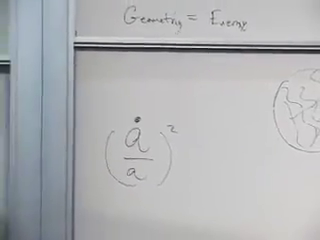
\includegraphics[width=0.68\textwidth]{lecture_06_figure_03.png}
\lectureframe{01:06:37.088}
\caption{Khẩu hiệu định hướng \emph{hình học bằng năng lượng}, với hạng giãn nở \(H^2=(\dot a/a)^2\) được viết bên dưới.}
\end{figure}

Đối với một vũ trụ đồng nhất và đẳng hướng, phương trình Friedmann thứ nhất là
\begin{equation}
H^2+\frac{k}{a^2}
=\frac{8\pi G}{3}\rho,
\end{equation}
trong đơn vị \(c=1\), trong đó \(k=+1,0,-1\) biểu thị hình học không gian đóng, phẳng hoặc mở và
\begin{equation}
\rho
=\rho_{\mathrm{ordinary}}
+\rho_{\mathrm{dark}}
+\rho_{\mathrm{radiation}}
+\rho_{\mathrm{vacuum}}.
\end{equation}
Dấu xuất hiện cạnh \(1/a^2\) phụ thuộc vào việc hạng độ cong được giữ ở vế trái hay chuyển sang vế phải, cũng như vào giá trị của \(k\).

\begin{figure}[H]
\centering
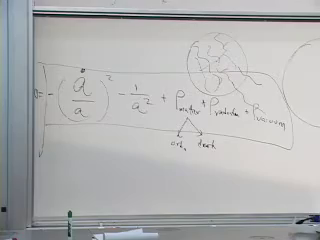
\includegraphics[width=0.96\textwidth]{lecture_06_figure_04.png}
\lectureframe{01:08:46.794}
\caption{Sự cân bằng đầy đủ trên bảng: giãn nở và độ cong không gian ở phía hình học, còn vật chất, bức xạ và năng lượng chân không ở phía nguồn. Vật chất còn được tách thêm thành các thành phần thường và tối.}
\end{figure}

\subsection{Ràng buộc Hamiltonian vũ trụ học}

\begin{classroomqa}
\audiencequestion{Nếu năng lượng chân không trong một vùng đồng chuyển động tăng lên khi vũ trụ giãn nở, thì có một mật độ năng lượng ròng không đổi hay một tổng năng lượng được bảo toàn không? \lecturetimestamp{01:01:51}}
\lecturerresponse{Thuyết tương đối rộng không cung cấp một năng lượng toàn cục phổ quát cho một không-thời gian giãn nở tùy ý. Tuy nhiên, trong phép rút gọn vũ trụ học đồng nhất, phương trình Einstein thành phần thời-thời là một ràng buộc Hamiltonian. Khi hình học và vật chất được đưa về cùng một vế, Hamiltonian chịu ràng buộc ấy bằng không. Các hạng vật chất đang biến đổi được cân bằng bởi các bậc tự do hấp dẫn, chứ không phải bởi một năng lượng cố định thông thường trong một cái hộp.}
\end{classroomqa}

Dưới dạng sơ đồ, phát biểu chính tắc là
\begin{equation}
\mathcal H_{\mathrm{gravity}}
+\mathcal H_{\mathrm{matter}}
=0.
\end{equation}
Đây là ý nghĩa chính xác của câu nói rằng tổng năng lượng bằng không. Đó là một phương trình chuyển động được áp đặt bởi tính bất biến đối với tái tham số hóa thời gian, chứ không phải là khẳng định rằng mọi mật độ năng lượng cục bộ đều triệt tiêu. Trong một thể tích đồng chuyển động, năng lượng của vật chất thông thường xấp xỉ cố định, năng lượng bức xạ giảm xuống, còn năng lượng chân không tăng lên; đồng thời, phần đóng góp hấp dẫn và tốc độ giãn nở tự điều chỉnh để ràng buộc của Einstein vẫn được thỏa mãn.

Bảo toàn cục bộ vẫn chính xác:
\begin{equation}
\nabla_\mu T^{\mu\nu}=0.
\end{equation}
Đối với chất lưu đồng nhất, đây chính là phương trình liên tục
\(\dot\rho+3H(\rho+p)=0\). Điều nói chung không còn đúng là trực giác từ không-thời gian phẳng cho rằng cũng phải tồn tại một tổng toàn cục của năng lượng vật chất, độc lập tọa độ, được bảo toàn trong một vũ trụ giãn nở.\editorialnote{Phân biệt này làm cho phát biểu trên lớp rằng năng lượng luôn bằng không trở nên chính xác: bảo toàn hiệp biến cục bộ và ràng buộc Hamiltonian vũ trụ học là chính xác, còn một năng lượng toàn cục duy nhất của vật chất cộng hấp dẫn thì nói chung không được định nghĩa.}

\begin{classroomqa}
\audiencequestion{Ràng buộc bằng không có phải là điều kiện quyết định vũ trụ là mở, đóng hay phẳng không? \lecturetimestamp{01:04:42}}
\lecturerresponse{Không. Ràng buộc Hamiltonian áp dụng trong mọi trường hợp. Các vũ trụ mở, phẳng và đóng khác nhau qua nhãn độ cong \(k\) và vì vậy qua hạng \(k/a^2\). Độ cong làm thay đổi một đóng góp trong sự cân bằng; nó không làm cho ràng buộc ấy có hiệu lực hay mất hiệu lực.}
\end{classroomqa}

\section{Tọa độ Grassmann và siêu trường}

\begin{classroomqa}
\audiencequestion{Các số Grassmann có thật sự xuất hiện trong Lagrangian của lý thuyết không? \lecturetimestamp{01:09:37}}
\lecturerresponse{Trước hết chúng xuất hiện vì các trường fermion là lẻ Grassmann. Chúng xuất hiện lần thứ hai như các tọa độ của siêu không gian. Các siêu trường phụ thuộc vào các tọa độ lẻ đó, và các tác dụng siêu đối xứng được xây dựng bằng cách lấy đạo hàm và tích phân theo chúng.}
\end{classroomqa}

Một trường thông thường là một hàm của không-thời gian,
\begin{equation}
\phi=\phi(x^\mu).
\end{equation}
Siêu đối xứng tối thiểu trong bốn chiều mở rộng \(x^\mu\) bằng một spinor lẻ hai thành phần \(\theta^\alpha\) và liên hợp của nó \(\bar\theta^{\dot\alpha}\):
\begin{equation}
z^M=(x^\mu,\theta^\alpha,\bar\theta^{\dot\alpha}).
\end{equation}
Có hai thành phần lẻ phức, hay bốn hướng lẻ thực. Một siêu trường là một hàm trên siêu không gian này:
\begin{equation}
\Phi=\Phi(x,\theta,\bar\theta).
\end{equation}

Đây không phải là những chiều không gian cực nhỏ theo nghĩa metric. Một tọa độ Grassmann không có độ lớn số học dương. Việc gọi nó là nhỏ chỉ là một cách gợi nhớ đến tính lũy linh:
\begin{equation}
(\theta^\alpha)^2=0,
\qquad
\theta^\alpha\theta^\beta=-\theta^\beta\theta^\alpha.
\end{equation}
\editorialnote{Chính tính lũy linh, chứ không phải sự nhỏ theo trị số, là lý do mọi khai triển theo một số hữu hạn tọa độ Grassmann đều kết thúc.}

Với bốn tọa độ lẻ độc lập, một siêu trường hoàn toàn tổng quát có nhiều nhất \(2^4=16\) đơn thức Grassmann. Dưới dạng sơ đồ,
\begin{equation}
\begin{aligned}
\Phi(x,\Theta)={}&\phi(x)+\Theta_A\psi_A(x)\\
&+\frac{1}{2}\Theta_A\Theta_B Z_{AB}(x)+\cdots\\
&+\Theta_1\Theta_2\Theta_3\Theta_4D(x),
\end{aligned}
\end{equation}
trong đó \(\Theta_A\) ký hiệu gộp cho bốn tọa độ lẻ thực. Vì toàn bộ siêu trường có thể được chọn là chẵn, nên các hệ số của những hạng bậc chẵn là bosonic còn các hệ số của những hạng bậc lẻ là fermionic. Vì thế, một siêu trường gói gọn một đa bội hữu hạn các trường thành phần thông thường.

Cách gói gọn này không chỉ là ký hiệu. Siêu đối xứng tác động về mặt hình học như một phép tịnh tiến theo các hướng lẻ đan xen với phép tịnh tiến trong không-thời gian. Một Lagrangian được xây dựng từ các siêu trường theo các quy tắc của siêu không gian sẽ thừa hưởng đối xứng đó theo cùng cách mà một Lagrangian vô hướng được xây dựng từ các tensor thừa hưởng tính bất biến quay hay Lorentz.

Tác dụng bây giờ bao gồm các độ đo Grassmann. Một hạng điển hình trên toàn siêu không gian có dạng
\begin{equation}
S_D=\int d^4x\,d^2\theta\,d^2\bar\theta\,
\mathcal K(\Phi,\Phi^\dagger).
\end{equation}
Còn các hạng chiral thì dùng
\begin{equation}
S_F=\int d^4x\,d^2\theta\,W(\Phi)+\mathrm{h.c.}
\end{equation}
\editorialnote{Sự phân biệt giữa độ đo trên toàn siêu không gian và độ đo chiral là sự tinh chỉnh tiêu chuẩn của tác dụng sơ đồ \(d^4x\,d^4\theta\). Các ví dụ cụ thể sẽ quyết định độ đo nào là thích hợp.}

Vì thế, ta đã đi tới một câu hỏi mà phép tính thông thường không trả lời được: tích phân trên một tọa độ phản giao hoán có nghĩa là gì?

\section{Tích phân Berezin}

\subsection{Mô hình thông thường: một đạo hàm toàn phần}

Hãy bắt đầu với một hàm thông thường \(F(x)\) triệt tiêu khi \(x\) dương rất lớn và âm rất lớn. Định lý cơ bản của giải tích cho
\begin{equation}
\int_{-\infty}^{\infty}dx\,\frac{dF}{dx}
=F(\infty)-F(-\infty)
=0.
\end{equation}

\begin{figure}[H]
\centering
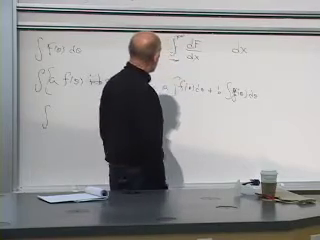
\includegraphics[width=0.88\textwidth]{lecture_06_figure_05.png}
\lectureframe{01:26:31.594}
\caption{Mẫu hình thông thường cho tích phân Berezin: tích phân của một đạo hàm toàn phần rút về các giá trị ở đầu mút và bằng không khi hàm tắt dần. Dòng phía dưới trên bảng bị che khuất một phần, nên phương trình rõ ràng được cung cấp trong phần văn bản.}
\end{figure}

Ta muốn tích phân Grassmann là tuyến tính và có chung tính chất hữu ích là tích phân của một đạo hàm toàn phần bằng không. Với một tọa độ lẻ, hãy yêu cầu
\begin{align}
\int d\theta\,[af(\theta)+bg(\theta)]
&=
a\int d\theta\,f(\theta)
+b\int d\theta\,g(\theta),\\
\int d\theta\,\partial_\theta f(\theta)&=0.
\end{align}
Điều kiện thứ hai là phép tương tự đại số của tính bất biến tịnh tiến của độ đo. Không có các đầu mút của một trục số lẻ, cũng không có tổng trên những khoảng cực nhỏ.

\begin{classroomqa}
\audiencequestion{Nếu không có tích phân Grassmann bất định, có phải ta đang từ bỏ ý tưởng rằng tích phân là phép nghịch đảo của đạo hàm không? \lecturetimestamp{01:21:19}}
\lecturerresponse{Vâng. Tích phân Berezin là một phiếm hàm tuyến tính xác định, không phải một phép lấy nguyên hàm. Với một biến Grassmann, trên thực tế nó được biểu diễn bởi cùng một phép toán đại số như phép đạo hàm.}
\end{classroomqa}

\begin{classroomqa}
\audiencequestion{Phép tích phân \(d^4x\) trên toàn bộ không-thời gian cũng là một tích phân xác định phải không? \lecturetimestamp{01:21:34}}
\lecturerresponse{Có. Khi người ta tích phân tác dụng trên không-thời gian, các điều kiện biên được hiểu ngầm. Khác biệt là tích phân thông thường trên không-thời gian có thể được hiểu qua giới hạn của các tổng, còn tích phân Grassmann được định nghĩa đại số bằng tác dụng của nó lên cơ sở hữu hạn \(1,\theta\).}
\end{classroomqa}

\subsection{Một biến}

Mọi hàm của một biến lẻ đều có thể được viết với hệ số ở bên phải theo thứ tự cố định
\begin{equation}
f(\theta)=a+\theta b.
\end{equation}
Vì \(\partial_\theta\theta=1\), quy tắc đạo hàm toàn phần suy ra
\begin{equation}
\int d\theta\,1=0.
\end{equation}
Chuẩn hóa còn lại được chọn là
\begin{equation}
\int d\theta\,\theta=1.
\end{equation}
Do đó,
\begin{equation}
\int d\theta\,f(\theta)=b.
\end{equation}
Tích phân chọn ra hệ số của lũy thừa cao nhất có thể có. Với quy ước đạo hàm trái dùng ở đây,
\begin{equation}
\partial_\theta f=b
=\int d\theta\,f.
\end{equation}

\begin{classroomqa}
\audiencequestion{Có tồn tại một hàm \(F(\theta)\) thỏa mãn \(\partial_\theta F=\theta\) không? \lecturetimestamp{01:30:05}}
\lecturerresponse{Không. Một hàm như vậy sẽ cần một hạng tỉ lệ với \(\theta^2\), nhưng \(\theta^2=0\). Đây là một cách khác để thấy vì sao không có tương tự Grassmann của một nguyên hàm bất định.}
\end{classroomqa}

\subsection{Hai biến và thứ tự của độ đo}

Đối với một cặp phức \(\theta,\bar\theta\), hãy viết một hàm chẵn tổng quát dưới dạng có thứ tự
\begin{equation}
f(\theta,\bar\theta)
=a+\bar\theta\psi+\bar\psi\theta+b\,\bar\theta\theta.
\end{equation}
Không có hạng bậc cao hơn nào vì
\begin{equation}
\theta^2=\bar\theta^2=0,
\qquad
\bar\theta\theta=-\theta\bar\theta.
\end{equation}

Bây giờ ta cố định quy ước
\begin{equation}
\int d\theta\,d\bar\theta\,
\bar\theta\theta=1.
\end{equation}
Với các tích phân lặp, phép toán \(d\bar\theta\) liền kề tác dụng trước. Khi đó bảng là
\begin{align}
\int d\theta\,d\bar\theta\,1&=0,\\
\int d\theta\,d\bar\theta\,\theta&=0,\\
\int d\theta\,d\bar\theta\,\bar\theta&=0,\\
\int d\theta\,d\bar\theta\,\bar\theta\theta&=1.
\end{align}
Do đó
\begin{equation}
\int d\theta\,d\bar\theta\,
f(\theta,\bar\theta)=b.
\end{equation}

\begin{classroomqa}
\audiencequestion{Đối với một hạng tuyến tính theo \(\theta\), có thật chính phép tích phân theo \(\theta\) làm cho tích phân kép triệt tiêu không? \lecturetimestamp{01:34:59}}
\lecturerresponse{Không; lời giải thích trực tiếp trên lớp đã đảo ngược vai trò của chúng. Tích phân \(\theta\) theo \(\theta\) cho ra 1. Khi đó kết quả không còn chứa \(\bar\theta\), và tích phân \(\bar\theta\) còn lại của 1 thì bằng không. Dù theo cách nào đi nữa, một tích phân kép chỉ còn lại khi cả hai biến đều hiện diện.}
\end{classroomqa}

\begin{classroomqa}
\audiencequestion{Nếu hoán đổi \(\theta\) và \(\bar\theta\), tích phân có đổi dấu không? \lecturetimestamp{01:36:33}}
\lecturerresponse{Có. Các biến lẻ và các độ đo lẻ phản giao hoán. Với quy ước ở trên,
\[
\int d\bar\theta\,d\theta\,\bar\theta\theta=-1.
\]
Vì thế, ta phải chọn một thứ tự và giữ nó nhất quán. Vật lý không phụ thuộc quy ước, nhưng các dấu trung gian thì có.}
\end{classroomqa}

Đối với \(n\) biến Grassmann độc lập, khuôn mẫu là hiển nhiên:
\begin{equation}
\int d\theta_n\cdots d\theta_1\,
f(\theta_1,\ldots,\theta_n)
\end{equation}
trích ra hệ số của đơn thức bậc cao nhất có thứ tự \(\theta_1\cdots\theta_n\), tới dấu được cố định bởi thứ tự đã chọn của các biến và các độ đo. Quy tắc trích xuất thành phần đơn giản này là động cơ đứng sau các tác dụng trên siêu không gian. Một biến thiên siêu đối xứng trở thành một đạo hàm toàn phần lẻ, và tích phân trên siêu không gian loại bỏ nó, cũng như một tác dụng thông thường loại bỏ một đạo hàm toàn phần theo không-thời gian dưới các điều kiện biên thích hợp.

\section{Vì sao một phép tính nhỏ như vậy lại có sức mạnh lớn đến thế}

Các quy tắc trông gần như tầm thường:
\begin{equation}
\int d\theta\,1=0,
\qquad
\int d\theta\,\theta=1.
\end{equation}
Thế nhưng chúng cho phép ta xây dựng các lý thuyết trường tương tác trong đó các quan hệ giữa các khối lượng bosonic và fermionic, cũng như giữa các hằng số ghép bosonic và fermionic, được duy trì tự động. Mục đích của phép tính trên siêu không gian cũng giống như mục đích của phép tính tensor trong thuyết tương đối: sắp xếp ký hiệu sao cho đối xứng mong muốn được duy trì qua mọi thao tác được phép.

Cái giá phải trả là việc theo dõi dấu. Mỗi lần hoán đổi hai đối tượng lẻ đều đóng góp một dấu trừ, và một phép tính có thể đúng về mặt ý niệm mà vẫn sai chỉ vì một lựa chọn thứ tự. Khó khăn đó không phải là thứ trang trí; nó là cái bóng đại số của thống kê fermion.

\begin{classroomqa}
\audiencequestion{Các số Grassmann được phát minh cùng với siêu đối xứng, hay chúng đã tồn tại từ trước? \lecturetimestamp{01:41:19}}
\lecturerresponse{Chúng lâu đời hơn rất nhiều. Hermann Grassmann đã phát triển đại số ngoại nền tảng ấy vào thế kỷ XIX. Các dạng vi phân vốn đã dùng các phần tử cơ sở phản giao hoán; lý thuyết trường lượng tử thế kỷ XX và siêu đối xứng đã tìm thấy một vai trò vật lý mới cho chính toán học đó.}
\end{classroomqa}

Giờ đây ta đã sẵn sàng cho những xây dựng cụ thể. Các siêu trường gom các đa bội boson-fermion đầy đủ, các đạo hàm trên siêu không gian bảo toàn đại số, và tích phân Berezin trích ra tác dụng thành phần. Nhiệm vụ tiếp theo là dùng bộ công cụ này trong mô hình một chiều đơn giản nhất rồi đưa nó vào lý thuyết trường.

\chapter{Siêu không gian và việc xây dựng động lực học siêu đối xứng}

\lectureoverview{Chúng ta xây dựng lại siêu đối xứng từ hệ nhỏ nhất mà nó có thể tác dụng lên: một dao động tử boson và một dao động tử fermion có cùng năng lượng. Sự tương phản giữa các phương trình bậc hai và bậc nhất của chúng dẫn đến các siêu điện tích và đại số của chúng. Sau đó ta diễn giải lại đại số ấy như hình học trên một không gian với tọa độ thông thường (t) và các tọa độ Grassmann \(\theta,\bar\theta\). Các siêu trường gộp boson, fermion và một trường phụ trợ vào một đối tượng duy nhất; phép tích phân Berezin rút ra một Lagrangian thông thường bất biến; các đạo hàm hiệp biến làm cho các ràng buộc tương thích với đối xứng trở nên khả dĩ; và ràng buộc chiral cung cấp ví dụ quan trọng đầu tiên. Bài giảng cố ý phơi bày các khó khăn về dấu và thứ tự của bộ máy này, rồi kết thúc bằng việc giải thích vì sao bản thân đối xứng còn cơ bản hơn một danh mục các quy tắc Feynman.}

\section{Trở lại hệ một mode}

Hãy bắt đầu lại với fermion và boson ở trạng thái nghỉ. Ta lược bỏ mọi tọa độ không gian và mọi nhãn động lượng. Trong một mode cho trước, một lượng tử có mặt hoặc vắng mặt, và các toán tử tạo, hủy là đủ để mô tả nó. Viết \(a^\dagger,a\) cho một mode boson và \(c^\dagger,c\) cho một mode fermion. Chúng thỏa mãn
\begin{align}
[a,a^\dagger]&=1,
&
\{c,c^\dagger\}&=1,
&
c^2=(c^\dagger)^2&=0.
\end{align}
Nếu hai lượng tử có cùng năng lượng \(m\), thì, ngoài một hằng số chân không không quan trọng,
\begin{equation}
H=m\left(a^\dagger a+c^\dagger c\right).
\label{eq:l7-one-mode-hamiltonian}
\end{equation}
Toán tử số \(a^\dagger a\) có thể nhận mọi giá trị nguyên không âm, còn \(c^\dagger c\) chỉ có thể bằng 0 hoặc 1. Đó là toàn bộ động học của mô hình đồ chơi này.

Sự đơn giản hóa này mang tính chiến lược. Ta muốn hiểu phép toán hủy một boson và tạo một fermion, hoặc làm điều ngược lại, mà không làm thay đổi năng lượng. Tuy nhiên, trước khi xây dựng phép toán đó, ta sẽ chuyển cùng hệ ấy từ ngôn ngữ toán tử sang ngôn ngữ Lagrangian.

\section{Dao động tử boson}

Đối với boson, đưa vào một tọa độ thực \(\phi(t)\). Khi không có biến thiên theo không gian, một trường vô hướng tự do trở thành một dao động tử điều hòa thông thường. Biểu thức đầu tiên được viết trên bảng là
\[
\frac{1}{2}\dot\phi^{,2}+\frac{1}{2}m^2\phi^2.
\]
Biểu thức đó là động năng cộng thế năng, không phải Lagrangian. Dấu được sửa ngay trong bài giảng:
\begin{equation}
L_B=\frac{1}{2}\dot\phi^{,2}-\frac{1}{2}m^2\phi^2.
\label{eq:l7-boson-lagrangian}
\end{equation}

\begin{figure}[H]
\centering
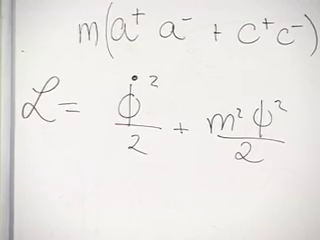
\includegraphics[width=0.62\textwidth]{lecture_07_figure_02.png}
\lectureframe{00:03:25.431}
\caption{Hamiltonian một mode ở phía trên Lagrangian boson. Khung hình giữ lại dấu cộng ban đầu trước khi được sửa bằng lời thành \(T-V\).}
\end{figure}

\begin{classroomqa}
\audiencequestion{Dấu trong Lagrangian dao động tử đang hiển thị sai ở chỗ nào? \lecturetimestamp{00:04:00}}
\lecturerresponse{Năng lượng là \(T+V\), còn Lagrangian là \(T-V\). Vì vậy số hạng thế phải mang dấu trừ. Sự hiệu chỉnh này biến phương trình từ hành vi mũ thành dao động điều hòa như dự định.}
\end{classroomqa}

Thật vậy, phương trình Euler--Lagrange cho
\begin{align}
\frac{d}{dt}\frac{\partial L_B}{\partial\dot\phi}
&=\frac{\partial L_B}{\partial\phi},\\
\ddot\phi&=-m^2\phi,
\end{align}
hoặc
\begin{equation}
\ddot\phi+m^2\phi=0.
\label{eq:l7-boson-eom}
\end{equation}
Tần số của nó là \(m\), không phải \(m^2\). Lượng tử hóa dao động tử này tạo ra cùng một thang trạng thái được mô tả bởi \(a^\dagger\) và \(a\) trong phương trình~\eqref{eq:l7-one-mode-hamiltonian}.

\section{Vì sao tác dụng của fermion là bậc nhất}

Lagrangian fermion trông đơn giản hơn vì nó chỉ chứa một đạo hàm theo thời gian. Lý do đã lộ ra ngay trong một phép thử cố ý ngây thơ. Với một biến giao hoán thông thường,
\begin{equation}
L_{\mathrm{trial}}=\phi\dot\phi
=\frac{1}{2}\frac{d}{dt}\phi^2.
\end{equation}
Đó là một đạo hàm toàn phần. Phương trình Euler--Lagrange của nó chỉ nói \(\dot\phi=\dot\phi\), nên mọi quỹ đạo khả vi đều được phép. Loại bỏ một đạo hàm toàn phần khỏi tác dụng làm thay đổi dữ liệu ở biên chứ không làm thay đổi phương trình chuyển động trong nội miền.

Bây giờ hãy đổi tên biến thành \(\psi\) và tuyên bố nó là lẻ Grassmann. Cả \(\psi\) lẫn \(\dot\psi\) đều phản giao hoán. Với lựa chọn cố định là biến phân bên trái, việc sắp xếp lại các thừa số lẻ đưa vào một dấu trừ, nên cùng phép thử hình thức đó cho
\begin{equation}
\frac{d}{dt}\frac{\partial L_{\mathrm{trial}}}{\partial\dot\psi}
=\dot\psi,
\qquad
\frac{\partial L_{\mathrm{trial}}}{\partial\psi}
=-\dot\psi.
\end{equation}
Vì vậy phương trình là
\begin{equation}
\dot\psi=-\dot\psi
\quad\Longrightarrow\quad
\dot\psi=0.
\label{eq:l7-constant-fermion}
\end{equation}
Biểu thức vốn là một hằng đẳng thức đối với một tọa độ giao hoán nay đã có nội dung động lực học đối với một tọa độ phản giao hoán. Nó có quá nhiều nội dung đối với một dao động tử, vì nó chỉ cho phép một hằng số, nhưng chính đó lại là đầu mối ta cần.

\begin{classroomqa}
\audiencequestion{Có phải nghiệm đơn giản chỉ là \(\psi\) là hằng số không? \lecturetimestamp{00:13:57}}
\lecturerresponse{Đúng. Phương trình~\eqref{eq:l7-constant-fermion} là một phương trình vi phân bậc nhất đích thực, và nghiệm của nó là một hằng tùy ý nhận giá trị Grassmann. Một số hạng khối lượng sẽ biến nghiệm tĩnh ấy thành một nghiệm dao động.}
\end{classroomqa}

Cố gắng hiển nhiên, \(m\psi^2\), thất bại vì \(\psi^2=0\). Ta cần hai biến lẻ thực \(\psi_1,\psi_2\), hoặc tương đương là một biến phức và liên hợp của nó. Bài giảng triển khai dạng hai biến thực trên bảng, liên tục kiểm tra các dấu và các hệ số 2. Một dạng phức được chuẩn hóa theo quy ước là
\begin{equation}
L_F=\frac{i}{2}
\left(\bar\psi\dot\psi-\dot{\bar\psi}\psi\right)
-m\bar\psi\psi.
\label{eq:l7-fermion-lagrangian}
\end{equation}
Sai khác bởi một đạo hàm toàn phần, biểu thức này là \(i\bar\psi\dot\psi-m\bar\psi\psi\). Biến phân theo \(\bar\psi\) cho
\begin{equation}
i\dot\psi=m\psi,
\qquad
\psi(t)=\psi(0)e^{-imt}.
\label{eq:l7-fermion-eom}
\end{equation}
Phương trình liên hợp có pha ngược lại. Vì thế mode fermion dao động với năng lượng \(m\), cũng như mode boson, mặc dù phương trình của nó là bậc nhất chứ không phải bậc hai.

\editorialnote{Phương trình~\eqref{eq:l7-fermion-lagrangian} cố định một quy ước chuẩn về thứ tự và chuẩn hóa cho phép tính thăm dò với hai biến thực. Chính bài giảng đưa vào thừa số \(i\), điều chỉnh một hệ số 2, và để ngỏ một dấu của một thành phần thực. Những thay đổi này không làm thay đổi kết luận trung tâm của nó: động học fermion là bậc nhất, khối lượng xuất hiện tuyến tính, và một fermion phức cho một song tuyến tính khác không.}

Đây là hình chiếu không chiều của một sự tương phản tương đối tính quen thuộc. Phương trình Klein--Gordon là bậc hai theo thời gian, còn phương trình Dirac là bậc nhất. Khi đã lược bỏ không gian, boson là một dao động tử điều hòa và fermion là một dao động tử Grassmann phức.

\begin{classroomqa}
\audiencequestion{Thứ tự viết \(\psi\), \(\dot\psi\) và các liên hợp của chúng có quan trọng không? \lecturetimestamp{00:18:58}}
\lecturerresponse{Các công thức trung gian quả thật phụ thuộc vào thứ tự vì các thừa số lẻ phản giao hoán. Lý thuyết vật lý thì không phụ thuộc vào một sở thích ghi chép tùy tiện, miễn là từ đầu đến cuối người ta dùng một quy ước duy nhất cho biến phân trái hay phải, phép liên hợp và phép tích phân. Đảo thứ tự một cặp lẻ làm đổi một dấu, và dấu ấy phải được đổi một cách nhất quán ở mọi chỗ khác.}
\end{classroomqa}

Kết hợp các phương trình~\eqref{eq:l7-boson-lagrangian} và \eqref{eq:l7-fermion-lagrangian} cho một mô tả Lagrangian của cùng một cặp tương ứng đã được biểu diễn bởi phương trình~\eqref{eq:l7-one-mode-hamiltonian}. Giờ đây ta đã sẵn sàng nhận diện đối xứng giữa chúng.

\section{Siêu điện tích và đại số của chúng}

Một toán tử hủy một fermion và tạo một boson là
\begin{equation}
Q^\dagger=\sqrt{2m}\,a^\dagger c,
\end{equation}
trong khi liên hợp của nó hủy một boson và tạo một fermion,
\begin{equation}
Q=\sqrt{2m}\,a c^\dagger.
\end{equation}
Sự chuẩn hóa được chọn sao cho đại số có dạng chuẩn. Dùng \(cc^\dagger=1-c^\dagger c\), \(aa^\dagger=a^\dagger a+1\), và thực tế rằng các toán tử boson và fermion giao hoán với nhau,
\begin{align}
\{Q,Q^\dagger\}
&=2m\left(ac^\dagger a^\dagger c+a^\dagger c a c^\dagger\right)\notag\\
&=2m\left[(a^\dagger a+1)c^\dagger c
+a^\dagger a(1-c^\dagger c)\right]\notag\\
&=2m\left(a^\dagger a+c^\dagger c\right)=2H.
\label{eq:l7-superalgebra}
\end{align}
Các toán tử boson có thể được chuyển qua các toán tử fermion. Chính tính lũy linh vốn giới hạn số chiếm chỗ fermion cho
\begin{equation}
Q^2=(Q^\dagger)^2=0.
\end{equation}
Cuối cùng,
\begin{equation}
[H,Q]=[H,Q^\dagger]=0.
\label{eq:l7-conserved-supercharges}
\end{equation}
Mỗi siêu điện tích làm thay đổi số boson và số fermion theo hai chiều ngược nhau, nên hai độ thay đổi năng lượng triệt tiêu nhau khi các tần số bằng nhau.

\begin{classroomqa}
\audiencequestion{\([H,Q]\) là gì? Có phải đáp án tỉ lệ với \(Q\) không? \lecturetimestamp{00:25:10}}
\lecturerresponse{Không. Đáp án bằng 0. Một toán tử tạo hoặc hủy đơn lẻ sẽ nhận năng lượng của nó khi lấy giao hoán với \(H\), nhưng các đóng góp boson và fermion trong \(Q\) triệt tiêu nhau. Sự triệt tiêu ấy chính là điều kiện cùng năng lượng.}
\end{classroomqa}

\begin{classroomqa}
\audiencequestion{Giao hoán tử ấy chẳng phải đã được viết trên bảng rồi sao? \lecturetimestamp{00:25:45}}
\lecturerresponse{Đúng vậy. Việc tìm lại nó vẫn hữu ích vì nó buộc ta phải diễn giải chứ không chỉ chép lại hệ thức: giao hoán với Hamiltonian có nghĩa là phép biến đổi ấy là một đối xứng và bộ sinh của nó được bảo toàn.}
\end{classroomqa}

Tính từ \emph{điện tích} phản ánh định luật bảo toàn này. Tuy nhiên, ta không nên coi \(Q\) như một con số thông thường có thể đo đồng thời gắn với một trạng thái. Nó là lẻ Grassmann, lũy linh, và ánh xạ một trạng thái boson thành một trạng thái fermion. Phát biểu hữu ích là nó là một bộ sinh được bảo toàn, tác động trong các siêu đa bội suy biến.
\editorialnote{Cách diễn đạt này chỉnh lý phép so sánh trên lớp học giữa việc gắn nhãn các trạng thái bằng năng lượng hay điện tích điện. Các siêu điện tích lẻ riêng lẻ, không Hermite, không phải là những quan sát lượng thông thường với các nhãn lượng tử bằng số. Tác động được bảo toàn của chúng và biểu diễn của toàn bộ siêu đại số mới đem lại sự phân loại đúng.}

\section{Các bộ sinh dưới dạng đạo hàm}

Đại số thì súc tích, nhưng tự nó không cho ta biết phải xây dựng các lý thuyết có tương tác như thế nào. Bước tiếp theo mang tính hình học. Những bộ sinh đối xứng quen thuộc vốn đã tác dụng như các toán tử vi phân. Theo quy ước của bài giảng,
\begin{equation}
H=i\frac{\partial}{\partial t},
\qquad
P=-i\frac{\partial}{\partial x}.
\end{equation}

\begin{figure}[H]
\centering
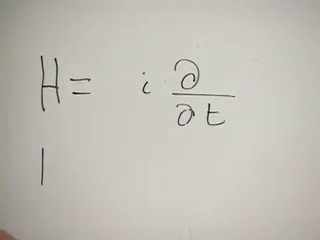
\includegraphics[width=0.50\textwidth]{lecture_07_figure_03.png}
\lectureframe{00:28:12.720}
\caption{Hamiltonian được biểu diễn như bộ sinh của các phép tịnh tiến theo thời gian.}
\end{figure}

Mômen góc cũng tương tự: một tọa độ nhân với một đạo hàm. Nếu các siêu điện tích là các bộ sinh lẻ, thì tự nhiên ta sẽ hỏi liệu chúng có thể được biểu diễn bằng các đạo hàm theo các tọa độ lẻ hay không. Vì vậy ta mở rộng trục thời gian thành siêu không gian
\begin{equation}
(t,\theta,\bar\theta),
\qquad
\theta^2=\bar\theta^2=0,
\qquad
\theta\bar\theta=-\bar\theta\theta.
\end{equation}
Các trường trên không gian này phụ thuộc vào một thời gian thông thường và một cặp tọa độ Grassmann liên hợp.

Bài giảng cố ý cho thấy các dấu dễ gây nhầm lẫn đến mức nào. Dấu do liên hợp phức, dấu do chuyển một tham số lẻ, và dấu do chọn đạo hàm trái thay cho đạo hàm phải tương ứng với những thao tác khác nhau. Thay vì giữ lại các bước trình bày trên bảng vốn không tương thích lẫn nhau, giờ đây ta cố định một quy ước: mọi đạo hàm lẻ đều là đạo hàm trái, và
\begin{equation}
q=\partial_\theta+i\bar\theta\partial_t,
\qquad
\bar q=\partial_{\bar\theta}+i\theta\partial_t.
\label{eq:l7-differential-supercharges}
\end{equation}
Khi đó
\begin{equation}
q^2=\bar q^{,2}=0,
\qquad
\{q,\bar q\}=2i\partial_t=2H.
\label{eq:l7-differential-algebra}
\end{equation}
Hệ số 2 xuất phát từ hai hạng chéo: \(\{\partial_\theta,\theta\}=1\) và \(\{\partial_{\bar\theta},\bar\theta\}=1\). Nếu các toán tử sinh chỉ chứa \(\partial_\theta\) và \(\partial_{\bar\theta}\), thì phản giao hoán tử của chúng sẽ triệt tiêu và không thể tái tạo Hamiltonian.

\begin{classroomqa}
\audiencequestion{Hai số hạng đạo hàm theo thời gian trong \(q\) và \(\bar q\) có phải mang cùng dấu không? \lecturetimestamp{00:31:01}}
\lecturerresponse{Chúng phải được chọn nhất quán sao cho phản giao hoán tử hỗn hợp là \(2H\). Có thể dùng hoặc một quy ước dấu cộng tổng thể, hoặc phương án liên hợp nhất quán của nó. Chính phép tính, chứ không phải trực giác hình ảnh về ký hiệu \(i\), mới quyết định các dấu tương đối.}
\end{classroomqa}

Cả phòng liên tục kiểm tra các dấu, và sự khó khăn trở thành một trò đùa: các dấu dường như thay đổi trên đường đi làm. Trò đùa ấy rất đúng chỗ. Việc phản giao hoán một tham số Grassmann qua một tọa độ có thể làm đổi dấu ngay cả khi không có quy ước vật lý nào thay đổi. Phương trình~\eqref{eq:l7-differential-supercharges} là mốc tham chiếu cố định cho mọi điều tiếp theo.

\subsection{Siêu đối xứng như một phép dịch tọa độ}

Cho \(\xi,\bar\xi\) là các tham số lẻ vô cùng bé. Tác dụng lên một siêu trường bằng
\begin{equation}
\delta_\xi=\xi q+\bar\xi\bar q
\end{equation}
tương đương, theo quy ước ở trên, với phép biến đổi tọa độ vô cùng bé
\begin{align}
\theta&\longrightarrow\theta+\xi,\\
\bar\theta&\longrightarrow\bar\theta+\bar\xi,\\
t&\longrightarrow t+i\left(\xi\bar\theta+\bar\xi\theta\right).
\label{eq:l7-coordinate-shift}
\end{align}
Vì vậy độ biến thiên của một siêu trường vô hướng là
\begin{equation}
\delta_\xi\Phi
=\left(\xi\partial_\theta+\bar\xi\partial_{\bar\theta}
+i\xi\bar\theta\partial_t+i\bar\xi\theta\partial_t\right)\Phi
=\left(\xi q+\bar\xi\bar q\right)\Phi.
\end{equation}
Đây là nội dung hình học của siêu đối xứng. Nó là một phép tịnh tiến theo các hướng lẻ gắn với một phép tịnh tiến theo thời gian thông thường. Hai phép dịch lẻ khép lại thành một phép tịnh tiến theo thời gian do phương trình~\eqref{eq:l7-differential-algebra}.

\begin{classroomqa}
\audiencequestion{Dấu trừ đang bị tranh luận đó có thể biểu diễn một chuyển động lùi về thời gian không? \lecturetimestamp{00:58:13}}
\lecturerresponse{Một quy ước dấu khác có thể đảo chiều phép dịch thời gian vô cùng bé được hiển thị, nhưng không có quá trình vật lý lùi-thời gian riêng biệt nào được đưa vào. Điều quan trọng là phép biến đổi tọa độ và các bộ sinh vi phân tuân theo cùng một đại số.}
\end{classroomqa}

\begin{classroomqa}
\audiencequestion{Thời gian mở rộng này có sự hiện thực hóa vật lý hay chỉ là một công cụ hạch toán hình thức? \lecturetimestamp{00:58:23}}
\lecturerresponse{Theo một nghĩa hữu ích thì đúng là một công cụ hạch toán: nó đóng gói đại số vào hình học. Nhưng sự đóng gói ấy trở nên có giá trị vật lý khi đưa các tương tác vào. Siêu không gian cung cấp một phép tính có hệ thống để xây dựng các Lagrangian bảo toàn đối xứng boson--fermion ở mọi bước, cũng như phép tính tensor giúp ta xây dựng các vô hướng Lorentz.}
\end{classroomqa}

\section{Siêu trường và thành phần phụ trợ}

Vì chỉ có hai tọa độ lẻ, khai triển của một siêu trường chẵn sẽ dừng lại:
\begin{equation}
\Phi(t,\theta,\bar\theta)
=\phi(t)+\bar\theta\psi(t)+\bar\psi(t)\theta
+D(t)\bar\theta\theta.
\label{eq:l7-superfield}
\end{equation}
Hệ số của các đơn thức chẵn, \(\phi\) và \(D\), mang tính boson; hệ số của các đơn thức lẻ, \(\psi\) và \(\bar\psi\), mang tính fermion. Không có hạng \(\theta^2\), \(\bar\theta^2\) hay bậc cao hơn nào còn tồn tại. Ta để phụ thuộc thời gian ở dạng chưa khai triển vì một chuỗi Taylor thông thường theo \(t\) sẽ không dừng lại và ở đây không phục vụ mục đích nào.

\begin{classroomqa}
\audiencequestion{Thành phần \(D(t)\) ở hạng trên cùng là gì? \lecturetimestamp{00:41:46}}
\lecturerresponse{Ở giai đoạn này, nó đơn giản chỉ là hệ số bosonic cuối cùng trong khai triển hữu hạn. Trong tác dụng theo thành phần, nó thông thường không có hạng động năng và bị khử bằng một phương trình chuyển động đại số, nên được gọi là một trường phụ trợ. Bài giảng đùa rằng ``D là viết tắt của dummy,'' điều này nêu bật vai trò không động lực học của nó dù đó không phải là định nghĩa lịch sử.}
\end{classroomqa}

Siêu trường là một đối tượng duy nhất, còn \(\phi,\psi,\bar\psi,D\) là các thành phần của nó. Một phép biến đổi siêu đối xứng trộn lẫn chúng. Vì thế một boson và một fermion có quan hệ với nhau theo gần như cùng nghĩa cấu trúc mà các thành phần \(x\)- và \(y\)- của một vectơ có quan hệ với nhau dưới một phép quay, mặc dù không thể hình dung các phương Grassmann như các trục thông thường.

\section{Siêu tác dụng và thành phần trên cùng}

Để thu được các phương trình chuyển động, ta cần một tác dụng. Trong lý thuyết trường thông thường, người ta lập một Lagrangian vô hướng và tích phân nó trên không-thời gian. Ở đây biểu thức tương tự là
\begin{equation}
S=\int dt\,d\theta\,d\bar\theta\;\Lambda
\bigl(\Phi,\text{ superspace derivatives of }\Phi\bigr),
\label{eq:l7-superaction}
\end{equation}
trong đó \(\Lambda\) là một siêu trường chẵn. Tích phân Berezin là đại số. Ta chọn
\begin{equation}
\int d\theta\,d\bar\theta\;\bar\theta\theta=1.
\end{equation}
Vì vậy, nếu
\begin{equation}
\Lambda=A+\bar\theta B+\bar B\theta+C\bar\theta\theta,
\end{equation}
thì
\begin{equation}
\int d\theta\,d\bar\theta\;\Lambda=C.
\label{eq:l7-top-component}
\end{equation}
Tích phân theo các biến lẻ rút ra thành phần trên cùng, để lại một Lagrangian thông thường sẽ được tích phân theo thời gian.

Vì sao kết quả là bất biến? Một biến phân siêu đối xứng tịnh tiến các biến tích phân. Biến phân của thành phần trên cùng là một đạo hàm toàn phần thông thường theo thời gian, còn các đạo hàm toàn phần theo biến lẻ triệt tiêu dưới tích phân Berezin. Với các điều kiện đầu mút thích hợp, tác dụng không đổi. Đây là phép tương tự trong siêu không gian của việc xây dựng một vô hướng Lorentz trước khi tích phân nó trên không-thời gian.

\section{Nhân các siêu trường}

Cách đơn giản nhất để tạo một siêu trường mới từ một siêu trường cũ là nhân nó với chính nó. Bắt đầu từ phương trình~\eqref{eq:l7-superfield}, mọi hạng chứa \(\theta^2\) hoặc \(\bar\theta^2\) đều triệt tiêu. Giữ thứ tự \(\bar\theta\theta\) và viết các trường thành phần có gạch trên ở bên trái, ta được
\begin{align}
\Phi^2
={}&\phi^2
+2\phi\bar\theta\psi
+2\phi\bar\psi\theta\notag\\
&+\left(2\phi D-2\bar\psi\psi\right)\bar\theta\theta.
\label{eq:l7-superfield-square}
\end{align}

\begin{figure}[H]
\centering
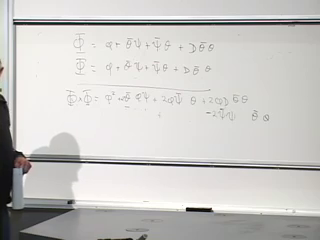
\includegraphics[width=0.82\textwidth]{lecture_07_figure_05.png}
\lectureframe{01:07:57.844}
\caption{Tích siêu trường theo từng thành phần và việc thu gom các hạng \(\bar\theta\theta\) của nó.}
\end{figure}

Hai hạng \(\phi D\) và \(D\phi\) cộng lại vì cả hai trường đều chẵn. Hai hạng chéo fermion cũng cộng lại sau khi mỗi hạng được sắp xếp lại, nhưng dấu chung của chúng là âm:
\begin{equation}
(\bar\theta\psi)(\bar\psi\theta)
+(\bar\psi\theta)(\bar\theta\psi)
=-2\bar\psi\psi\,\bar\theta\theta.
\end{equation}
Tích phân bình phương ấy theo các tọa độ lẻ cho
\begin{equation}
\int d\theta\,d\bar\theta\;\Phi^2
=2\phi D-2\bar\psi\psi.
\end{equation}
Hạng này là siêu đối xứng do được xây dựng như vậy, nhưng nó vẫn chưa phải là một Lagrangian động năng. Nó không chứa đạo hàm theo thời gian.

Sau đó trên bảng đề xuất \(\Phi^3\), \(\Phi^4\) và \(\Phi^n\) làm bài tập. Có một quy tắc gọn. Với mọi hàm thường \(W\),
\begin{equation}
\left.W(\Phi)\right|_{\bar\theta\theta}
=W'(\phi)D-W''(\phi)\bar\psi\psi.
\label{eq:l7-function-top-component}
\end{equation}
Với \(W(\phi)=\phi^2\), ta khôi phục lại phương trình~\eqref{eq:l7-superfield-square}; với \(W(\phi)=\phi^n\), ta được
\begin{equation}
\left.\Phi^n\right|_{\bar\theta\theta}
=n\phi^{n-1}D-n(n-1)\phi^{n-2}\bar\psi\psi.
\end{equation}
\editorialnote{Bài giảng giao lũy thừa bậc \(n\) làm bài tập và nêu các loại hạng tử được mong đợi. Phương trình~\eqref{eq:l7-function-top-component} cho quy tắc hoàn chỉnh trong quy ước thứ tự cố định.}

Tới đây giảng viên hỏi liệu cả phòng có kiệt sức chưa. Khán giả đáp là chưa; ông trả lời rằng người kiệt sức là ông. Trao đổi ấy không chỉ để gây cười. Lũy thừa của siêu trường thì dễ vì khai triển dừng lại, nhưng đạo hàm và ràng buộc mới là chỗ việc theo dõi dấu trở nên thực sự đòi hỏi.

\section{Những đạo hàm nào tương thích với siêu đối xứng?}

Có một chỗ cần sửa trước khi theo dõi lập luận tiếp theo trên bảng. Đạo hàm thời gian thông thường là vô hại:
\begin{equation}
[\partial_t,q]=[\partial_t,\bar q]=0.
\end{equation}
Do đó \(\partial_t\Phi\) biến đổi như một siêu trường mỗi khi \(\Phi\) biến đổi như vậy. Những đối tượng tinh tế là các đạo hàm lẻ trần \(\partial_\theta\Phi\) và \(\partial_{\bar\theta}\Phi\), vì chúng không phản giao hoán với cả hai siêu điện tích. Ta cần các đạo hàm lẻ đã hiệu chỉnh cho các ràng buộc và cho các phép xây dựng theo thành phần hiển nhiên siêu đối xứng.
\editorialnote{Phát biểu bằng lời rằng phép vi phân theo thời gian không cho ra một siêu trường khác là không đúng trong quy ước được dùng ở đây. Vì \(\partial_t\) giao hoán với cả hai siêu điện tích nên nó là hiệp biến. Việc xây dựng tiếp theo các đạo hàm lẻ đã hiệu chỉnh vẫn là cần thiết và mới là điểm toán học thực sự của bài giảng.}

\subsection{Phép tương tự ``trường ma thuật''}

Bài giảng nêu động cơ cho tiêu chuẩn này bằng các phép quay thông thường. Cho \(f(x,y)\) thỏa mãn
\begin{equation}
\partial_y f=0.
\label{eq:l7-magic-constraint}
\end{equation}
Hãy gọi một hàm như vậy là ``trường ma thuật.'' Nó phụ thuộc vào \(x\) nhưng không phụ thuộc vào \(y\). Lớp các trường ma thuật có được bảo toàn dưới phép quay không? Với
\begin{equation}
L_z=-i\left(x\partial_y-y\partial_x\right),
\end{equation}
ta tìm được
\begin{equation}
[\partial_y,L_z]=i\partial_x\neq0.
\end{equation}
Vì vậy \(L_z f\) nói chung sẽ nhận thêm phụ thuộc vào \(y\) ngay cả khi ban đầu \(f\) thỏa phương trình~\eqref{eq:l7-magic-constraint}. Ràng buộc ấy không bất biến quay.

Bài học tổng quát thì đơn giản. Nếu một trường thỏa \(C\Phi=0\) và một đối xứng được sinh bởi \(G\), thì trường đã biến đổi vẫn còn bị ràng buộc khi giao hoán tử phân bậc của \(C\) và \(G\) triệt tiêu. Đối với hai toán tử lẻ, giao hoán tử phân bậc là một phản giao hoán tử.

\begin{classroomqa}
\audiencequestion{Khi nào một ràng buộc đặt lên một trường là tương thích với một đối xứng? \lecturetimestamp{01:17:56}}
\lecturerresponse{Khi toán tử ràng buộc giao hoán phân bậc với các bộ sinh đối xứng. Khi đó \(C(G\Phi)\) có thể được đưa qua \(G\) và rút về \(G(C\Phi)=0\). Ví dụ về phép quay thất bại vì \(\partial_y\) không giao hoán với bộ sinh quay.}
\end{classroomqa}

\subsection{Các đạo hàm lẻ hiệp biến}

Với các siêu điện tích được cố định bởi phương trình~\eqref{eq:l7-differential-supercharges}, hãy định nghĩa
\begin{equation}
\mathcal D=\partial_\theta-i\bar\theta\partial_t,
\qquad
\bar{\mathcal D}=\partial_{\bar\theta}-i\theta\partial_t.
\label{eq:l7-covariant-derivatives}
\end{equation}
Thay đổi duy nhất là dấu của hạng đạo hàm theo thời gian. Tính trực tiếp cho
\begin{align}
\{\mathcal D,q\}
&=\{\mathcal D,\bar q\}
=\{\bar{\mathcal D},q\}
=\{\bar{\mathcal D},\bar q\}=0,\\
\{\mathcal D,\bar{\mathcal D}\}&=-2i\partial_t.
\label{eq:l7-covariant-algebra}
\end{align}
Hai hạng chéo có thể khác không triệt tiêu lẫn nhau. Đây là phép tương tự lẻ của một đạo hàm hiệp biến: nó lấy đạo hàm mà vẫn bảo toàn luật biến đổi.

Bài giảng dùng \(D\) vừa cho thành phần phụ trợ vừa cho đạo hàm này. Ta dành \(D(t)\) cho thành phần và dùng dạng thư pháp \(\mathcal D\) cho toán tử.

\section{Ràng buộc chiral}

Giờ đây ta có thể áp đặt một ràng buộc không tầm thường vẫn được bảo toàn bởi siêu đối xứng:
\begin{equation}
\bar{\mathcal D}\Phi=0.
\label{eq:l7-chiral-constraint}
\end{equation}
Một trường như vậy được gọi là chiral. Nếu nó là chiral trước một phép biến đổi siêu đối xứng, thì
\begin{equation}
\bar{\mathcal D}(q\Phi)
=-q(\bar{\mathcal D}\Phi)=0,
\qquad
\bar{\mathcal D}(\bar q\Phi)
=-\bar q(\bar{\mathcal D}\Phi)=0.
\end{equation}
Vì thế toàn bộ siêu trường đã biến đổi vẫn nằm trong lớp bị ràng buộc ấy. Khác với điều kiện trường ma thuật, tính chiral là tương thích với đối xứng.

Để giải ràng buộc, hãy định nghĩa một tọa độ thời gian dịch chuyển
\begin{equation}
\tau=t+i\bar\theta\theta.
\label{eq:l7-chiral-time}
\end{equation}
Vì ta dùng đạo hàm trái,
\begin{equation}
\partial_{\bar\theta}\tau=i\theta,
\end{equation}
và do đó
\begin{equation}
\bar{\mathcal D}F(\tau,\theta)
=\left(\partial_{\bar\theta}-i\theta\partial_t\right)F(\tau,\theta)
=i\theta\partial_\tau F-i\theta\partial_\tau F=0.
\end{equation}
Vì vậy siêu trường chiral cục bộ tổng quát chỉ phụ thuộc vào \(\bar\theta\) thông qua \(\tau\):
\begin{equation}
\Phi_{\mathrm{ch}}(\tau,\theta)
=\phi(\tau)+\bar\psi(\tau)\theta.
\label{eq:l7-chiral-field-tau}
\end{equation}

\begin{classroomqa}
\audiencequestion{Sự phụ thuộc vào \(\tau\) và \(\theta\) có phải là dạng duy nhất thỏa ràng buộc chiral không? \lecturetimestamp{01:32:35}}
\lecturerresponse{Xét cục bộ thì có. Phương trình vi phân \(\bar{\mathcal D}\Phi=0\) nói chính xác rằng sự phụ thuộc độc lập vào \(\bar\theta\) có thể được hấp thụ vào tọa độ dịch chuyển \(\tau=t+i\bar\theta\theta\). Khai triển hữu hạn còn lại là một hàm của \(\tau\) cộng với một hạng tỉ lệ với \(\theta\).}
\end{classroomqa}

Khai triển lại theo tọa độ thời gian ban đầu,
\begin{align}
\phi(\tau)
&=\phi(t)+i\bar\theta\theta\dot\phi(t),\\
\bar\psi(\tau)\theta
&=\bar\psi(t)\theta,
\end{align}
vì hiệu chỉnh ở dòng thứ hai chứa \(\theta^2\). Do đó
\begin{equation}
\Phi_{\mathrm{ch}}(t,\theta,\bar\theta)
=\phi(t)+\bar\psi(t)\theta
+i\bar\theta\theta\dot\phi(t).
\label{eq:l7-chiral-field-components}
\end{equation}

\begin{classroomqa}
\audiencequestion{Khai triển Taylor của \(\phi(t+i\bar\theta\theta)\) có nên chứa một hạng bậc hai không? \lecturetimestamp{01:33:51}}
\lecturerresponse{Không. Hiệu chỉnh đầu tiên là \(i\bar\theta\theta\dot\phi\), và mọi hiệu chỉnh bậc cao hơn đều chứa \((\bar\theta\theta)^2=0\). Khán giả nhận ra điều này ngay lập tức; tính lũy linh đã cung cấp hai hạng đầu và chấm dứt chuỗi.}
\end{classroomqa}

Đó là sự gọn nhẹ của tính chiral. Siêu trường không bị ràng buộc trong phương trình~\eqref{eq:l7-superfield} có hai vị trí thành phần bosonic và hai vị trí thành phần fermionic. Điều kiện chiral loại bỏ vị trí phụ trợ độc lập trong ví dụ một chiều tối thiểu này và gắn thành phần trên cùng với \(\dot\phi\).

\section{Phép tính dừng lại đúng lúc}

Bước tiếp theo tự nhiên là kết hợp trường chiral với trường liên hợp của nó và lấy tích phân trên siêu không gian. Việc khai triển liên hợp được bắt đầu, và một người nghe hỏi liệu thứ tự \(\theta\bar\theta\) có phải đảo ngược dưới phép liên hợp hay không. Đến lúc ấy các dấu không còn có vẻ đáng tin nữa. Thay vì đoán bừa, phép tính dừng lại.

\begin{classroomqa}
\audiencequestion{Liệu ta có thể nghe kết luận chính ngay cả khi phép nhân với trường liên hợp được để lại sau không? \lecturetimestamp{01:37:30}}
\lecturerresponse{Có. Nếu các dấu và các phép liên hợp được xử lý nhất quán, một biểu thức trong siêu không gian xây từ một trường chiral và trường liên hợp của nó sẽ cho ra các hạng động năng bosonic và fermionic thông thường như mong muốn. Kết quả quan trọng đối với bài giảng này là nguyên lý xây dựng, chứ không phải một dòng cuối thiếu tin cậy được chép ra từ một phép tính khi đã mệt.}
\end{classroomqa}

Điểm dừng ấy nên được giữ rõ. Hình thức luận này không khoan nhượng: chỉ cần đặt sai một thừa số lẻ là đổi dấu, và cùng một quy ước phải được duy trì qua phép liên hợp, phép vi phân, phép nhân và phép tích phân. Phản ứng đúng khi làm mất mạch đó là sửa lại nó trước khi đi tiếp. Trong một quy ước chuẩn, tác dụng động năng quen thuộc được xây từ một tích liên hợp, nhưng phép rút gọn chi tiết theo thành phần của nó thuộc về phép tính sạch sẽ kế tiếp, chứ không phải việc phục dựng một dòng dang dở trên bảng.

\section{Vì sao đối xứng mới là điểm mấu chốt}

Một Lagrangian siêu đối xứng không chỉ đặt một boson và một fermion cạnh nhau. Nó ràng buộc khối lượng và tương tác của chúng sao cho chúng tạo thành một biểu diễn của siêu đại số. Trong một chân không siêu đối xứng chính xác, các thành viên của một siêu bội có khối lượng bằng nhau. Các đóng góp vòng của chúng có tương quan, và các hiệu ứng tử ngoại bosonic và fermionic triệt tiêu đúng trong những tổ hợp mà đối xứng áp đặt.

Đó là lý do bộ máy xây dựng này quan trọng. Ta có thể liệt kê các đỉnh Feynman và kiểm tra sự triệt tiêu sơ đồ này qua sơ đồ khác, nhưng khi ấy các sự triệt tiêu sẽ có vẻ ngẫu nhiên. Siêu đối xứng giải thích chúng theo đúng cách mà đối xứng Lorentz giải thích vì sao các biên độ tán xạ biến đổi nhất quán trong mọi hệ quy chiếu quán tính.

\editorialnote{Siêu đối xứng chính xác không hàm ý rằng mọi hiệu chỉnh tự năng lượng riêng lẻ đều triệt tiêu. Nó liên hệ các sự tái chuẩn hóa và loại bỏ những độ nhạy tử ngoại nhất định; các mệnh đề không tái chuẩn hóa phụ thuộc vào đại lượng xét đến, số chiều và số lượng siêu đối xứng. Phát biểu khái quát của bài giảng về sự triệt tiêu được giữ lại dưới dạng có điều kiện này.}

\begin{classroomqa}
\audiencequestion{Từ ``chiral'' được đánh vần thế nào? \lecturetimestamp{01:39:48}}
\lecturerresponse{C-H-I-R-A-L. Từ này dùng để chỉ ràng buộc \(\bar{\mathcal D}\Phi=0\); nó không phải là tính thuận tay hình học thông thường của một vật trong không gian ba chiều, mặc dù thuật ngữ này bắt nguồn từ cấu trúc tay trái và tay phải của các spinor tương đối tính.}
\end{classroomqa}

\begin{classroomqa}
\audiencequestion{Liệu có thể bỏ qua Lagrangian và đi thẳng tới các quy tắc Feynman siêu đối xứng không? \lecturetimestamp{01:40:00}}
\lecturerresponse{Dĩ nhiên ta có thể phát biểu các quy tắc đó, nhưng khi ấy các quan hệ giữa những hằng số ghép và các sự triệt tiêu do chúng tạo ra sẽ trông như những sự trùng hợp không có lời giải thích. Nội dung sâu hơn là đối xứng không-thời gian được tổng quát hóa. Lagrangian, hoặc một hình thức bất biến tương đương, làm lộ rõ nguyên nhân đó và sinh ra các quy tắc một cách có hệ thống.}
\end{classroomqa}

Giả sử mọi bậc của lý thuyết nhiễu loạn đều tình cờ cho ra các biên độ bất biến Lorentz mặc dù chưa hề nhắc đến các phép biến đổi Lorentz nào. Sau đủ nhiều phép tính, ta sẽ đòi hỏi một lời giải thích. Câu trả lời sẽ là đối xứng không-thời gian tổ chức mọi bậc ấy cùng một lúc. Vai trò của siêu không gian là tương tự: các dịch chuyển theo \(\theta,\bar\theta\) trộn các thành phần boson và fermion, và đại số của chúng khép kín thành các phép tịnh tiến trong không-thời gian.

\begin{classroomqa}
\audiencequestion{Có nên khai triển cả các tọa độ không gian thông thường thành một chuỗi lũy thừa hữu hạn, như đối với các tọa độ Grassmann, không? \lecturetimestamp{01:44:55}}
\lecturerresponse{Không. Một chuỗi lũy thừa theo một tọa độ thông thường không kết thúc và thường không phải là cách phân tích tự nhiên. Phép biến đổi Fourier hữu ích hơn vì nó phân giải một trường thành các sóng và các xung lượng. Việc khai triển theo \(\theta\) là đặc biệt chính vì tính lũy linh làm cho nó hữu hạn.}
\end{classroomqa}

\begin{classroomqa}
\audiencequestion{Nếu một hạt mới xuất hiện tại LHC, làm sao ta có thể biết đó là một siêu đối tác chứ không chỉ đơn thuần là một hạt chưa biết? \lecturetimestamp{01:45:42}}
\lecturerresponse{Siêu đối xứng dự đoán các số lượng tử và các tương tác có tương quan với nhau, chứ không chỉ một trạng thái bổ sung đơn lẻ. Spin chênh nhau một nửa, các điện tích chuẩn có liên hệ với nhau, và nhiều hằng số ghép bậc ba và bậc bốn được chi phối bởi ít tham số độc lập hơn so với trong một lý thuyết tổng quát. Các tiết diện, các tỉ phần rẽ nhánh và phần còn lại của phổ sẽ phải thỏa mãn những quan hệ đó.}
\end{classroomqa}

Một cộng hưởng lạ tự nó sẽ không chứng minh được siêu đối xứng. Thứ có thể làm được điều đó là một mạng lưới các quan hệ về hằng số ghép và phổ. Đó là đối ứng thực nghiệm của phép xây dựng siêu không gian: các tương tác thành phần có vẻ độc lập đều xuất phát từ một đối tượng bất biến.

\begin{classroomqa}
\audiencequestion{Các hạt đã quan sát được và các siêu đối tác giả thuyết của chúng không có cùng khối lượng. Điều đó làm thay đổi lý thuyết như thế nào? \lecturetimestamp{01:47:01}}
\lecturerresponse{Nó làm lý thuyết thay đổi rất nhiều. Siêu đối xứng phải bị phá vỡ, thường thông qua sự phá vỡ tự phát được truyền sang ngành quan sát được. Sự phá vỡ ấy làm tách các khối lượng trong đa bội, đồng thời vẫn giữ lại đủ cấu trúc để khống chế các tương tác và, nếu thang năng lượng đủ thấp, các hiệu chỉnh tử ngoại. Việc xây dựng chi tiết cơ chế đó tự nó đã là một lý thuyết đáng kể, đặc biệt khi đưa hấp dẫn vào.}
\end{classroomqa}

\section{Nguyên lý đơn giản, phép tính khó}

Nhận định kết thúc này thẳng thắn một cách khác thường. Ý tưởng ban đầu nghe có vẻ đơn giản: boson và fermion liên hệ với nhau bởi một đối xứng. Thế nhưng việc triển khai nhanh chóng trở thành một công việc của chỉ số, các phép liên hợp, thứ tự Grassmann và dấu. Ngay cả sau khi đã xây dựng được đối xứng ấy, vật lý hạt hiện thực vẫn đòi hỏi phải phá vỡ nó; ghép nó với hấp dẫn sẽ dẫn tới siêu hấp dẫn và thêm một tầng cấu trúc nữa.

Sự khó khăn này không phải là bằng chứng cho thấy ý tưởng đó trống rỗng. Tự nhiên không có nghĩa vụ phải khiến một nguyên lý đơn giản trở nên dễ tính toán. Các chuyên gia học chủ đề này bằng cách lặp đi lặp lại các chi tiết cho đến khi các quy tắc về dấu trở thành phản xạ tự nhiên. Sự bực bội bắt nguồn từ khoảng cách giữa đại số cô đọng
\begin{equation}
\{Q,Q^\dagger\}=2H
\end{equation}
và lượng công cụ cần thiết để hiện thực hóa nó trong một lý thuyết có tương tác.

\begin{classroomqa}
\audiencequestion{Liệu cuối cùng một tầng trừu tượng hóa nữa có đơn giản hóa hình thức luận hay không, hay sự phức tạp cứ tiếp tục tích lũy? \lecturetimestamp{01:49:33}}
\lecturerresponse{Không có sự đơn giản hóa tổng quát nào loại bỏ được phần việc chi tiết. Các quy tắc nền tảng có thể ngắn gọn, nhưng việc dùng chúng một cách đáng tin cậy đòi hỏi phải liên tục kiểm soát các quy ước. Đó là lý do vì sao một trình bày đầy đủ thường chiếm trọn một học phần kỹ thuật, chứ không chỉ là một phần nhỏ của một học phần vật lý hạt tổng quát.}
\end{classroomqa}

\begin{classroomqa}
\audiencequestion{Các phép biến đổi đó có cho ta biết fermion và boson thực sự là gì, hoặc vì sao hành vi thông thường của chúng khác nhau không? \lecturetimestamp{01:51:42}}
\lecturerresponse{Chúng cho ta biết rằng cả hai là các thành phần của một siêu trường và được ánh xạ thành nhau dưới tác dụng của các siêu tích. Tác dụng bằng \(Q\) sẽ ánh xạ một thành phần boson thành một thành phần fermion, còn phép biến đổi kế tiếp tạo ra các đạo hàm và các thành phần phụ trợ. Điều này tương tự với một phép quay trộn các thành phần vectơ, nhưng không thể diễn dịch nó thành một bức tranh cũng trực tiếp theo nghĩa đen như vậy: ngôn ngữ thích hợp chính là bản thân hình học Grassmann.}
\end{classroomqa}

Câu trả lời đó đưa ta trở lại ý tưởng trung tâm. Một phép biến đổi siêu đối xứng là một dịch chuyển nhỏ trong siêu không gian. Nó trộn \(\phi,\psi,\bar\psi,D\) giống như một phép quay thông thường trộn các thành phần, và làm như vậy đồng thời khép kín thành một phép tịnh tiến theo thời gian. Bức tranh này mang tính trừu tượng, nhưng không hề tùy tiện: mọi hạng trong siêu trường, mọi dấu trong các đạo hàm hiệp biến và mọi quan hệ giữa các tương tác thành phần đều tồn tại để hiện thực hóa đại số đó.

\section{Những gì chúng ta đã xây dựng}

Chúng ta bắt đầu với Hamiltonian của dao động tử ghép cặp và khôi phục hai mô tả Lagrangian khác nhau của nó. Boson tuân theo một phương trình dao động tử bậc hai; fermion đòi hỏi một tác dụng Grassmann bậc nhất và một cặp thành phần lẻ phức. Các siêu tích hoán đổi hai mode, tự bình phương từng cái đều bằng không, phản giao hoán với nhau để cho Hamiltonian, và giao hoán với Hamiltonian.

Việc biểu diễn các siêu tích ấy như các toán tử vi phân đã dẫn tới siêu không gian. Một khai triển siêu trường hữu hạn đã tập hợp các thành phần boson, fermion và phụ trợ; phép lấy tích phân Berezin đã chọn ra thành phần cao nhất của một siêu Lagrangian; và phép nhân đã sinh ra các ứng viên tương tác bất biến. Yêu cầu về phép vi phân lẻ tương thích với đối xứng sau đó dẫn tới \(\mathcal D,\bar{\mathcal D}\), ràng buộc chiral và tọa độ dịch chuyển \(\tau=t+i\bar\theta\theta\).

Phép tính tích liên hợp còn dang dở là một phần của bài học chứ không phải một khuyết điểm cần che giấu. Siêu đối xứng bắt đầu từ một đòi hỏi vật lý đơn giản, nhưng phép tính của nó nhạy với mọi lựa chọn thứ tự. Một khi đã kiểm soát được những lựa chọn đó, thành quả là rất lớn: khối lượng và các hằng số ghép được tổ chức bởi đối xứng, các hiệu chỉnh lượng tử thỏa mãn những quan hệ không phải ngẫu nhiên, và boson cùng fermion trở thành các thành phần của một đối tượng hình học duy nhất.
\chapter{Siêu đối xứng bốn chiều và mô hình Wess--Zumino}

\lectureoverview{Đại số siêu đối xứng một chiều của bài giảng trước chỉ chứa Hamiltonian. Bất biến Lorentz giờ buộc năng lượng phải tái hợp với xung lượng không gian, và các siêu điện tích phải trở thành các spinor hai thành phần. Ta đi tới đại số đó bằng cách trước hết quay lại fermion Weyl không khối lượng và Hamiltonian \(H=\boldsymbol{\sigma}\cdot\mathbf p\) của nó. Sau đó ta biểu diễn các siêu điện tích như những toán tử vi phân trên siêu không gian bốn chiều, tách ra các siêu trường chiral bằng ràng buộc \(\bar D_{\dot\alpha}\Phi=0\), và dùng phép tích phân trên siêu không gian để xây dựng một lý thuyết trường cụ thể. Các lựa chọn kế tiếp \(\Phi^\dagger\Phi\), \(\Phi^2\), và \(\Phi^3\) tạo ra sự lan truyền, các khối lượng boson--fermion bằng nhau, các tương tác Yukawa, và một tương tác vô hướng liên hệ với chúng. Trường phụ trợ \(F\) làm cho các quan hệ này trở nên minh bạch, trong khi các giản đồ vòng kín ở cuối cho thấy vì sao siêu đối xứng làm giảm độ nhạy tử ngoại.}

\section{Vì sao Hamiltonian không thể đứng một mình}

Trong mô hình đồ chơi, không gian đã bị lược bỏ và hệ thức cơ bản là
\begin{equation}
\{Q,Q^\dagger\}=2H.
\label{eq:l8-time-only-algebra}
\end{equation}
Dạng đó là đủ khi thời gian là tọa độ duy nhất. Tuy nhiên, trong một lý thuyết tương đối tính, \(H=P_0\) là một thành phần của bốn-xung lượng \(P_\mu\). Một phép boost Lorentz trộn nó với \(P_i\). Một đại số mà vế phải tách riêng \(P_0\) thì không thể biến đổi hiệp biến.

Vì vậy, cách sửa phải đồng thời làm hai việc. Nó phải thay \(H\) bằng cả bốn thành phần \(P_\mu\), và nó phải cung cấp các chỉ số ở vế trái sao cho có thể ghép với một vectơ Lorentz ở vế phải. Phương trình Dirac không khối lượng cung cấp manh mối cần thiết: một fermion tương đối tính có thể được mô tả bằng một spinor hai thành phần, và các ma trận \(\sigma^\mu\) biến một chỉ số vectơ thành một cặp chỉ số spinor.

\section{Fermion không khối lượng, helicity và chirality}

Hãy bắt đầu với sự phân biệt vật lý giữa hạt có khối lượng và hạt không khối lượng. Xét một hạt spin-\(\tfrac12\) có khối lượng chuyển động theo hướng spin của nó. Vì tốc độ của nó nhỏ hơn tốc độ ánh sáng, một quan sát viên có thể vượt qua nó. Trong hệ quy chiếu mới, xung lượng đảo chiều còn spin thì không, nên helicity đảo chiều. Do đó, một lý thuyết có khối lượng bất biến Lorentz tất yếu phải chứa cả hai helicity.

Không quan sát viên nào có thể vượt qua một hạt không khối lượng. Các biến đổi Lorentz chính tắc không thể đảo xung lượng của nó so với spin của nó, nên một biểu diễn không khả quy không khối lượng có thể mang chỉ một helicity. Một phép quay không gian có thể xoay ngược hướng bay, nhưng nó không biến bàn tay phải thành bàn tay trái.

\begin{classroomqa}
\audiencequestion{Lập luận về việc vượt qua thực sự nói về helicity chứ không phải chirality sao? \lecturetimestamp{00:05:42}}
\lecturerresponse{Đúng. Helicity là hình chiếu của spin dọc theo xung lượng, còn chirality là trị riêng của ma trận chiral, theo quy ước là \(\gamma^5\). Đối với một mode không khối lượng, hai nhãn này gắn chặt với nhau, đó là lý do trong ví dụ này ngôn ngữ có thể nghe như dùng thay thế cho nhau. Đối với một hạt có khối lượng, chúng là khác nhau.}
\end{classroomqa}

Việc đếm số trạng thái đòi hỏi một lưu ý.\editorialnote{Một trường Weyl không khối lượng đơn lẻ có một helicity hạt và helicity phản hạt đối ngược. Vì thế, "ít hơn một nửa số trạng thái" ám chỉ sự rút giảm từ một trường Dirac bốn thành phần xuống một trường Weyl hai thành phần; điều đó không có nghĩa là các trạng thái phản hạt đã biến mất.}

Hãy viết trường Weyl được dùng trong lập luận mở đầu này là
\begin{equation}
\chi=
\begin{pmatrix}
\chi_1\\
\chi_2
\end{pmatrix},
\end{equation}
Bài giảng ký hiệu trường này là \(\psi_\alpha\); ở đây ta gọi nó là \(\chi\) để nó không bị nhầm với biểu diễn Weyl liên hợp theo quy ước được đặt trong siêu trường chiral ở bên dưới.
\begin{equation}
H\chi=\boldsymbol{\sigma}\cdot\mathbf p\,\chi.
\label{eq:l8-weyl-hamiltonian}
\end{equation}
Đối với xung lượng \(\mathbf p\), ma trận \(\boldsymbol{\sigma}\cdot\mathbf p\) có các trị riêng \(\pm|\mathbf p|\). Nhánh tần số dương cung cấp mode hạt; nhánh tần số âm được diễn giải lại thông qua cách xây dựng phản hạt thay vì được giữ lại như một phổ không bị chặn từ dưới.

\begin{figure}[H]
\centering
\includegraphics[width=0.70\textwidth]{lecture_08_figure_02.png}
\lectureframe{00:07:44.271}
\caption{Spinor chiral hai thành phần và Hamiltonian \(H=\boldsymbol{\sigma}\cdot\mathbf p\). Ký hiệu xung lượng cuối cùng bị che khuất một phần, nhưng phương trình được nói ra xác định nó.}
\end{figure}

Nhãn thuận tay cũng phụ thuộc vào quy ước.\editorialnote{Trên bảng, một tính thuận tay được gắn trực tiếp với trị riêng dương của \(\boldsymbol{\sigma}\cdot\mathbf p\). Chirality nào nhận dấu đó phụ thuộc vào các định nghĩa của \(\sigma^\mu\), \(\bar\sigma^\mu\) và trường Weyl. Chúng tôi giữ nguyên phát biểu về trị riêng nhưng không gắn cho nó một nhãn trái/phải độc lập với quy ước.}

Thay \(H\) bằng \(i\partial_t\) và \(\mathbf p\) bằng \(-i\nabla\) ta được
\begin{equation}
i\partial_t\chi=-i\boldsymbol{\sigma}\cdot\nabla\chi.
\end{equation}
Đặt
\begin{equation}
\begin{aligned}
\sigma^\mu&=(\mathbf 1,\boldsymbol{\sigma}),\\
\bar\sigma^\mu&=(\mathbf 1,-\boldsymbol{\sigma}),\\
\eta_{\mu\nu}&=\operatorname{diag}(1,-1,-1,-1).
\end{aligned}
\label{eq:l8-sigma-convention}
\end{equation}
Khi đó phương trình vừa thu được là
\begin{equation}
i\sigma^\mu\partial_\mu\chi=0.
\label{eq:l8-weyl-equation}
\end{equation}
Biểu diễn Weyl liên hợp dùng \(\bar\sigma^\mu\). Chính biểu diễn liên hợp này, được gọi là \(\psi_\alpha\) ở dưới, có phương trình tự do là \(i\bar\sigma^\mu\partial_\mu\psi=0\). Việc chứng minh tính hiệp biến đòi hỏi biểu diễn spinor của nhóm Lorentz, nhưng điều quan trọng ở đây là cấu trúc: bốn ma trận \(\sigma^\mu\) nối một chỉ số không-thời gian với hai chỉ số spinor.

\section{Siêu đại số bốn chiều}

Các tọa độ lẻ giờ phải biến đổi như các spinor Weyl:
\begin{equation}
\theta^\alpha=(\theta^1,\theta^2),
\qquad
\bar\theta^{\dot\alpha}=(\bar\theta^{\dot1},\bar\theta^{\dot2}).
\end{equation}
Dấu gạch trên biểu thị liên hợp phức, còn dấu chấm phân biệt biểu diễn Lorentz liên hợp. Có hai thành phần Grassmann phức, tức bốn thành phần Grassmann thực. Vì vậy, một siêu trường chẵn tổng quát
\begin{equation}
\mathcal S=\mathcal S(x^\mu,\theta^\alpha,\bar\theta^{\dot\alpha})
\end{equation}
có khai triển Grassmann hữu hạn. Đơn thức bậc cao nhất của nó là
\begin{equation}
\theta^2\bar\theta^2
\equiv
(\theta^1\theta^2)(\bar\theta^{\dot1}\bar\theta^{\dot2}),
\end{equation}
là tích của cả bốn tọa độ lẻ độc lập. Hệ số của đơn thức này thường được gọi là thành phần \(D\).

Các siêu điện tích cũng mang chỉ số spinor. Trong siêu đối xứng \(N=1\) bốn chiều, đại số của chúng là
\begin{align}
\{Q_\alpha,\bar Q_{\dot\beta}\}
&=2\sigma^\mu_{\alpha\dot\beta}P_\mu,
\label{eq:l8-superalgebra-main}\\
\{Q_\alpha,Q_\beta\}&=0,
&
\{\bar Q_{\dot\alpha},\bar Q_{\dot\beta}\}&=0,
\label{eq:l8-superalgebra-nilpotent}\\
[P_\mu,Q_\alpha]&=0,
&
[P_\mu,\bar Q_{\dot\alpha}]&=0,
&
[P_\mu,P_\nu]&=0.
\label{eq:l8-superalgebra-commutators}
\end{align}
Hệ số 2 là quy ước. Ma trận
\(\sigma^\mu_{\alpha\dot\beta}\)
co chỉ số vectơ trên \(P_\mu\) và để lại đúng hai chỉ số spinor xuất hiện ở vế trái.

\begin{classroomqa}
\audiencequestion{Các \(\alpha\) và \(\beta\) trên ma trận sigma có phải là các chỉ số ma trận của nó không? \lecturetimestamp{00:22:01}}
\lecturerresponse{Đúng. Chính xác hơn, một cái là chỉ số Weyl không chấm và cái kia là chỉ số liên hợp có chấm; \(\mu\) là chỉ số vectơ không-thời gian. Ma trận sigma là cầu nối giữa các cách mô tả đó.}
\end{classroomqa}

Ký hiệu đã được làm sạch làm cho cầu nối đó trở nên tường minh.\editorialnote{Bài giảng cố ý lược bỏ các chỉ số có chấm và tranh luận về thứ tự \(\alpha\beta\) so với \(\beta\alpha\) trên bảng. Các phương trình~\eqref{eq:l8-superalgebra-main} và \eqref{eq:l8-superalgebra-commutators} khôi phục ký hiệu có chấm/không chấm chuẩn mà không làm thay đổi lập luận đang được nêu.}

Dòng cuối cùng nói rằng các siêu điện tích được bảo toàn và tương thích với các phép tịnh tiến. Các thành phần xung lượng giao hoán vì các đại diện dưới dạng đạo hàm của chúng giao hoán. Trong quy ước vi phân dùng bên dưới,
\begin{equation}
P_\mu=i\partial_\mu,
\end{equation}
nên phương trình~\eqref{eq:l8-superalgebra-main} cũng có thể được viết thành
\begin{equation}
\{Q_\alpha,\bar Q_{\dot\beta}\}
=2i\sigma^\mu_{\alpha\dot\beta}\partial_\mu.
\end{equation}

\section{Siêu điện tích như các đạo hàm trên siêu không gian}

Một xung lượng tịnh tiến một tọa độ thông thường; một siêu điện tích tịnh tiến một tọa độ lẻ đồng thời cũng dịch chuyển không-thời gian. Lấy quy ước đạo hàm Grassmann trái và định nghĩa
\begin{align}
Q_\alpha
&=\partial_\alpha
-i\sigma^\mu_{\alpha\dot\alpha}
\bar\theta^{\dot\alpha}\partial_\mu,
\label{eq:l8-Q}\\
\bar Q_{\dot\alpha}
&=-\bar\partial_{\dot\alpha}
+i\theta^\alpha\sigma^\mu_{\alpha\dot\alpha}\partial_\mu.
\label{eq:l8-Qbar}
\end{align}
Tác dụng bằng \(\epsilon^\alpha Q_\alpha+
\bar\epsilon_{\dot\alpha}\bar Q^{\dot\alpha}\) cho biến thiên siêu đối xứng vô cùng bé của một siêu trường. Các thành phần của nó đơn giản là các hệ số của những đơn thức Grassmann độc lập, và các toán tử vi phân trộn lẫn các hệ số đó.

\begin{classroomqa}
\audiencequestion{Trong dạng viết tắt \(\bar\theta\sigma\partial\), đạo hàm theo \(x\) nào được hiểu? \lecturetimestamp{00:25:40}}
\lecturerresponse{Cả bốn. \(\mu\) lặp lại trong \(\bar\theta^{\dot\alpha}\sigma^\mu_{\alpha\dot\alpha}\partial_\mu\) được lấy tổng, nên mỗi thành phần của \(\sigma^\mu\) được ghép với đạo hàm tương ứng \(\partial/\partial x^\mu\).}
\end{classroomqa}

\begin{classroomqa}
\audiencequestion{Điện tích liên hợp có phải chứa \(\theta\) chứ không phải thêm một \(\bar\theta\) không? \lecturetimestamp{00:26:16}}
\lecturerresponse{Đúng. \(Q\) lấy đạo hàm theo \(\theta\) và chứa \(\bar\theta\); \(\bar Q\) lấy đạo hàm theo \(\bar\theta\) và chứa \(\theta\). Chúng là các toán tử liên hợp của nhau.}
\end{classroomqa}

\begin{classroomqa}
\audiencequestion{Có phải \(\sigma^\mu\) là đối xứng không? \lecturetimestamp{00:27:04}}
\lecturerresponse{Các ma trận Pauli là Hermite. Ba trong bốn ma trận trong \((\mathbf1,\boldsymbol{\sigma})\) là đối xứng, còn \(\sigma^2\) là phản đối xứng dưới phép chuyển vị thông thường. Tính Hermite, cùng với vị trí các chỉ số có chấm và không chấm, là tính chất liên hợp thích đáng.}
\end{classroomqa}

\begin{classroomqa}
\audiencequestion{Ma trận sigma trong phương trình liên hợp có mang các chỉ số theo thứ tự ngược lại không? \lecturetimestamp{00:27:13}}
\lecturerresponse{Phép liên hợp hoán đổi các biểu diễn có chấm và không chấm, nên ký hiệu an toàn là \(\sigma^\mu_{\alpha\dot\alpha}\) và liên hợp của nó \(\bar\sigma^{\mu\,\dot\alpha\alpha}\), thay vì coi hai nhãn đó là các khe ma trận có thể hoán đổi cho nhau.}
\end{classroomqa}

Các công thức trong các phương trình~\eqref{eq:l8-Q} và \eqref{eq:l8-Qbar} khác với dạng viết tắt dùng trên bảng ở những dấu bề ngoài. Những dấu ấy gắn với việc \(P_\mu\) là \(+i\partial_\mu\) hay \(-i\partial_\mu\), với việc các đạo hàm tác dụng từ trái hay từ phải, và với cách sắp thứ tự các biến lẻ liên hợp. Điều quan trọng là một quy ước phải thỏa toàn bộ đại số cùng một lúc.

\section{Một ràng buộc được bảo toàn dưới siêu đối xứng}

Một siêu trường tổng quát chứa nhiều thành phần. Ta tìm một lớp nhỏ hơn mà không phá hủy đối xứng. Bài giảng trước hết đưa ra một phép tương tự thông thường. Với một vectơ \(\mathbf V\), ràng buộc
\begin{equation}
V_x=0
\end{equation}
không bất biến quay: sau một phép quay, \(V_y\) đóng góp vào thành phần \(x\) mới. Trái lại,
\begin{equation}
\mathbf V^2=1
\end{equation}
là bất biến và loại bỏ một bậc tự do độc lập. Một ràng buộc hữu ích phải biến các trường thỏa ràng buộc thành các trường vẫn thỏa ràng buộc dưới đối xứng.

Giả sử một toán tử lẻ tuyến tính \(\bar D_{\dot\alpha}\) xác định
\begin{equation}
\bar D_{\dot\alpha}\Phi=0.
\label{eq:l8-chiral-constraint}
\end{equation}
Sau một biến thiên siêu đối xứng \(\delta\Phi=Q\Phi\), điều kiện đó vẫn sẽ đúng nếu \(\bar D\) phản giao hoán với các siêu điện tích:
\begin{equation}
\bar D(Q\Phi)=-Q(\bar D\Phi)=0.
\end{equation}
Đây là phép kiểm tra nhất quán trừu tượng thúc đẩy cách xây dựng này, chứ không phải một định nghĩa được nêu ra mà không giải thích.

\begin{classroomqa}
\audiencequestion{Vì sao có thể đổi chỗ \(Q\) và \(\bar D\) trong biểu thức cuối cùng? \lecturetimestamp{00:36:56}}
\lecturerresponse{Chúng là các toán tử lẻ được chọn sao cho phản giao hoán. Vì vậy, việc đổi thứ tự của chúng đưa vào một dấu trừ; một khi \(\bar D\) đi tới \(\Phi\), ràng buộc ban đầu làm cho kết quả bằng không.}
\end{classroomqa}

Các đạo hàm hiệp biến cần thiết thu được bằng cách đảo dấu của các hạng đạo hàm không-thời gian so với các siêu điện tích:
\begin{align}
D_\alpha
&=\partial_\alpha
+i\sigma^\mu_{\alpha\dot\alpha}
\bar\theta^{\dot\alpha}\partial_\mu,
\label{eq:l8-D}\\
\bar D_{\dot\alpha}
&=-\bar\partial_{\dot\alpha}
-i\theta^\alpha\sigma^\mu_{\alpha\dot\alpha}\partial_\mu.
\label{eq:l8-Dbar}
\end{align}
Chúng thỏa
\begin{align}
\{D_\alpha,\bar D_{\dot\beta}\}
&=-2i\sigma^\mu_{\alpha\dot\beta}\partial_\mu,\\
\{D_\alpha,Q_\beta\}
&=\{D_\alpha,\bar Q_{\dot\beta}\}=0,\\
\{\bar D_{\dot\alpha},Q_\beta\}
&=\{\bar D_{\dot\alpha},\bar Q_{\dot\beta}\}=0.
\end{align}

\begin{classroomqa}
\audiencequestion{Có phải thay đổi duy nhất từ \(\bar Q\) sang \(\bar D\) là dấu của hạng đạo hàm không-thời gian không? \lecturetimestamp{00:37:58}}
\lecturerresponse{Chính xác. Sự đảo dấu đó làm cho các hạng chéo triệt tiêu khi phản giao hoán \(D\) với một trong hai siêu điện tích.}
\end{classroomqa}

Ta chỉ áp đặt phương trình~\eqref{eq:l8-chiral-constraint}. Nếu áp đặt cả \(D_\alpha\Phi=0\) và \(\bar D_{\dot\alpha}\Phi=0\) thì, thông qua phản giao hoán tử của chúng, sẽ buộc \(\partial_\mu\Phi=0\), chỉ còn lại nhiều nhất một phần còn lại độc lập với không-thời gian.
\editorialnote{Trên bảng có nói rằng áp đặt cả hai ràng buộc sẽ buộc \(\Phi=0\). Về mặt đại số, điều bị buộc một cách chặt chẽ là tính độc lập với không-thời gian; khi đó các điều kiện biên hay điều kiện thành phần bổ sung mới có thể làm trường giảm thêm nữa.}

\section{Giải ràng buộc chiral}

Định nghĩa tọa độ dịch chuyển
\begin{equation}
y^\mu=x^\mu+i\theta\sigma^\mu\bar\theta.
\label{eq:l8-chiral-coordinate}
\end{equation}
Với quy ước đạo hàm trái ở trên, một hàm
\begin{equation}
\Phi=\Phi(y,\theta)
\label{eq:l8-chiral-solution}
\end{equation}
thỏa \(\bar D_{\dot\alpha}\Phi=0\). Quy tắc dây chuyền làm cho sự triệt tiêu hiện ra tường minh. Lấy đạo hàm qua \(y^\mu\) cho đúng hạng \(i\theta\sigma^\mu\partial_\mu\Phi\) xuất hiện với dấu ngược lại trong \(\bar D_{\dot\alpha}\).

Do đó, một siêu trường chiral không có sự phụ thuộc độc lập nào vào \(\bar\theta\). Nó vẫn có thể chứa \(\bar\theta\), nhưng chỉ thông qua tổ hợp \(y^\mu\). Khai triển hữu hạn của nó là
\begin{equation}
\Phi(y,\theta)
=\phi(y)+\sqrt2\,\theta\psi(y)+\theta^2F(y).
\label{eq:l8-chiral-expansion-y}
\end{equation}
Ba loại thành phần là một vô hướng phức \(\phi\), một fermion Weyl \(\psi_\alpha\), và một vô hướng phức \(F\). Thành phần cuối cùng là phụ trợ chứ không phải một boson lan truyền thứ hai.

\begin{classroomqa}
\audiencequestion{Có phải \(x\) đã được thay bằng một tọa độ mới \(y\) trực giao với nó không? \lecturetimestamp{00:49:08}}
\lecturerresponse{Không. \(y^\mu\) là cách viết tắt cho tổ hợp cụ thể trong phương trình ~\eqref{eq:l8-chiral-coordinate}; nó không phải là một phương không-thời gian bổ sung. Làm việc trong \(y\) làm cho tính chiral trở nên đơn giản, và khi xây dựng lý thuyết trường thông thường chúng ta chuyển ngược về \(x\).}
\end{classroomqa}

Khai triển phương trình ~\eqref{eq:l8-chiral-expansion-y} tại \(x\) cố định, ta được
\begin{align}
\Phi(x,\theta,\bar\theta)
={}&\phi
+\sqrt2\,\theta\psi
+\theta^2F
+i\theta\sigma^\mu\bar\theta\,\partial_\mu\phi
\notag\\
&-\frac{i}{\sqrt2}\theta^2
\partial_\mu\psi\,\sigma^\mu\bar\theta
+\frac14\theta^2\bar\theta^2\Box\phi.
\label{eq:l8-chiral-expansion-x}
\end{align}
Tất cả các trường thành phần ở vế phải đều được lấy tại \(x\). Trường phản chiral liên hợp phụ thuộc vào
\(\bar y^\mu=x^\mu-i\theta\sigma^\mu\bar\theta\) và \(\bar\theta\). Một siêu trường chiral không thể nhất quán là thực, vì liên hợp của nó thỏa mãn điều kiện chiral ngược lại.

\section{Tích phân trong siêu không gian}

Một hàm tác dụng trên toàn siêu không gian có dạng
\begin{equation}
S_D=\int d^4x\,d^2\theta\,d^2\bar\theta\;K,
\label{eq:l8-D-term-action}
\end{equation}
trong đó \(K\) là một siêu trường thực. Tích phân Berezin chọn hệ số \(\theta^2\bar\theta^2\) của nó. Sau các phép tích phân theo các biến lẻ, chỉ còn lại một Lagrangian không-thời gian thông thường.

Có một cách xây dựng bất biến thứ hai. Nếu \(W(\Phi)\) là chiral, thì
\begin{equation}
S_F=\int d^4x\,d^2\theta\;W(\Phi)
+\int d^4x\,d^2\bar\theta\;\overline{W}(\Phi^\dagger)
\label{eq:l8-F-term-action}
\end{equation}
là siêu đối xứng. Tích phân thứ nhất chọn thành phần \(\theta^2\) và tích phân thứ hai chọn liên hợp của nó.

\begin{classroomqa}
\audiencequestion{Vì sao lại hợp lệ khi chỉ tích phân theo \(d^2\theta\) trong khi biểu thức không phụ thuộc \(\bar\theta\)? \lecturetimestamp{01:16:30}}
\lecturerresponse{Tính chiral được bảo toàn bởi siêu đối xứng, và thành phần \(\theta\) bậc cao nhất của một siêu trường chiral chỉ biến đổi bởi một đạo hàm toàn phần theo không-thời gian. Vì vậy tích phân không-thời gian của nó là bất biến, cũng như tích phân đầy đủ của thành phần \(D\) là bất biến.}
\end{classroomqa}

\section{Đa bội chiral tự do}

Hãy xét biểu thức có vẻ không có cấu trúc
\begin{equation}
S_{\mathrm{free}}
=\int d^4x\,d^2\theta\,d^2\bar\theta\;
\Phi^\dagger\Phi.
\label{eq:l8-free-superaction}
\end{equation}
Hai thừa số phụ thuộc vào các tọa độ bị dịch theo hai hướng ngược nhau:
\begin{equation}
\Phi=\Phi(x+i\theta\sigma\bar\theta,\theta),
\qquad
\Phi^\dagger
=\Phi^\dagger(x-i\theta\sigma\bar\theta,\bar\theta).
\end{equation}
Bên trong tích phân không-thời gian, ta có thể dịch biến giả \(x\). Một phép dịch có thể loại bỏ độ dời Grassmann khỏi một thừa số, nhưng khi đó nó lại nhân đôi độ dời tương đối ở thừa số kia. Khai triển Taylor theo độ dời lũy linh đó dừng lại sau hữu hạn số hạng.

Đây là nguồn gốc của các đạo hàm. Biểu thức siêu không gian \(\Phi^\dagger\Phi\) không chứa đạo hàm không-thời gian tường minh nào, nhưng các đối số bị dịch tạo ra các đạo hàm bậc nhất và bậc hai của các trường thành phần. Nhân các khai triển với nhau và chỉ giữ lại thành phần bậc cao nhất thì thu được, theo quy ước của phương trình ~\eqref{eq:l8-sigma-convention},
\begin{equation}
\mathcal L_{\mathrm{free}}
=\partial_\mu\phi^\ast\partial^\mu\phi
+i\bar\psi\bar\sigma^\mu\partial_\mu\psi
+F^\ast F.
\label{eq:l8-free-component-lagrangian}
\end{equation}
Lên đến phép tích phân từng phần, phần vô hướng cũng có thể được viết về mặt ký hiệu là \(-\phi^\ast\Box\phi\), đây là dạng mà phép tính trên bảng tiến tới.

\begin{classroomqa}
\audiencequestion{Dòng thứ hai trong khai triển Taylor của siêu trường xuất phát từ đâu? \lecturetimestamp{01:03:00}}
\lecturerresponse{Nó xuất phát từ khai triển thành phần \(\Phi(y,\theta)=\phi(y)+\sqrt2\theta\psi(y)+\theta^2F(y)\). Sau đó, mỗi thành phần được khai triển Taylor vì \(y\) khác \(x\) bởi một song tuyến Grassmann lũy linh.}
\end{classroomqa}

\begin{classroomqa}
\audiencequestion{Thành phần cuối cùng đó có nên mang \(\theta^2\) không? \lecturetimestamp{01:04:54}}
\lecturerresponse{Có. Thành phần phụ trợ là \(F\theta^2\). Vì nó đã chứa cả hai \(\theta\) độc lập, nên mọi phép dịch Taylor tiếp theo mang thêm một \(\theta\) nữa đều triệt tiêu.}
\end{classroomqa}

\begin{figure}[H]
\centering
\includegraphics[width=0.82\textwidth]{lecture_08_figure_03.png}
\lectureframe{01:08:57.900}
\caption{Khai triển theo tọa độ dịch chuyển được gom thành các hạng vô hướng, fermion và phụ trợ của Lagrangian thông thường.}
\end{figure}

Hai hạng đầu tiên trong phương trình ~\eqref{eq:l8-free-component-lagrangian} cho các phương trình Klein--Gordon và Weyl không khối lượng. Hạng cuối cùng không chứa đạo hàm:
\begin{equation}
\frac{\partial\mathcal L}{\partial F}=F^\ast=0,
\qquad
\frac{\partial\mathcal L}{\partial F^\ast}=F=0.
\label{eq:l8-free-F-equation}
\end{equation}
Nó không đưa vào dữ liệu ban đầu nào và cũng không có hạt on-shell nào.

\begin{figure}[H]
\centering
\includegraphics[width=0.82\textwidth]{lecture_08_figure_04.png}
\lectureframe{01:11:32.360}
\caption{Hạng phụ trợ không có đạo hàm \(F^\ast F\) ở cuối Lagrangian thành phần.}
\end{figure}

Trong ngôn ngữ bộ truyền, điều đó cũng là như vậy. Toán tử nghịch đảo của phần bậc hai đối với \(F\) không phụ thuộc xung lượng. Biến đổi Fourier của nó là địa phương:
\begin{equation}
\langle F(x)F^\ast(y)\rangle
\propto \delta^{(4)}(x-y).
\label{eq:l8-F-contact}
\end{equation}
Một đường \(F\) có thể được dùng để dựng một giản đồ, nhưng hai đầu mút của nó trùng nhau. Đó là một co rút tiếp xúc, không phải quỹ đạo của một hạt vật lý.

\section{Siêu thế bậc hai và các khối lượng bằng nhau}

Sự lan truyền đến từ một hạng \(D\). Khối lượng đến từ tích phân chiral. Chọn chuẩn hóa quy ước
\begin{equation}
W_2(\Phi)=\frac12m\Phi^2.
\end{equation}
Thành phần \(\theta^2\) là
\begin{equation}
\left.W_2(\Phi)\right|_{\theta^2}
=m\phi F-\frac12m\psi\psi.
\end{equation}
Cùng với hạng liên hợp, Lagrangian thành phần trở thành
\begin{align}
\mathcal L
={}&
\partial_\mu\phi^\ast\partial^\mu\phi
+i\bar\psi\bar\sigma^\mu\partial_\mu\psi
+F^\ast F
\notag\\
&+m\phi F+m^\ast\phi^\ast F^\ast
-\frac12m\psi\psi
-\frac12m^\ast\bar\psi\bar\psi.
\label{eq:l8-mass-offshell}
\end{align}
Song tuyến fermion là một hạng khối lượng Majorana cho trường Weyl. Các phương trình của \(F\) là đại số:
\begin{equation}
F^\ast=-m\phi,
\qquad
F=-m^\ast\phi^\ast.
\label{eq:l8-mass-F-equations}
\end{equation}
Thế vào cho
\begin{equation}
\begin{aligned}
\mathcal L_{\mathrm{on\ shell}}={}&
\partial_\mu\phi^\ast\partial^\mu\phi
+i\bar\psi\bar\sigma^\mu\partial_\mu\psi\\
&-|m|^2|\phi|^2\\
&-\frac12\left(m\psi\psi+m^\ast\bar\psi\bar\psi\right).
\end{aligned}
\label{eq:l8-mass-onshell}
\end{equation}
Do đó khối lượng vô hướng và khối lượng fermion đều bằng \(|m|\). Theo ngôn ngữ giản đồ trên bảng, một vô hướng chuyển cục bộ thành \(F\) qua một chèn \(m\phi F\) rồi lập tức chuyển ngược lại qua liên hợp của nó. Hai chèn tạo ra \(|m|^2|\phi|^2\), đúng chính là hạng khối lượng vô hướng tìm được khi giải phương trình ~\eqref{eq:l8-mass-F-equations}.

Giờ đây có thể phát biểu chuẩn hóa một cách chính xác.\editorialnote{Bài giảng cố ý lược bỏ các hệ số số học khi nhân các siêu trường. Các thừa số \(1/2\), \(1/3\) và \(\sqrt2\) được dùng ở đây là chuẩn hóa Wess--Zumino quy ước; chúng làm cho các khối lượng và hằng số ghép ở mức thành phần có giá trị chính xác, đồng thời bảo toàn mọi bước định tính của phép suy dẫn trên bảng.}

\section{Siêu thế bậc ba và các tương tác}

Bây giờ thêm
\begin{equation}
W(\Phi)=\frac12m\Phi^2+\frac13g\Phi^3.
\label{eq:l8-superpotential}
\end{equation}
Với \(W\) chỉnh hình tổng quát, thành phần \(F\) là
\begin{equation}
\left.W(\Phi)\right|_{\theta^2}
=F W'(\phi)-\frac12W''(\phi)\psi\psi.
\label{eq:l8-W-components}
\end{equation}
Ở đây
\begin{equation}
W'(\phi)=m\phi+g\phi^2,
\qquad
W''(\phi)=m+2g\phi.
\end{equation}
Trước khi khử \(F\), hạng bậc ba chứa
\begin{equation}
g\phi^2F-g\phi\psi\psi+\text{h.c.}
\label{eq:l8-cubic-offshell}
\end{equation}
Hạng thứ hai là một đỉnh Yukawa nối một đường vô hướng với hai đường fermion. Hạng thứ nhất nối hai vô hướng với một đường phụ trợ.

\begin{figure}[H]
\centering
\begin{tikzpicture}[scale=0.95,>=Latex]
  \coordinate (vone) at (0,0);
  \draw[->,thick] (-2,1.1) -- (vone);
  \draw[->,thick] (vone) -- (-2,-1.1);
  \draw[thick,dashed] (vone) -- (2,0);
  \node[left] at (-2,1.1) {\(\psi\)};
  \node[left] at (-2,-1.1) {\(\psi\)};
  \node[right] at (2,0) {\(\phi\)};
  \node[below=8pt of vone] {\(-g\phi\psi\psi\)};
\end{tikzpicture}
\caption{Cách vẽ lại có tính sư phạm của tương tác Yukawa: hai chân fermion và một chân vô hướng gặp nhau với hằng số ghép tỉ lệ với \(g\).}
\end{figure}

Phương trình đầy đủ của trường phụ trợ là
\begin{equation}
F^\ast=-W'(\phi)=-(m\phi+g\phi^2).
\label{eq:l8-general-F-equation}
\end{equation}
Khử nó cho ra thế vô hướng
\begin{equation}
V(\phi)=|W'(\phi)|^2
=|m\phi+g\phi^2|^2.
\label{eq:l8-scalar-potential}
\end{equation}
Ngoài hạng khối lượng, biểu thức này còn chứa các hạng vô hướng bậc ba tỉ lệ với \(m^\ast g\) và một hạng bậc bốn
\begin{equation}
V(\phi)\supset |g|^2|\phi|^4.
\label{eq:l8-quartic}
\end{equation}
Trong bức tranh đường phụ trợ, hai đỉnh \(\phi^2F\) được nối bởi co rút \(F\) địa phương. Vì phương trình ~\eqref{eq:l8-F-contact} buộc vị trí của chúng trùng nhau, kết quả chính xác là một đỉnh tiếp xúc bốn vô hướng.

\begin{figure}[H]
\centering
\begin{tikzpicture}[scale=0.95]
  \coordinate (vfour) at (0,0);
  \foreach \angle in {35,145,215,325}
    \draw[thick,dashed] (vfour) -- (\angle:1.9);
  \fill (vfour) circle (1.5pt);
  \node[below=8pt of vfour] {\(-|g|^2|\phi|^4\)};
\end{tikzpicture}
\caption{Sau khi trường phụ trợ bị khử, hai đỉnh \(F\) địa phương trở thành một tương tác tiếp xúc bốn vô hướng.}
\end{figure}

Siêu đối xứng đã làm nhiều hơn là chỉ đặt một boson và một fermion vào cùng một lý thuyết. Nó buộc khối lượng của chúng phải bằng nhau, ràng buộc hằng số ghép Yukawa với \(g\), và cố định hằng số ghép vô hướng bậc bốn bằng \(|g|^2\). Những quan hệ này có thể được kiểm nghiệm qua khối lượng, biên độ tán xạ và các phân rã; chúng không phải là những trùng hợp số học tùy ý.

\section{Hiệu ứng vòng lặp theo cặp}

Các quan hệ này trở nên hữu ích nhất khi các tương tác hiệu chỉnh khối lượng hạt. Tự năng của vô hướng nhận một vòng boson từ đỉnh bậc bốn và một vòng fermion từ hai đỉnh Yukawa. Mỗi cái đều mang hai lũy thừa của cùng một hằng số ghép. Một vòng fermion kín có dấu trừ tương đối do thống kê Fermi đòi hỏi.

\begin{figure}[H]
\centering
\begin{tikzpicture}[>=Latex,scale=0.9]
  \begin{scope}[xshift=-3.3cm]
    \draw[thick,dashed] (-2,0)--(0,0)--(2,0);
    \draw[thick,dashed] (0,0) .. controls (-0.9,1.7) and (0.9,1.7) .. (0,0);
    \fill (0,0) circle (1.4pt);
    \node at (0,-0.55) {bosonic loop};
  \end{scope}
  \begin{scope}[xshift=3.3cm]
    \draw[thick,dashed] (-2,0)--(-0.8,0);
    \draw[thick,dashed] (0.8,0)--(2,0);
    \draw[->,thick] (-0.8,0) arc[start angle=180,end angle=0,x radius=0.8,y radius=0.8];
    \draw[->,thick] (0.8,0) arc[start angle=0,end angle=-180,x radius=0.8,y radius=0.8];
    \fill (-0.8,0) circle (1.4pt);
    \fill (0.8,0) circle (1.4pt);
    \node at (0,-1.35) {fermionic loop};
  \end{scope}
\end{tikzpicture}
\caption{Các cơ chế tự năng vô hướng theo cặp trong bài giảng. Siêu đối xứng cố định các hằng số ghép tương đối, còn vòng fermion kín cung cấp dấu ngược lại.}
\end{figure}

Ở một vòng, các phần dẫn đầu nhạy với tử ngoại triệt tiêu giữa các đóng góp boson đầy đủ và fermion đầy đủ. Cùng đối xứng ấy chi phối các bậc cao hơn thông qua các đồng nhất thức Ward và các tính chất không tái chuẩn hóa. Mệnh đề này nói về các tổng được liên hệ bởi đối xứng, không phải về sự triệt tiêu từng-một theo nghĩa đen của mọi giản đồ; sự tái chuẩn hóa hàm sóng, các hiệu ứng hữu hạn và những hiệu chỉnh khác bảo toàn đối xứng vẫn có thể còn lại. Đây là sức mạnh thực tiễn của việc xây dựng lý thuyết trong siêu không gian: sự bằng nhau của các khối lượng và các quan hệ giữa các hằng số ghép được áp đặt trước khi bất kỳ tích phân Feynman riêng lẻ nào được tính.\editorialnote{Trên bảng, sự triệt tiêu được phát biểu rộng hơn; phần văn bản chính bổ sung sự bảo lưu chuẩn.}

\section{Phần tiếp theo}

Mô hình được xây dựng ở đây là lý thuyết chiral tương tác đơn giản nhất, thường được gọi là mô hình Wess--Zumino. Nó là một ví dụ, không phải lý thuyết trường siêu đối xứng tổng quát nhất, nhưng khuôn mẫu ấy vẫn giữ nguyên: biểu diễn các trường bằng các siêu đa bội, viết các tích phân siêu không gian bất biến, và để khai triển Grassmann áp đặt các quan hệ giữa các thành phần.

Siêu đối xứng chính xác không hiện ra trong phổ hạt quan sát được, nên vấn đề tiếp theo là làm thế nào để phá vỡ đối xứng ấy mà vẫn giữ lại đủ khả năng kiểm soát tử ngoại của nó để hữu ích. Hướng đi còn lại đã được báo trước là thống nhất lớn: làm thế nào
\begin{equation}
SU(3)\times SU(2)\times U(1)
\end{equation}
có thể khớp vào một nhóm lớn hơn như \(SU(5)\), và thành phần hạt siêu đối xứng làm thay đổi bức tranh thống nhất đó như thế nào. Đó là những câu hỏi mà các bài giảng còn lại hướng tới.

\chapter{Phá vỡ siêu đối xứng tự phát và đa bội \texorpdfstring{\(SU(5)\)}{SU(5)} đầu tiên}

\lectureoverview{Sự phá vỡ đối xứng trước hết xuất hiện ở đây như một sự kiện nhìn thấy được của phổ: một nguyên tử bất biến quay có các mức xung lượng góc suy biến, còn từ trường thì tách chúng ra. Một nam châm sắt sau đó cho thấy bài học tinh tế hơn rằng các phương trình có thể vẫn giữ một đối xứng mà chân không thì không. Magnon không khe, điều kiện \(J|0\rangle\neq0\), và một tham số trật tự khác không là ba mô tả của cùng hiện tượng ấy. Chúng ta mang khuôn mẫu này vào một lý thuyết trường siêu đối xứng chiral, suy ra thế vô hướng \(V=|W'|^2\) bằng cách khử trường phụ trợ \(F\), và phân biệt các chân không siêu đối xứng với các chân không phá vỡ \(F\). Năng lượng chân không thu được, sự tách boson--fermion, goldstino, sector ẩn, và cơ chế siêu-Higgs hoàn tất phần thảo luận về siêu đối xứng. Phần cuối đổi chủ đề và mở đầu thống nhất lớn: \(SU(3)\times SU(2)\times U(1)\) được nhúng theo từng khối vào \(SU(5)\), mà đa bội vật chất đầu tiên của nó kết hợp một bộ đôi lepton với ba phản quark down.}

\section{Phổ ghi nhớ đối xứng của nó}

Mục đích của việc bắt đầu bằng một nguyên tử không chỉ đơn thuần là ôn lại cơ học lượng tử sơ cấp. Các mức năng lượng và khối lượng hạt là cùng một loại dữ liệu phổ. Nếu một đối xứng buộc các mức nguyên tử trùng nhau, thì sự phá vỡ của nó có thể tách những mức ấy; trong lý thuyết trường, phát biểu tương ứng là các thành viên của một đa bội hạt có thể nhận những khối lượng khác nhau.

Hãy xét một trạng thái nguyên tử có tổng xung lượng góc \(j\), bao gồm cả đóng góp spin lẫn quỹ đạo. So với bất kỳ trục nào được chọn,
\begin{equation}
J_z|j,m\rangle=m\hbar|j,m\rangle,
\qquad
m=-j,-j+1,\ldots,j,
\end{equation}
vì vậy có \(2j+1\) trạng thái. Không nên hiểu các mũi tên quen thuộc trong giáo trình như thể vectơ xung lượng góc theo nghĩa đen chỉ có \(2j+1\) hướng không gian khả dĩ. Thứ bị lượng tử hóa là thành phần của nó dọc theo trục đã chọn.

Trong không gian trống, bất biến đối với phép quay, không có lý do vật lý nào để ưu tiên trục đó. Một phép quay trộn các trạng thái trong đa bội spin-\(j\), và tính bất biến của Hamiltonian hàm ý
\begin{equation}
[H,\mathbf J]=0,
\qquad
E_{j,-j}=E_{j,-j+1}=\cdots=E_{j,j}.
\label{eq:l9-degeneracy}
\end{equation}

\begin{classroomqa}
\audiencequestion{Đối xứng nào nói rằng quay toàn bộ nguyên tử không thể làm thay đổi năng lượng của nó? \lecturetimestamp{00:05:53}}
\lecturerresponse{Đối xứng quay. Vì một phép quay đưa một định hướng của xung lượng góc sang một định hướng khác mà không làm thay đổi hệ vật lý, nên mọi trạng thái \(2j+1\) đều có cùng năng lượng.}
\end{classroomqa}

Bây giờ đặt một từ trường \(\mathbf B=B\hat{\mathbf z}\). Tương tác
\begin{equation}
H_B=-\boldsymbol{\mu}\cdot\mathbf B
\end{equation}
phân biệt thành phần song song với từ trường. Một cách sơ đồ,
\begin{equation}
\Delta E_m\propto mB.
\label{eq:l9-zeeman}
\end{equation}
Các mức có \(m\) khác nhau tách ra tuyến tính ở từ trường yếu, và các chuyển tiếp giữa chúng làm tách các vạch phổ.

\begin{classroomqa}
\audiencequestion{Sự tách các mức nguyên tử trong từ trường được gọi là gì? \lecturetimestamp{00:07:13}}
\lecturerresponse{Hiệu ứng Zeeman. Đó là nguyên mẫu cho toàn bộ phần thảo luận: các mức trở nên suy biến do một đối xứng sẽ tách ra khi một nền phá vỡ đối xứng ấy.}
\end{classroomqa}

\begin{center}
\begin{tikzpicture}[x=1.05cm,y=0.75cm,>=Latex]
  \draw[thick] (-3,0) -- (-1,0);
  \node[left] at (-3,0) {\(B=0\)};
  \foreach \y/\m in {-1.2/-1,-0.4/0,0.4/1,1.2/2} {
    \draw[thick,teal!70!black] (1,\y) -- (3,\y);
    \node[right] at (3,\y) {\(m=\m\)};
  }
  \draw[->,thick] (-0.5,0) -- (0.6,0);
  \node[above] at (0.05,0) {\(\mathbf B\neq0\)};
\end{tikzpicture}
\end{center}

\section{Chất sắt từ: các định luật đối xứng, chân không bất đối xứng}

Một bức tranh vi mô đơn giản của nam châm sắt gán cho mỗi vị trí một moment từ nhỏ. Nếu các moment lân cận hạ thấp năng lượng của chúng bằng cách trở nên song song, thì pha nhiệt độ thấp là sắt từ. Nếu sự sắp hàng phản song song được ưa chuộng, kết quả là phản sắt từ. Dao động nhiệt hoặc lượng tử mạnh thay vào đó có thể xóa sạch mọi từ hóa thuần.

Giả sử một nam châm sắt chiếm đầy thế giới và ổn định vào một trạng thái thẳng hàng đồng đều. Từ trường nội tại của nó tách các mức của một nguyên tử hệt như một trường áp đặt từ bên ngoài. Tuy vậy, có một khác biệt mang tính quyết định. Các tương tác nền tảng không ưu tiên hướng bắc, hướng đông, hay bất kỳ hướng nào khác. Mọi cấu hình quay đồng đều đều có cùng năng lượng:
\begin{equation}
\mathbf M(\mathbf x)=M_0\hat{\mathbf n},
\qquad
\hat{\mathbf n}\in S^2.
\label{eq:l9-ferromagnetic-vacua}
\end{equation}
Các phương trình là bất biến quay, nhưng một trạng thái cơ bản thực sự lại chọn một \(\hat{\mathbf n}\). Đây là sự phá vỡ đối xứng tự phát chứ không phải hiển minh.

Một cư dân được tạo nên từ các kích thích của môi trường này không thể nắm lấy toàn bộ vũ trụ rồi quay nó đi. Vì thế, về cục bộ, hướng đã được chọn trông cơ bản chẳng khác gì một từ trường ngoài. Một nguyên tử vẫn thấy cùng mẫu mức đó, với xung lượng góc của nó được phân giải dọc theo \(\hat{\mathbf n}\) thay vì dọc theo trục \(z\) được đặt tên từ bên ngoài. Câu hỏi là một quan sát viên nội tại có thể phát hiện thế nào rằng sự bất đối xứng bề ngoài thuộc về trạng thái chứ không thuộc về các định luật.

\subsection{Dấu hiệu Goldstone}

Một phép quay đồng đều của mọi moment chuyển từ một chân không trong ~\eqref{eq:l9-ferromagnetic-vacua} sang một chân không khác và không tốn năng lượng. Thay vào đó, hãy để định hướng biến thiên rất từ từ theo không gian. Khi ấy các moment lân cận kéo lẫn nhau và sự méo lan truyền như một sóng spin, mà các lượng tử của nó là magnon. Khi bước sóng tiến tới vô hạn, cấu hình tiến gần tới một phép quay đồng đều, nên năng lượng kích thích của nó tiến tới không:
\begin{equation}
k=\frac{2\pi}{\lambda}\longrightarrow0
\quad\Longrightarrow\quad
E(k)\longrightarrow0.
\label{eq:l9-gapless-magnon}
\end{equation}
Hai cư dân có thể làm dao động các moment lân cận, gửi những sóng như thế qua môi trường, và đo năng lượng nhỏ tùy ý này. Thí nghiệm đó bộc lộ sự phá vỡ tự phát dù họ không thể quay cả thế giới.

\editorialnote{Một magnon sắt từ là không khe nhưng nhìn chung có quan hệ tán sắc bậc hai phi tương đối tính \(E\propto k^2\), thay vì quan hệ tương đối tính \(E\propto|k|\). Bài giảng dùng từ không khối lượng theo nghĩa vật lý thích hợp là khe triệt tiêu. Cả hai đều là các mode Goldstone.}

Ý tưởng tương tự áp dụng cho các đối xứng nội liên tục, bao gồm các nhóm gauge và hương vị của vật lý hạt. Tuy nhiên, khi đối xứng bị phá vỡ là một đối xứng gauge, mode Goldstone không còn tồn tại như một hạt không khối lượng độc lập.

\begin{classroomqa}
\audiencequestion{Điều gì xảy ra khi sự phá vỡ đối xứng tự phát được kết hợp với tính bất biến gauge? \lecturetimestamp{00:15:56}}
\lecturerresponse{Boson Goldstone cung cấp một phân cực bổ sung cho trường gauge. Boson gauge trở nên có khối lượng; đó là cơ chế Higgs, mà ta sẽ quay lại trong phép tương tự hấp dẫn.}
\end{classroomqa}

\section{Ba dấu hiệu tương đương của sự phá vỡ}

Giờ đây nam châm sắt có thể được mô tả bằng ba cách diễn đạt bổ sung lẫn nhau.

\paragraph{Các chân không suy biến.}
Có một trạng thái năng lượng tối thiểu cho mỗi định hướng \(\hat{\mathbf n}\). Vật lý diễn ra trong một phần tử được chọn của họ này dù đối xứng liên hệ tất cả chúng với nhau.

\paragraph{Một bộ sinh không triệt tiêu chân không.}
Gọi \(J_a\) là một bộ sinh của các phép quay. Một phép biến đổi hữu hạn là
\begin{equation}
U(\epsilon)=e^{-i\epsilon J_a},
\end{equation}
và \(J_a|0\rangle\) tỉ lệ với biến thiên vô cùng bé của chân không, chứ không phải toàn bộ trạng thái đã quay.

\begin{classroomqa}
\audiencequestion{Các bộ sinh của đối xứng quay là gì? \lecturetimestamp{00:17:29}}
\lecturerresponse{Các thành phần của tổng xung lượng góc. Ta gọi chúng là \(J_a\) vì chúng quay mọi thứ trong trạng thái, chứ không chỉ một nguyên tử.}
\end{classroomqa}

Một bộ sinh không bị phá vỡ thỏa mãn
\begin{equation}
J_a|0\rangle=0.
\label{eq:l9-unbroken-generator}
\end{equation}
Thay vào đó, một bộ sinh bị phá vỡ cho
\begin{equation}
J_a|0\rangle\neq0.
\label{eq:l9-broken-generator}
\end{equation}

\begin{classroomqa}
\audiencequestion{Nếu \(J_a|0\rangle\) khác không, có phải nó đơn giản chỉ cho lại cùng chân không không? \lecturetimestamp{00:19:43}}
\lecturerresponse{Không. Nó cho hiệu vô cùng bé giữa chân không đã chọn và một chân không bị quay đi một chút. Về mặt vật lý, hiệu đó là một kích thích Goldstone có bước sóng vô hạn.}
\end{classroomqa}

\begin{classroomqa}
\audiencequestion{Phép quay vô cùng bé này có làm thay đổi năng lượng không? \lecturetimestamp{00:20:14}}
\lecturerresponse{Không. Chân không đã quay suy biến với chân không ban đầu, nên trạng thái Goldstone không xung lượng có năng lượng bằng không.}
\end{classroomqa}

Một cách ký hiệu,
\begin{equation}
J_a|0\rangle
\sim
|\pi_a,\mathbf k=0\rangle,
\label{eq:l9-generator-goldstone}
\end{equation}
trong đó \(\pi_a\) ký hiệu mode Goldstone gắn với bộ sinh bị phá vỡ.

\paragraph{Một tham số trật tự khác không.}
Từ hóa cục bộ \(\mathbf M(\mathbf x)\) là một trường. Trong pha nóng hoặc mất trật tự lượng tử,
\begin{equation}
\langle\mathbf M\rangle=0,
\end{equation}
và chân không không chọn một hướng nào. Trong pha có trật tự,
\begin{equation}
\langle M_i\rangle\neq0
\quad\text{for at least one component }i,
\label{eq:l9-magnetization-order}
\end{equation}
nên một phép quay trộn thành phần khác không đó vào các thành phần còn lại. Các chân không suy biến, một bộ sinh bị phá vỡ, và một tham số trật tự khác không là ba khuôn mẫu sẽ được mang sang siêu đối xứng.

\section{Nhắc lại bội chiral}

Ví dụ bốn chiều đơn giản nhất chứa một trường vô hướng phức, một fermion Weyl, và một trường vô hướng phức phụ trợ. Trong các tọa độ chiral,
\begin{equation}
y^\mu=x^\mu+i\bar\theta\bar\sigma^\mu\theta,
\end{equation}
một siêu trường chiral có thể được khai triển một cách sơ đồ thành
\begin{equation}
\Phi(y,\theta)=
\phi(y)+\sqrt2\,\theta\psi(y)+\theta^2F(y).
\label{eq:l9-chiral-expansion}
\end{equation}
Bài giảng lược bỏ hệ số quy ước \(\sqrt2\); từ đây chúng tôi đưa nó vào để các hệ số thành phần là chuẩn. Một siêu trường chiral vốn dĩ là phức: áp đặt tính thực không được bảo toàn dưới phép biến đổi siêu đối xứng của nó.

Tác dụng động học siêu đối xứng là
\begin{equation}
S_{\mathrm{kin}}
=
\int d^4x\,d^4\theta\,
\Phi^\dagger\Phi.
\label{eq:l9-kahler-action}
\end{equation}
Tích phân Grassmann chọn ra hệ số của
\(\theta^2\bar\theta^2\). Với metric mostly-minus, kết quả theo thành phần là
\begin{equation}
\mathcal L_{\mathrm{kin}}
=
\partial_\mu\phi^\ast\,\partial^\mu\phi
+i\bar\psi\bar\sigma^\mu\partial_\mu\psi
+F^\ast F.
\label{eq:l9-chiral-kinetic}
\end{equation}
Hai hạng đầu cho sự lan truyền của trường vô hướng và fermion. Hạng cuối không có đạo hàm và vì thế không lan truyền hạt nào.

\begin{figure}[H]
\centering
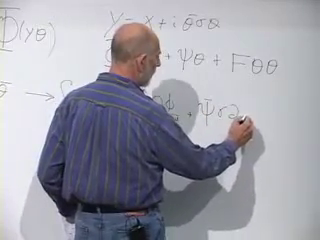
\includegraphics[width=0.76\textwidth]{lecture_09_figure_02.png}
\lectureframe{00:27:36.000}
\caption{Tọa độ chiral và khai triển theo thành phần; ở trên là các hạng vô hướng, fermion và phụ trợ.}
\end{figure}

\section{Tích phân \texorpdfstring{\(d^2\theta\)}{d2-theta} chọn ra điều gì}

Tương tác và khối lượng nảy sinh từ một hàm chỉnh hình \(W(\Phi)\), siêu thế:
\begin{equation}
S_W
=
\int d^4x
\left[
\int d^2\theta\,W(\Phi)
+\mathrm{h.c.}
\right].
\label{eq:l9-superpotential-action}
\end{equation}
Một biểu thức chiral không có sự phụ thuộc \(\bar\theta\) độc lập, nên nếu lấy tích phân của nó trên cả bốn tọa độ lẻ thì sẽ cho không. Thay vào đó, tích phân \(d^2\theta\) chọn ra thành phần \(\theta^2\) của nó.

Để thấy cách đếm tổ hợp trước khi xét một hàm tổng quát, lấy \(W(\Phi)=\Phi^n\). Trong
\begin{equation}
(\phi+\sqrt2\,\theta\psi+\theta^2F)^n,
\end{equation}
có hai cách để thu được đúng hai \(\theta\). Ta có thể chọn một \(F\theta^2\) duy nhất, hoặc chọn hai thừa số fermion.

\begin{classroomqa}
\audiencequestion{Có bao nhiêu hạng chứa một \(F\theta^2\) được chọn và ngoài ra chỉ có các vô hướng: \(n-1\) hay \(n\)? \lecturetimestamp{00:31:33}}
\lecturerresponse{Có \(n\). Bất kỳ một trong \(n\) thừa số nào cũng có thể cung cấp \(F\theta^2\); \(n-1\) thừa số còn lại cung cấp \(\phi\). Đóng góp là \(nF\phi^{n-1}\).}
\end{classroomqa}

\begin{classroomqa}
\audiencequestion{Có bao nhiêu cách để hai thừa số cung cấp hai fermion? \lecturetimestamp{00:32:26}}
\lecturerresponse{Có \(\binom n2=n(n-1)/2\) lựa chọn không có thứ tự. Phép co Grassmann cố định hạng \(\psi\psi\) tương ứng.}
\end{classroomqa}

Do đó, trong ký pháp lược bỏ hệ số của bài giảng,
\begin{equation}
\int d^2\theta\,\Phi^n+\mathrm{h.c.}
\;\leadsto\;
nF\phi^{n-1}
-\frac{n(n-1)}{2}\phi^{n-2}\psi\psi
+\mathrm{h.c.}
\label{eq:l9-power-extraction}
\end{equation}
Dấu trừ được viết ở đây tuân theo khai triển chuẩn hóa chuẩn và quy ước Grassmann; thay đổi quy ước có thể làm dịch chuyển những dấu bề ngoài.

\begin{classroomqa}
\audiencequestion{Điều gì đã xảy ra với hạng \(\phi^n\), hạng hoàn toàn không chứa \(\theta\) nào? \lecturetimestamp{00:33:10}}
\lecturerresponse{Nó có mặt trong tích, nhưng \(d^2\theta\) loại bỏ nó. Mũi tên có nghĩa là phép tích phân chọn hệ số \(\theta^2\); đó không phải là sự bằng nhau của toàn bộ các biểu thức.}
\end{classroomqa}

\begin{figure}[H]
\centering
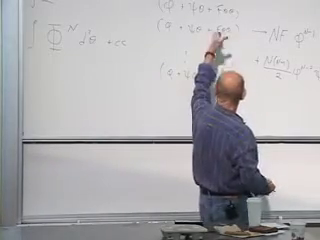
\includegraphics[width=0.82\textwidth]{lecture_09_figure_03.png}
\lectureframe{00:33:38.000}
\caption{Các thừa số siêu trường lặp lại và mũi tên kéo theo trích ra, chứ không phải đồng nhất với, thành phần hai-\(\theta\) của chúng.}
\end{figure}

Cộng các lũy thừa với những hệ số tùy ý biến các hệ số tổ hợp thành các đạo hàm:
\begin{equation}
\int d^2\theta\,W(\Phi)+\mathrm{h.c.}
\;\leadsto\;
F W'(\phi)
-\frac12 W''(\phi)\psi\psi
+\mathrm{h.c.}
\label{eq:l9-W-components}
\end{equation}

\begin{classroomqa}
\audiencequestion{Vì sao hạng fermion lại chứa \(\phi^{n-2}\), thay vì \(\phi^{n-1}\)? \lecturetimestamp{00:36:32}}
\lecturerresponse{Hai thừa số đã cung cấp các fermion, để lại \(n-2\) thừa số vô hướng. Hệ số là một nửa của đạo hàm bậc hai \(W''(\phi)\).}
\end{classroomqa}

Hạng fermion là quan trọng: nó cho một khối lượng khi \(W''\) là hằng và một tương tác Yukawa khi \(W''\) phụ thuộc vào \(\phi\). Tuy nhiên, đối với phân tích chân không, hạng phụ trợ \(FW'\) mang thông tin trực tiếp hơn.

\section{Khử trường phụ trợ}

Gom các hạng chứa \(F\):
\begin{equation}
\mathcal L_F
=
F^\ast F
+F W'(\phi)
+F^\ast \overline{W'(\phi)}.
\label{eq:l9-LF}
\end{equation}
Vì không có \(\partial_\mu F\), phương trình Euler--Lagrange đầy đủ
\begin{equation}
\partial_\mu
\frac{\partial\mathcal L}{\partial(\partial_\mu F)}
-
\frac{\partial\mathcal L}{\partial F}
=0
\end{equation}
ngay lập tức rút gọn thành một phương trình đại số. Xem \(F\) và \(F^\ast\) là các biến độc lập thì ta được
\begin{align}
\frac{\partial\mathcal L_F}{\partial F}
&=F^\ast+W'(\phi)=0,
&
\frac{\partial\mathcal L_F}{\partial F^\ast}
&=F+\overline{W'(\phi)}=0,
\label{eq:l9-F-eom}
\end{align}
và do đó
\begin{equation}
F^\ast=-W'(\phi),
\qquad
F=-\overline{W'(\phi)}.
\label{eq:l9-F-solution}
\end{equation}

\begin{figure}[H]
\centering
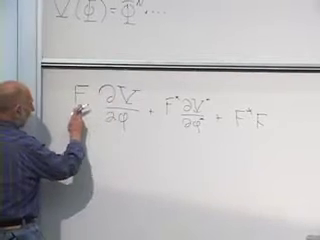
\includegraphics[width=0.82\textwidth]{lecture_09_figure_04.png}
\lectureframe{00:39:40.000}
\caption{Biểu thức đầy đủ của trường phụ và phương trình chuyển động đại số của nó, hiện ra cùng nhau sau khi phần che khuất trên bảng được gỡ bỏ.}
\end{figure}

\begin{classroomqa}
\audiencequestion{Có phải đạo hàm đó nên được lấy theo \(\phi\), thay vì theo trường liên hợp được viết trên bảng không? \lecturetimestamp{00:41:21}}
\lecturerresponse{Đúng. Sửa lại như vậy sẽ khôi phục cặp liên hợp trong phương trình~\eqref{eq:l9-F-eom}: \(F^\ast=-W'(\phi)\) và \(F=-\overline{W'(\phi)}\).}
\end{classroomqa}

Thế vào phương trình~\eqref{eq:l9-LF} ta được
\begin{equation}
\mathcal L_F\big|_{\mathrm{on\ shell}}
=-|W'(\phi)|^2.
\end{equation}
Vì Lagrangian vô hướng có dạng động năng trừ thế năng, nên thế vô hướng thông thường là
\begin{equation}
\boxed{V(\phi,\phi^\ast)=|W'(\phi)|^2\ge0.}
\label{eq:l9-F-potential}
\end{equation}
\(V\) này không phải là siêu thế. Ta dành \(W\) cho hàm chỉnh hình trên siêu không gian và \(V\) cho thế năng thông thường.

\subsection{Hai ví dụ trực tiếp}

Với các chuẩn hóa quy ước chính xác,
\begin{equation}
\begin{gathered}
W(\Phi)=\frac12m\Phi^2,\\
W'(\phi)=m\phi,
\qquad V=|m|^2|\phi|^2.
\end{gathered}
\label{eq:l9-quadratic-W}
\end{equation}
Cùng hạng đó cho khối lượng fermion \(-\tfrac12m\psi\psi+\mathrm{h.c.}\), nên khối lượng của vô hướng và fermion trùng nhau trước khi siêu đối xứng bị phá vỡ.

Đối với
\begin{equation}
W(\Phi)=\frac{g}{3}\Phi^3,
\end{equation}
ta thu được
\begin{equation}
\begin{gathered}
W'(\phi)=g\phi^2,
\qquad V=|g|^2|\phi|^4,\\
\mathcal L_{\mathrm{Yukawa}}
=-g\phi\psi\psi+\mathrm{h.c.}
\end{gathered}
\label{eq:l9-cubic-W}
\end{equation}
Đỉnh vô hướng bậc bốn mô tả tán xạ hai vô hướng, còn hạng Yukawa là đối tác siêu đối xứng của nó.

\section{Hai loại chân không}

Chân không là một cấu hình trường hằng tại một cực tiểu của \(V\); các hạng đạo hàm của nó triệt tiêu. Vì phương trình~\eqref{eq:l9-F-potential} không âm, nên có thể xảy ra hai trường hợp.

\subsection{Một cực tiểu năng lượng bằng không}

Nếu một \(\phi_0\) nào đó thỏa mãn
\begin{equation}
W'(\phi_0)=0,
\end{equation}
thì
\begin{equation}
V(\phi_0)=0,
\qquad
\langle F\rangle=0.
\label{eq:l9-unbroken-F}
\end{equation}
Chân không là siêu đối xứng. Đây là tương tự của từ độ triệt tiêu: không có thành phần phụ nào chọn ra một phương trong siêu không gian.

\subsection{Một cực tiểu bị nâng lên}

Nếu các phương trình
\begin{equation}
W'(\phi)=0
\label{eq:l9-F-flatness}
\end{equation}
không có nghiệm đồng thời tại cực tiểu, thì
\begin{equation}
V_{\min}>0,
\qquad
\langle F\rangle\neq0,
\label{eq:l9-broken-F}
\end{equation}
và siêu đối xứng bị phá vỡ tự phát. Tác dụng vẫn siêu đối xứng; trạng thái năng lượng thấp nhất của nó thì không.

\begin{figure}[H]
\centering
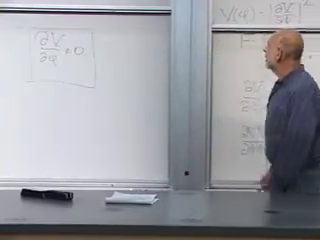
\includegraphics[width=0.88\textwidth]{lecture_09_figure_05.png}
\lectureframe{00:52:09.960}
\caption{Trên bảng vẫn giữ hiện rõ thế dương, phương trình \(F\) và điều kiện chân không, đồng thời phân biệt các phương trình đối xứng với một nghiệm không đối xứng.}
\end{figure}

Phát biểu về tham số trật tự có thể được làm chính xác thông qua phép biến đổi của fermion:
\begin{equation}
\delta\psi_\alpha
=
i\sqrt2
(\sigma^\mu\bar\epsilon)_\alpha\partial_\mu\phi
+\sqrt2\,\epsilon_\alpha F.
\label{eq:l9-fermion-transformation}
\end{equation}
Đối với chân không đồng nhất, hạng đạo hàm triệt tiêu. Nếu
\(\langle F\rangle\neq0\), siêu đối xứng biến đổi fermion bằng cách cộng thêm một hằng khác không, nên chân không không thể bất biến.\editorialnote{Phương trình~\eqref{eq:l9-fermion-transformation} là dạng thành phần chuẩn, làm tường minh phát biểu trong bài giảng rằng các thành phần của siêu trường biến đổi lẫn nhau.}

Cùng kết luận đó cũng suy ra từ siêu đại số. Trong hệ quy chiếu nghỉ,
\begin{equation}
\{Q_\alpha,Q_{\dot\alpha}^\dagger\}
=2\sigma^0_{\alpha\dot\alpha}H.
\end{equation}
Lấy giá trị kỳ vọng chân không biểu diễn năng lượng của nó thành tổng các chuẩn của các siêu điện tích tác dụng lên chân không:
\begin{equation}
E_0\ge0,
\qquad
E_0=0
\ \Longleftrightarrow\
Q_\alpha|0\rangle
=Q_{\dot\alpha}^\dagger|0\rangle=0.
\label{eq:l9-algebra-vacuum-energy}
\end{equation}
Vì vậy, năng lượng chân không dương và sự phá vỡ siêu đối xứng tự phát là hai mặt của cùng một phát biểu về siêu đối xứng cứng.

\begin{center}
\begin{tikzpicture}[x=1.2cm,y=1.0cm,>=Latex]
  \draw[->] (-3,0) -- (-0.2,0) node[right] {\(\phi\)};
  \draw[->] (-2.8,-0.15) -- (-2.8,2.1) node[above] {\(V\)};
  \draw[thick,teal!75!black,domain=-2.5:-0.5,samples=60]
    plot (\x,{0.65*(\x+1.5)^2});
  \fill (-1.5,0) circle (2pt);
  \node[below] at (-1.5,0) {\(F=0\)};
  \draw[->] (0.4,0) -- (3.2,0) node[right] {\(\phi\)};
  \draw[->] (0.6,-0.15) -- (0.6,2.1) node[above] {\(V\)};
  \draw[thick,orange!85!black,domain=0.9:2.9,samples=60]
    plot (\x,{0.55*(\x-1.9)^2+0.65});
  \fill (1.9,0.65) circle (2pt);
  \draw[dashed] (0.6,0.65) -- (1.9,0.65);
  \node[below] at (1.9,0.65) {\(F\neq0\)};
\end{tikzpicture}
\end{center}

\editorialnote{Một minh họa tối thiểu là \(W=f\Phi\), với trường hợp đó \(W'=f\) không bao giờ triệt tiêu và \(V=|f|^2\). Ví dụ một trường ấy có một phương vô hướng phẳng; sự phá vỡ \(F\)-term ổn định, thực tế, thường được thực hiện với nhiều trường chiral, như trong các vùng ẩn kiểu O'Raifeartaigh.}

\section{Sự phá vỡ siêu đối xứng tạo ra gì}

\subsection{Phân tách khối lượng}

Phép tương tự với sắt từ giờ lại quay về phổ năng lượng. Một từ trường nội yếu tách các mức nguyên tử mà không phá hủy bản sắc của nguyên tử. Tương tự, một tham số trật tự phá vỡ siêu đối xứng được truyền yếu sẽ tách các boson và fermion mà nếu không thì sẽ cùng nằm trong một siêu đa bội.

\begin{classroomqa}
\audiencequestion{Những hạt nào được siêu đối xứng biến đổi lẫn nhau và vì thế mất sự suy biến khối lượng khi chân không phá vỡ nó? \lecturetimestamp{00:51:40}}
\lecturerresponse{Boson và fermion. Khối lượng của chúng không nhất thiết còn bằng nhau một khi trạng thái không còn tôn trọng phép biến đổi liên hệ chúng.}
\end{classroomqa}

Sự phân tách không do \(\langle F\rangle\) tự nó tạo ra; nó phụ thuộc vào các tương tác truyền sự phá vỡ tới các trường khả kiến. Nếu các tương tác đó yếu, các hạt khả kiến vẫn còn nhận ra được và các độ phân tách nhỏ so với các thang thống nhất lớn hoặc Planck. Nếu chúng mạnh, phép tương tự sẽ là một nguyên tử bị bóp méo bởi một từ trường khổng lồ đến mức trở thành một vật dài, không còn nhận ra được.

\subsection{Goldstino}

Đối với một bộ sinh bị phá vỡ thông thường, \(J|0\rangle\) cho một trạng thái Goldstone boson. Một siêu điện tích có tính fermion và biến các trạng thái boson thành các trạng thái fermion. Vì chân không được tính là boson, một siêu điện tích bị phá vỡ tạo ra một trạng thái fermion năng lượng bằng không:
\begin{equation}
Q_\alpha|0\rangle
\sim
|\widetilde G_\alpha,\mathbf k=0\rangle.
\label{eq:l9-goldstino}
\end{equation}
Trạng thái lan truyền tương ứng của nó là một fermion Weyl không khối lượng, Goldstone fermion hay goldstino.

\begin{classroomqa}
\audiencequestion{Nếu một phép biến đổi siêu đối xứng không giữ chân không cố định, nó tạo ra trạng thái mới nào? \lecturetimestamp{00:53:24}}
\lecturerresponse{Một fermion không khối lượng. Mô thức thông thường của định lý Goldstone vẫn giữ nguyên, nhưng một bộ sinh fermion biến chân không boson thành goldstino.}
\end{classroomqa}

Do đó, sự phá vỡ siêu đối xứng tự phát cứng có hai dấu hiệu không thể tránh khỏi:
\begin{equation}
\boxed{
V_{\min}>0
\qquad\text{and}\qquad
\text{a massless goldstino}.
}
\label{eq:l9-rigid-breaking-signatures}
\end{equation}

\section{Khu vực ẩn}

Thật tiện khi gọi nguyên tử và vật sắt từ là hai khu vực. Vật sắt từ hình thành tham số trật tự; nguyên tử chỉ cảm nhận trường được truyền từ đó. Khi tương tác ghép yếu, thao tác lên nguyên tử hầu như không kích thích một magnon và hầu như không cho khả năng tiếp cận trực tiếp với môi trường từ. Khi ấy vật sắt từ là ẩn, dù sự hiện diện của nó được suy ra từ những phân tách nhỏ trong phổ.

Xây dựng mô hình siêu đối xứng dùng cùng ngôn ngữ ấy. Các trường bổ sung trong một khu vực ẩn có các giá trị kỳ vọng của hạng \(F\) hoặc \(D\) khác không. Các tương tác gọi là cơ chế truyền đạt chuyển sự phá vỡ ấy sang khu vực khả kiến và sinh ra các khối lượng mềm cho các siêu đối tác. Sự truyền yếu giải thích vì sao lý thuyết khả kiến có thể vẫn gần đúng siêu đối xứng ở một thang cơ bản cao hơn nhiều, đồng thời không biểu lộ sự suy biến boson--fermion chính xác ở năng lượng thấp.

Cấu trúc này không tự động. Cần có các trường bổ sung, một chân không phá vỡ ổn định và một cơ chế truyền đạt được kiểm soát. Đó là vì sao bài giảng mô tả sự phá vỡ siêu đối xứng thực tế là phức tạp và phần nào gượng ép, chứ không phải là một hệ quả duy nhất tất yếu của mô hình tối thiểu.

\section{Hấp dẫn làm thay đổi cả hai dấu hiệu}

\subsection{Năng lượng chân không trở thành một nguồn}

Không có hấp dẫn, việc tịnh tiến mọi năng lượng thêm một hằng số không làm thay đổi các thí nghiệm phi hấp dẫn. Có hấp dẫn, mật độ năng lượng chân không đi vào phương trình Einstein như một hằng số vũ trụ. Một \(V_{\min}\) dương gây ra sự giãn nở gia tốc. Nếu thang của nó so sánh được với thang vật lý hạt cần cho khối lượng các siêu đối tác, độ cong thu được sẽ lớn hơn quan sát một cách khổng lồ.

\begin{classroomqa}
\audiencequestion{Một năng lượng chân không dương khác không tác động lên thế giới như thế nào một khi tính đến hấp dẫn? \lecturetimestamp{01:00:40}}
\lecturerresponse{Nó đóng vai trò như một hằng số vũ trụ và gây ra sự giãn nở gia tốc. Ở các thang vật lý hạt thông thường, hiệu ứng đó sẽ lớn đến mức không thể chấp nhận được.}
\end{classroomqa}

Siêu đối xứng địa phương, hay siêu hấp dẫn, làm thay đổi công thức bình phương dương. Để định hướng, thế \(F\)-term chuẩn \(N=1\) là
\begin{equation}
\begin{aligned}
V_F={}&e^{K/M_P^2}
\left(
K^{i\bar j}D_iW\,D_{\bar j}\overline W
-\frac{3|W|^2}{M_P^2}
\right),\\
D_iW={}&\partial_iW+\frac{\partial_iK}{M_P^2}W.
\end{aligned}
\label{eq:l9-sugra-potential}
\end{equation}
Do có hạng âm, năng lượng dương từ sự phá vỡ siêu đối xứng, về nguyên tắc, có thể bị khử một phần. Phần còn lại có thể là một hằng số vũ trụ nhỏ.

\editorialnote{Bài giảng chủ ý chỉ nêu một hiệu chỉnh có tính sơ đồ và nêu rõ sự phân vân về chỗ đặt khối lượng Planck. Phương trình~\eqref{eq:l9-sugra-potential} ghi lại công thức quy ước cho các đa bội chiral với thế Kähler \(K\); các \(D\)-term gauge sẽ thêm một đóng góp không âm nữa. Nó không giải thích giá trị nhỏ xíu được quan sát, điều vẫn là bài toán hằng số vũ trụ.}

\subsection{Cơ chế siêu-Higgs}

Hiệu ứng hấp dẫn thứ hai dễ hiểu nhất nếu đếm các phân cực. Một hạt có khối lượng spin-\(j\) có \(2j+1\) trạng thái spin trong hệ quy chiếu nghỉ của nó.

\begin{classroomqa}
\audiencequestion{Một hạt có khối lượng spin-\(j\) có bao nhiêu trạng thái spin? \lecturetimestamp{01:05:16}}
\lecturerresponse{\(2j+1\). Cụ thể, một hạt spin một có khối lượng có ba trạng thái, trong khi một boson gauge không khối lượng chỉ có các helicity \(+1\) và \(-1\).}
\end{classroomqa}

Sự khác biệt này là thuần động học. Một hạt có khối lượng có thể được boost về nghỉ, rồi được boost theo một hướng mới trong khi định hướng spin của nó vẫn được giữ, nên mọi hình chiếu đều phải tồn tại. Một hạt không khối lượng không thể bị vượt qua hoặc đưa về nghỉ. Do đó nó chỉ có thể mang hai helicity cực trị.

Đối với trường gauge điện yếu,
\begin{equation}
\underbrace{(+1,-1)}_{\text{massless vector}}
+
\underbrace{(0)}_{\text{Goldstone}}
\longrightarrow
\underbrace{(+1,0,-1)}_{\text{massive vector}}.
\label{eq:l9-higgs-count}
\end{equation}

\begin{classroomqa}
\audiencequestion{Phân cực dọc của một \(W\) hoặc \(Z\) có khối lượng đến từ đâu? \lecturetimestamp{01:08:50}}
\lecturerresponse{Từ boson Goldstone. Nó bị hấp thụ bởi trường gauge và hoàn tất biểu diễn spin một có khối lượng với ba trạng thái.}
\end{classroomqa}

Hấp dẫn có graviton không khối lượng spin hai. Đối tác siêu đối xứng của nó là gravitino không khối lượng spin-\(\tfrac32\).

\begin{classroomqa}
\audiencequestion{Spin của graviton là gì, và vì thế spin của siêu đối tác của nó là gì? \lecturetimestamp{01:10:24}}
\lecturerresponse{Graviton có spin \(2\); đối tác fermion lệch đi một nửa đơn vị và có spin \(3/2\).}
\end{classroomqa}

Một gravitino không khối lượng có các helicity \(\pm\tfrac32\), còn một gravitino có khối lượng còn phải có cả \(\pm\tfrac12\). Goldstino cung cấp chính xác các trạng thái còn thiếu ấy:
\begin{equation}
\begin{gathered}
\underbrace{\left(+\frac32,-\frac32\right)}_{\text{massless gravitino}}
\oplus
\underbrace{\left(+\frac12,-\frac12\right)}_{\text{goldstino}}\\
\Downarrow\\
\underbrace{\left(+\frac32,+\frac12,-\frac12,-\frac32\right)}_{\text{massive gravitino}}.
\end{gathered}
\label{eq:l9-super-higgs}
\end{equation}
Đây là cơ chế siêu-Higgs. Một khi siêu đối xứng là địa phương, goldstino bị hấp thụ và không còn xuất hiện như một hạt không khối lượng độc lập. Gravitino thu được tương tác hấp dẫn và vì vậy khó tạo ra.

\section{Chuyển chủ đề: vì sao \texorpdfstring{\(SU(5)\)}{SU(5)}?}

Hình thức luận siêu đối xứng giờ nhường chỗ cho thống nhất lớn. Nhóm gauge của Mô hình Chuẩn là
\begin{equation}
G_{\mathrm{SM}}
=SU(3)_c\times SU(2)_L\times U(1)_Y.
\label{eq:l9-sm-group}
\end{equation}
Ba thừa số của nó lần lượt tổ chức màu, isospin yếu và siêu điện tích yếu. Câu hỏi thống nhất là liệu tích này có phải là nhóm con còn lại của một nhóm đơn lớn hơn hay không, để các đa bội hạt và các lực gauge có vẻ tách biệt thực ra là những phần của một cấu trúc duy nhất. Ứng viên tối thiểu được phát triển ở đây là \(SU(5)\).

\subsection{Các phần tử nhóm và các bộ sinh}

Đối với \(U\in SU(N)\),
\begin{equation}
U^\dagger U=\mathbf1,
\qquad
\det U=1.
\label{eq:l9-SUN-def}
\end{equation}
Điều kiện thứ nhất là tính unitarity; điều kiện thứ hai chính là ý nghĩa của tính đặc biệt. Viết một phần tử vô cùng bé dưới dạng
\begin{equation}
U=\mathbf1+i\epsilon G+\mathcal O(\epsilon^2).
\label{eq:l9-infinitesimal-U}
\end{equation}
Tính unitarity đòi hỏi
\begin{equation}
G^\dagger=G,
\end{equation}
và
\begin{equation}
\det e^{i\epsilon G}
=e^{i\epsilon\operatorname{tr}G}=1
\end{equation}
đòi hỏi
\begin{equation}
\operatorname{tr}G=0.
\end{equation}
Vì vậy, các bộ sinh là các ma trận Hermite vết bằng không.

Một ma trận Hermite \(N\times N\) chứa \(N^2\) tham số thực: \(N\) phần tử chéo thực và \(N(N-1)/2\) phần tử ngoài đường chéo phức. Điều kiện vết bằng không loại đi một tham số. Do đó
\begin{equation}
\dim SU(N)=N^2-1,
\qquad
\dim SU(5)=24.
\label{eq:l9-SU5-dimension}
\end{equation}
Để so sánh, \(SU(2)\) có ba bộ sinh Pauli và \(SU(3)\) có tám bộ sinh màu.

\section{Các khối của Mô hình Chuẩn bên trong \texorpdfstring{\(SU(5)\)}{SU(5)}}

Tách không gian năm chiều thành một khối yếu hai chiều và một khối màu ba chiều:
\begin{equation}
\mathbf5=\mathbf2\oplus\mathbf3.
\end{equation}
Các bộ sinh được nhúng có dạng
\begin{align}
T^a_L
&=
\begin{pmatrix}
\tfrac12\tau^a&0\\
0&0_{3\times3}
\end{pmatrix},
&& a=1,2,3,
\label{eq:l9-SU2-block}\\
T^A_c
&=
\begin{pmatrix}
0_{2\times2}&0\\
0&\tfrac12\lambda^A
\end{pmatrix},
&& A=1,\ldots,8.
\label{eq:l9-SU3-block}
\end{align}
Các ma trận Pauli \(\tau^a\) sinh ra \(SU(2)\) yếu; các ma trận Gell-Mann \(\lambda^A\) sinh ra \(SU(3)\) màu. Vì các khối không chồng lấn lên nhau, hai nhóm con giao hoán.

Một bộ sinh chéo bổ sung nữa tỷ lệ với ma trận đơn vị trong mỗi khối và vì thế giao hoán với cả hai. Trong biểu diễn cơ bản, một quy ước siêu điện tích gấp đôi thuận tiện là
\begin{equation}
T_Y^{(\mathbf5)}=
\operatorname{diag}
\left(
1,1,-\frac23,-\frac23,-\frac23
\right).
\label{eq:l9-hypercharge-generator}
\end{equation}
Vết của nó triệt tiêu:
\begin{equation}
1+1-3\left(\frac23\right)=0.
\end{equation}
Biểu diễn vật chất liên hợp có các trị riêng đối dấu,
\begin{equation}
Y_{\overline{\mathbf5}}
=
\operatorname{diag}
\left(
-1,-1,\frac23,\frac23,\frac23
\right),
\label{eq:l9-fivebar-hypercharge}
\end{equation}
đó là các giá trị được viết cho cột vật chất trong bài giảng. Dấu tổng thể và chuẩn hóa là theo quy ước; các mục này dùng quy ước của Mô hình Chuẩn
\begin{equation}
Q=T_3+\frac{Y}{2}.
\label{eq:l9-charge}
\end{equation}
Các phương trình~\eqref{eq:l9-SU2-block}--\eqref{eq:l9-hypercharge-generator} cho thấy
\begin{equation}
SU(3)_c\times SU(2)_L\times U(1)_Y
\subset SU(5).
\end{equation}

Ba bộ sinh yếu, tám bộ sinh màu và một bộ sinh siêu tích chiếm \(12\) trong số \(24\) bộ sinh \(SU(5)\).\editorialnote{Mười hai bộ sinh còn lại nằm trong các khối ngoài đường chéo \(2\times3\) và \(3\times2\). Các boson gauge của chúng biến các thành phần kiểu quark và kiểu lepton thành lẫn nhau; đây là nguồn gốc về mặt cấu trúc của các tương tác làm biến đổi baryon và lepton sẽ được triển khai ở phần tiếp theo.}

\begin{classroomqa}
\audiencequestion{Những hạt chuẩn nào tương ứng với các bộ sinh của các phân nhóm quen thuộc? \lecturetimestamp{01:31:05}}
\lecturerresponse{Tám bộ sinh \(SU(3)\) cho tám gluon. Ba bộ sinh \(SU(2)\) cho các trường gauge yếu, sau khi trộn điện-yếu thì trở thành \(W^\pm\) và một phần của hệ \(Z\)-phôtôn; trường \(U(1)\) cung cấp tổ hợp trung hòa còn lại.}
\end{classroomqa}

\section{Một họ trong ngôn ngữ tay trái}

Tập trung vào thế hệ thứ nhất; cùng một khuôn mẫu lặp lại cho các thế hệ muon/charm/strange và tau/top/bottom. Cách tiết kiệm nhất là đếm mọi trường Weyl độc lập như đều là tay trái. Các hạt tay phải được biểu diễn bằng các trường liên hợp điện tích tay trái của chúng:
\begin{equation}
Q_L=(u_L,d_L),\quad
L_L=(\nu_{eL},e_L),\quad
u^c_L,\quad d^c_L,\quad e^c_L.
\end{equation}
Số lượng tương ứng là
\begin{equation}
\underbrace{6}_{Q_L}
+
\underbrace{2}_{L_L}
+
\underbrace{3}_{u^c_L}
+
\underbrace{3}_{d^c_L}
+
\underbrace{1}_{e^c_L}
=15.
\label{eq:l9-fifteen-fields}
\end{equation}

\editorialnote{Mô hình Chuẩn tối thiểu không chứa trường Weyl neutrino tay phải độc lập nào, nên số đếm là \(15\). Riêng phép đếm này không khẳng định neutrino là một hạt Majorana. Thêm một singlet \(\nu^c_L\) đưa tổng số lên \(16\) trường và tự nhiên dẫn tới \(SO(10)\), vượt ra ngoài phép xây dựng \(SU(5)\) hiện tại.}

Đa bội năm chiều phải đặt các thành phần bộ đôi yếu không màu vào hai vị trí đầu và các singlet yếu mang màu vào ba vị trí cuối.

\begin{classroomqa}
\audiencequestion{Cột được đề xuất có sáu trường chứ không phải năm sao? \lecturetimestamp{01:36:14}}
\lecturerresponse{Không. Quark up đã được viết ra trong lượt đầu tiên bị xóa đi. Cột đó là neutrino, electron và ba bản sao màu của phản quark down: tổng cộng là năm thành phần.}
\end{classroomqa}

Khi đó ta được
\begin{equation}
\overline{\mathbf5}
=
\begin{pmatrix}
\nu_{eL}\\
e_L\\
d^c_{rL}\\
d^c_{gL}\\
d^c_{bL}
\end{pmatrix}.
\label{eq:l9-fivebar}
\end{equation}
\editorialnote{Ban đầu bài giảng chỉ gọi đây đơn giản là một đa bội năm chiều. Trong ký hiệu \(SU(5)\) chuẩn, với mọi trường đều viết tay trái, các gán màu và siêu tích của nó xác định nó là biểu diễn liên hợp \(\overline{\mathbf5}\).}
Hai thành phần đầu biến đổi dưới \(SU(2)_L\) nhưng không mang màu. Ba thành phần cuối biến đổi như một phản-bộ ba dưới đối xứng màu nhưng là các singlet yếu.

\begin{classroomqa}
\audiencequestion{Những quark nào mang màu nhưng không mang số lượng tử \(SU(2)_L\), khi mọi trường đều được viết tay trái? \lecturetimestamp{01:40:13}}
\lecturerresponse{Các liên hợp điện tích của các quark tay phải. Với đa bội năm thành phần này, phép kiểm tra điện tích chọn ra ba trường phản quark down \(d^c_{r,g,b}\).}
\end{classroomqa}

Các điện tích trong phương trình~\eqref{eq:l9-fivebar} có tổng bằng 0:
\begin{equation}
0-1+\frac13+\frac13+\frac13=0.
\label{eq:l9-fivebar-charge-sum}
\end{equation}
Điều đó là bắt buộc vì toán tử điện tích là một tổ hợp không vết của các bộ sinh \(SU(5)\).

\begin{classroomqa}
\audiencequestion{Tại sao các phản quark down, chứ không phải các phản quark up, chiếm ba vị trí màu? \lecturetimestamp{01:43:38}}
\lecturerresponse{Neutrino và electron đóng góp tổng điện tích \(-1\). Ba màu của phản quark down đóng góp \(+1\), làm cho vết bằng 0. Ba trường phản-up sẽ cho tổng điện tích sai.}
\end{classroomqa}

Mười trường tay trái còn lại là
\begin{equation}
Q_L\;(6)
\oplus
u^c_L\;(3)
\oplus
e^c_L\;(1),
\end{equation}
và chúng khớp chính xác với biểu diễn phản đối xứng hạng hai
\begin{equation}
\mathbf{10}\cong\wedge^2\mathbf5,
\qquad
\dim\wedge^2\mathbf5=\binom52=10.
\label{eq:l9-ten-preview}
\end{equation}
Việc sắp xếp tường minh của chúng là nhiệm vụ của bài giảng tiếp theo. Sự khớp về số lượng
\begin{equation}
\overline{\mathbf5}\oplus\mathbf{10}
\end{equation}
cho mỗi họ của Mô hình Chuẩn là bằng chứng nổi bật đầu tiên cho thấy ý tưởng \(SU(5)\) không chỉ là một cách gán nhãn lại tùy ý.

\begin{classroomqa}
\audiencequestion{Nếu bộ năm và bộ mười là các biểu diễn khác nhau, điều đó có nghĩa là các hạt của chúng không thể tương tác với nhau sao? \lecturetimestamp{01:46:14}}
\lecturerresponse{Không. Một phép biến đổi nhóm tác dụng bên trong từng biểu diễn bất khả quy, nên nó không trực tiếp biến một phần tử của bộ năm thành một phần tử của bộ mười. Tuy vậy, hai tập đó vẫn có thể tương tác bằng cách phát và hấp thụ các boson gauge chung, và các ghép nối Higgs cũng có thể nối các trường của chúng.}
\end{classroomqa}

\section{Toàn cảnh}

Bài giảng đã lần theo một khuôn mẫu xuyên suốt những thang đo rất khác nhau. Bất biến quay làm cho các mức nguyên tử suy biến; một nền từ trường tách chúng ra. Một chất sắt từ tạo ra nền như vậy trong khi các định luật cơ sở vẫn đối xứng, và các magnon không khe năng lượng của nó cho thấy sự bất đối xứng nằm ở chân không. Trong một lý thuyết siêu đối xứng chiral, giá trị kỳ vọng của trường phụ trợ đóng vai trò tham số trật tự:
\begin{equation}
\begin{aligned}
\langle F\rangle=0
&\quad\Longleftrightarrow\quad
\text{unbroken supersymmetry},\\
\langle F\rangle\neq0
&\quad\Longrightarrow\quad
\text{spontaneous breaking}.
\end{aligned}
\end{equation}
Chân không bị phá vỡ mang năng lượng dương trong siêu đối xứng cứng, tách các siêu đa bội và tạo ra một goldstino. Sự trung gian yếu gợi ý một sector ẩn; hấp dẫn biến năng lượng chân không thành một vấn đề vũ trụ học và hấp thụ goldstino vào một gravitino có khối lượng.

Phép xây dựng \(SU(5)\) ở phần kết mở ra một câu hỏi mới chứ không hoàn tất nó. Các bộ sinh \(5\times5\) Hermite không vết chứa các khối của Mô hình Chuẩn, và năm trường vật chất đầu tiên khớp chính xác dưới dạng \((\nu_e,e^-,d^c_r,d^c_g,d^c_b)\). Mười trường còn lại đang chờ trong biểu diễn phản đối xứng. Chính sự khớp còn dang dở đó là nơi sự thống nhất lớn thật sự bắt đầu.

\chapter{Các đa bội \texorpdfstring{\(SU(5)\)}{SU(5)}, các boson chuẩn leptoquark và sự phân rã proton}

\lectureoverview{Thống nhất lớn trở nên cụ thể khi nhóm của Mô hình Chuẩn được nhúng vào \(SU(5)\). Để thấy phát biểu ấy có nghĩa gì, trước hết ta xây dựng lý thuyết biểu diễn cần thiết: biểu diễn cơ bản \(N\), biểu diễn liên hợp của nó \(\overline N\), các tích tensor, các tensor đối xứng và phản đối xứng, và biểu diễn adjoint. Khi đó, một thế hệ của Mô hình Chuẩn được xếp vào tổ hợp gọn đến bất ngờ \(\overline{\mathbf 5}\oplus\mathbf{10}\). Chính đối xứng làm cho cách sắp xếp này đẹp cũng đồng thời đòi hỏi các boson chuẩn mang màu biến quark thành lepton. Sự trao đổi của chúng cho phép proton phân rã, buộc thang thống nhất tiến tới \(10^{15}\)--\(10^{16}\,\mathrm{GeV}\). Các hằng số liên kết chuẩn chạy cũng chỉ về một thang tương tự, và siêu đối xứng trở lại ở phần cuối vì nó làm cho sự gặp nhau về giá trị số của chúng sắc nét hơn đáng kể.}

\section{Vì sao bắt đầu bằng các biểu diễn nhóm?}

Có nhiều lý thuyết thống nhất lớn đã được đề xuất. Thay vì khảo sát tất cả, ta sẽ mổ xẻ một ví dụ và đặt ra ba câu hỏi: điều gì làm cho nó hoạt động, nó đòi hỏi những hạt mới nào, và thực nghiệm đẩy nó vào chỗ nguy hiểm ở đâu. Nhóm ở đây là \(SU(5)\), và đặc trưng cấu trúc quyết định của nó là phép nhúng
\begin{equation}
SU(3)_c\times SU(2)_L\times U(1)_Y
\subset SU(5).
\label{eq:l10-sm-embedding}
\end{equation}
Ở đây \(SU(3)_c\) tác dụng lên màu, \(SU(2)_L\) tác dụng lên isospin yếu, và \(U(1)_Y\) tác dụng lên siêu tích.

Siêu đối xứng không phải là tiền đề của cấu trúc này. Cả siêu đối xứng lẫn thống nhất lớn đều không kéo theo nhau về mặt lôgic. Mối liên hệ của chúng trong bài giảng này là về số trị: khi phổ các siêu đối tác được đưa vào phép tính nhóm tái chuẩn hóa, ba hằng số liên kết chuẩn tiến tới một giá trị chung chính xác hơn.

Những hạt mà một đối xứng trộn lẫn với nhau tạo thành một biểu diễn của nhóm đối xứng đó. Vì vậy, để phân loại các đa bội hạt trong lý thuyết thống nhất, trước hết cần một chút lý thuyết biểu diễn.

\subsection{Ví dụ \texorpdfstring{\(SU(2)\)}{SU(2)} quen thuộc}

\(SU(2)\) gắn với mômen động lượng góc thông thường có liên hệ chặt chẽ với các phép quay của không gian ba chiều. Chính xác hơn, \(SU(2)\) là phủ đôi của \(SO(3)\). Các biểu diễn bất khả quy của nó được gắn nhãn bởi
\begin{equation}
j=0,\frac12,1,\frac32,\ldots,
\qquad
\dim(j)=2j+1.
\label{eq:l10-su2-spins}
\end{equation}
Vì thế một vô hướng là một singlet, một hạt spin-\(\tfrac12\) là một doublet, và một hạt spin một là một triplet. Nhóm yếu \(SU(2)_L\) là một đối xứng vật lý khác, mặc dù lý thuyết nhóm trừu tượng của nó là như nhau.

\section{Biểu diễn cơ bản và biểu diễn liên hợp của nó}

Đối với \(SU(N)\), biểu diễn cơ bản là không gian các cột phức gồm \(N\) thành phần,
\begin{equation}
\psi=
\begin{pmatrix}
\psi_1\\
\psi_2\\
\vdots\\
\psi_N
\end{pmatrix},
\qquad
\psi'_i=U_i{}^j\psi_j,
\qquad
U\in SU(N).
\label{eq:l10-defining}
\end{equation}
Nó được gọi là biểu diễn cơ bản, hay đơn giản là \(\mathbf N\). Các ma trận \(U\) có kích thước \(N\times N\), và không gian vectơ mà chúng tác dụng lên có số chiều \(N\).

Phép liên hợp phức cho một biểu diễn \(N\)-chiều khác,
\begin{equation}
\psi_i^*\longmapsto U_i{}^{j*}\psi_j^*,
\label{eq:l10-conjugate}
\end{equation}
được ký hiệu là \(\overline{\mathbf N}\). Với \(N>2\), biểu diễn cơ bản và biểu diễn liên hợp là bất tương đương. Ta có thể hoán đổi biểu diễn nào được gọi là biểu diễn của hạt và biểu diễn nào được gọi là biểu diễn của phản hạt, nhưng một khi đã chọn quy ước thì phải giữ cố định.

\begin{classroomqa}
\audiencequestion{\(N\) trong \(SU(N)\) có phụ thuộc vào việc \(N\) là chẵn hay lẻ không, và nó có chỉ các ma trận không? \lecturetimestamp{00:07:33}}
\lecturerresponse{Ở đây không có sự hạn chế chẵn--lẻ nào. \(N\) là kích thước của các ma trận cơ bản, đồng thời cũng là số chiều của biểu diễn cơ bản của chúng. Cả \(\mathbf N\) lẫn \(\overline{\mathbf N}\) đều có số chiều đó.}
\end{classroomqa}

Phản hạt của một phản hạt chính là hạt ban đầu. Đó là vì sao việc hoán đổi tên gọi \(\mathbf N\) và \(\overline{\mathbf N}\) chỉ thay đổi quy ước chứ không thay đổi vật lý.

\section{Tích tensor và tính bất khả quy}

Giả sử một đối tượng có thể chiếm \(N\) trạng thái nội, và một đối tượng khác cũng có thể độc lập chiếm cùng số trạng thái ấy. Bỏ qua vị trí, động lượng, spin và mọi số lượng tử khác ngoài nhãn \(SU(N)\) này, cặp đó có
\begin{equation}
N\times N=N^2
\label{eq:l10-product-count}
\end{equation}
trạng thái. Nếu đối tượng thứ nhất ở trạng thái \(\psi_i\) và đối tượng thứ hai ở trạng thái \(\phi_j\), tích của chúng có thể viết là
\begin{equation}
\Psi_{ij}=\psi_i\phi_j,
\qquad
\Psi'_{ij}=U_i{}^kU_j{}^\ell\Psi_{k\ell}.
\label{eq:l10-tensor-transform}
\end{equation}
Đó là tích tensor \(\mathbf N\otimes\mathbf N\).

\begin{classroomqa}
\audiencequestion{Vì sao đáp án là \(N^2\) chứ không phải \(N^2-1\), và việc cho phép cả hai hạt mang cùng một nhãn nội có vi phạm nguyên lý loại trừ không? \lecturetimestamp{00:10:22}}
\lecturerresponse{Ở đây hai vị trí là khả phân biệt: một đối tượng được cố định ở một vị trí còn đối tượng kia ở một vị trí khác. Nguyên lý Pauli ràng buộc trạng thái lượng tử đầy đủ, kể cả vị trí. Nó không loại bỏ bất kỳ tổ hợp nhãn nội \(N^2\) nào trong số này. Con số \(N^2-1\) sẽ xuất hiện về sau từ một điều kiện không vết trong một tích khác.}
\end{classroomqa}

Biểu diễn tích \(N^2\)-chiều nói chung là khả quy. Một biểu diễn là khả quy khi nó chứa một không gian con thực sự mà nhóm ánh xạ vào chính nó. Các không gian con bất biến có thể được tách ra và xem như những biểu diễn nhỏ hơn; nếu không tồn tại không gian con thực sự nào như vậy thì biểu diễn là bất khả quy.

\subsection{Tensor đối xứng và phản đối xứng}

Mọi tensor hai chỉ số đều tách duy nhất thành
\begin{align}
\Psi_{ij}
&=\Psi^{(S)}_{ij}+\Psi^{(A)}_{ij},\\
\Psi^{(S)}_{ij}
&=\frac12(\Psi_{ij}+\Psi_{ji}),\\
\Psi^{(A)}_{ij}
&=\frac12(\Psi_{ij}-\Psi_{ji}).
\label{eq:l10-sym-anti}
\end{align}
Hai phần này thỏa mãn
\begin{equation}
\Psi^{(S)}_{ij}=\Psi^{(S)}_{ji},
\qquad
\Psi^{(A)}_{ij}=-\Psi^{(A)}_{ji}.
\end{equation}
Phương trình~\eqref{eq:l10-tensor-transform} bảo toàn từng điều kiện, nên các phép biến đổi nhóm không bao giờ trộn lẫn phần đối xứng với phần phản đối xứng.

\editorialnote{Bài giảng để phần đếm tổng quát lại như một bài tập. Số chiều của phần đối xứng và phần phản đối xứng lần lượt là \(N(N+1)/2\) và \(N(N-1)/2\), và tổng của chúng là \(N^2\).}

\begin{figure}[htbp]
\centering
\includegraphics[width=0.78\textwidth]{lecture_10_figure_02.png}
\lectureframe{00:17:57.500}
\caption{Phép phân rã hoàn chỉnh trên bảng cho hai trạng thái spin-\(\tfrac12\): ba trạng thái đối xứng và một trạng thái phản đối xứng.}
\label{fig:l10-spin-decomposition}
\end{figure}

Đối với doublet cơ bản của \(SU(2)\),
\begin{equation}
\mathbf2\otimes\mathbf2=\mathbf3_S\oplus\mathbf1_A.
\label{eq:l10-two-two}
\end{equation}
Viết hai trạng thái cơ sở là \(u\) và \(d\), triplet đối xứng là
\begin{align}
\ket{1,1}&=\ket{uu},\\
\ket{1,0}&=\frac{1}{\sqrt2}\bigl(\ket{ud}+\ket{du}\bigr),\\
\ket{1,-1}&=\ket{dd},
\end{align}
trong khi singlet phản đối xứng là
\begin{equation}
\ket{0,0}
=\frac{1}{\sqrt2}\bigl(\ket{ud}-\ket{du}\bigr).
\end{equation}
Đây là phép cộng quen thuộc của hai mômen động lượng góc spin-\(\tfrac12\): bốn trạng thái ban đầu được tổ chức lại thành spin một và spin không.

\section{Một hạt và một phản hạt: biểu diễn adjoint}

Bây giờ hãy kết hợp biểu diễn cơ bản với biểu diễn liên hợp của nó. Tích này vẫn có \(N^2\) thành phần, nhưng nó biến đổi như một ma trận:
\begin{equation}
M_i{}^j\in\mathbf N\otimes\overline{\mathbf N},
\qquad
M\longmapsto U M U^\dagger.
\label{eq:l10-matrix-transform}
\end{equation}
Khác với \(\mathbf N\otimes\mathbf N\), không có đối xứng hoán vị có ý nghĩa nào giữa một chỉ số cơ bản và một chỉ số phản cơ bản. Thay vào đó, phép tách tự nhiên là
\begin{equation}
M
=
\frac{\operatorname{tr}M}{N}\,\mathbf1_N
+
\left(M-\frac{\operatorname{tr}M}{N}\,\mathbf1_N\right).
\label{eq:l10-trace-split}
\end{equation}
Hạng đầu là một singlet còn phần không vết là biểu diễn adjoint:
\begin{equation}
\mathbf N\otimes\overline{\mathbf N}
=\mathbf1\oplus\mathbf{Adj},
\qquad
\dim\mathbf{Adj}=N^2-1.
\label{eq:l10-adjoint}
\end{equation}

\begin{figure}[htbp]
\centering
\includegraphics[width=0.67\textwidth]{lecture_10_figure_04.png}
\lectureframe{00:23:47.500}
\caption{Kết luận trên bảng cho \(\mathbf N\otimes\overline{\mathbf N}\): các thành phần không vết \(N^2-1\) của nó tạo thành biểu diễn adjoint.}
\label{fig:l10-adjoint}
\end{figure}

Với \(SU(3)\), điều này cho octet quen thuộc,
\begin{equation}
\mathbf3\otimes\overline{\mathbf3}
=\mathbf8\oplus\mathbf1,
\end{equation}
và tám gluon biến đổi theo biểu diễn adjoint. Với \(SU(2)\), biểu diễn adjoint có số chiều ba và biến đổi như spin một.

\section{Một thế hệ của Mô hình Chuẩn}

Có ba thế hệ đã được quan sát, nhưng \(SU(5)\) lặp lại cùng một cấu trúc ấy một cách riêng rẽ cho từng thế hệ. Nó không giải thích vì sao lại có ba bản sao. Vì vậy ta tập trung vào thế hệ thứ nhất.

Tất cả các trường sẽ được viết dưới dạng các trường Weyl tay trái. Một fermion tay phải được biểu diễn bởi trường liên hợp điện tích tay trái của nó:
\begin{equation}
u^c_L,\qquad d^c_L,\qquad e^c_L.
\label{eq:l10-left-handed-bookkeeping}
\end{equation}
Chỉ số mũ \(c\) biểu thị phép liên hợp điện tích; chẳng hạn, \(d^c_L\) là một trường phản quark down tay trái có điện tích điện \(+\tfrac13\).

Theo ký hiệu \(SU(5)\) chuẩn, năm trong số mười lăm trường tay trái được gom vào
\begin{equation}
\overline{\mathbf5}
=
\begin{pmatrix}
\nu_{eL}\\
e_L\\
d^c_{rL}\\
d^c_{gL}\\
d^c_{bL}
\end{pmatrix}.
\label{eq:l10-fivebar}
\end{equation}
Thứ tự được chọn là một khối hai chiều yếu trước, tiếp theo là một khối ba chiều màu. Các phép biến đổi yếu trộn hai thành phần đầu, các phép biến đổi màu trộn ba thành phần cuối, còn các phần sinh ngoài đường chéo của \(SU(5)\) nối hai khối đó.

\editorialnote{Bài giảng gọi cột trong phương trình~\eqref{eq:l10-fivebar} là một \(\mathbf5\) và về sau gọi đa bội phản đối xứng là \(\overline{\mathbf{10}}\). Đó là quy ước liên hợp toàn cục. Ở đây chúng tôi dùng chuẩn hiện đại \(\overline{\mathbf5}\oplus\mathbf{10}\); lấy liên hợp mọi biểu diễn sẽ tái tạo các nhãn của bài giảng mà không thay đổi vật lý của nó.}

Toàn bộ danh mục tối thiểu của thế hệ thứ nhất là
\begin{equation}
\begin{gathered}
\underbrace{Q_L=(u_L,d_L)}_{6}
\oplus
\underbrace{L_L=(\nu_{eL},e_L)}_{2},\\
\underbrace{u^c_L}_{3}
\oplus
\underbrace{d^c_L}_{3}
\oplus
\underbrace{e^c_L}_{1},\\
6+2+3+3+1=15.
\end{gathered}
\label{eq:l10-fifteen}
\end{equation}
Mô hình Chuẩn tối thiểu không có \(\nu^c_L\) độc lập, nên nó không cho khối lượng neutrino khả tái chuẩn hóa. Dao động neutrino cho thấy phát biểu tối thiểu này là không đầy đủ: tự nhiên có các khối lượng neutrino nhỏ nhưng khác không, và cần một mở rộng.

\begin{classroomqa}
\audiencequestion{Khi một khối lượng fermion biến một trạng thái tay trái thành một trạng thái tay phải, nó có đồng thời biến hạt đó thành phản hạt của nó không? \lecturetimestamp{00:34:00}}
\lecturerresponse{Không. Khối lượng electron nối một electron tay trái với một electron tay phải có cùng điện tích điện. Trong ký hiệu hoàn toàn tay trái, trường thứ hai được biểu diễn bởi \(e^c_L\), nhưng hạt bốn thành phần vẫn là một electron. Chỉ một trường trung hòa mới có thể có khối lượng Majorana đồng nhất hạt với phản hạt.}
\end{classroomqa}

\section{Các boson chuẩn thấy được trong ngũ bội}

Mỗi phần sinh của một đối xứng chuẩn đều có một trường chuẩn đi kèm. Ngay trong phương trình~\eqref{eq:l10-fivebar}, ta đã có thể nhận ra các chuyển tiếp quen thuộc:
\begin{itemize}
\item các trường chuẩn yếu tác dụng giữa \(\nu_{eL}\) và \(e_L\);
\item các gluon tác dụng giữa ba màu của \(d^c_L\);
\item các phần sinh trung hòa tác dụng theo đường chéo;
\item các phần sinh ngoài đường chéo mới biến một thành phần lepton thành một thành phần mang màu, hoặc ngược lại.
\end{itemize}

Có thể hình dung gluon như mang các số lượng tử màu quark--phản quark. Bài giảng dùng mẹo ghi nhớ quen thuộc bằng đường thế giới: lần ngược một phản quark đi ra qua đỉnh phát xạ thì nó trông như một quark chạy về phía trước. Vì thế trường được phát ra mang các số lượng tử của một cặp quark--phản quark. Trong ngôn ngữ biểu diễn, đây chính là phần không vết của \(\mathbf3\otimes\overline{\mathbf3}\).

Với \(SU(5)\),
\begin{equation}
\dim\mathbf{Adj}_{SU(5)}=5^2-1=24.
\end{equation}
Sự phân rã của các trường chuẩn này dưới nhóm con của Mô hình Chuẩn là
\begin{equation}
\mathbf{24}
=
(\mathbf8,\mathbf1)_0
\oplus(\mathbf1,\mathbf3)_0
\oplus(\mathbf1,\mathbf1)_0
\oplus(\mathbf3,\mathbf2)_{-5/6}
\oplus(\overline{\mathbf3},\mathbf2)_{5/6},
\label{eq:l10-adjoint-sm}
\end{equation}
trong đó cặp có thứ tự biểu thị \(SU(3)_c\times SU(2)_L\) còn chỉ số dưới là siêu tích.

\editorialnote{Phương trình~\eqref{eq:l10-adjoint-sm} làm hiển lộ rõ cấu trúc khối được vẽ trong bài giảng. Ba hạng đầu chứa các trường chuẩn màu và điện yếu quen thuộc. Hai hạng cuối là 12 bậc tự do thực thường được gọi là các boson \(X\) và \(Y\).}

\begin{figure}[htbp]
\centering
\begin{tikzpicture}[x=1.05cm,y=0.82cm]
  \draw[thick] (0,0) rectangle (5,5);
  \draw[thick] (2,0) -- (2,5);
  \draw[thick] (0,3) -- (5,3);
  \fill[blue!9] (0,3) rectangle (2,5);
  \fill[orange!10] (2,0) rectangle (5,3);
  \fill[teal!9] (2,3) rectangle (5,5);
  \fill[teal!9] (0,0) rectangle (2,3);
  \node[align=center] at (1,4) {weak and\\neutral fields};
  \node[align=center] at (3.5,1.5) {gluons and\\neutral field};
  \node[align=center] at (3.5,4) {\(X,Y\)};
  \node[align=center] at (1,1.5) {\(\overline X,\overline Y\)};
  \node[above] at (1,5) {\(2\)};
  \node[above] at (3.5,5) {\(3\)};
\end{tikzpicture}
\caption{Cấu trúc khối \(2\oplus3\) của trường chuẩn \(SU(5)\). Các khối ngoài đường chéo nối các lepton với các trường mang màu.}
\label{fig:l10-gauge-blocks}
\end{figure}

Với \(Q=T_3+Y\), doublet yếu mang màu trong phương trình~\eqref{eq:l10-adjoint-sm} có các điện tích \(-\tfrac13\) và \(-\tfrac43\); liên hợp của nó có \(+\tfrac13\) và \(+\tfrac43\). Bài giảng gọi các hạt này là \(X\) và \(Y\) nhưng nói rõ là không ấn định tên nào ứng với điện tích nào. Điều bất biến là kiểu chuyển tiếp và điện tích.

\begin{classroomqa}
\audiencequestion{Có ba phiên bản của mỗi boson chuẩn mới \(X\) hay \(Y\) không? \lecturetimestamp{00:41:28}}
\lecturerresponse{Có. Một chuyển tiếp nối một thành phần quark mang màu với một thành phần lepton không màu, nên boson trao đổi phải mang phần màu còn thiếu. Các trường \(X/Y\) tạo thành các triplet màu và có thể phát ra hoặc hấp thụ gluon.}
\end{classroomqa}

Các hạt mang màu không được quan sát như những trạng thái tiệm cận cô lập. Các boson chuẩn mới phải phân rã hoặc hadron hóa thành các tổ hợp trung hòa màu, đúng như quark vẫn làm.

\section{Vì sao đa bội chứa các phản quark down}

Các phần sinh của \(SU(N)\) là các ma trận Hermite không vết. Để thấy mối liên hệ với từ đặc biệt, hãy viết một phần tử nhóm vô cùng bé dưới dạng
\begin{equation}
U(\epsilon)=e^{i\epsilon T}.
\end{equation}
Tính unita cho \(T^\dagger=T\), còn
\begin{equation}
1=\det U=e^{i\epsilon\operatorname{tr}T}
\end{equation}
với mọi \(\epsilon\) kéo theo
\begin{equation}
\operatorname{tr}T=0.
\label{eq:l10-traceless-generator}
\end{equation}

Điện tích điện là một tổ hợp tuyến tính của các phần sinh. Trên cột vật chất trong phương trình~\eqref{eq:l10-fivebar}, nó tác dụng như
\begin{equation}
Q_{\overline5}
=
\operatorname{diag}
\left(0,-1,\frac13,\frac13,\frac13\right),
\qquad
\operatorname{tr}Q_{\overline5}=0.
\label{eq:l10-charge-fivebar}
\end{equation}
Do đó
\begin{equation}
0-1+3\left(\frac13\right)=0.
\end{equation}
Nếu thay các trường phản-down bằng các trường down thì thay vào đó sẽ có
\begin{equation}
0-1+3\left(-\frac13\right)=-2,
\end{equation}
mà không thể là vết của một phần sinh \(SU(5)\). Vì vậy, sự gán phản-down có vẻ lạ ấy thực ra bị áp đặt bởi cấu trúc nhóm.

\section{Mười fermion còn lại}

Mười trường còn lại xuất hiện từ một tensor phản đối xứng hai chỉ số. Theo quy ước chuẩn, đây là phần phản đối xứng của
\begin{equation}
\mathbf5\otimes\mathbf5
=\mathbf{15}_S\oplus\mathbf{10}_A.
\label{eq:l10-five-five}
\end{equation}
Bài giảng xây dựng nó bằng cách tạm thời viết các số lượng tử liên hợp
\begin{equation}
\chi=
\begin{pmatrix}
\nu^c\\
e^c\\
d_r\\
d_g\\
d_b
\end{pmatrix}.
\label{eq:l10-aux-five}
\end{equation}
Đây là một thủ pháp ghi sổ để lấy tích tensor các biểu diễn, chứ không phải là khẳng định rằng tồn tại một ngũ bội vật lý thứ hai gồm các hạt hợp thành.

Cho
\begin{equation}
\Psi^{ij}=-\Psi^{ji},
\qquad
i,j=1,\ldots,5.
\label{eq:l10-antisym-ten}
\end{equation}
Mọi phần tử trên đường chéo đều bằng không, và tam giác dưới được xác định bởi tam giác trên. Do đó
\begin{equation}
\dim\mathbf{10}
=\binom52
=\frac{5\cdot4}{2}
=10.
\label{eq:l10-ten-count}
\end{equation}

Điện tích của một phần tử là tổng các điện tích của hàng và cột trong Phương trình~\eqref{eq:l10-aux-five}. Điều này lập tức cho \(e^c\) ở ô yếu--yếu, các quark down và up trong các khối yếu--màu, và các trường phản-quark up trong khối màu--màu.

\begin{classroomqa}
\audiencequestion{Khi ghép các nhãn positron và quark down, phần tử thu được có phải là một boson \(X\) không? \lecturetimestamp{00:53:08}}
\lecturerresponse{Không. Ở giai đoạn này ta đang xây dựng biểu diễn fermion, không phải biểu diễn adjoint của boson chuẩn. Các điện tích cộng thành \(1-\tfrac13=\tfrac23\), nên phần tử ấy có các số lượng tử của một quark up.}
\end{classroomqa}

Một lựa chọn nhất quán cho các dấu màu là
\begin{equation}
\Psi^{ij}=
\begin{pmatrix}
0 & e^c & d_r & d_g & d_b\\
-e^c & 0 & u_r & u_g & u_b\\
-d_r & -u_r & 0 & u_b^c & -u_g^c\\
-d_g & -u_g & -u_b^c & 0 & u_r^c\\
-d_b & -u_b & u_g^c & -u_r^c & 0
\end{pmatrix}.
\label{eq:l10-ten-matrix}
\end{equation}
Thay đổi pha của các trường sẽ làm đổi một số dấu được viết ra, nhưng không làm đổi biểu diễn hay nội dung hạt.

\begin{figure}[htbp]
\centering
\includegraphics[width=0.83\textwidth]{lecture_10_figure_05.png}
\lectureframe{00:59:17.500}
\caption{Ma trận vật chất phản đối xứng \(2\oplus3\) hiển thị trọn vẹn sau khi các phần tử và nhãn màu đã được kiểm tra trên lớp.}
\label{fig:l10-ten-board}
\end{figure}

\begin{classroomqa}
\audiencequestion{Biểu diễn mười chiều có nhất thiết phải được viết dưới dạng ma trận không, hay có thể viết thành một cột? \lecturetimestamp{00:56:24}}
\lecturerresponse{Cả hai đều được. Có thể liệt kê 10 thành phần độc lập trong một cột, nhưng ma trận phản đối xứng \(5\times5\) cho thấy \(SU(5)\) tác dụng lên hai chỉ số của nó như thế nào, nên vì vậy giàu thông tin hơn nhiều.}
\end{classroomqa}

\begin{classroomqa}
\audiencequestion{Trong khối màu--màu, phần tử được ghi là \(u\) có thực ra phải là một trường phản-up không? \lecturetimestamp{00:57:51}}
\lecturerresponse{Đúng. Nhãn trên bảng được sửa thành \(u^c\), một trường phản-quark up tay trái. Hai điện tích cơ sở kiểu down cộng lại thành \(-\tfrac23\), đó là điện tích của một phản-quark up.}
\end{classroomqa}

\begin{classroomqa}
\audiencequestion{Các màu đã bị lược bỏ khỏi một số phần tử ma trận. Chúng vẫn được bảo toàn chứ? \lecturetimestamp{00:58:05}}
\lecturerresponse{Có. Ba vị trí màu là đỏ, lục và lam. Các nhãn chỉ bị lược bớt để giảm sự rối mắt.}
\end{classroomqa}

Một cặp phản đối xứng của hai biểu diễn cơ bản màu biến đổi như một phản-màu:
\begin{equation}
\wedge^2\mathbf3\simeq\overline{\mathbf3},
\qquad
(rg,rb,gb)\sim(\overline b,-\overline g,\overline r).
\label{eq:l10-anticolor}
\end{equation}
Đó là lý do vì sao ba phần tử độc lập trong khối màu--màu tạo thành đúng bộ ba màu của phản-up.

Một thế hệ nay đã được tổ chức thành
\begin{equation}
\overline{\mathbf5}\oplus\mathbf{10}.
\label{eq:l10-family}
\end{equation}
Điều đáng chú ý là \(u_L\) và \(u^c_L\) cùng xuất hiện trong một đa bội bất khả quy, trong khi \(d_L\) và \(d^c_L\), hoặc \(e_L\) và \(e^c_L\), lại nằm trong các đa bội khác nhau.

\begin{classroomqa}
\audiencequestion{Nếu các phép biến đổi chuẩn chỉ tác dụng trong từng biểu diễn, thì làm sao một khối lượng có thể nối các trường nằm trong 5-bar và 10? \lecturetimestamp{01:00:40}}
\lecturerresponse{Các boson chuẩn không quay một biểu diễn vật chất bất khả quy này thành biểu diễn kia. Các trường Higgs và các liên kết Yukawa có thể nối các biểu diễn khác nhau đồng thời tạo thành một tương tác bất biến tổng thể theo \(SU(5)\); sau khi trường Higgs nhận giá trị kỳ vọng, các tương tác ấy sinh ra khối lượng.}
\end{classroomqa}

\section{Các boson chuẩn tác dụng như những phép dịch chuyển}

Sau khi biểu diễn đã được lắp ghép xong, tác dụng của một boson chuẩn có thể được đọc như một phép dịch chuyển giữa các phần tử của nó. Một boson trung hòa có thể giữ nguyên một nhãn, một boson yếu dịch chuyển giữa các ô yếu, một gluon dịch chuyển giữa các ô màu, và một boson \(X/Y\) dịch chuyển giữa các ô yếu và màu. Các boson chuẩn mang điện có phản hạt, nên mỗi phép dịch chuyển đều có một quá trình ngược lại.

Đối với tensor phản đối xứng, một phép biến đổi vô cùng bé tác dụng lên mỗi chỉ số:
\begin{equation}
\delta\Psi^{ij}
=
i\epsilon
\left(
T^i{}_k\Psi^{kj}
+
T^j{}_k\Psi^{ik}
\right).
\label{eq:l10-two-index-action}
\end{equation}
Trong cách nhìn ma trận, hạng thứ nhất dịch theo phương dọc còn hạng thứ hai dịch theo phương ngang. Các nhãn thành phần dùng để dựng tensor chỉ là gợi nhớ; Phương trình~\eqref{eq:l10-two-index-action} mới là phát biểu lý thuyết nhóm chính xác.

Các phép dịch chuyển yếu biến \(d\) thành \(u\), tức quá trình ở mức quark đứng sau phân rã beta của neutron. Các phép dịch chuyển màu làm đổi đỏ, lục và lam mà không đổi hương. Các phép dịch chuyển ngoài đường chéo làm một điều mới:
\begin{equation}
\begin{aligned}
d^c&\longleftrightarrow e,
& d^c&\longleftrightarrow\nu,\\
d&\longleftrightarrow u^c,
& u&\longleftrightarrow e^c,
\end{aligned}
\label{eq:l10-leptoquark-shifts}
\end{equation}
với trường \(X/Y\) thích hợp mang độ chênh điện tích và màu.

\begin{classroomqa}
\audiencequestion{Các phép dịch chuyển giữa vị trí thứ tư và thứ năm biểu diễn điều gì, còn một phép dịch chuyển từ vị trí thứ nhất sang thứ tư thì sao? \lecturetimestamp{01:10:36}}
\lecturerresponse{Phép dịch chuyển thứ tư--thứ năm biến một màu thành màu khác và là một chuyển tiếp gluon. Phép dịch chuyển thứ nhất--thứ tư băng qua giữa khối yếu và khối màu, và là một trong các chuyển tiếp \(X/Y\) mới.}
\end{classroomqa}

\begin{classroomqa}
\audiencequestion{Có thể điền tường minh một phần tử của nửa dưới ma trận phản đối xứng không? \lecturetimestamp{01:11:23}}
\lecturerresponse{Có. Mỗi phần tử tam giác dưới là số âm của phần tử tam giác trên chuyển vị. Điền một phần tử sẽ làm quy tắc hiện rõ; điền hết tất cả chúng không thêm trạng thái mới nào.}
\end{classroomqa}

\section{Hệ quả nguy hiểm: phân rã proton}

Một boson \(X/Y\) có thể liên kết một quark với một lepton tại một đỉnh và hai trường kiểu quark tại một đỉnh khác. Ở các xung lượng nhỏ hơn nhiều so với khối lượng của nó, việc lấy tích phân loại bỏ boson nặng cho một tương tác bậc sáu theo thứ nguyên có dạng sơ đồ
\begin{equation}
\mathcal L_{\mathrm{eff}}
\sim
\frac{g_5^2}{M_X^2}\,(qq)(q\ell)
+\text{h.c.}
\label{eq:l10-effective-proton}
\end{equation}
Nó vi phạm riêng rẽ số baryon và số lepton, đồng thời bảo toàn các tổ hợp do tương tác chuẩn thống nhất quy định.

Trên bảng, ta theo dõi một quark down và một quark up qua quá trình trao đổi boson nặng. Quark down trở thành một positron, quark up trở thành một phản-quark up, và một quark up thứ hai không tham gia trực tiếp:
\begin{equation}
uud
\longrightarrow
e^++u\overline u.
\label{eq:l10-quark-decay}
\end{equation}
Trạng thái đầu là một proton. Cặp \(u\overline u\) có thể hadron hóa thành một pion trung hòa, cho
\begin{equation}
p\longrightarrow e^++\pi^0.
\label{eq:l10-proton-pion}
\end{equation}

\begin{figure}[htbp]
\centering
\includegraphics[width=0.82\textwidth]{lecture_10_figure_06.png}
\lectureframe{01:16:02.500}
\caption{Sơ đồ dựng trên bảng đã hoàn tất của sự trao đổi boson nặng bên trong một proton, với quark up không tham gia trực tiếp và kênh positron hiện rõ.}
\label{fig:l10-proton-board}
\end{figure}

Bài giảng cũng nhắc đến \(p\to e^++\gamma\), trong đó cặp quark--phản-quark hủy nhau theo điện từ. Kênh ấy chịu thêm một sự ức chế điện từ so với hadron hóa trực tiếp.

Khả năng này không phải là một chi tiết tô điểm tùy chọn của mô hình. Một khi một nhóm đơn chứa các bộ sinh nối quark với lepton, các quá trình vi phạm số baryon nói chung sẽ được kỳ vọng. Nếu chúng xảy ra trên các thang thời gian yếu hoặc điện từ thông thường, thì hạt nhân, hiđrô và vật chất vĩ mô sẽ không tồn tại.

\section{Vì sao proton sống lâu đến vậy?}

\begin{classroomqa}
\audiencequestion{Hằng số liên kết tạo ra một boson \(X\) có phải cũng là hằng số liên kết thống nhất được phần còn lại của nhóm dùng đến không? \lecturetimestamp{01:18:34}}
\lecturerresponse{Ở thang thống nhất thì đúng vậy. Một lý thuyết chuẩn \(SU(5)\) đơn có một hằng số liên kết chuẩn duy nhất là \(g_5\). Các hằng số liên kết mạnh, yếu và siêu điện tích ở năng lượng thấp khác nhau vì sau khi đối xứng thống nhất bị phá vỡ, chúng chạy khác nhau.}
\end{classroomqa}

Không thể chọn hằng số liên kết nhỏ một cách phi thực tế mà không từ bỏ cấu trúc thống nhất. Nguồn ức chế khả dĩ là propagator nặng:
\begin{equation}
\mathcal A
\sim
\frac{g_5^2}{M_X^2}.
\label{eq:l10-amplitude}
\end{equation}
Bình phương biên độ cho \(g_5^4/M_X^4\). Phân tích thứ nguyên và phần tử ma trận proton hoàn tất ước lượng suất phân rã:
\begin{equation}
\Gamma_p
\sim
C_{\mathrm{had}}\,
\frac{\alpha_5^2\,m_p^5}{M_X^4},
\qquad
\alpha_5=\frac{g_5^2}{4\pi},
\label{eq:l10-rate}
\end{equation}
trong đó \(C_{\mathrm{had}}\) chứa các hệ số nhóm, các hiệu ứng tái chuẩn hóa và phần tử ma trận hadron phi nhiễu loạn.

\editorialnote{Bài giảng tách riêng sự phụ thuộc thiết yếu vào \(g^4/M_X^4\) và lưu ý rằng các thừa số khối lượng proton đã bị lược bỏ. Phương trình~\eqref{eq:l10-rate} khôi phục thứ nguyên khối lượng cần thiết mà không ngụ ý một phép tính thời gian sống chính xác.}

\begin{classroomqa}
\audiencequestion{Liệu thừa số nhỏ \(g^4\), có lẽ cỡ \(10^{-8}\) trong ước lượng gần đúng trên lớp, đã đủ làm thời gian sống dài lên hay chưa? \lecturetimestamp{01:25:13}}
\lecturerresponse{Chưa. Nó có giúp, nhưng khoảng cách giữa một thời gian vi mô của tương tác mạnh và cận dưới thời gian sống của proton trải qua nhiều bậc độ lớn hơn thế rất nhiều. Lũy thừa bậc bốn của khối lượng nặng mới phải cung cấp sự ức chế quyết định.}
\end{classroomqa}

Nếu mọi khối lượng đều cỡ khối lượng proton, thì đơn vị thời gian tự nhiên sẽ xấp xỉ thời gian ánh sáng đi qua một proton:
\begin{equation}
t_p\sim\frac{1\ \mathrm{fm}}{c}\sim10^{-23}\ \mathrm{s}.
\label{eq:l10-proton-time}
\end{equation}
Chỉ riêng sự tồn tại của các proton nguyên thủy cũng đã cho thấy thời gian sống của chúng vượt quá tuổi của vũ trụ, nhưng các phép tìm kiếm trong phòng thí nghiệm còn đi xa hơn rất nhiều. Bài giảng so sánh ước lượng vi mô với giới hạn thực nghiệm được trích dẫn khi đó
\begin{equation}
\tau_p\gtrsim10^{33}\ \mathrm{yr}.
\label{eq:l10-lifetime-bound}
\end{equation}

Không cần phải theo dõi một proton đơn lẻ lâu đến thế. Nếu thời gian sống là \(10^{15}\) năm, thì một mẫu gồm \(10^{15}\) proton sẽ cho xấp xỉ một sự kiện mỗi năm. Tổng quát hơn, với \(N_p\) proton được quan sát trong thời gian \(T\), số phân rã kỳ vọng là
\begin{equation}
\langle n\rangle\simeq\frac{N_pT}{\tau_p}.
\label{eq:l10-event-count}
\end{equation}
Một detector chứa khoảng \(10^{33}\) proton là một bể lớn chứ không phải một vật thể thiên văn: bản thân số proton ấy có khối lượng cỡ \(10^6\) kilôgam. Theo dõi một mẫu như vậy biến một thời gian sống khổng lồ của từng proton thành một tốc độ sự kiện đo được hoặc một cận dưới mạnh hơn.

Kết hợp Phương trình~\eqref{eq:l10-rate} với ràng buộc về thời gian sống sẽ đẩy khối lượng boson chuẩn leptoquark lên cỡ
\begin{equation}
M_X\sim10^{15}\text{--}10^{16}\ \mathrm{GeV},
\label{eq:l10-mx}
\end{equation}
với \(10^{16}\,\mathrm{GeV}\) được dùng trong bài giảng như thang an toàn dễ nhớ. Điều này thấp hơn thang Planck vài bậc độ lớn và vì vậy không tự động mâu thuẫn với lý thuyết trường lượng tử.

\section{\texorpdfstring{\(SU(5)\)}{SU(5)} bị phá vỡ và thang thống nhất}

Các trường \(X/Y\) cùng nằm trong một đa bội adjoint của \(SU(5)\) với các trường chuẩn của Mô hình Chuẩn. Một đối xứng chuẩn chính xác chưa bị phá vỡ sẽ không cho phép một số thành phần có khối lượng gần \(10^{16}\,\mathrm{GeV}\) trong khi photon và các gluon vẫn không khối lượng. Vì thế đối xứng ấy tất yếu phải bị phá vỡ tự phát.

\begin{classroomqa}
\audiencequestion{Nếu đối xứng \(SU(5)\) không bị phá vỡ, liệu tất cả các boson chuẩn của nó có đều không khối lượng không? \lecturetimestamp{01:29:37}}
\lecturerresponse{Có, trong lý thuyết chuẩn đang được bàn đến. Bất biến chuẩn cấm một khối lượng chung đưa vào tường minh. Một cơ chế Higgs có thể cho khối lượng đối với các boson chuẩn gắn với những bộ sinh bị phá vỡ, đồng thời để các trường chuẩn của phân nhóm không bị phá vỡ vẫn không khối lượng.}
\end{classroomqa}

Cơ chế Higgs điện yếu đã minh họa khuôn mẫu này: nó phân biệt photon với \(W^\pm\) và \(Z\). Thống nhất lớn đòi hỏi một tham số trật tự riêng ở thang cao, tham số này phân biệt khối yếu \(2\) với khối màu \(3\) và làm cho các trường \(X/Y\) ngoài đường chéo trở nên cực nặng.

So với \(10^{16}\,\mathrm{GeV}\), ngay cả khối lượng boson yếu \(100\,\mathrm{GeV}\) cũng không đáng kể. Ở đủ cao trên ngưỡng nặng, có thể bỏ qua mọi khối lượng boson chuẩn và toàn bộ đối xứng \(SU(5)\) trở thành một gần đúng tốt. Đó là ý nghĩa của một thang thống nhất: không phải là thế giới năng lượng thấp hiển nhiên có \(SU(5)\), mà là các quá trình đủ năng lượng trở nên không nhạy với các sự phân tách khối lượng do phá vỡ đối xứng.

\section{Sự chạy của các hằng số liên kết}

Các hằng số liên kết chuẩn phụ thuộc lôgarit vào thang năng lượng. Định nghĩa
\begin{equation}
\alpha_i(\mu)=\frac{g_i^2(\mu)}{4\pi},
\end{equation}
thì sự tiến hóa ở một vòng có dạng
\begin{equation}
\alpha_i^{-1}(\mu)
=
\alpha_i^{-1}(\mu_0)
-\frac{b_i}{2\pi}
\ln\!\left(\frac{\mu}{\mu_0}\right).
\label{eq:l10-running}
\end{equation}
Các hệ số \(b_i\) phụ thuộc vào nhóm chuẩn và vào mọi hạt đủ nhẹ để chạy trong các vòng lượng tử liên quan.

\editorialnote{Để so sánh siêu điện tích với các hằng số liên kết không Abel bên trong \(SU(5)\), phải gán cho \(g_1\) chuẩn hóa thống nhất lớn theo quy ước. Đây là nguồn gốc của các hệ số số học lý thuyết nhóm được nhắc đến trong bài giảng.}

Ở các năng lượng trong phòng thí nghiệm, nghịch đảo của ba hằng số liên kết là khác nhau. Theo thứ tự định tính trong bài giảng, \(1/\alpha_1\) là lớn nhất vì liên kết siêu tích là yếu nhất, \(1/\alpha_2\) đứng kế tiếp, và \(1/\alpha_3\) là nhỏ nhất vì tương tác mạnh là mạnh nhất. Các đường cong ở những năng lượng không thể tiếp cận không được đo trực tiếp. Chúng được tính từ các giá trị năng lượng thấp quan sát được, phổ hạt, và các giản đồ vòng xác định các hàm beta. Với thành phần hạt của Mô hình Chuẩn, khi vẽ theo \(\log\mu\), chúng trở thành gần như các đường thẳng.

\begin{figure}[htbp]
\centering
\includegraphics[width=0.74\textwidth]{lecture_10_figure_07.png}
\lectureframe{01:36:32.500}
\caption{Đồ thị trên bảng biểu diễn các nghịch đảo của các hằng số liên kết chuẩn tiến lại gần nhau gần \(10^{16}\,\mathrm{GeV}\). Vùng được khoanh tròn đánh dấu chỗ chúng gặp nhau không hoàn toàn.}
\label{fig:l10-running-board}
\end{figure}

Dưới ngưỡng thống nhất, đối xứng bị phá vỡ, phổ nhẹ không lấp đầy các đa tuyến \(SU(5)\) đầy đủ và suy biến, và ba hệ số của hàm beta khác nhau. Do đó các hằng số liên kết chạy với tốc độ khác nhau. Ở thang năng lượng cao, người ta hỏi liệu chúng có đạt tới một giá trị chung hay không:
\begin{equation}
\alpha_1(M_{\mathrm{GUT}})
\stackrel{?}{=}
\alpha_2(M_{\mathrm{GUT}})
\stackrel{?}{=}
\alpha_3(M_{\mathrm{GUT}}).
\label{eq:l10-unification-condition}
\end{equation}

Chỉ với phổ Mô hình Chuẩn không siêu đối xứng, các đường tiến lại gần nhau quanh \(10^{15}\)--\(10^{16}\,\mathrm{GeV}\) nhưng vẫn lệch nhau một lượng đáng kể; bài giảng mô tả mức độ phù hợp là xấp xỉ 15 phần trăm. Sự trùng hợp quan trọng là đây cũng là thang năng lượng mà tính ổn định của proton đòi hỏi.

\section{Một câu hỏi cuối cùng về neutron}

\begin{classroomqa}
\audiencequestion{Nếu quark up không tham gia trong giản đồ phân rã proton được thay bằng một quark down, thì điều đó có mô tả sự phân rã neutron không, và boson \(X\) có liên quan không? \lecturetimestamp{01:36:40}}
\lecturerresponse{Nó sẽ xác định một kênh neutron của thống nhất lớn như \(n\to e^++\pi^-\), nhưng đó không phải là sự phân rã quen thuộc của một neutron tự do. Phân rã beta thông thường của neutron là \(n\to p+e^-+\overline\nu_e\) và diễn ra thông qua tương tác yếu. Nếu thứ tự khối lượng proton--neutron bị đảo ngược, thì trạng thái bền đối với phân rã beta cũng sẽ đảo ngược theo, còn kênh thống nhất lớn chậm hơn nhiều kia vẫn có thể tồn tại.}
\end{classroomqa}

Sự phân biệt này tách động học khỏi tương tác mới. Nuclôn nào phân rã beta phụ thuộc vào độ chênh khối lượng proton--neutron; sự vi phạm số baryon do trao đổi \(X/Y\) là một cơ chế riêng biệt, bị ức chế cực kỳ mạnh.

\section{Siêu đối xứng và bức tranh rộng hơn}

Việc thêm phổ các siêu đối tác làm thay đổi các hệ số của hàm beta trong phương trình~\eqref{eq:l10-running}. Theo trình bày của bài giảng, khi đó ba hằng số liên kết được ngoại suy gặp nhau với độ chính xác khoảng 1 phần trăm. Điều này không chứng minh siêu đối xứng hay thống nhất lớn, nhưng đó là lý do thực nghiệm khiến hai ý tưởng này thường được thảo luận cùng nhau.

Các đa tuyến vật chất còn có thể được thống nhất thêm nữa. Theo
\begin{equation}
SO(10)\supset SU(5),
\end{equation}
một biểu diễn spinor phân rã thành
\begin{equation}
\mathbf{16}
\longrightarrow
\mathbf{10}\oplus\overline{\mathbf5}\oplus\mathbf1.
\label{eq:l10-so10}
\end{equation}
Biểu diễn singlet được đồng nhất một cách tự nhiên với một phản neutrino tay trái, hay tương đương là liên hợp điện tích của một neutrino tay phải. Vì vậy, cả 16 trường của một họ mở rộng đều nằm gọn trong một đa tuyến \(SO(10)\) bất khả quy.

Các thí nghiệm phân rã proton tiếp tục kiểm tra ý tưởng này bằng cách nâng cận dưới của thời gian sống lên khi không quan sát thấy sự kiện nào. Các mô hình thống nhất lớn siêu đối xứng không cho một thời gian sống proton phổ quát duy nhất: các trường nặng bổ sung và các toán tử phụ thuộc vào siêu đối tác có thể làm thay đổi kênh trội và tốc độ trên một khoảng rất rộng.

\editorialnote{Trong thống nhất lớn siêu đối xứng, sự trao đổi Higgs bộ ba màu có thể sinh ra các toán tử vi phạm số baryon bậc năm, bên cạnh toán tử boson chuẩn bậc sáu được thảo luận ở đây. Các hệ số của chúng phụ thuộc mạnh vào phổ nặng, cấu trúc hương vị và khối lượng các siêu đối tác, điều này giải thích lời lưu ý trong bài giảng rằng chỉ riêng siêu đối xứng không dẫn đến một thời gian sống duy nhất.}

Bài học lâu dài ở đây là một thế căng thẳng chứ không phải một kết luận dứt khoát. Lý thuyết nhóm đặt quark và lepton vào cùng một khuôn khổ với độ gọn đáng kinh ngạc, các hằng số liên kết chạy gợi ý một thang năng lượng cao chung, và siêu đối xứng làm sắc nét thêm gợi ý định lượng đó. Cùng một cấu trúc ấy cũng dự đoán sự chuyển hóa nguy hiểm của quark thành lepton. Vì vậy, bất kỳ phiên bản thành công nào cũng phải giữ được sự tao nhã ấy đồng thời giữ cho proton ổn định trong một thời gian gần như không thể tưởng tượng nổi. Theo tinh thần kết thúc của bài giảng: cầu mong mọi proton của chúng ta đều vẫn ổn định.

\end{document}
